\documentclass[11pt,a4paper]{article}
\usepackage[utf8]{inputenc}
\usepackage[T1]{fontenc}
\usepackage{geometry}
\geometry{margin=2.5cm}
\usepackage{longtable}
\usepackage{booktabs}
\usepackage{array}
\usepackage{colortbl}
\usepackage{xcolor}
\usepackage{graphicx}
\usepackage{hyperref}
\usepackage{enumitem}
\usepackage{titlesec}
\usepackage{fancyhdr}
\usepackage{tabularx}
\usepackage{multirow}
\usepackage{amsmath}
\usepackage{float}

\definecolor{pendiente}{RGB}{178,34,34}
\newcommand{\PENDIENTE}[1]{\textcolor{pendiente}{\textbf{[PENDIENTE -- #1]}}}

\hypersetup{colorlinks=true, linkcolor=blue, citecolor=blue, urlcolor=blue}

\pagestyle{fancy}
\fancyhf{}
\fancyhead[L]{UTEQ -- Ingeniería de Requerimientos (ISR-401 / 20303)}
\fancyhead[R]{ERS -- CarniCore -- Entrega 3 (2A)}
\fancyfoot[C]{\thepage}

\title{
\vspace{-2cm}
\textbf{Especificación de Requisitos de Software (ERS/SRS)}\\[0.3cm]
\Large Sistema CarniCore\\[0.2cm]
\large Sistema de Trazabilidad, Pesaje Inteligente e Inventario para\\
Distribuidora de Cárnicos Pucayacu -- La Maná, Cotopaxi\\[0.4cm]
\normalsize Entrega 3 (2A): Especificación de Requisitos Completa + Componente Empírico\\
Asignatura: Ingeniería de Requerimientos [20303] -- 4to Nivel\\
Estándar: ISO/IEC/IEEE 29148:2018 -- ISO/IEC 25010:2023\\
Repositorio: \url{https://github.com/EdhuXav/CarniCore_Proyecto_ISR401}
}
\author{Universidad Técnica Estatal de Quevedo (UTEQ)\\Facultad de Ciencias de la Computación -- Carrera de Ingeniería de Software}
\date{Versión del documento 3.0 -- Fecha de entrega: 02/08/2026 (corte formal de la Entrega 3 (2A): miércoles 29/07/2026, 00:00, último commit válido)}

\begin{document}
\begin{titlepage}
    \centering

    \textbf{\large UNIVERSIDAD TÉCNICA ESTATAL DE QUEVEDO}\\[0.5cm]

    
\includegraphics[width=4cm]{figures/logo.png}\\[0.4cm]

    \textbf{INGENIERÍA DE REQUERIMIENTOS}\\[0.5cm]



    \textbf{TEMA:}\\[0.3cm]

  PROYECTO FIN DE CURSO: ENTREGA 2A – ERS COMPLETO CON VALIDACIÓN Y TRAZABILIDAD.\\[0.5cm]

    \textbf{INTEGRANTES:}\\[0.5cm]
    CASTRO BAJAÑA ARIEL OMAR\\[0.3cm]
    CRESPO ESPINOZA KLEBER OBED\\[0.3cm]
    GAMARRA ARAUJO EDHU XAVIER\\[0.3cm]
    PEREZ RUIZ CARLOS ANDRES\\[0.3cm]
    QUINTERO GENDE ERICK JAHR\\[0.3cm]

    \textbf{ASIGNATURA:}\\[0.3cm]

    INGENIERÍA DE REQUERIMIENTOS\\[0.3cm]

    \textbf{CURSO:}\\[0.3cm]

    4TO “A” SOFTWARE\\[0.3cm]

    \textbf{FECHA:}\\[0.3cm]

    2/08/2026\\[0.5cm]

    \textbf{DOCENTE:}\\[0.3cm]

    ING. GUERRERO ULLOA GLEISTON CICERON\\[0.5cm]
    Último commit hasta el Domingo 02/08/2026 con 18:00 horas

    \vfill

\end{titlepage}

\newpage
\section*{Historial de Versiones}
\begin{longtable}{|p{1.5cm}|p{2.2cm}|p{3cm}|p{8cm}|}
\hline
\textbf{Versión} & \textbf{Fecha} & \textbf{Autor(es)} & \textbf{Descripción del cambio} \\
\hline
1.0 & 31/05/2026 & Equipo CarniCore & Entrega 1A: planificación del proyecto de IR, introducción y descripción general preliminar. \\
\hline
1.5 & 15/06/2026 & Equipo CarniCore & Correcciones sobre la 1A: alcance delimitado, exclusión explícita del módulo de facturación electrónica del SRI. \\
\hline
2.0 & 12/07/2026 & Equipo CarniCore & Entrega 1B: interfaces externas con mockups, 15 RF, 6 RNF, restricciones de diseño, modelado UML parcial, MoSCoW y matriz de trazabilidad parcial. \\
\hline
3.0 & \ 02/08/2026 & Equipo CarniCore & Entrega 3 (2A): requisitos completados a 25 RF y 15 RNF con los 8 atributos y EV-XX; requisito de explicabilidad evaluado; requisitos legales mapeados a la Ley Orgánica de Protección de Datos Personales; historias de usuario Connextra/INVEST/Gherkin para todo RF \textit{Debe tener}; modelado UML completo; priorización MoSCoW+Kano+WSJF; matriz de trazabilidad extendida (40 filas); componente empírico y puente hacia la publicación. \\
\hline
\end{longtable}

\newpage
\tableofcontents
\newpage

%======================================================
\section{Introducción}
%======================================================
\subsection{Propósito}
El presente documento constituye la Especificación de Requisitos de Software (ERS) del sistema CarniCore, elaborada siguiendo la estructura y terminología del estándar ISO/IEC/IEEE~29148:2018 para la ingeniería de requisitos \cite{iso29148}. Esta versión (Entrega 3 -- 2A) consolida y amplía la Entrega 2 (1B), completando el conjunto de requisitos funcionales y no funcionales, el modelado UML, la priorización combinada y la trazabilidad extendida, de modo que sirva como base contractual y técnica verificable para las siguientes etapas del ciclo de vida del software y como insumo directo del componente empírico y del manuscrito paralelo orientado a publicación.

Este documento está dirigido a tres audiencias: (1) el equipo de desarrollo, que lo usará como insumo para el diseño arquitectónico, la planificación de sprints y la construcción del Producto Mínimo Viable (MVP); (2) el personal docente y evaluador de la asignatura Ingeniería de Requerimientos [20303], que verificará el cumplimiento de los criterios C1--C10 de la rúbrica de la Entrega 3 (2A); y (3) la propietaria de la distribuidora y su equipo administrativo, en calidad de cliente y validador funcional de los requisitos documentados.

\subsection{Alcance}
El software a desarrollar se denomina CarniCore y digitaliza y da trazabilidad a los procesos operativos críticos de una distribuidora de productos cárnicos (res, cerdo, pollo y embutidos), actualmente gestionados de forma manual en cuadernos y hojas de Excel, según se evidenció en la entrevista semiestructurada aplicada a la propietaria.

\paragraph{El sistema SÍ hará:}
\begin{itemize}[nosep]
\item Registrar el ingreso de lotes y animales (cerdo y res con número de arete) provenientes de proveedores certificados, incluida la guía de origen y movilización.
\item Registrar el pesaje de productos y calcular automáticamente el costo por libra, emitiendo un comprobante de pesaje.
\item Registrar el proceso de despiece y clasificación de cortes.
\item Gestionar el inventario en cámaras frigoríficas, diferenciado por sección, y controlar los días de vida útil según el tipo de producto.
\item Registrar bajas de producto por vencimiento o deterioro, con evidencia fotográfica y aprobación del administrador general.
\item Permitir la consulta de trazabilidad completa de un producto desde el proveedor/granja de origen hasta la venta final, incluyendo consulta pública restringida mediante código QR.
\item Generar reportes gerenciales de ventas, compras, pérdidas e inventario por período.
\item Gestionar usuarios con distintos roles y registrar operaciones en modo de contingencia offline ante cortes de energía o conectividad intermitente, sincronizando posteriormente.
\end{itemize}

\paragraph{El sistema NO hará (exclusiones explícitas):}
\begin{itemize}[nosep]
\item No sustituirá al sistema de facturación electrónica del SRI; únicamente referenciará el número de factura generado externamente.
\item No emitirá guías de movilización ante Agrocalidad; solo almacenará y permitirá consultar dichas guías una vez emitidas por la entidad competente.
\item No incluirá, en esta versión, un módulo de comercio electrónico o venta en línea al consumidor final.
\item No controlará de forma automática sensores IoT de temperatura de las cámaras frigoríficas en esta fase (trabajo futuro).
\item No incorpora, en esta entrega, componentes de Inteligencia Artificial o Aprendizaje Automático que produzcan decisiones autónomas; véase la justificación del requisito de explicabilidad en la Sección~3.4.
\end{itemize}

\subsection{Glosario de términos, acrónimos y abreviaturas}
\begin{longtable}{|p{4cm}|p{11cm}|}
\hline
\textbf{Término} & \textbf{Definición} \\
\hline
ERS/SRS & Especificación de Requisitos de Software / Software Requirements Specification. \\
RF / RNF & Requisito Funcional / Requisito No Funcional. \\
CU & Caso de Uso. \\
HU & Historia de Usuario (formato Connextra). \\
CA & Criterio de Aceptación (formato Gherkin: Dado--Cuando--Entonces). \\
EV-\textit{XX} & Identificador de Evidencia que respalda un requisito. \\
RD & Restricción de Diseño. \\
MU-\textit{XX} & Identificador de mockup. \\
Canal & Cuerpo del animal faenado, sin cabeza ni vísceras, listo para despiece. \\
Faenamiento & Proceso de sacrificio y procesamiento del animal en la planta. \\
Guía de origen & Documento oficial de Agrocalidad que certifica la procedencia y el número de arete de los animales movilizados. \\
Guía de movilización & Documento que autoriza el transporte de animales o canales entre provincias. \\
Merma & Diferencia de peso entre el animal vivo y el producto faenado. \\
Arete & Identificador físico único colocado en el animal para su trazabilidad ante Agrocalidad. \\
Agrocalidad & Agencia de Regulación y Control Fito y Zoosanitario del Ecuador. \\
MoSCoW & Técnica de priorización: \textit{Must have, Should have, Could have, Won't have}. \\
Kano & Modelo de clasificación de características de producto según su relación con la satisfacción del cliente. \\
WSJF & \textit{Weighted Shortest Job First}, técnica de SAFe para priorizar por relación costo-de-retraso sobre duración. \\
ISO/IEC 25010 & Norma de calidad de producto de software (SQuaRE) \cite{iso25010}. \\
MVP & Producto Mínimo Viable. \\
LOPDP & Ley Orgánica de Protección de Datos Personales del Ecuador \cite{lopd2021}. \\
\hline
\end{longtable}

\subsection{Referencias}
La bibliografía completa se gestiona en \texttt{referencias.bib} y se cita a lo largo del documento; incluye, entre otras, las normas base \cite{iso29148,iso25010}, los fundamentos de ingeniería de requisitos \cite{pohl2010,swebok2024}, los principios FAIR \cite{wilkinson2016fair}, la literatura reciente sobre IA generativa aplicada a ingeniería de requisitos \cite{cheng2026genai,arora2024genai,vogelsang2024llm} y sobre explicabilidad como RNF \cite{chazette2020explainability,chazette2021exploring,chazette2022explainable}, la Ley Orgánica de Protección de Datos Personales del Ecuador \cite{lopd2021}, las guías de estudios empíricos y de caso \cite{molleri2020checklist,hennink2017saturation,hagaman2017interviews,guest2006interviews,runeson2009casestudy,mendez2017naming,jedlitschka2008reporting,wohlin2012experimentation,nosek2018preregistration,montgomery2022requirementsquality,cohen1960kappa,fleiss1971kappa,ferrari2016ambiguity,fischbach2023acceptance,kitchenham2007slr}, los principios de citación de software \cite{smith2016softwarecitation,druskat2021cff} y la literatura de dominio sobre trazabilidad cárnica y agroalimentaria \cite{chen2021blockchain,beck2021blockchainmeat,varavallo2022greenblockchain,escalona2022traceability,demi2021blockchaintraceability}. El conjunto satisface el mínimo de 25 fuentes primarias exigido en la Sección 3.1 de la guía, con más de 10 publicadas en los últimos tres años.

\subsection{Visión general del documento}
El resto del documento se organiza así: la Sección~2 presenta la descripción general del producto; la Sección~3 detalla los requisitos específicos completos (interfaces, RF, RNF, explicabilidad, requisitos legales, historias de usuario y restricciones de diseño); la Sección~4 presenta el modelado UML completo; la Sección~5 la priorización combinada y la matriz de trazabilidad extendida; la Sección~6 el estado del MVP; la Sección~7 el componente empírico; y los apéndices documentan el plan de IR, las evidencias de elicitación y la estructura del repositorio.

%======================================================
\section{Descripción General}
%======================================================
\subsection{Perspectiva del producto}
CarniCore es un sistema nuevo; la distribuidora no cuenta actualmente con ningún sistema informático de gestión interna. El sistema es independiente y no reemplaza a ningún software existente, aunque referenciará el número de factura generado por el sistema contable externo (SRI) que utiliza la propietaria.

\begin{figure}[H]
    \centering
    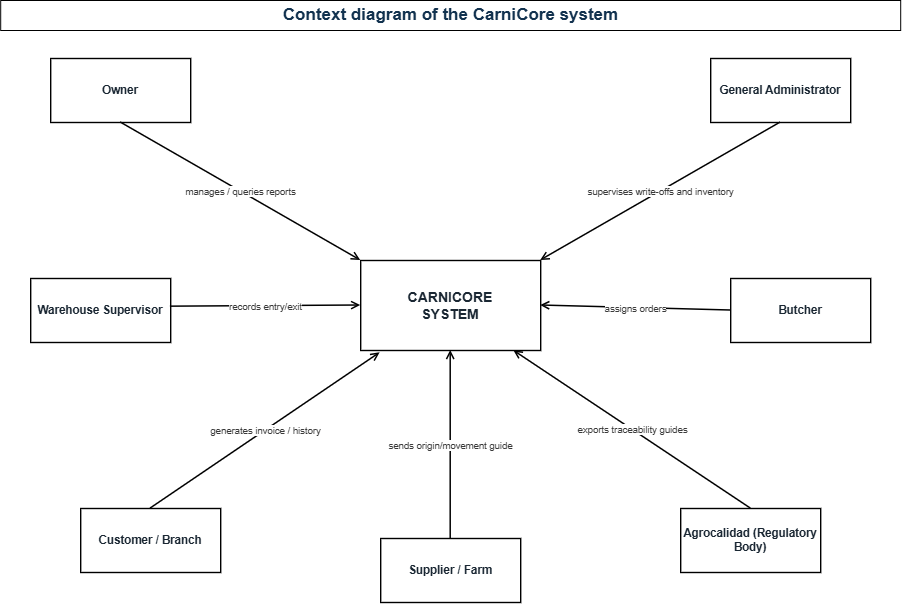
\includegraphics[width=\textwidth,keepaspectratio]{figures/Context_Diagram.png}
    \caption{Diagrama de Contexto del Sistema}
    \label{fig:diagrama_clases}
\end{figure}

\subsection{Funciones del producto}
\begin{enumerate}[nosep]
\item Gestión de proveedores y guías de origen/movilización.
\item Registro de ingreso de lotes y animales.
\item Pesaje inteligente con cálculo automático de costos.
\item Registro de despiece y clasificación de cortes.
\item Gestión de cámaras frigoríficas e inventario por sección.
\item Control de vida útil y alertas de vencimiento.
\item Registro de bajas de producto con evidencia y supervisión.
\item Consulta de trazabilidad extremo a extremo, incluida vía QR.
\item Registro de ventas, salidas y devoluciones de producto.
\item Generación de reportes gerenciales (ventas, compras, pérdidas, inventario).
\item Gestión de usuarios y roles.
\item Operación en modo de contingencia offline con sincronización posterior.
\end{enumerate}

\subsection{Mapa de interesados (stakeholders) y matriz poder/interés}
\begin{longtable}{|p{3.2cm}|p{2.5cm}|p{2cm}|p{2cm}|p{5cm}|}
\hline
\textbf{Interesado} & \textbf{Tipo} & \textbf{Poder} & \textbf{Interés} & \textbf{Estrategia de gestión} \\
\hline
Propietaria (Gisela E. Ibáñez Medina) & Interno / decisor & Alto & Alto & Gestionar de cerca; validación semanal de requisitos. \\
\hline
Administrador general & Administrativo interno & Alto & Alto & Gestionar de cerca; aprueba bajas e inventario. \\
\hline
Encargado de bodega & Operativo interno & Medio & Alto & Mantener informado; usuario intensivo del sistema. \\
\hline
Carnicero & Operativo interno & Bajo & Alto & Mantener informado; usuario del módulo de despiece. \\
\hline
Cliente / Sucursal & Externo & Bajo & Medio & Monitorear; consulta de trazabilidad pública. \\
\hline
Agrocalidad (ente de control) & Externo regulador & Alto & Bajo & Mantener satisfecho; exportación de evidencia de trazabilidad. \\
\hline
Proveedor / Granja & Externo & Bajo & Bajo & Monitorear; provee guías de origen. \\
\hline
Docente supervisor ISR-401 & Interno académico & Alto & Alto & Gestionar de cerca; gatekeeper de evaluación. \\
\hline
\end{longtable}

\subsection{Modelado organizacional i* -- Diagramas SD y SR}

El diagrama de Dependencia Estratégica (i* SD) disponible en el repositorio muestra las siguientes dependencias entre actores:

\begin{itemize}[nosep]
\item \textbf{Propietaria $\leftrightarrow$ CarniCore:} dependencia de dato: reportes gerenciales confiables (meta blanda) desde CarniCore hacia la Propietaria; dependencia de recurso: datos de ventas/compras/pérdidas desde la Propietaria hacia CarniCore.
\item \textbf{Administrador General $\rightarrow$ CarniCore:} dependencia de tarea: aprobar bajas de producto.
\item \textbf{CarniCore $\rightarrow$ Administrador General:} dependencia de meta: alerta de vida útil.
\item \textbf{Encargado de Bodega $\rightarrow$ CarniCore:} dependencia de tarea: registrar ingreso y pesaje.
\item \textbf{Carnicero $\rightarrow$ CarniCore:} dependencia de recurso (peso): registrar cortes.
\end{itemize}

\noindent Archivo correspondiente:
\begin{verbatim}
istar_SD.svg
\end{verbatim}

\begin{figure}[H]
    \centering
    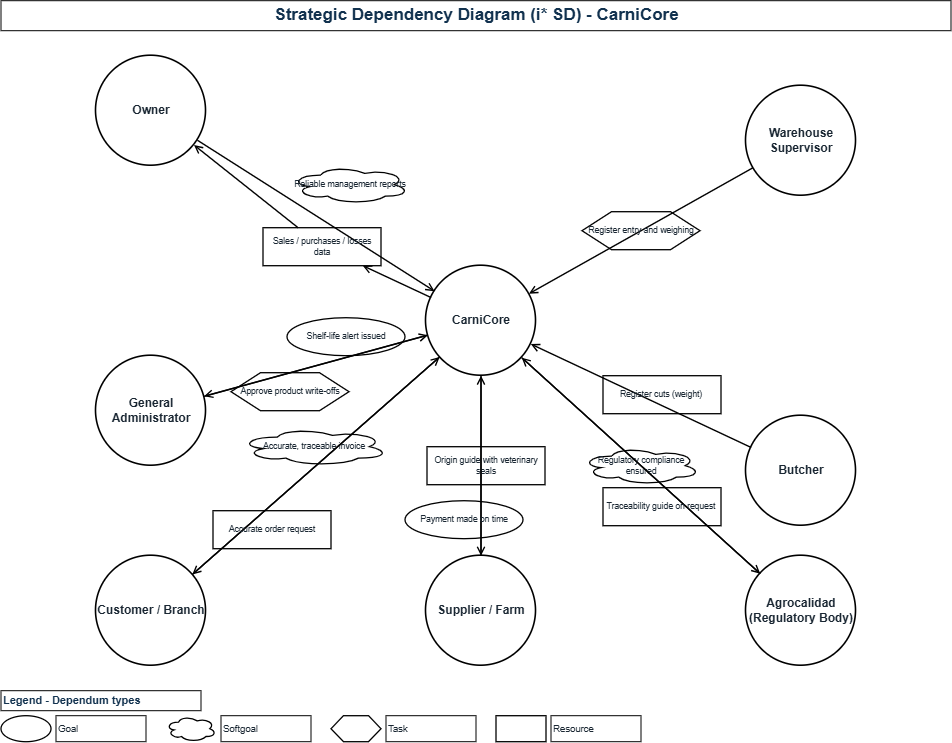
\includegraphics[width=\textwidth,keepaspectratio]{figures/Strategic_Dependency_Diagram.png}
    \caption{Diagrama de Dependencia Estratégica del Sistema}
    \label{fig:diagrama_clases}
\end{figure}


\subsection{Características de los usuarios}
\begin{longtable}{|p{2.8cm}|p{5cm}|p{2cm}|p{2.5cm}|}
\hline
\textbf{Tipo de usuario} & \textbf{Descripción} & \textbf{Nivel técnico} & \textbf{Frecuencia} \\
\hline
Propietaria & Lidera el equipo, coordina compras y ventas; requiere reportes gerenciales resumidos. & Básico & Diaria \\
\hline
Administrador general & Supervisa inventario, autoriza bajas de producto, revisa diferencias. & Medio & Diaria \\
\hline
Encargado de bodega & Registra ingreso, pesaje y distribución de productos a sucursales. & Básico & Diaria (múltiples veces) \\
\hline
Carnicero & Ejecuta el despiece; consulta pedidos asignados. & Básico & Diaria \\
\hline
Cliente / Sucursal & Realiza pedidos y consulta el historial de un producto adquirido. & Básico & Ocasional \\
\hline
\end{longtable}

\subsection{Entorno operativo}
Estaciones de trabajo (PC o tablet) en el punto de pesaje, con posibilidad futura de báscula electrónica con salida serial/USB; dispositivo móvil para el encargado de bodega; navegador web moderno; conectividad intermitente en la planta de La Maná, por lo que se requiere un modo de contingencia offline parcial en bodega (RF-21, RNF-02, RNF-14).

\subsection{Restricciones}
\begin{itemize}[nosep]
\item \textbf{Regulatorias:} compatibilidad con los formatos de guía de origen y movilización de Agrocalidad y con los registros sanitarios firmados por el médico veterinario de planta.
\item \textbf{Tecnológicas:} el módulo de pesaje debe poder integrarse a futuro con básculas electrónicas con salida de impresión de tickets.
\item \textbf{De hardware:} operación en equipos de gama media disponibles en la planta de La Maná, con soporte de operación offline parcial en bodega.
\item \textbf{De interfaz con otros sistemas:} registro manual del número de factura emitido por el sistema contable/SRI externo, sin integración directa en esta fase.
\item \textbf{Organizacionales:} proyecto desarrollado en el marco de la asignatura ISR-401/20303 (UTEQ), con entregas parciales acumulativas 1A, 1B, 2A y 2B según el cronograma de la cátedra.
\item \textbf{Legales:} cumplimiento de la Ley Orgánica de Protección de Datos Personales del Ecuador \cite{lopd2021} para todo dato personal tratado por el sistema (véase Sección~3.5).
\end{itemize}

\subsection{Suposiciones y dependencias}
\begin{itemize}[nosep]
\item Se asume conexión a internet estable en al menos el punto central de bodega para la sincronización de datos.
\item Se asume que el personal de bodega y los carniceros recibirán una capacitación básica de uso del sistema (referencia directa de RNF-04).
\item Se depende de la disponibilidad continua de la propietaria y del administrador general para la validación periódica de requisitos.
\item Se asume que los formatos de guía de origen y movilización de Agrocalidad no cambiarán sustancialmente durante el desarrollo.
\item Se asume que los cortes de energía eléctrica, mencionados por la propietaria como causa de pérdidas, seguirán siendo un riesgo operativo relevante durante la vida del proyecto (referencia directa de RNF-02 y RNF-14).
\end{itemize}

%======================================================
\section{Requisitos Específicos Completos}
%======================================================
\subsection{Requisitos de interfaces externas}
\subsubsection{Interfaces de usuario}
Se definen seis pantallas principales como mockups de baja fidelidad heredadas de la Entrega 1B (P1--P6) más los mockups de alta fidelidad de las pantallas de prioridad \textit{Debe tener}, identificados MU-01 a MU-\textit{XX} y trazados a los RF que soportan (véase Sección~3.6 y la matriz de la Sección~5.2).





\subsubsection{Interfaces de hardware}
Estación de trabajo (PC o tablet) en el punto de pesaje con posibilidad futura de báscula electrónica (salida serial/USB); impresora térmica de tickets (trabajo futuro); dispositivo móvil o tablet para el encargado de bodega.

\subsubsection{Interfaces de software}
Exportación de reportes en PDF compatible con auditorías de Agrocalidad; interfaz de integración (API REST) con el sistema contable/SRI externo, como trabajo futuro.

\begin{figure}[H]
    \centering
    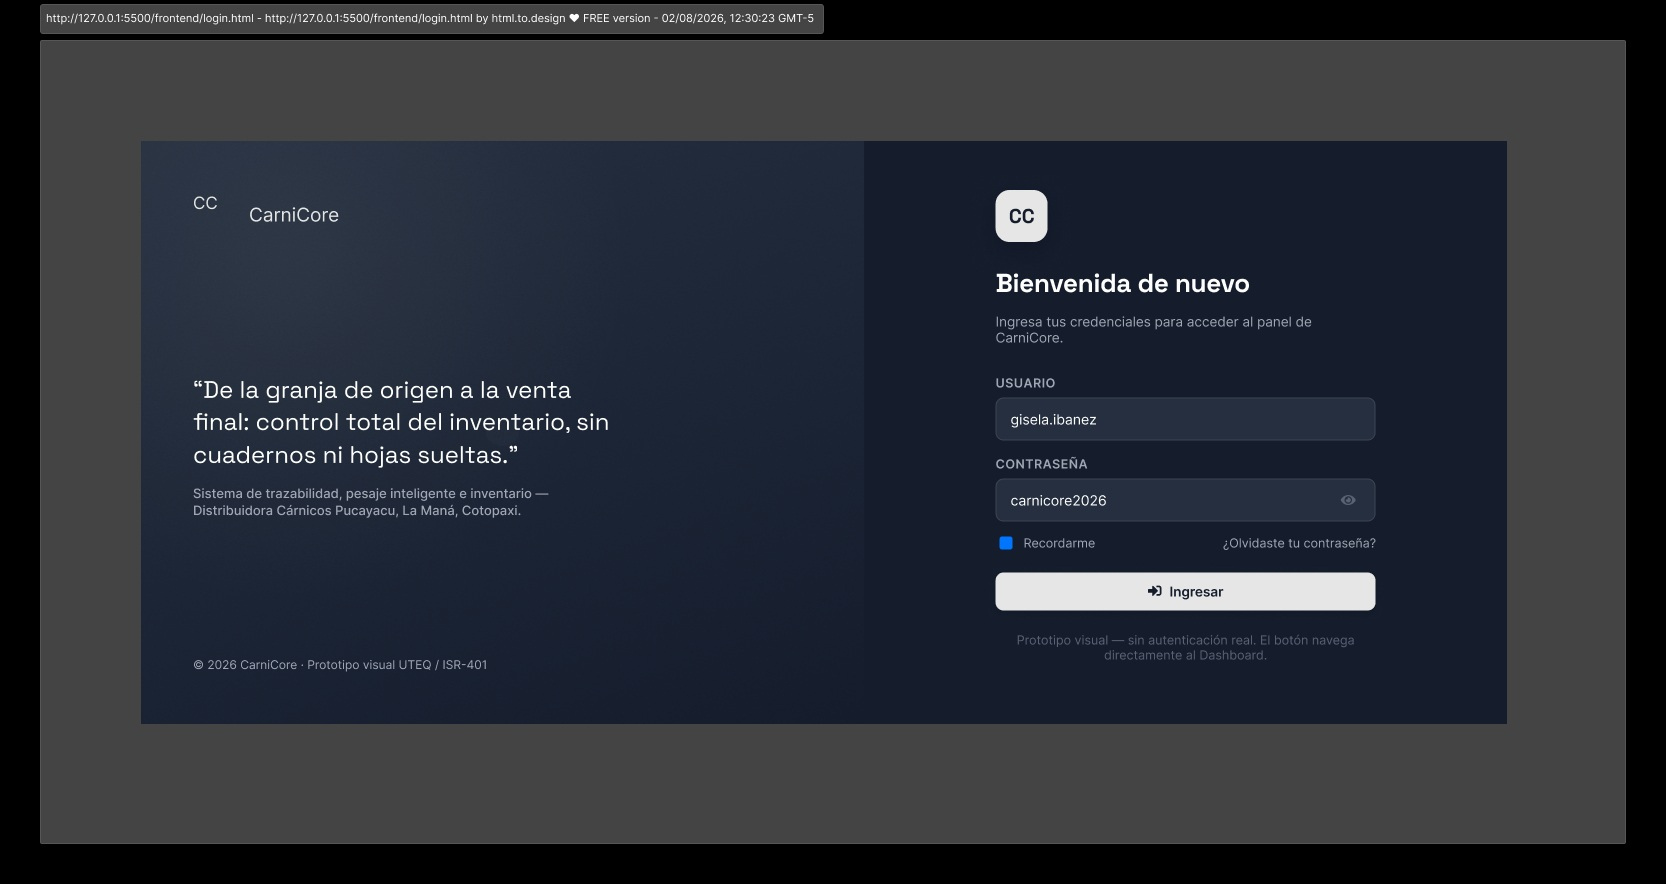
\includegraphics[width=\textwidth,keepaspectratio]{figures/MU-01_login.jpg}
    \caption{MU-01 Interfaz de Login del Sistema}
    \label{fig:diagrama_clases}
\end{figure}

\begin{figure}[H]
    \centering
    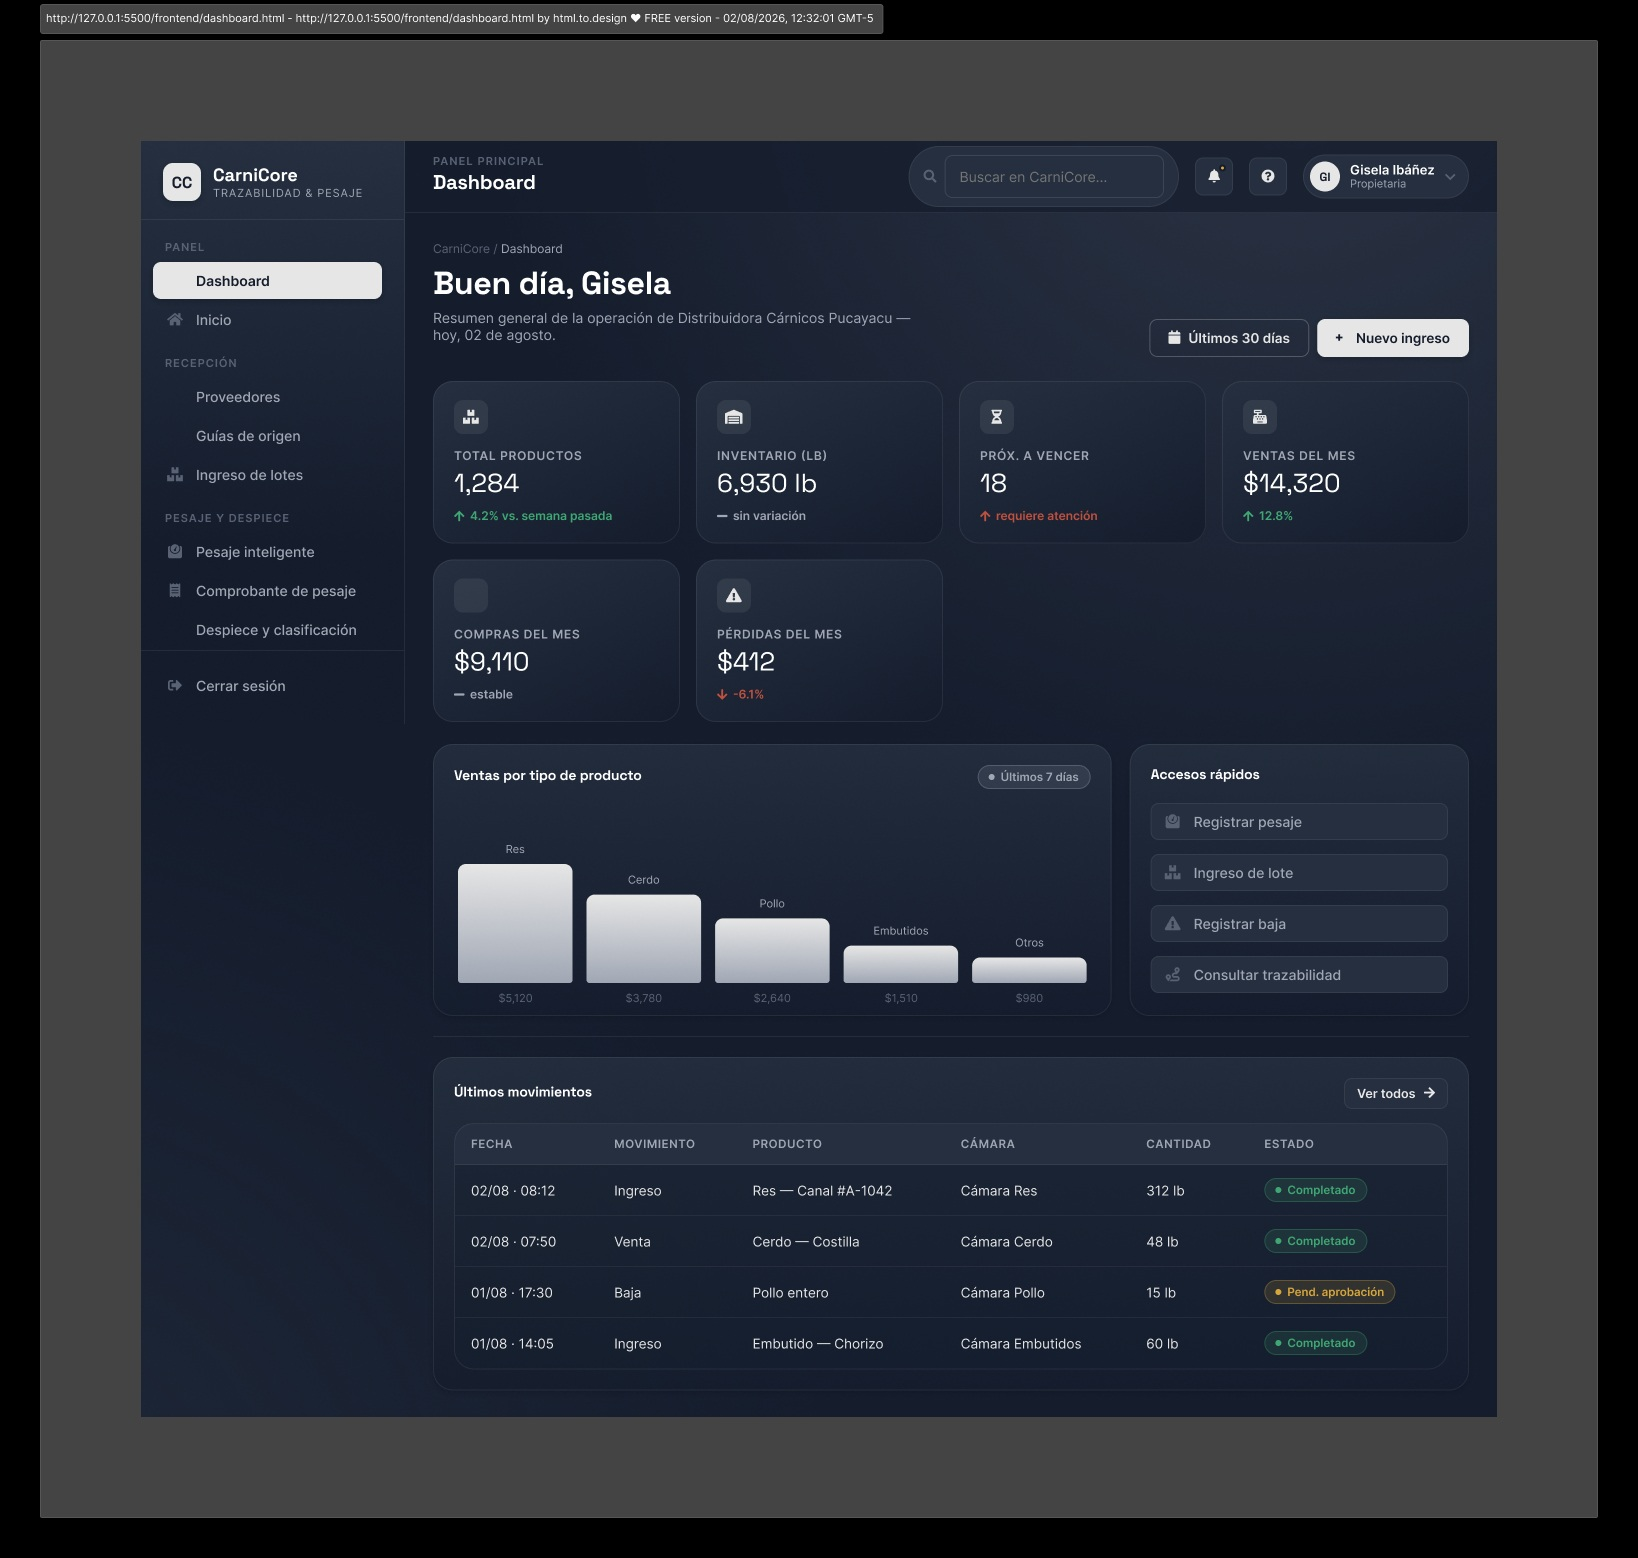
\includegraphics[width=\textwidth,keepaspectratio]{figures/MU-02_dashboard.jpg}
    \caption{MU-02 Interfaz del Dashboard del Sistema}
    \label{fig:diagrama_clases}
\end{figure}

\begin{figure}[H]
    \centering
    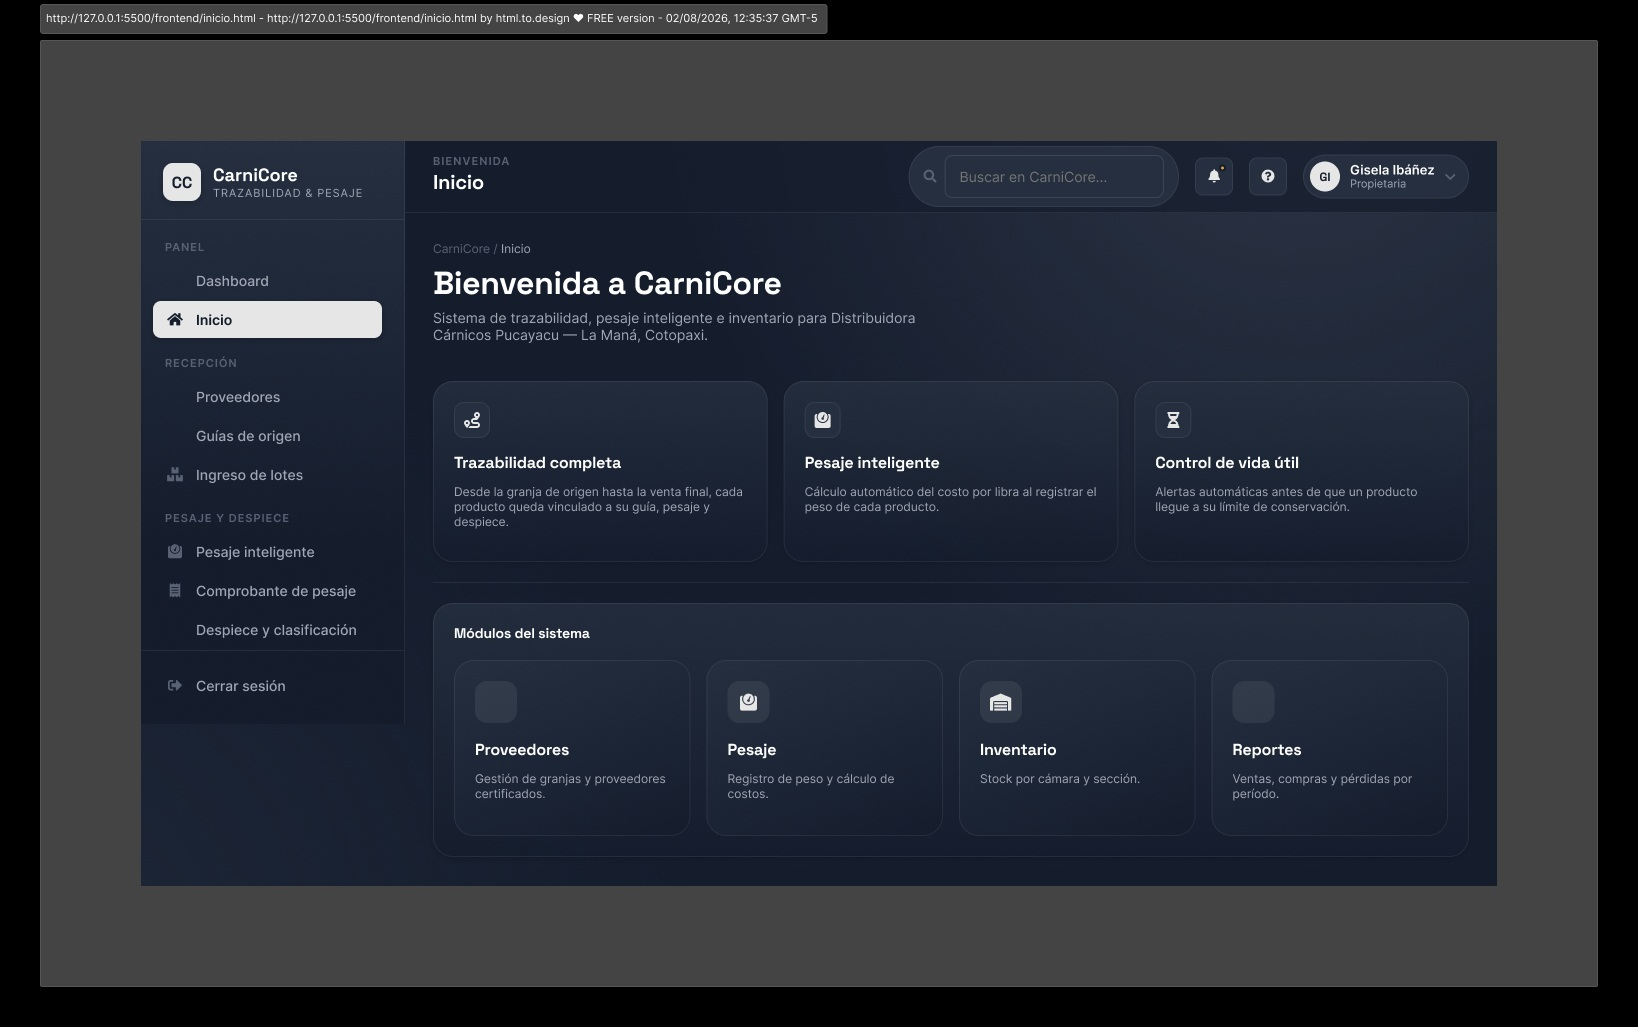
\includegraphics[width=\textwidth,keepaspectratio]{figures/MU-03_inicio.jpg}
    \caption{MU-03 Interfaz de pantalla de inicio del Sistema}
    \label{fig:diagrama_clases}
\end{figure}

\begin{figure}[H]
    \centering
    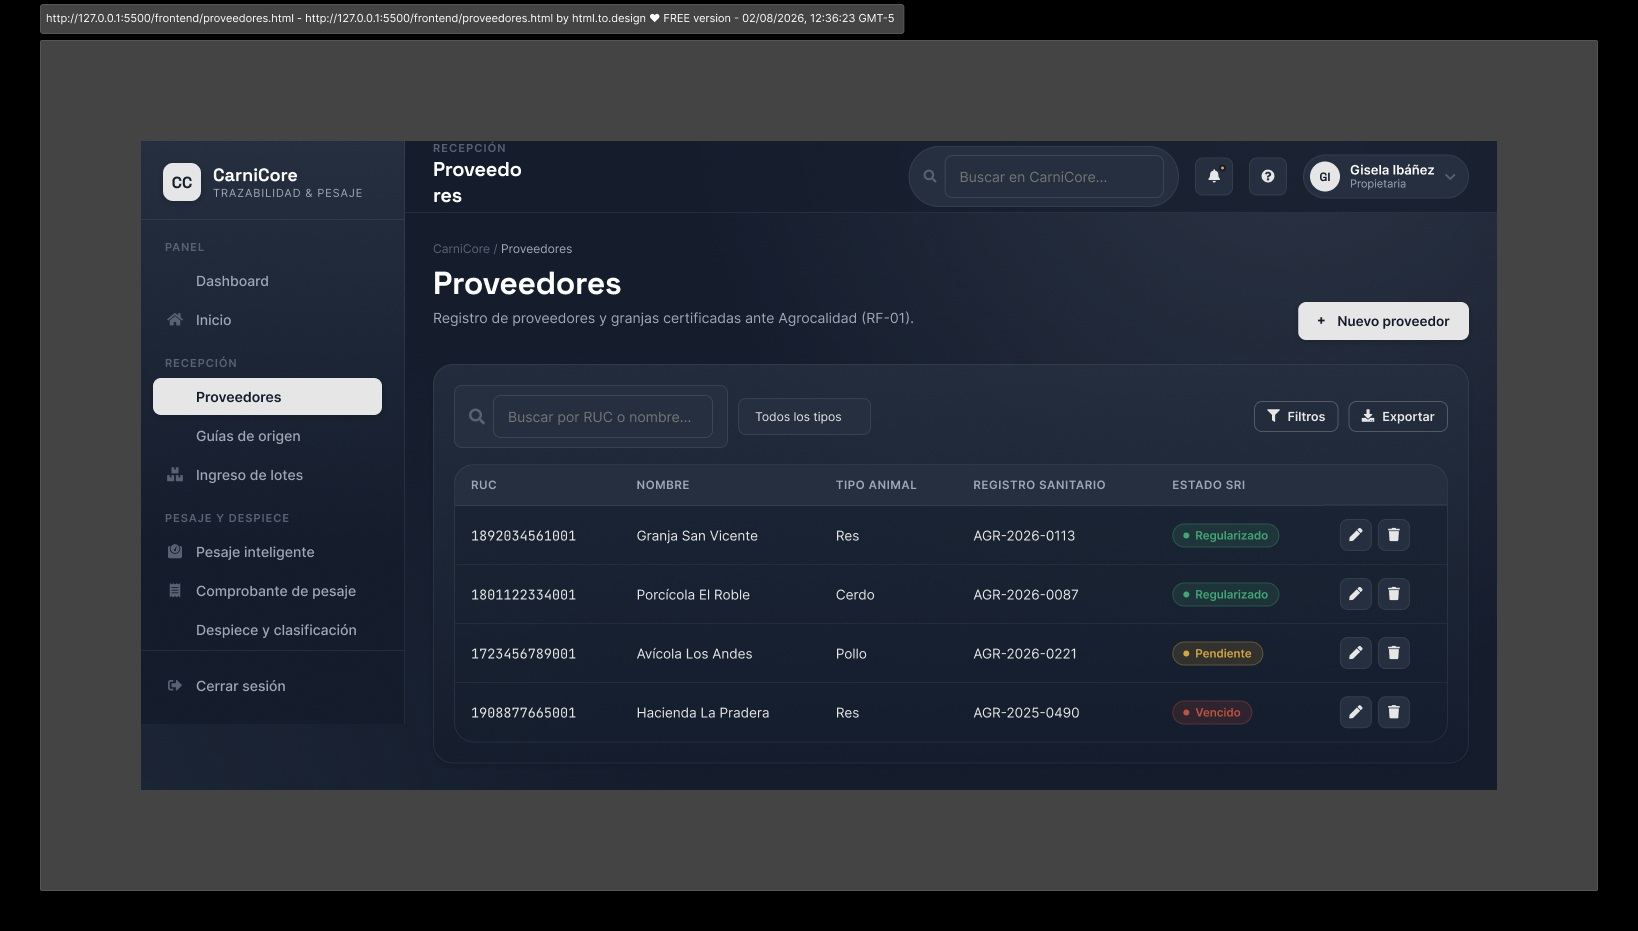
\includegraphics[width=\textwidth,keepaspectratio]{figures/MU-04_proveedores.jpg}
    \caption{MU-04 Interfaz del módulo de proveedores del Sistema}
    \label{fig:diagrama_clases}
\end{figure}

\begin{figure}[H]
    \centering
    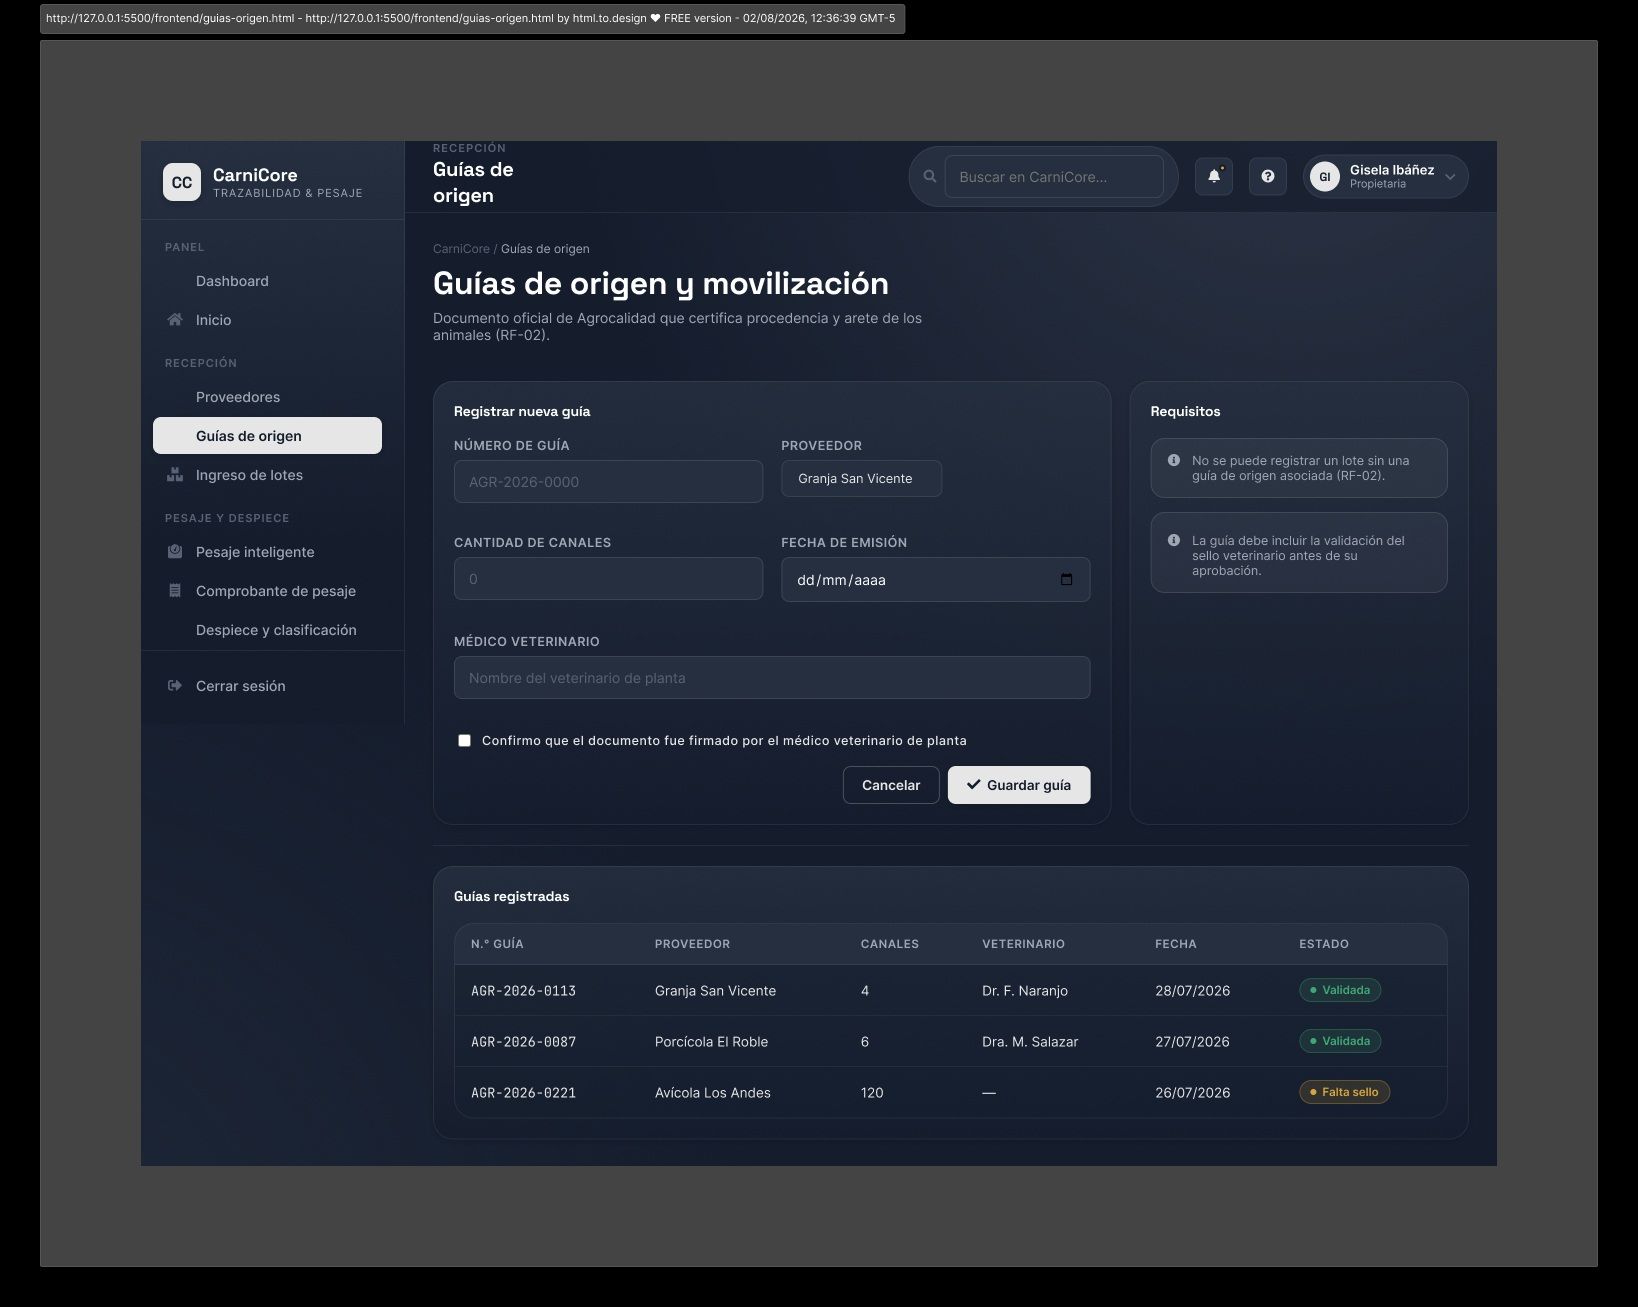
\includegraphics[width=\textwidth,keepaspectratio]{figures/MU-05_guias_origen.jpg}
    \caption{MU-05 Interfaz del módulo de guías de origen del Sistema}
    \label{fig:diagrama_clases}
\end{figure}

\begin{figure}[H]
    \centering
    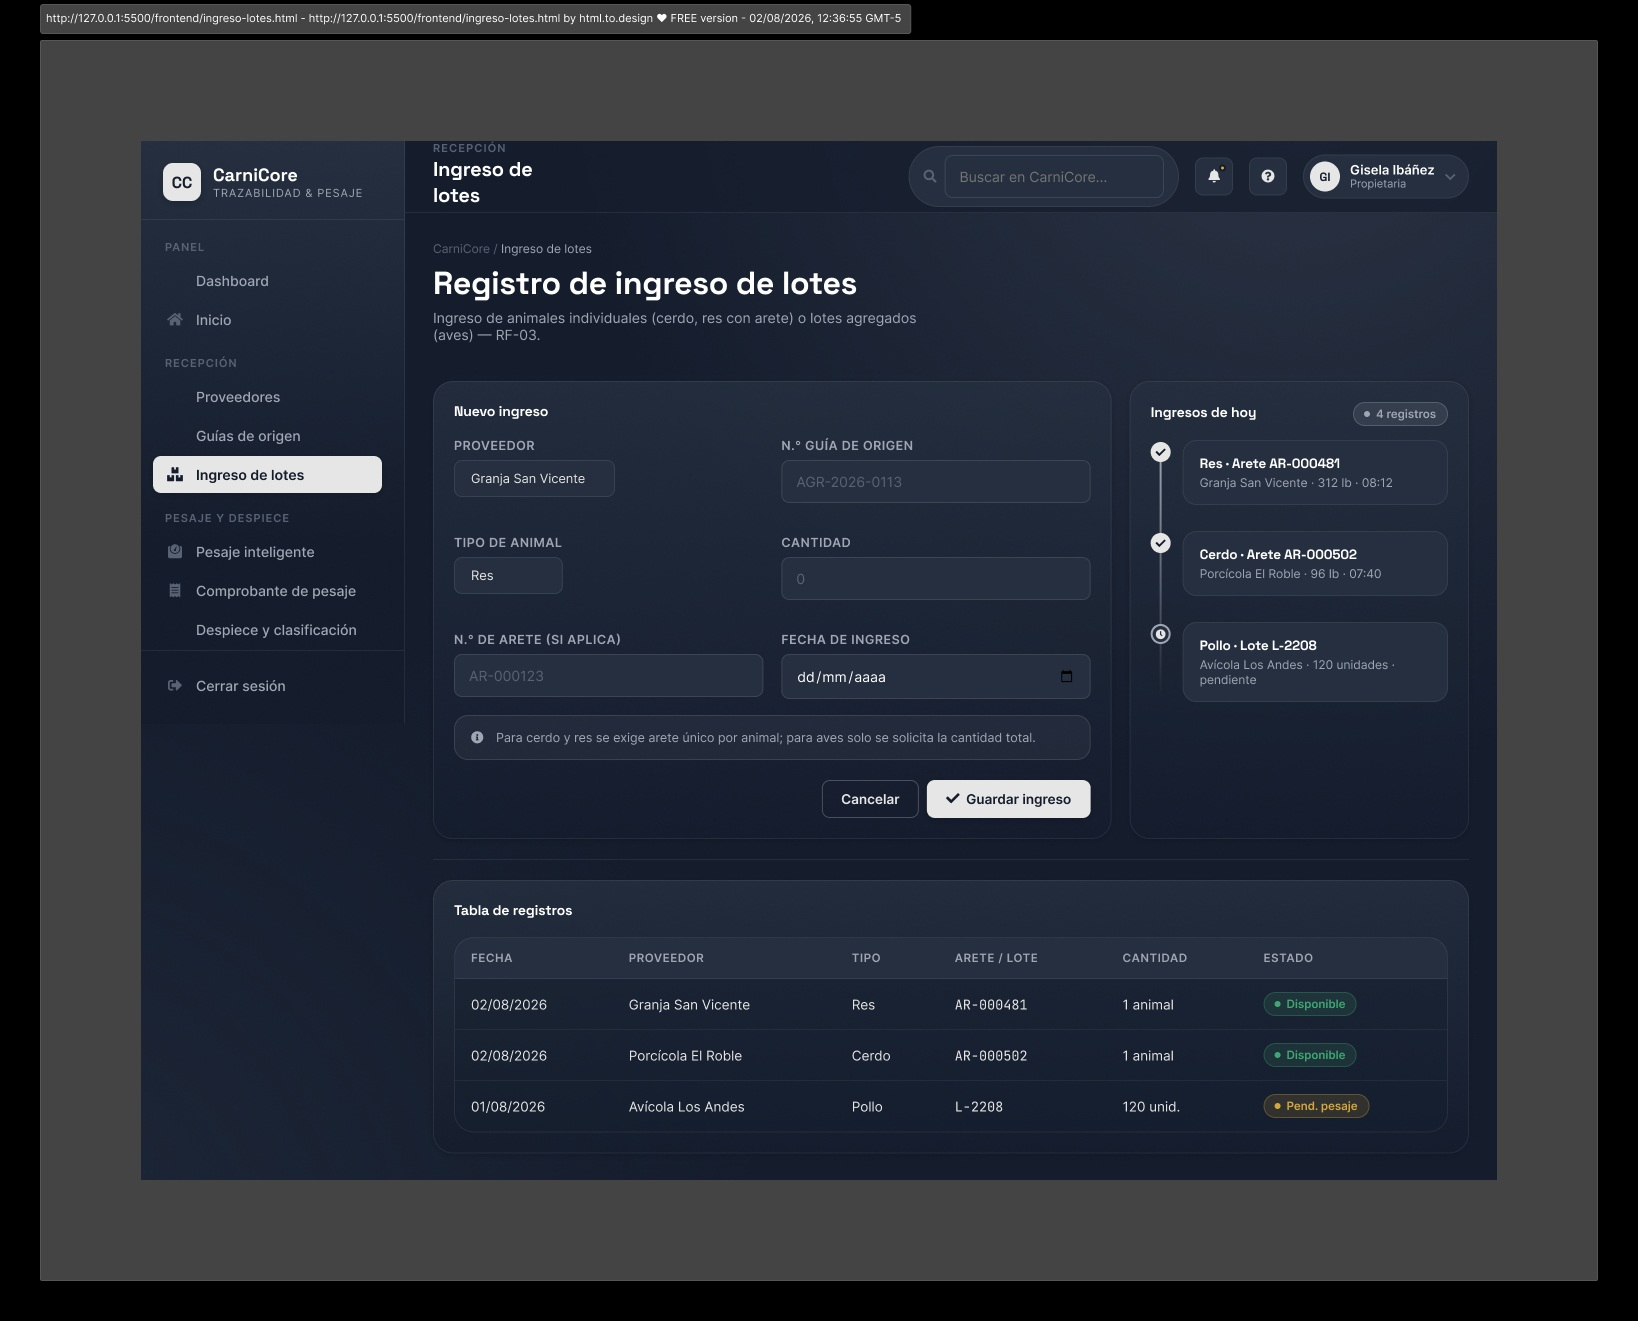
\includegraphics[width=\textwidth,keepaspectratio]{figures/MU-06_ingreso_lotes.jpg}
    \caption{MU-06 Interfaz del módulo de ingreso de lotes del Sistema}
    \label{fig:diagrama_clases}
\end{figure}

\begin{figure}[H]
    \centering
    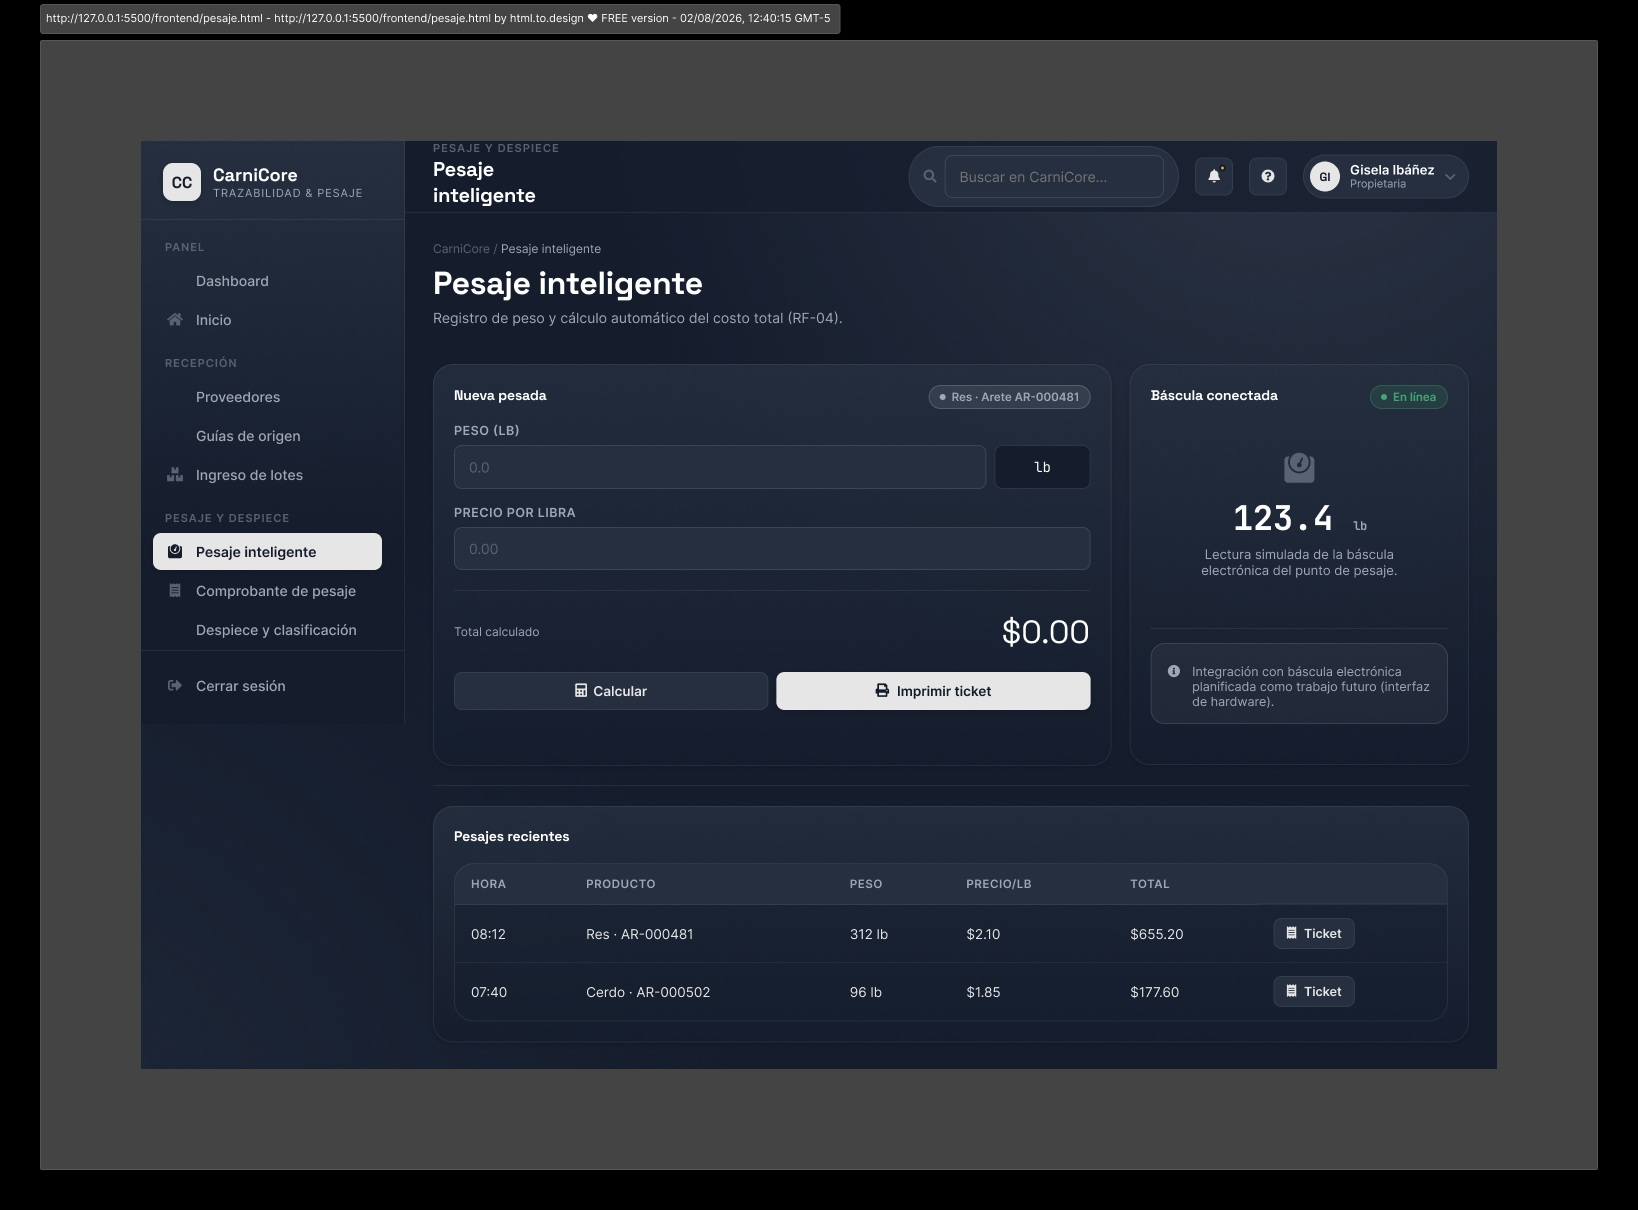
\includegraphics[width=\textwidth,keepaspectratio]{figures/MU-07_pesaje_inteligente.jpg}
    \caption{MU-07 Interfaz del módulo de pesaje inteligente del Sistema}
    \label{fig:diagrama_clases}
\end{figure}

\begin{figure}[H]
    \centering
    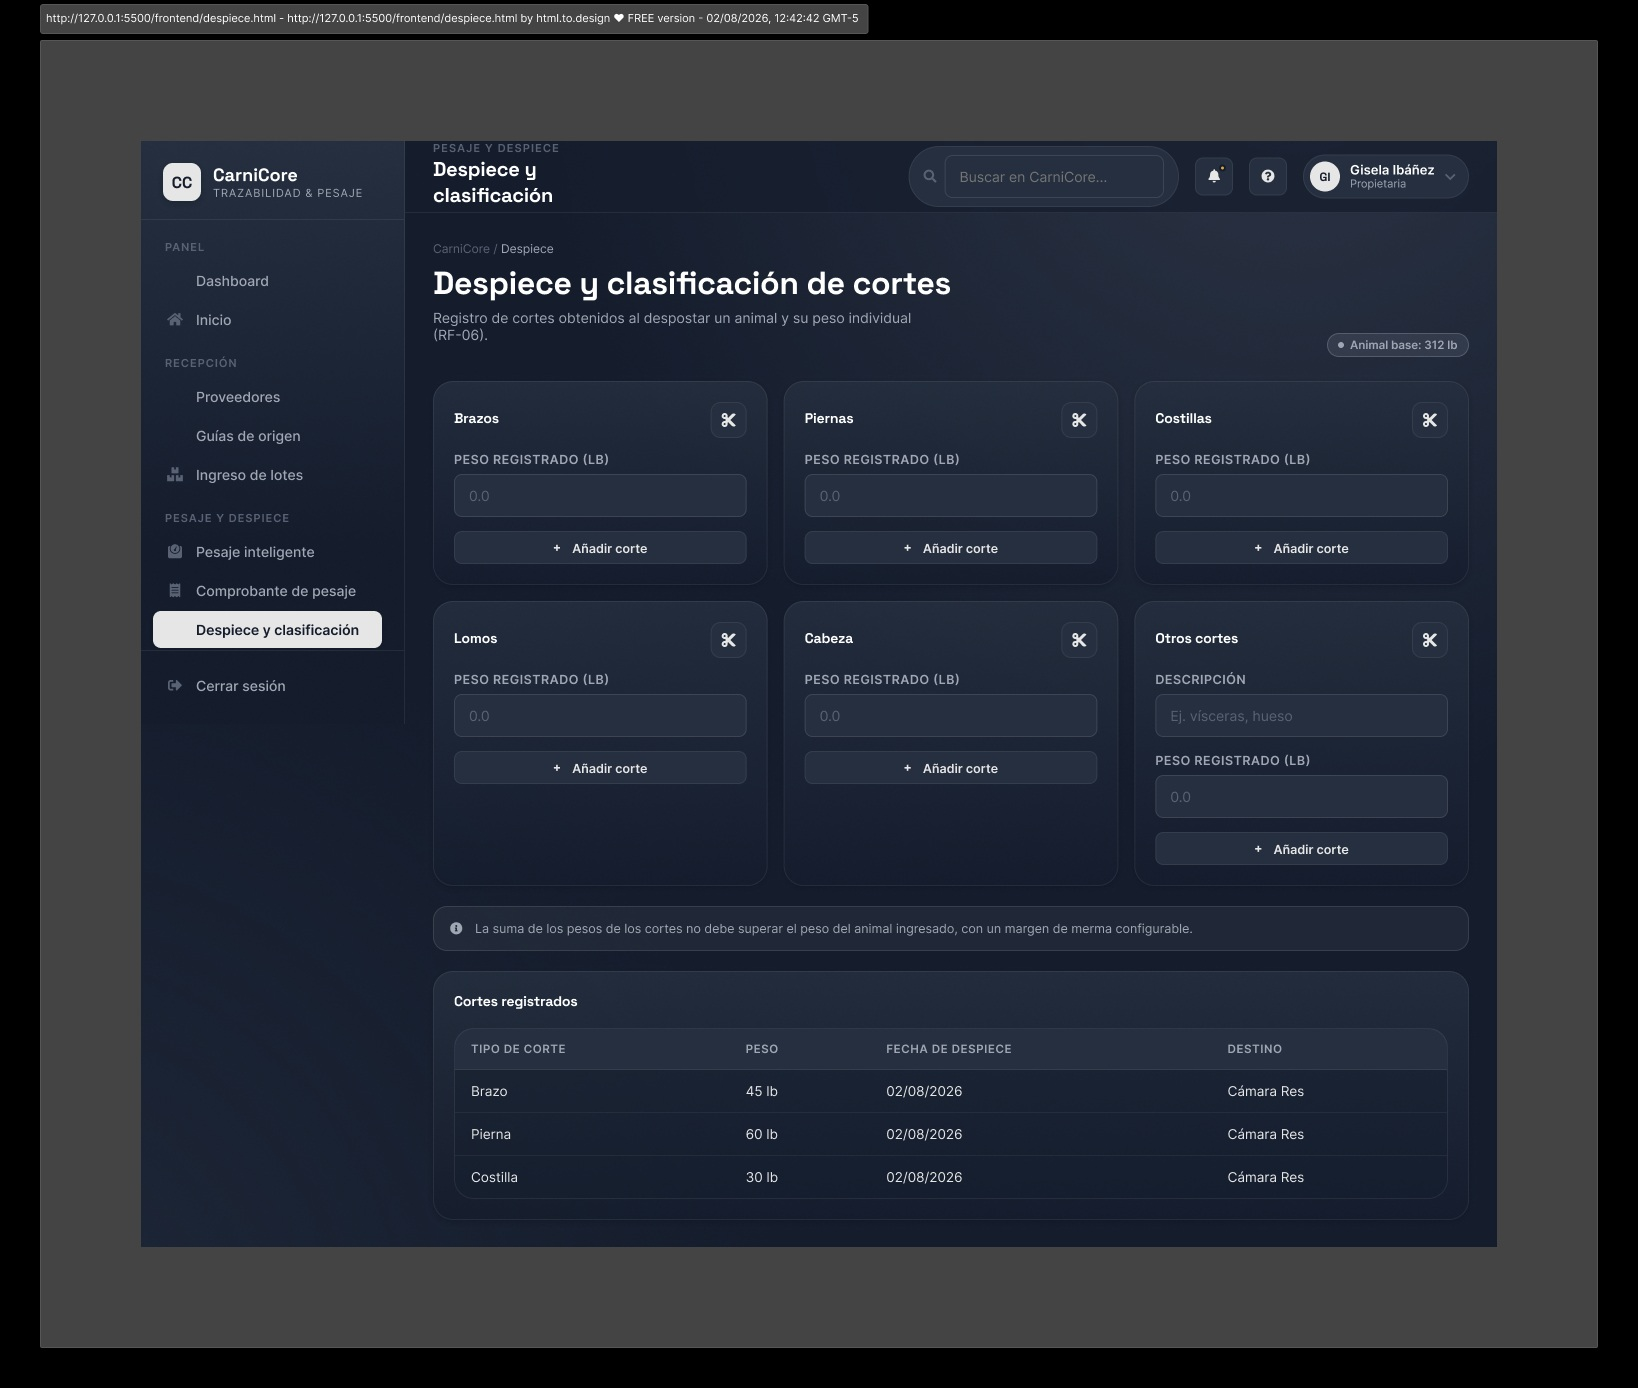
\includegraphics[width=\textwidth,keepaspectratio]{figures/MU-08_despiece.jpg}
    \caption{MU-08 Interfaz del módulo de despiece del Sistema}
    \label{fig:diagrama_clases}
\end{figure}

\begin{figure}[H]
    \centering
    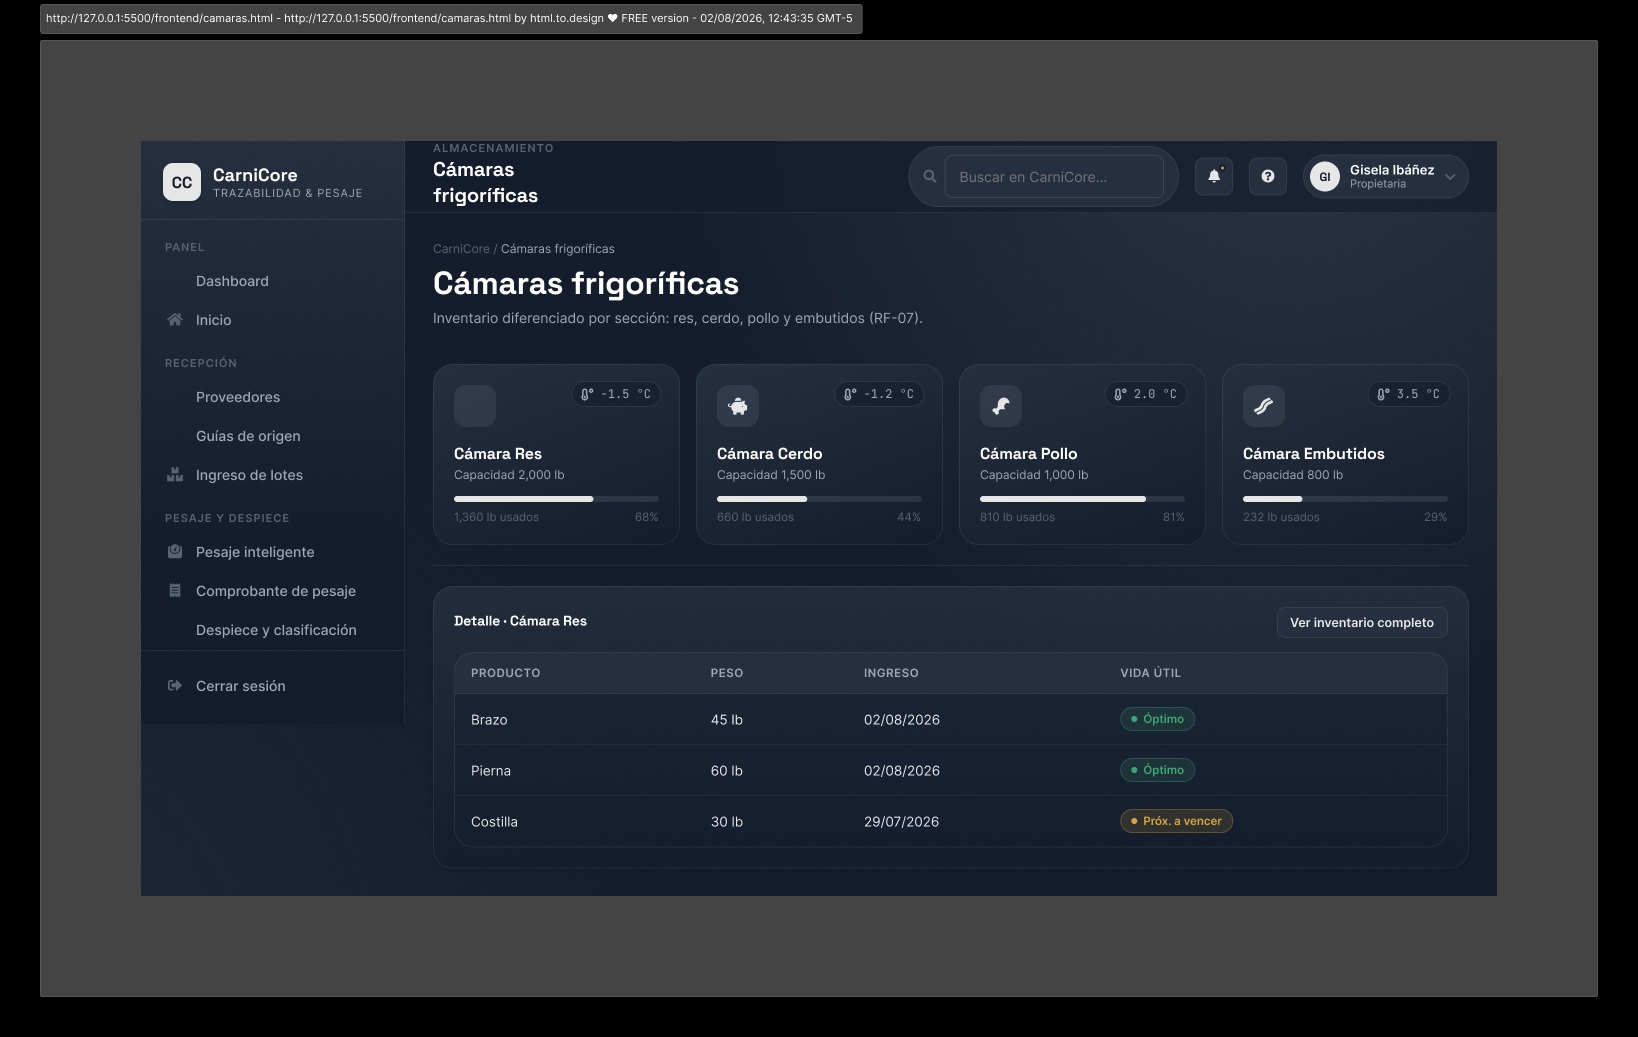
\includegraphics[width=\textwidth,keepaspectratio]{figures/MU-09_camaras_frigorificas.jpg}
    \caption{MU-09 Interfaz del módulo de guías de origen del Sistema}
    \label{fig:diagrama_clases}
\end{figure}

\begin{figure}[H]
    \centering
    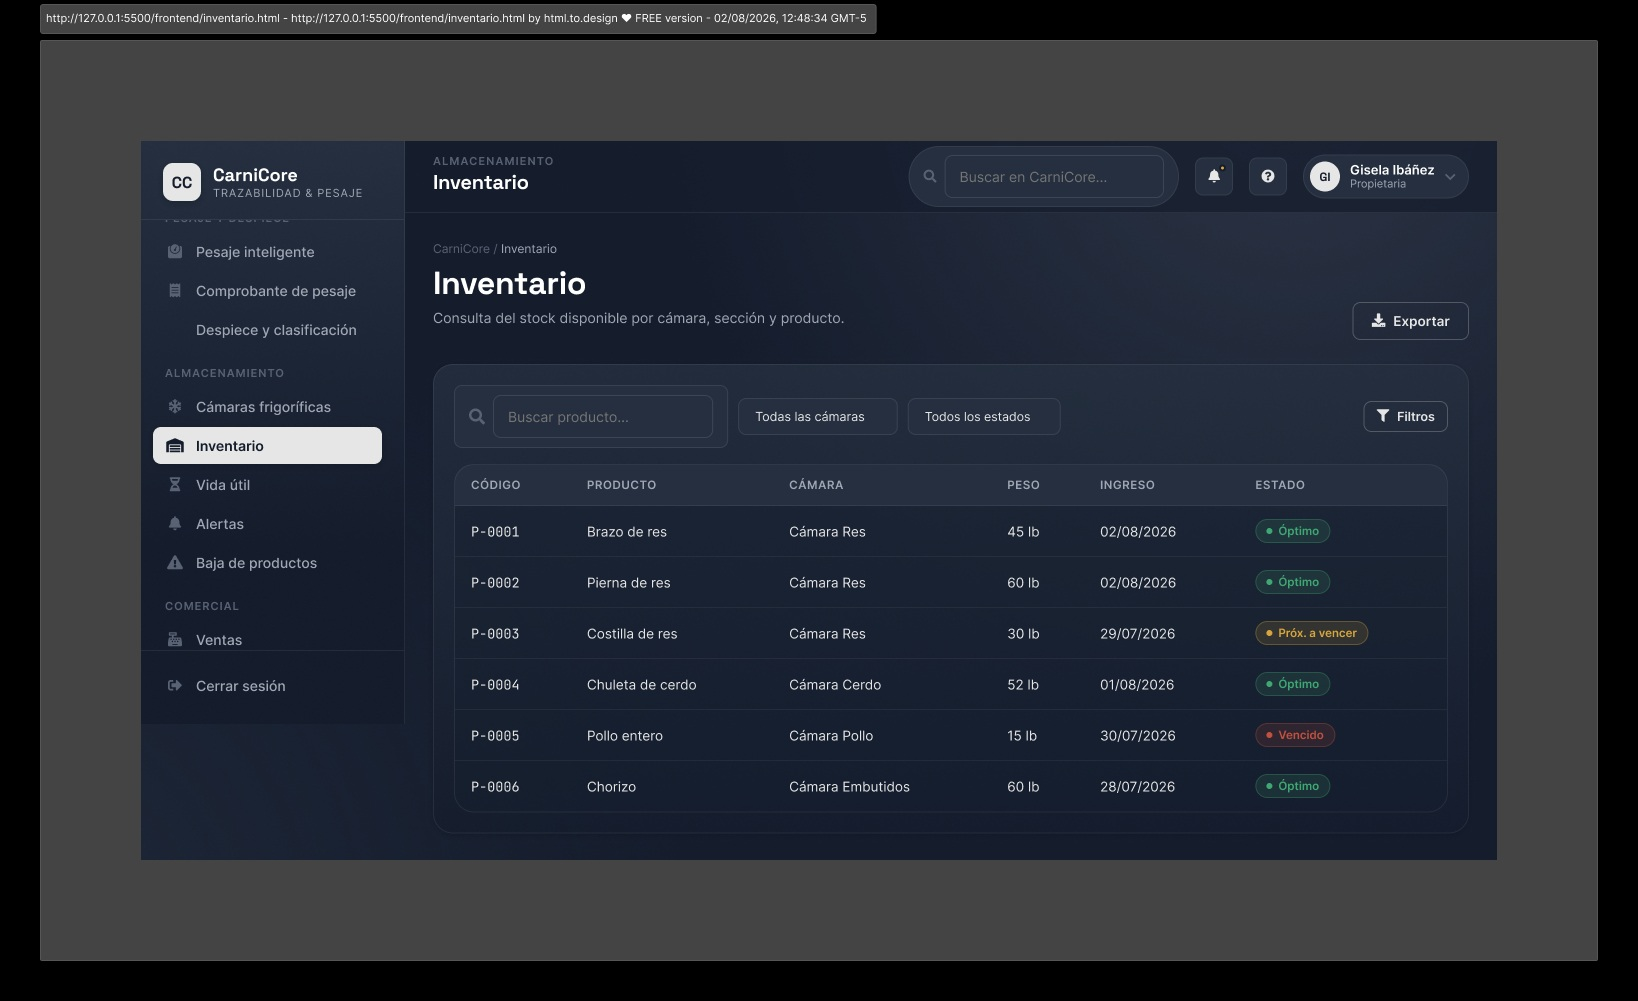
\includegraphics[width=\textwidth,keepaspectratio]{figures/MU-10_inventario.jpg}
    \caption{MU-10 Interfaz del módulo de inventarios del Sistema}
    \label{fig:diagrama_clases}
\end{figure}

\begin{figure}[H]
    \centering
    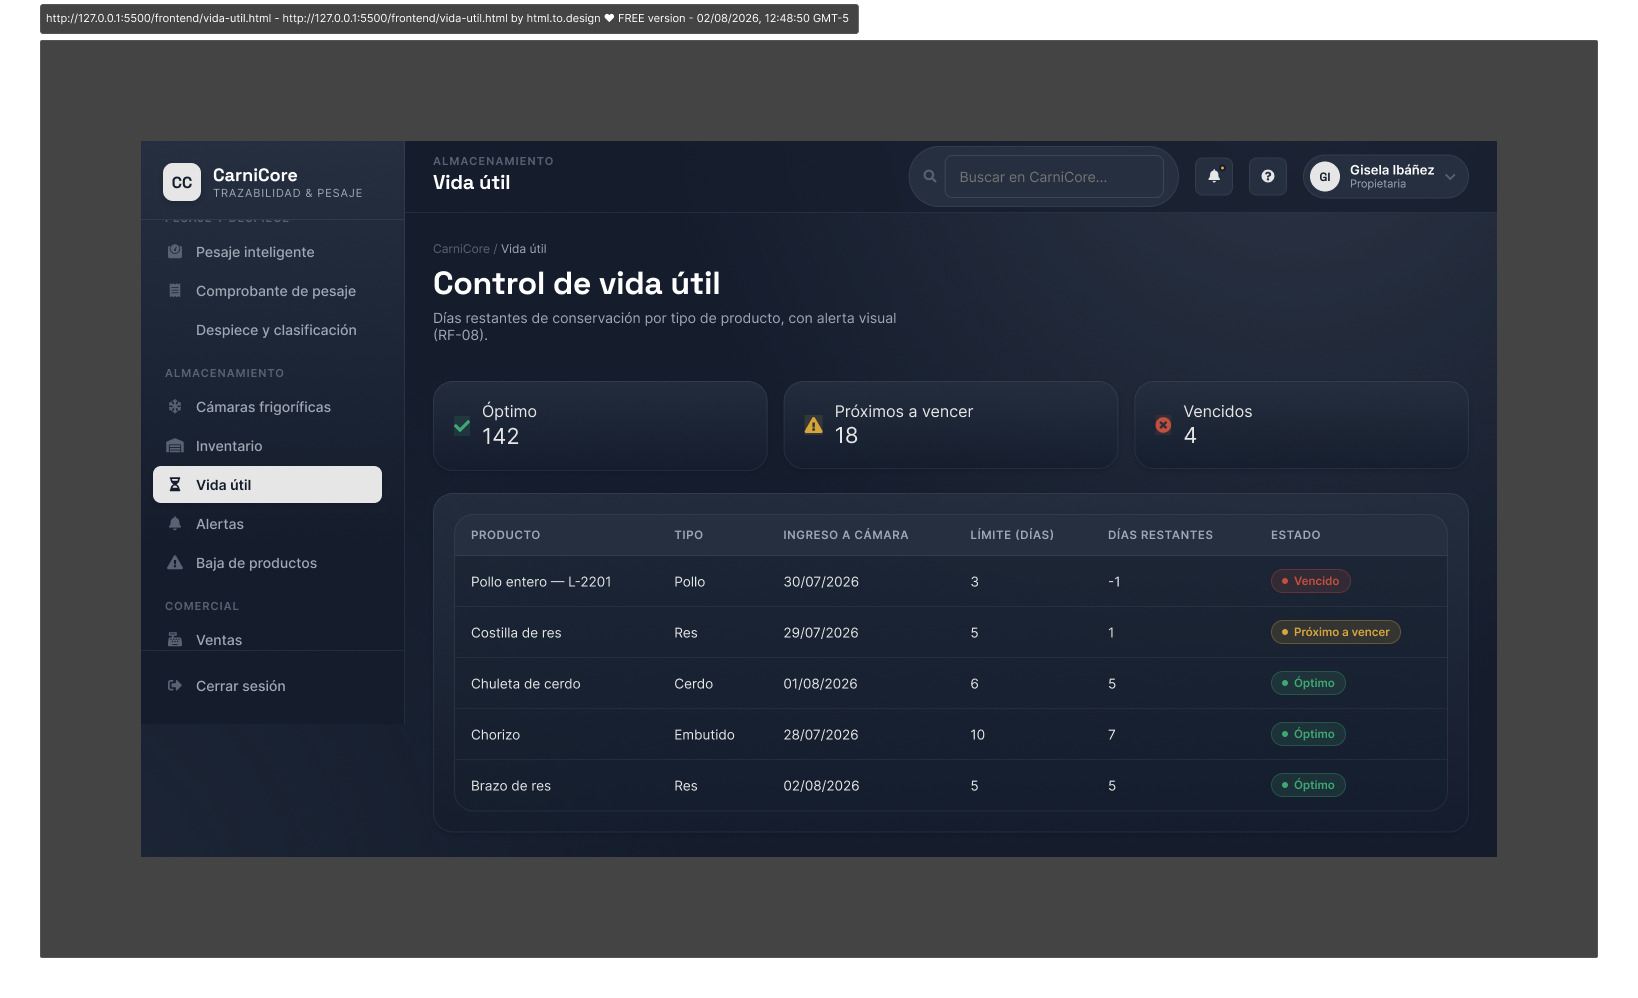
\includegraphics[width=\textwidth,keepaspectratio]{figures/MU-11_vida_util.jpg}
    \caption{MU-11 Interfaz del módulo de vida útil del Sistema}
    \label{fig:diagrama_clases}
\end{figure}

\begin{figure}[H]
    \centering
    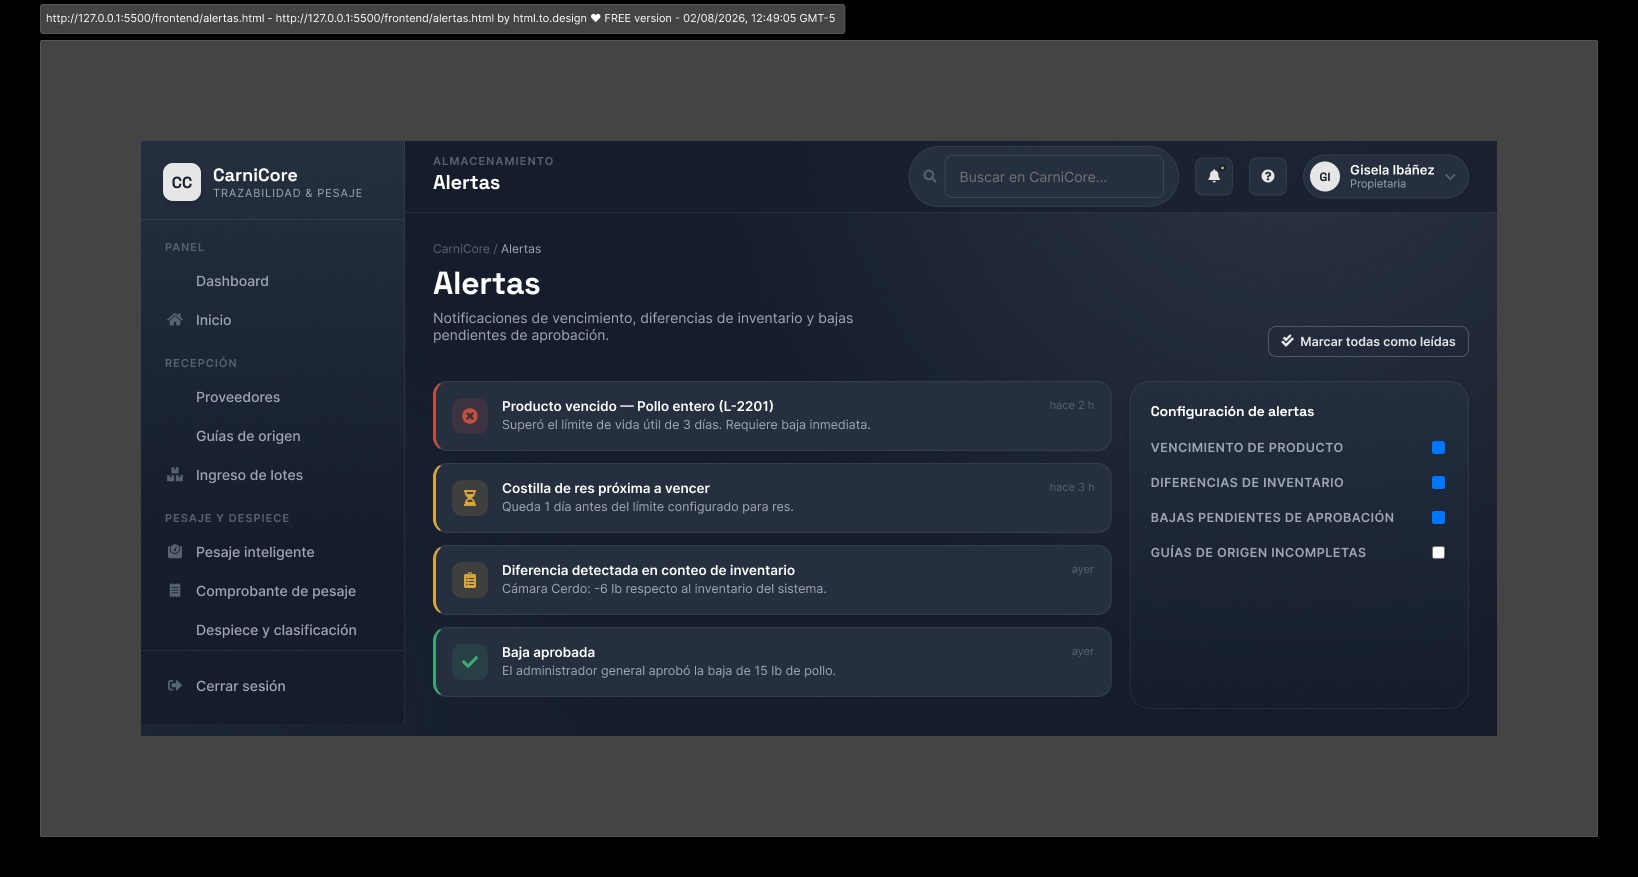
\includegraphics[width=\textwidth,keepaspectratio]{figures/MU-12_alertas.jpg}
    \caption{MU-12 Interfaz del módulo de alertas del Sistema}
    \label{fig:diagrama_clases}
\end{figure}

\begin{figure}[H]
    \centering
    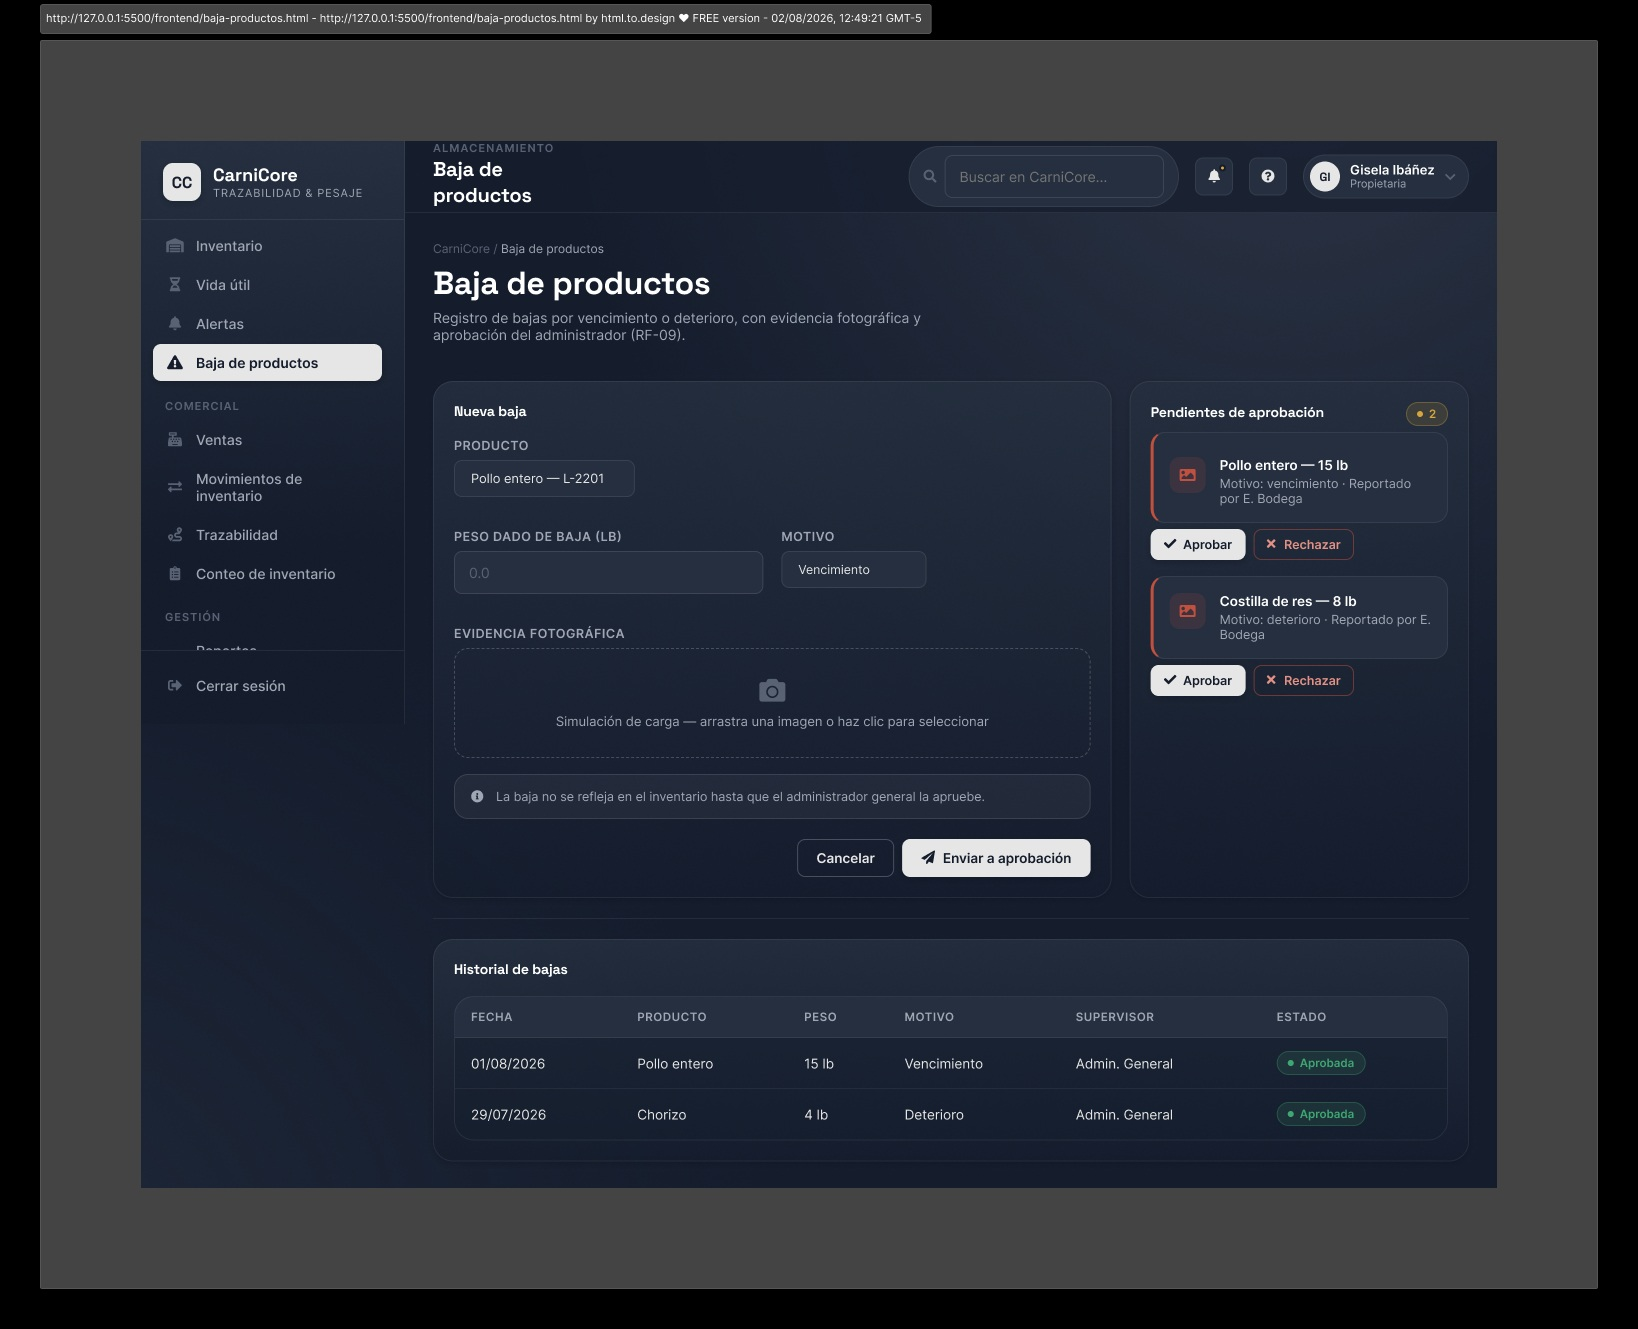
\includegraphics[width=\textwidth,keepaspectratio]{figures/MU-13_baja_productos.jpg}
    \caption{MU-13 Interfaz del módulo de baja de productos del Sistema}
    \label{fig:diagrama_clases}
\end{figure}

\begin{figure}[H]
    \centering
    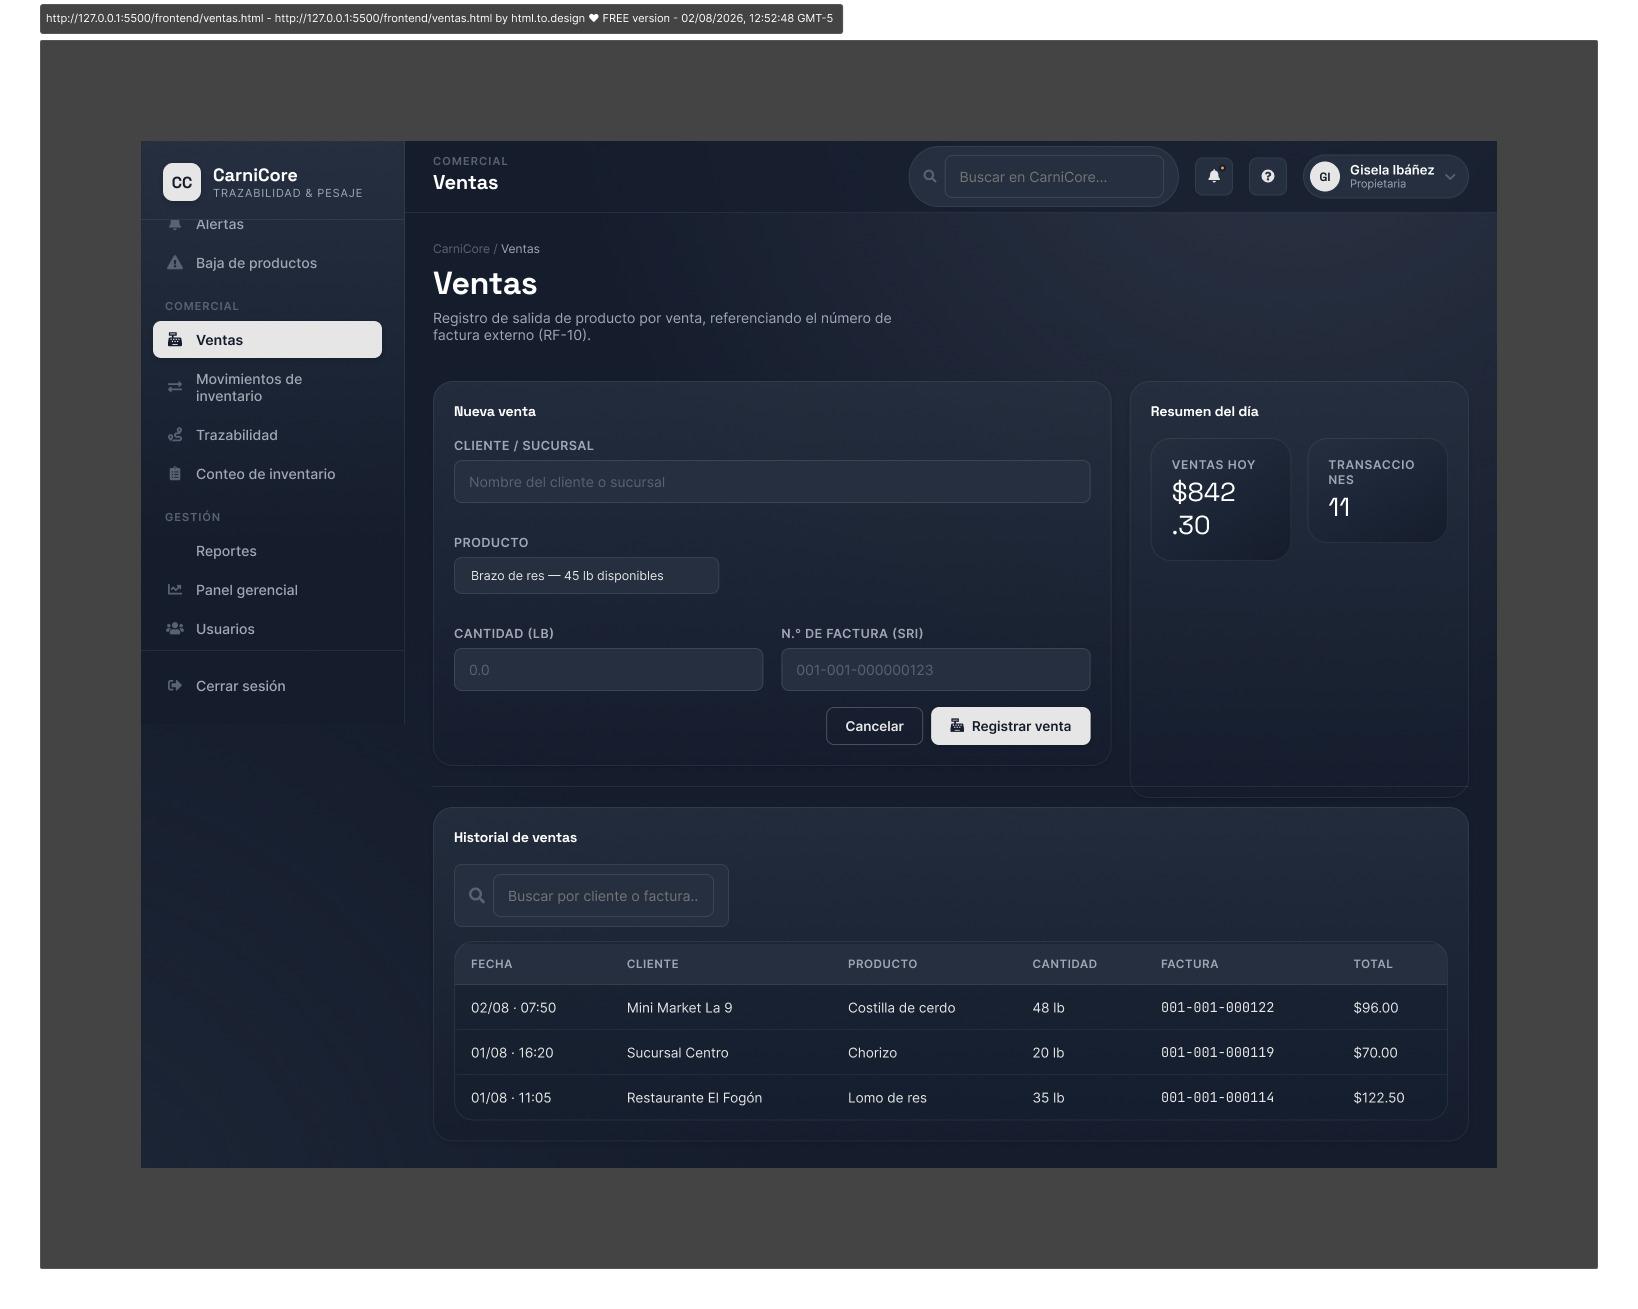
\includegraphics[width=\textwidth,keepaspectratio]{figures/MU-14_ventas.jpg}
    \caption{MU-14 Interfaz del módulo de ventas del Sistema}
    \label{fig:diagrama_clases}
\end{figure}

\begin{figure}[H]
    \centering
    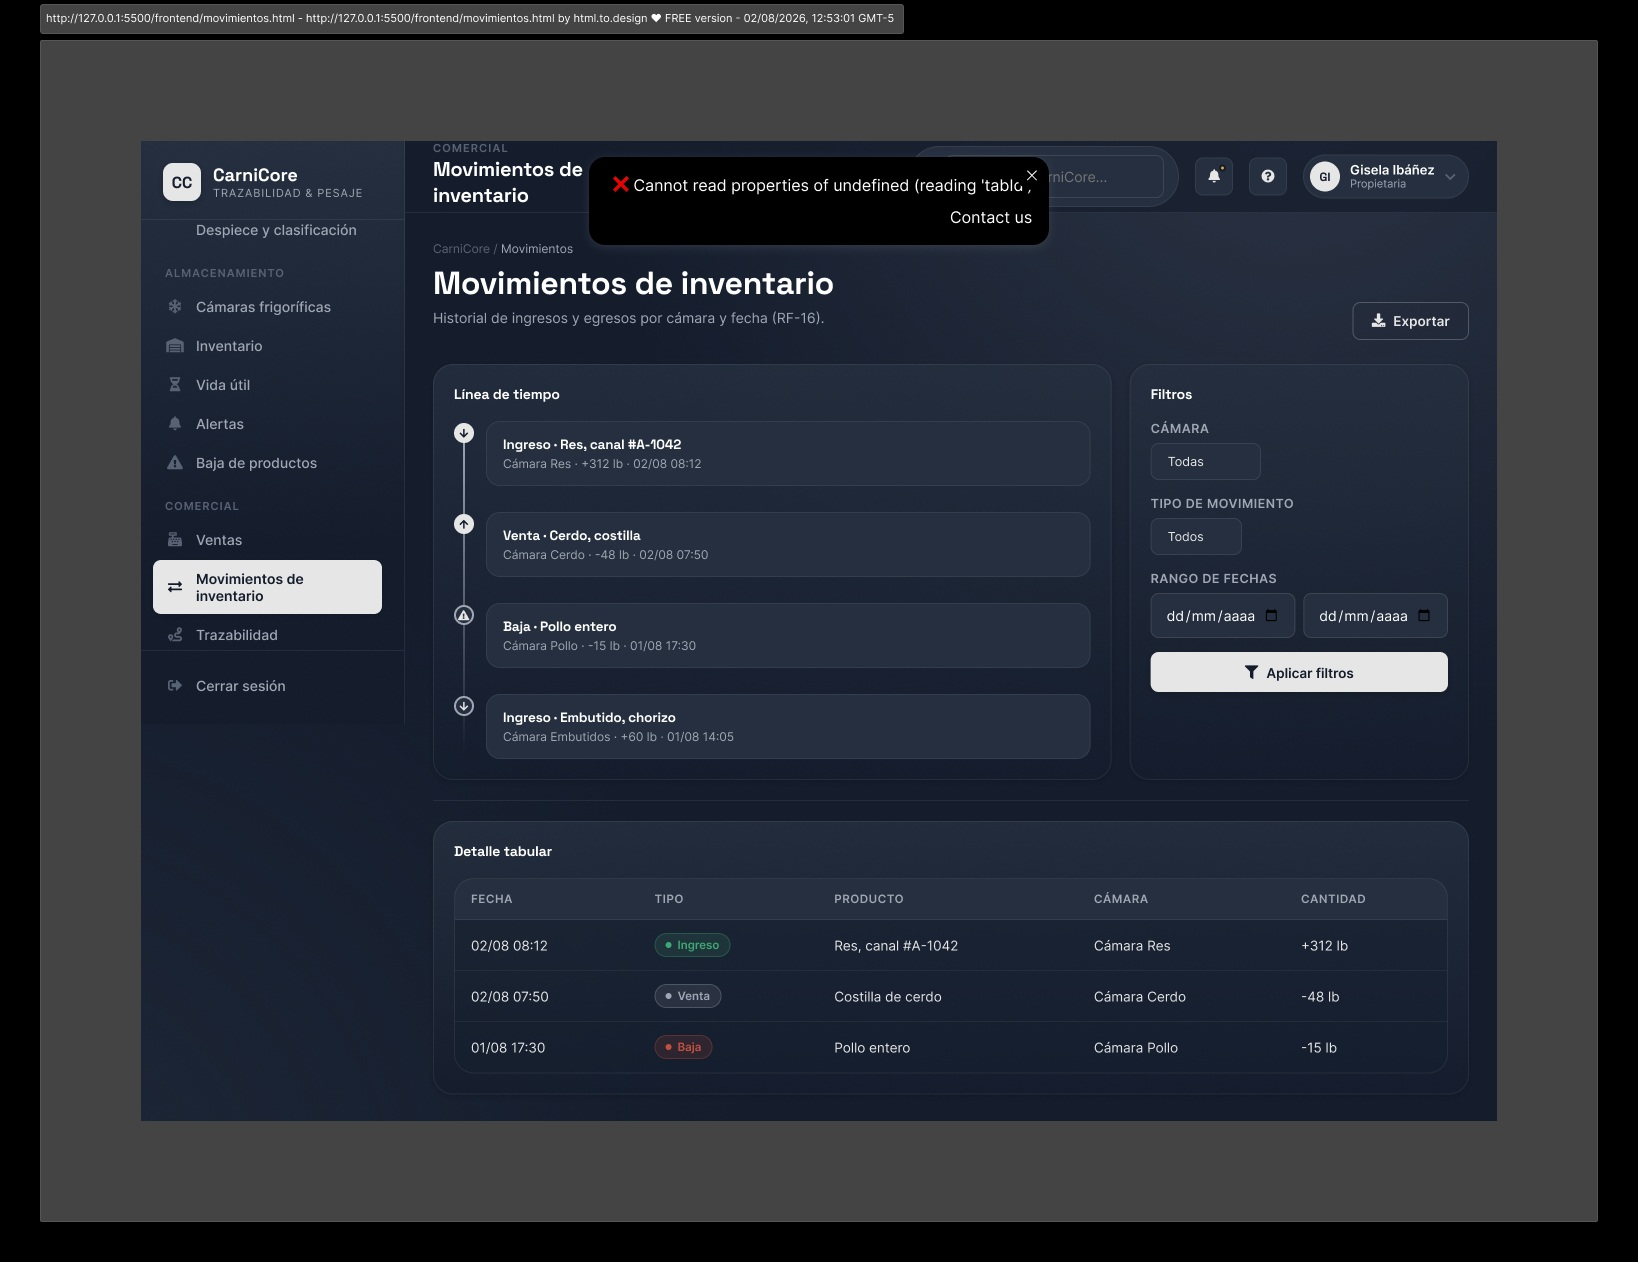
\includegraphics[width=\textwidth,keepaspectratio]{figures/MU-15_movimientos_inventario.jpg}
    \caption{MU-15 Interfaz del módulo de movimientos de inventario del Sistema}
    \label{fig:diagrama_clases}
\end{figure}

\begin{figure}[H]
    \centering
    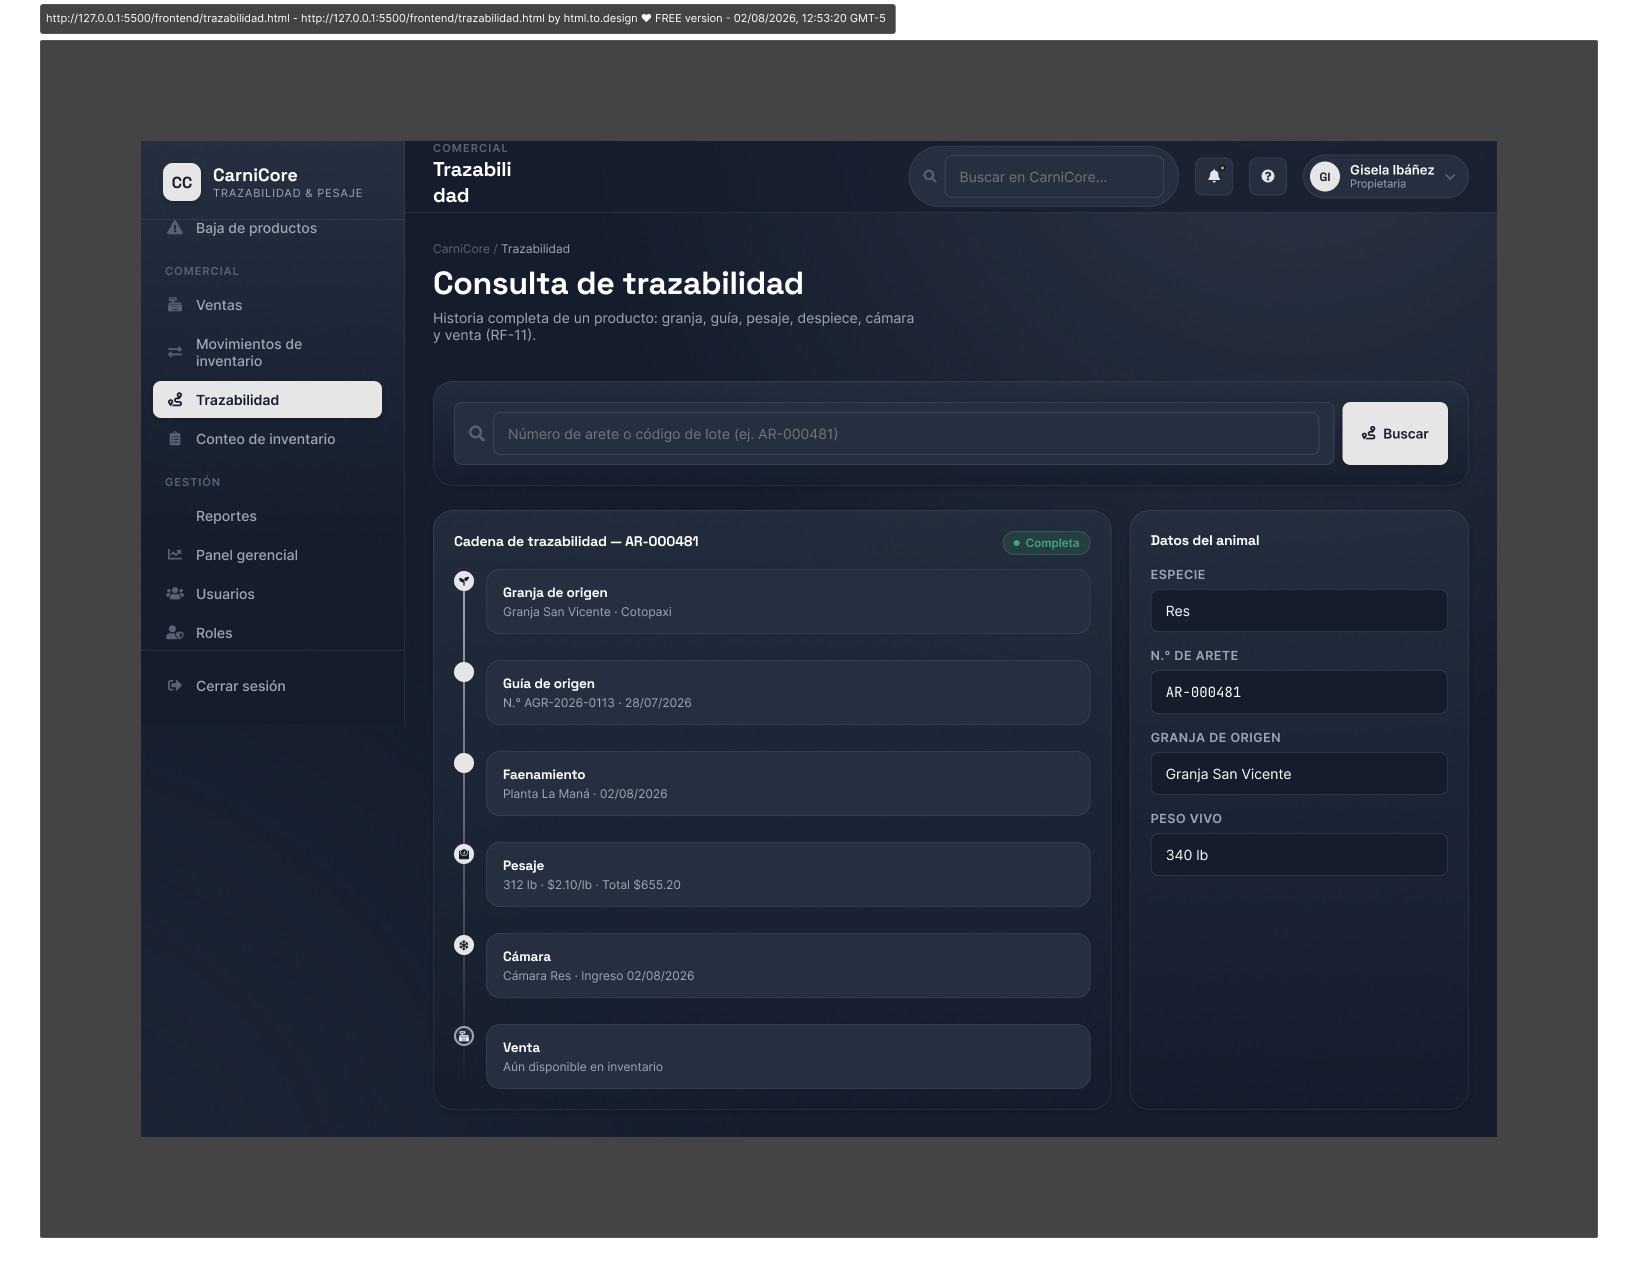
\includegraphics[width=\textwidth,keepaspectratio]{figures/MU-16_trazabilidad.jpg}
    \caption{MU-16 Interfaz del módulo de trazabilidad del Sistema}
    \label{fig:diagrama_clases}
\end{figure}

\begin{figure}[H]
    \centering
    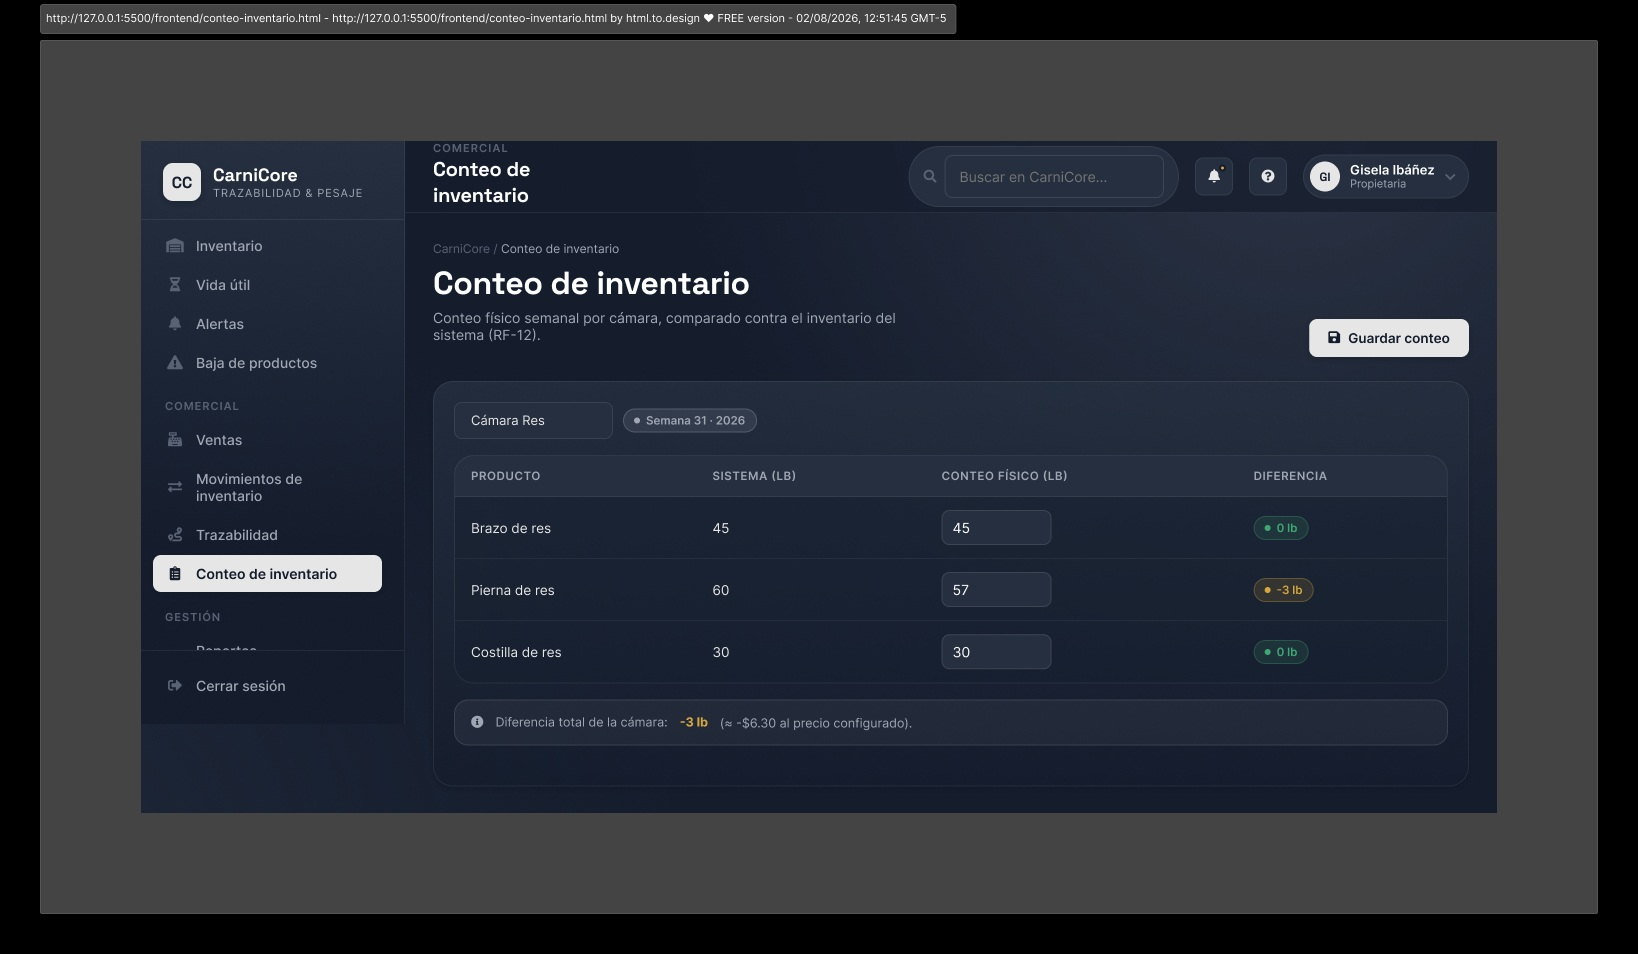
\includegraphics[width=\textwidth,keepaspectratio]{figures/MU-17_conteo_inventario.jpg}
    \caption{MU-17 Interfaz del módulo de conteo de inventario del Sistema}
    \label{fig:diagrama_clases}
\end{figure}

\begin{figure}[H]
    \centering
    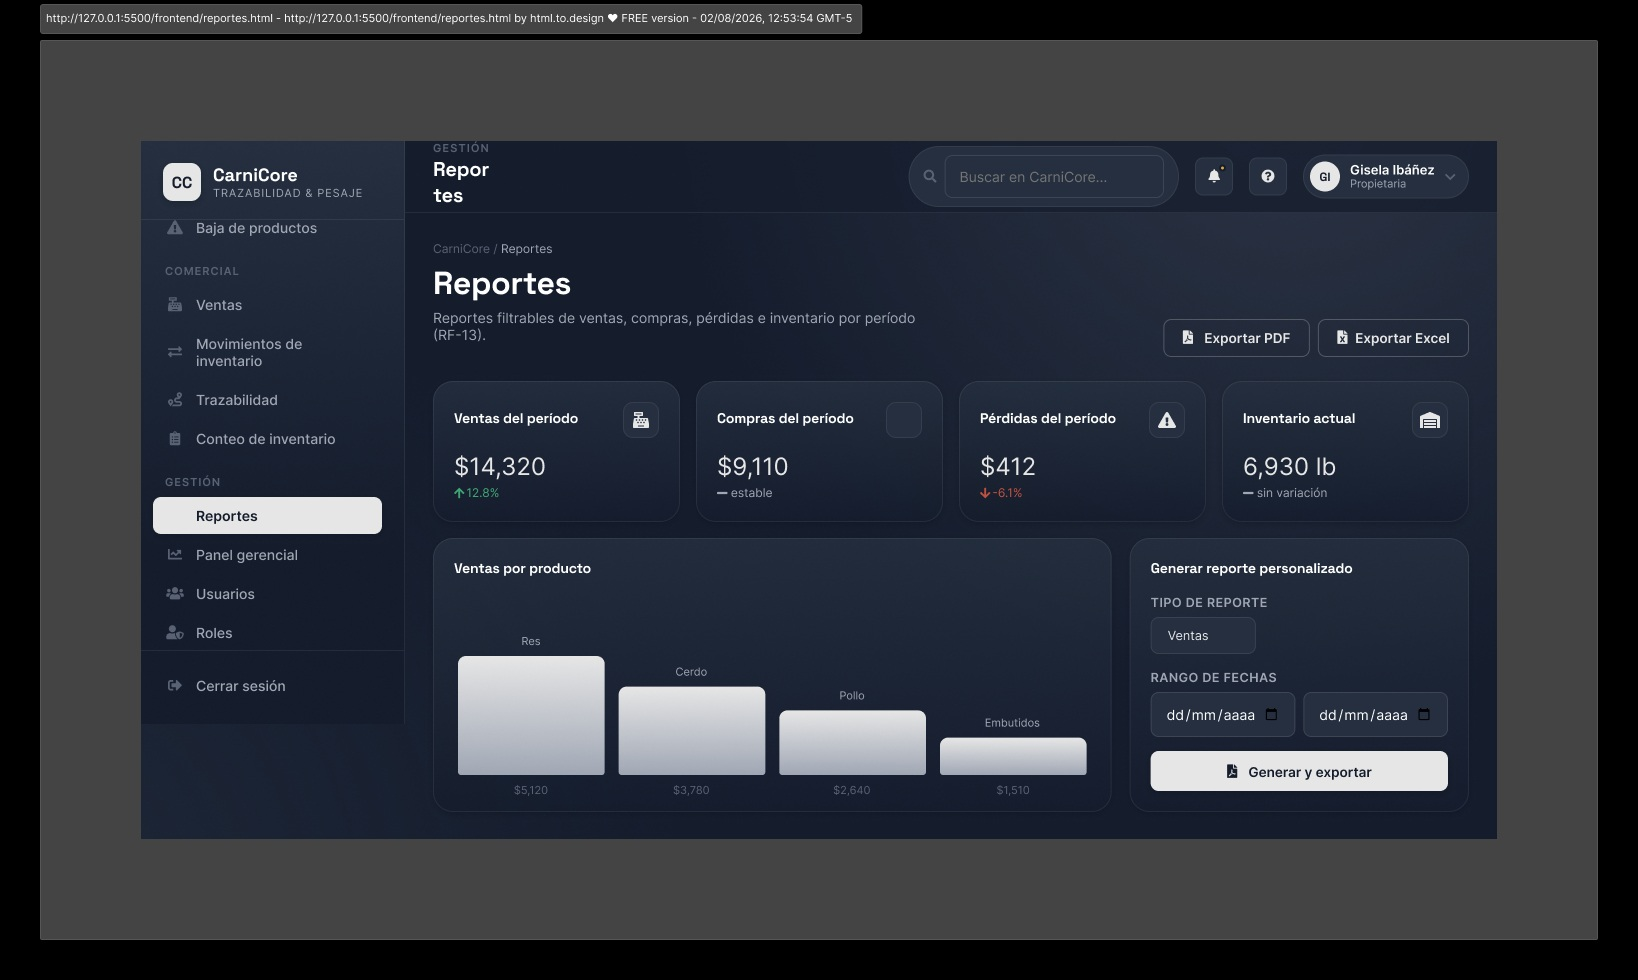
\includegraphics[width=\textwidth,keepaspectratio]{figures/MU-18_reportes.jpg}
    \caption{MU-18 Interfaz del módulo de reportes del Sistema}
    \label{fig:diagrama_clases}
\end{figure}

\begin{figure}[H]
    \centering
    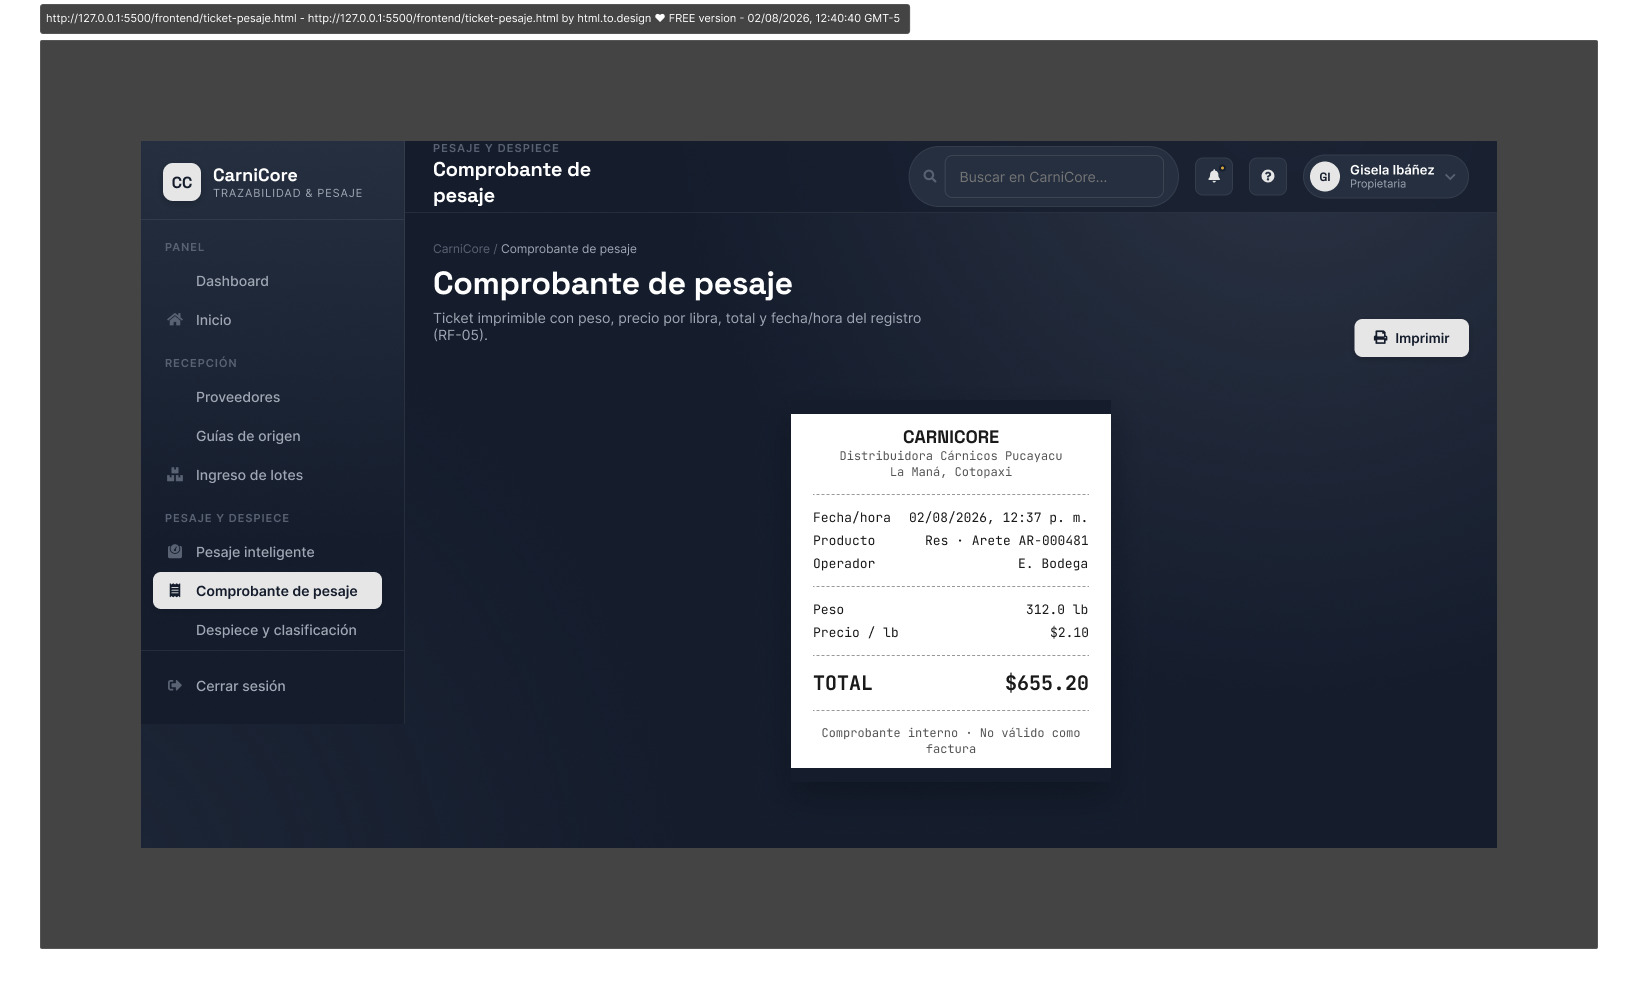
\includegraphics[width=\textwidth,keepaspectratio]{figures/MU-19_comprobante_pesaje.jpg}
    \caption{MU-19 Interfaz del módulo de comprobante de pesaje del Sistema}
    \label{fig:diagrama_clases}
\end{figure}

\begin{figure}[H]
    \centering
    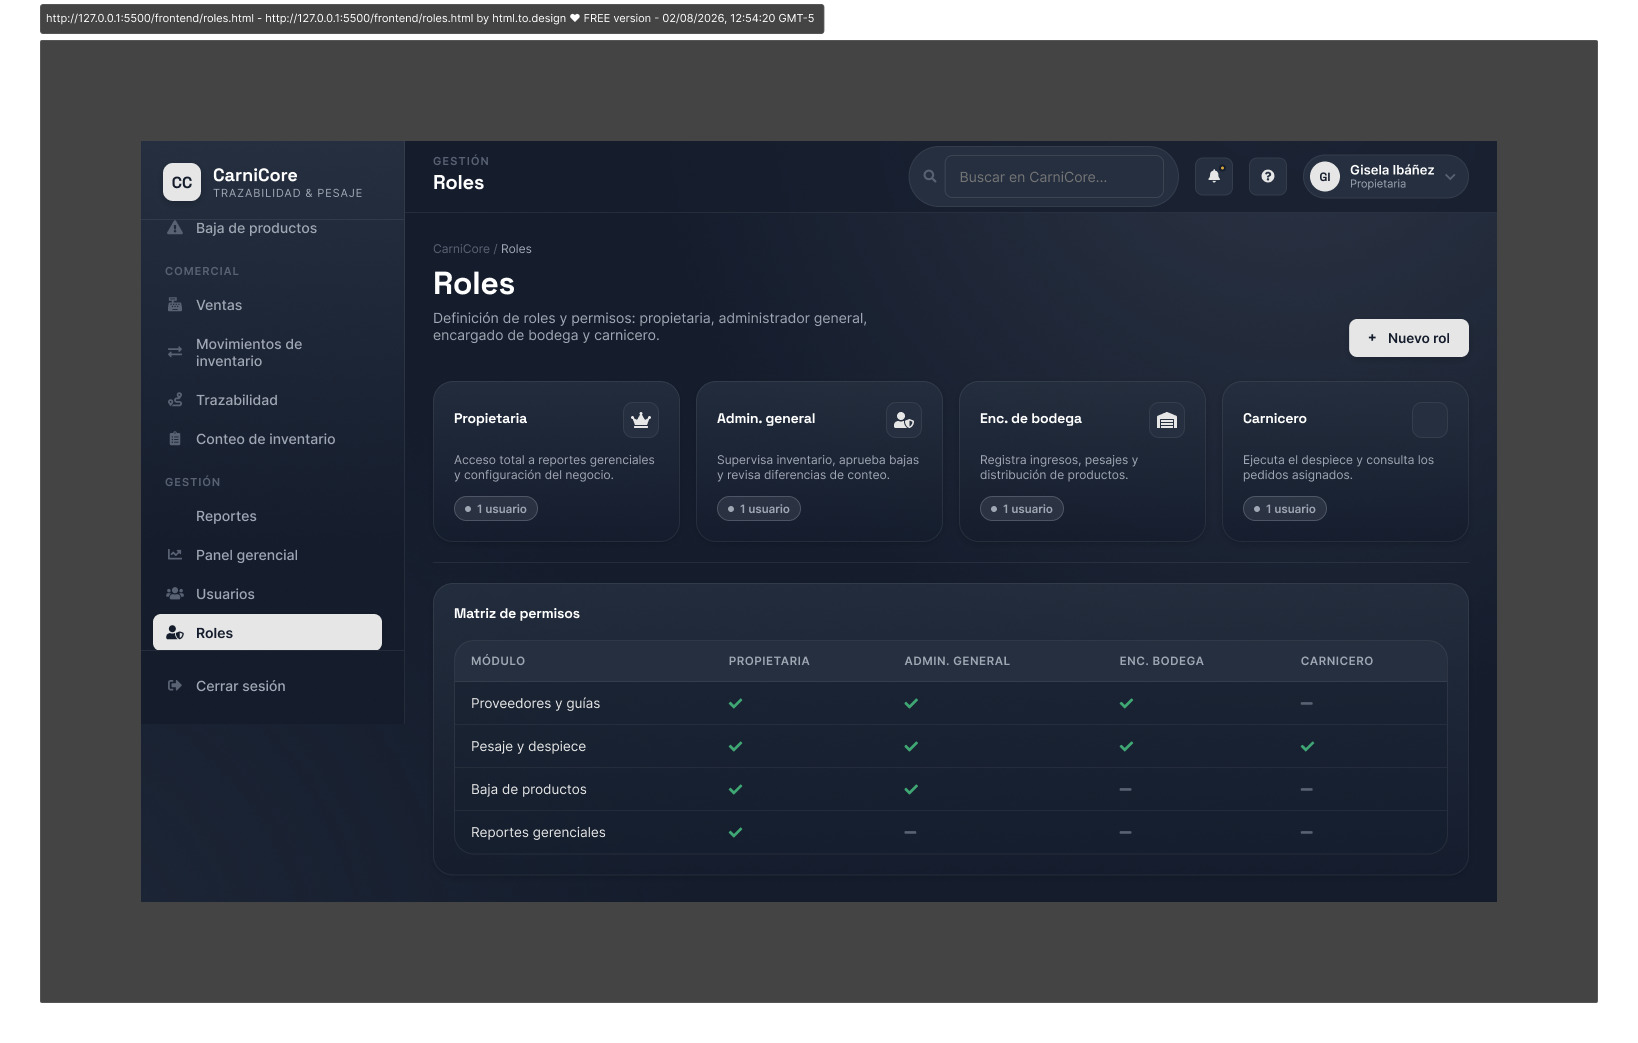
\includegraphics[width=\textwidth,keepaspectratio]{figures/MU-20_roles.jpg}
    \caption{MU-05 Interfaz del módulo de roles del Sistema}
    \label{fig:diagrama_clases}
\end{figure}


\subsubsection{Interfaces de comunicación}
Comunicación cliente-servidor mediante HTTPS; notificaciones internas (alertas de vencimiento) mediante la propia interfaz web/móvil del sistema.

\subsection{Requisitos funcionales}
Se documentan 25 requisitos funcionales con los ocho atributos exigidos por la plantilla (ID, Nombre, Descripción, Fuente, Prioridad, Estabilidad, Criterio de aceptación, Dependencias), incluyendo el Identificador de Evidencia (EV-\textit{XX}) que respalda cada uno. RF-01 a RF-16 provienen de la Entrega 1B (fuente: transcripción de la entrevista semiestructurada aplicada a la propietaria); RF-17 a RF-25 se incorporan en esta entrega a partir de la segunda ronda de elicitación.

RF-17 a RF-25 fueron confirmados con los interesados durante la segunda ronda de elicitación (entrevistas y cuestionario, semana 12), con respaldo en las evidencias EV-10 a EV-15 registradas en la matriz de trazabilidad extendida (Sección~5.2) y en las actas y consentimientos del Apéndice~B. La redacción se mantiene sin cambios respecto a la propuesta inicial del equipo, dado que los stakeholders no solicitaron ajustes durante la validación.

\newcommand{\rfitem}[8]{%
\begin{longtable}{|p{2.4cm}|p{11.2cm}|}
\hline
\multicolumn{2}{|l|}{\textbf{#1 -- #2}} \\
\hline
ID & #1 \\
\hline
Nombre & #2 \\
\hline
Descripción & #3 \\
\hline
Fuente & #4 \\
\hline
Prioridad & #5 \\
\hline
Estabilidad & #6 \\
\hline
Criterio de aceptación & #7 \\
\hline
Dependencias / EV & #8 \\
\hline
\end{longtable}
\vspace{-0.4cm}
}

\rfitem{RF-01}{Registrar proveedor}{El sistema deberá permitir registrar un proveedor de animales o derivados cárnicos, almacenando su RUC, nombre y estado de regularización ante el SRI.}{Propietaria -- Bloque 2, Pregunta 4}{Must}{Estable}{El sistema no permite registrar un proveedor sin un número de RUC válido de 13 dígitos.}{Dependencias: RF-02. EV-01.}

\rfitem{RF-02}{Registrar guía de origen}{El sistema deberá permitir registrar la guía de origen entregada por el proveedor, incluyendo número de guía, cantidad de canales y confirmación de firma del médico veterinario de planta.}{Propietaria -- Bloque 2, Pregunta 5}{Must}{Estable}{El sistema rechaza el registro de un lote si no existe una guía de origen asociada.}{Dependencias: RF-01, RF-03. EV-02.}

\rfitem{RF-03}{Registrar ingreso de lote o animal}{El sistema deberá permitir registrar el ingreso de un lote (aves) o de animales individuales (cerdo, res) identificados por número de arete, incluyendo fecha, cantidad y tipo de producto.}{Propietaria -- Bloque 3, Pregunta 10}{Must}{Estable}{Para cerdo y res, el sistema exige un número de arete único por animal; para aves, exige únicamente la cantidad ingresada.}{Dependencias: RF-02. EV-03.}

\rfitem{RF-04}{Registrar pesaje de producto}{El sistema deberá permitir registrar el peso en libras de un producto y calcular automáticamente el costo total según el precio por libra configurado.}{Propietaria -- Bloque 6, Pregunta 29}{Must}{Estable}{Al ingresar peso y precio por libra, el sistema calcula y muestra el costo total en menos de 1 segundo.}{Dependencias: RF-03. EV-04.}

\rfitem{RF-05}{Emitir comprobante de pesaje}{El sistema deberá generar un comprobante (ticket) con peso, precio por libra y costo total, imprimible o exportable en formato digital.}{Propietaria -- Bloque 6, Pregunta 29}{Should}{Estable}{El comprobante incluye peso, precio unitario, costo total y fecha/hora del registro.}{Dependencias: RF-04. EV-04.}

\rfitem{RF-06}{Registrar despiece y clasificación de cortes}{El sistema deberá permitir registrar los cortes obtenidos al despostar un animal (brazos, piernas, costillas, lomos, cabezas) y su peso individual.}{Propietaria -- Bloque 5, Preguntas 23 y 25}{Must}{Estable}{La suma de los pesos de los cortes no supera el peso del animal ingresado, con un margen de merma configurable.}{Dependencias: RF-03. EV-05.}

\rfitem{RF-07}{Registrar ingreso de producto a cámara frigorífica}{El sistema deberá permitir registrar el ingreso de un producto a una cámara frigorífica específica, indicando sección (cerdo o res) y fecha de ingreso.}{Propietaria -- Bloque 9, Pregunta 53}{Must}{Estable}{Todo producto almacenado queda asociado a una cámara y una sección válidas.}{Dependencias: RF-06. EV-06.}

\rfitem{RF-08}{Calcular y alertar vida útil del producto}{El sistema deberá calcular los días restantes de vida útil de un producto según su tipo (por ejemplo, máximo 3 días para pollo) y generar una alerta visual cuando esté próximo a vencer.}{Propietaria -- Bloque 9, Pregunta 47}{Must}{Volátil}{El sistema muestra una alerta cuando falta un día o menos para el límite de vida útil configurado por tipo de producto.}{Dependencias: RF-07. EV-06.}

\rfitem{RF-09}{Registrar baja de producto}{El sistema deberá permitir registrar la baja de un producto por vencimiento o mal estado, adjuntando peso, motivo y evidencia fotográfica, con aprobación del administrador general.}{Propietaria -- Bloque 8, Preguntas 44 y 45}{Must}{Estable}{Una baja de producto no se refleja en el inventario hasta que el administrador general la apruebe.}{Dependencias: RF-07. EV-07.}

\rfitem{RF-10}{Registrar venta o salida de producto}{El sistema deberá permitir registrar la salida de un producto por venta a un cliente o sucursal, referenciando el número de factura del sistema contable externo.}{Propietaria -- Bloque 10, Pregunta 56}{Must}{Estable}{Toda venta descuenta automáticamente el producto correspondiente del inventario de la cámara de origen.}{Dependencias: RF-07. EV-08.}

\rfitem{RF-11}{Consultar trazabilidad de producto}{El sistema deberá permitir consultar, a partir del número de arete o código de lote, la cadena completa de trazabilidad: granja de origen, guía de origen, faenamiento, pesaje, cámara y venta.}{Propietaria -- Bloque 3, Pregunta 12}{Must}{Estable}{Ante un número de arete válido, el sistema muestra la cadena de trazabilidad completa en menos de 3 segundos.}{Dependencias: RF-02, RF-03, RF-04, RF-06, RF-07, RF-10. EV-03.}

\rfitem{RF-12}{Realizar conteo de inventario}{El sistema deberá permitir registrar un conteo físico semanal de inventario por cámara y comparar el resultado contra el inventario del sistema, calculando diferencias.}{Propietaria -- Bloque 8, Pregunta 43}{Should}{Estable}{El sistema muestra automáticamente la diferencia en libras y en valor monetario entre el conteo físico y el inventario registrado.}{Dependencias: RF-07, RF-09. EV-09.}

\rfitem{RF-13}{Generar reportes de ventas, compras y pérdidas}{El sistema deberá generar reportes filtrables por rango de fechas y tipo de producto, mostrando totales de ventas, compras y pérdidas por baja de producto.}{Propietaria -- Bloque 10, Pregunta 55}{Must}{Estable}{El reporte generado puede exportarse en PDF y refleja el mismo total que la suma de los registros individuales del período consultado.}{Dependencias: RF-09, RF-10. EV-08.}

\rfitem{RF-14}{Visualizar panel resumen del negocio}{El sistema deberá presentar un panel gráfico con las ventas por tipo de producto, el cliente que más compró y el producto de mayor rotación en un período determinado.}{Propietaria -- Bloque 10, Pregunta 56}{Should}{Volátil}{El panel se actualiza automáticamente al registrarse una nueva venta, sin requerir recarga manual de la página.}{Dependencias: RF-10, RF-13. EV-08.}

\rfitem{RF-15}{Gestionar usuarios y roles}{El sistema deberá permitir crear, editar y desactivar usuarios, asignándoles uno de los roles definidos (propietaria, administrador general, encargado de bodega, carnicero).}{Propietaria -- Bloque 1, Preguntas 2 y 3}{Must}{Estable}{Un usuario desactivado no puede iniciar sesión ni realizar ninguna operación en el sistema.}{Dependencias: Ninguna. EV-01.}

\rfitem{RF-16}{Registrar movimientos de inventario por fecha}{El sistema deberá registrar cada ingreso y egreso de producto por cámara y fecha, permitiendo consultar el stock disponible en cada local en un momento determinado.}{Propietaria -- Pregunta complementaria de reporte de movimientos}{Must}{Estable}{El sistema permite consultar el stock de un producto específico a una fecha dada con un margen de error de 0\% respecto a los movimientos registrados.}{Dependencias: RF-07, RF-09, RF-10. EV-09.}

\rfitem{RF-17}{Registrar georreferencia de proveedor/granja}{El sistema deberá permitir asociar coordenadas geográficas aproximadas de la granja de origen al perfil del proveedor, para enriquecer la consulta de trazabilidad.}{Segunda ronda -- Administrador general}{Should}{Estable}{Un proveedor sin coordenadas registradas puede operar normalmente; el campo es opcional pero, si se ingresa, valida rango de latitud/longitud de Ecuador continental.}{Dependencias: RF-01. EV-17 (confirmado con evidencia real de la segunda ronda, registrada como EV-10 en la matriz de trazabilidad extendida, Sección~5.2).}

\rfitem{RF-18}{Consultar historial de precios por libra}{El sistema deberá permitir consultar el histórico de precios por libra configurados para cada tipo de producto en un rango de fechas.}{Segunda ronda -- Propietaria}{Could}{Estable}{El histórico muestra, para cada cambio de precio, la fecha, el precio anterior, el precio nuevo y el usuario que lo modificó.}{Dependencias: RF-04. EV-18 (confirmado con evidencia real de la segunda ronda, registrada como EV-11 en la matriz de trazabilidad extendida, Sección~5.2).}

\rfitem{RF-19}{Configurar precios por tipo de producto y temporada}{El sistema deberá permitir a la propietaria o al administrador general configurar el precio por libra vigente para cada tipo de producto, con posibilidad de definir una fecha de vigencia futura.}{Segunda ronda -- Propietaria}{Must}{Estable}{Un precio con fecha de vigencia futura no se aplica a los pesajes registrados antes de esa fecha.}{Dependencias: RF-04. EV-19 (confirmado con evidencia real de la segunda ronda, registrada como EV-11 en la matriz de trazabilidad extendida, Sección~5.2).}

\rfitem{RF-20}{Registrar incidentes de corte de energía}{El sistema deberá permitir registrar un incidente de corte de energía eléctrica, indicando fecha, hora de inicio, hora de restablecimiento y cámaras afectadas, como insumo para sustentar posibles bajas de producto.}{Segunda ronda -- Propietaria (hallazgo de apagones)}{Must}{Estable}{Todo incidente registrado queda disponible como evidencia asociable a una baja de producto (RF-09) generada por pérdida de cadena de frío.}{Dependencias: RF-07. EV-20 (confirmado con evidencia real de la segunda ronda, registrada como EV-12 en la matriz de trazabilidad extendida, Sección~5.2).}

\rfitem{RF-21}{Operar en modo de contingencia offline}{El sistema deberá permitir registrar operaciones críticas de bodega (ingreso, pesaje) sin conexión a internet y sincronizarlas automáticamente al restablecerse la conectividad.}{Segunda ronda -- Encargado de bodega}{Must}{Volátil}{Toda operación registrada en modo offline se sincroniza sin pérdida de datos dentro de los 5 minutos posteriores a la reconexión.}{Dependencias: RF-03, RF-04. EV-21 (confirmado con evidencia real de la segunda ronda, registrada como EV-13 en la matriz de trazabilidad extendida, Sección~5.2).}

\rfitem{RF-22}{Registrar devoluciones de clientes}{El sistema deberá permitir registrar la devolución total o parcial de un producto vendido, reingresándolo al inventario o dándolo de baja según su estado.}{Segunda ronda -- Encargado de bodega}{Should}{Estable}{Toda devolución queda vinculada a la venta original mediante el número de factura referenciado.}{Dependencias: RF-10, RF-09. EV-22 (confirmado con evidencia real de la segunda ronda, registrada como EV-14 en la matriz de trazabilidad extendida, Sección~5.2).}

\rfitem{RF-23}{Exportar evidencia de trazabilidad para auditoría}{El sistema deberá permitir exportar, en PDF o CSV, la cadena de trazabilidad completa de un lote o animal para su presentación ante auditorías de Agrocalidad.}{Segunda ronda -- Administrador general}{Must}{Estable}{El archivo exportado contiene los mismos datos mostrados en la consulta de trazabilidad (RF-11) y conserva el formato exigido por Agrocalidad.}{Dependencias: RF-11. EV-23 (confirmado con evidencia real de la segunda ronda, registrada como EV-15 en la matriz de trazabilidad extendida, Sección~5.2).}

\rfitem{RF-24}{Buscar producto por código de lote en catálogo de cámaras}{El sistema deberá permitir buscar y filtrar productos almacenados en cámaras frigoríficas por código de lote, tipo de producto o sección.}{Segunda ronda -- Encargado de bodega}{Should}{Estable}{Una búsqueda por código de lote válido retorna el producto en menos de 2 segundos.}{Dependencias: RF-07. EV-24 (confirmado con evidencia real de la segunda ronda, registrada como EV-09 en la matriz de trazabilidad extendida, Sección~5.2).}

\rfitem{RF-25}{Generar código QR de trazabilidad}{El sistema deberá generar un código QR asociado a cada lote o animal que, al ser escaneado, dirija a la consulta pública de trazabilidad (RF-11) con los datos autorizados para consulta externa.}{Segunda ronda -- Cliente / Propietaria}{Could}{Estable}{El código QR generado enlaza correctamente a la vista pública de trazabilidad del lote/animal correspondiente.}{Dependencias: RF-11. EV-25 (confirmado con evidencia real de la segunda ronda, registrada como EV-03 en la matriz de trazabilidad extendida, Sección~5.2).}

\subsection{Requisitos no funcionales}
Los 15 requisitos no funcionales se organizan según las nueve características de calidad de ISO/IEC~25010:2023 \cite{iso25010}: adecuación funcional, eficiencia de desempeño, compatibilidad, interacción de usuario, fiabilidad, seguridad, mantenibilidad, portabilidad y flexibilidad.

\begin{longtable}{|p{1.4cm}|p{3cm}|p{9.5cm}|}
\hline
\textbf{ID} & \textbf{Característica ISO 25010} & \textbf{Descripción cuantificable} \\
\hline
RNF-01 & Eficiencia de desempeño & El cálculo del costo total al registrar un pesaje deberá completarse en menos de 1 segundo bajo condiciones normales de operación. \\
\hline
RNF-02 & Fiabilidad & El sistema deberá estar disponible al menos el 98\% del tiempo mensual, considerando ventanas de mantenimiento fuera del horario de faenamiento (2:00--10:00 a.m.). \\
\hline
RNF-03 & Seguridad & El acceso al sistema deberá requerir autenticación mediante usuario y contraseña, con contraseñas almacenadas usando un algoritmo de hash con salting (por ejemplo, bcrypt). \\
\hline
RNF-04 & Interacción de usuario (Usabilidad) & Un encargado de bodega sin experiencia previa en sistemas informáticos deberá poder completar el registro de un ingreso de lote en un máximo de 5 minutos tras una capacitación de 30 minutos. \\
\hline
RNF-05 & Mantenibilidad & El sistema deberá seguir una arquitectura en capas (presentación, lógica de negocio, acceso a datos) que permita agregar un nuevo tipo de reporte sin modificar el módulo de pesaje ni el de trazabilidad. \\
\hline
RNF-06 & Portabilidad & La interfaz de usuario deberá ser accesible desde navegadores web modernos (Chrome, Edge, Firefox en sus dos últimas versiones mayores) sin instalación adicional. \\
\hline
RNF-07 & Seguridad (integridad de datos) & Todo registro de baja de producto deberá quedar auditado con usuario, fecha y hora, y no podrá eliminarse una vez aprobado por el administrador general. \\
\hline
RNF-08 & Adecuación funcional (completitud) & El conjunto de RF \textit{Debe tener} implementado en el MVP deberá cubrir al menos el 60\% de los RF \textit{Must} del ERS, verificable mediante la matriz de trazabilidad de la Sección~5.2. \\
\hline
RNF-09 & Compatibilidad & El módulo de pesaje deberá poder integrarse, mediante una interfaz de comunicación serial/USB o Bluetooth documentada, con al menos un modelo de báscula electrónica comercial sin requerir cambios en el modelo de datos. \\
\hline
RNF-10 & Flexibilidad (adaptabilidad) & El sistema deberá permitir agregar un nuevo tipo de producto (por ejemplo, un nuevo tipo de embutido) y su límite de vida útil sin requerir despliegue de una nueva versión del software, mediante configuración paramétrica. \\
\hline
RNF-11 & Eficiencia de desempeño & La generación de un reporte gerencial filtrado por un rango de hasta 90 días deberá completarse en menos de 5 segundos con un volumen de hasta 10\,000 registros. \\
\hline
RNF-12 & Seguridad (confidencialidad) & Los datos personales de proveedores, clientes y usuarios deberán almacenarse cifrados en reposo (AES-256) y transmitirse únicamente mediante HTTPS, conforme a la LOPDP \cite{lopd2021}. \\
\hline
RNF-13 & Interacción de usuario (accesibilidad) & Las pantallas críticas de bodega (ingreso, pesaje) deberán tener un contraste mínimo de 4.5:1 y controles táctiles de al menos 44$\times$44 px, considerando el uso con guantes en la planta. \\
\hline
RNF-14 & Fiabilidad (recuperabilidad) & Ante un corte de energía o pérdida de conectividad, el sistema deberá conservar sin pérdida las operaciones registradas en modo offline (RF-21) y recuperarlas al reiniciar el dispositivo. \\
\hline
RNF-15 & Mantenibilidad (capacidad de prueba) & El código fuente del MVP deberá contar con una cobertura de pruebas automatizadas de al menos el 40\% de las líneas correspondientes a los módulos de pesaje y trazabilidad. \\
\hline
\end{longtable}

\subsection{Requisito de explicabilidad (evaluación de aplicabilidad)}
La guía de la Entrega 3 (2A) exige un requisito de explicabilidad obligatorio para todo componente basado en Inteligencia Artificial (IA) o Aprendizaje Automático (AA) \cite{chazette2020explainability,chazette2021exploring,chazette2022explainable}. Tras revisar el alcance definido en la Sección~1.2, el equipo declara que \textbf{CarniCore no incorpora, en el alcance de esta entrega, ningún componente basado en IA o AA que produzca decisiones automáticas} (el cálculo de vida útil de RF-08 es una regla determinística de resta de fechas configurable, no un modelo aprendido). Por lo tanto, el requisito de explicabilidad se marca como \textbf{no aplicable en esta entrega} y se documenta como trabajo futuro:

\begin{itemize}[nosep]
\item \textbf{RNF-EXP-F1 (trabajo futuro):} si en una entrega posterior se incorpora un módulo de recomendación de precio o de predicción de demanda basado en AA, dicho componente deberá explicar su recomendación al usuario en menos de 2 segundos y con no más de 60 palabras, aplicando el marco de calidad de \cite{chazette2021exploring} y el proceso de evaluación de \cite{chazette2022explainable}.
\end{itemize}
Esta declaración satisface el gatekeeper G7 de la rúbrica al hacer explícita la ausencia de componentes de IA/AA y su tratamiento previsto si llegaran a incorporarse.

\subsection{Requisitos legales}
Trazabilidad explícita entre la Ley Orgánica de Protección de Datos Personales del Ecuador \cite{lopd2021} y los RF/RNF que la operacionalizan.

\begin{longtable}{|p{2.5cm}|p{6cm}|p{5cm}|}
\hline
\textbf{Artículo LOPDP} & \textbf{Obligación} & \textbf{RF/RNF que la satisface} \\
\hline
Art. 7 -- Principio de licitud y consentimiento & Todo tratamiento de datos personales de proveedores, clientes y usuarios requiere una base de licitud (consentimiento o ejecución contractual). & RF-01, RF-15 \\
\hline
Art. 9 -- Deber de información & Las personas titulares deben ser informadas sobre el tratamiento de sus datos al registrarse en el sistema. & RF-15 \\
\hline
Art. 30 -- Medidas de seguridad & El responsable del tratamiento debe implementar medidas técnicas y organizativas apropiadas. & RNF-03, RNF-12 \\
\hline
Art. 38 -- Conservación y eliminación & Los datos deben conservarse solo el tiempo necesario y eliminarse de forma segura cuando ya no se requieran. & RNF-07 (auditoría de bajas), RF-13 (reportes por período) \\
\hline
Art. 45--49 -- Derechos de las personas titulares (acceso, rectificación, eliminación) & El sistema debe permitir identificar, corregir o eliminar los datos personales de un titular a solicitud. & RF-15 (gestión de usuarios), RF-01 (gestión de proveedores) \\
\hline
\end{longtable}

\subsection{Historias de usuario (formato Connextra) y criterios de aceptación (Gherkin)}
Se redactan historias de usuario para cada RF de prioridad \textit{Debe tener} (Must), verificadas con los criterios INVEST (\textit{Independent, Negotiable, Valuable, Estimable, Small, Testable}) \cite{swebok2024} y con escenarios de aceptación en formato Gherkin (Dado--Cuando--Entonces).

\newcommand{\huitem}[4]{%
\noindent\textbf{#1} (trazada a #2)\\
\textit{Como} #3\\[0.15cm]
\textbf{Criterio de aceptación (Gherkin):}\\
#4
\vspace{0.3cm}
}

\huitem{HU-01}{RF-01}{administradora del negocio, quiero registrar un proveedor con su RUC validado, para asegurar que solo trabajo con proveedores regularizados ante el SRI.}{
\textit{Dado} que ingreso al módulo de proveedores,\\
\textit{Cuando} intento guardar un proveedor sin un RUC de 13 dígitos válido,\\
\textit{Entonces} el sistema rechaza el registro y muestra un mensaje de error.}

\huitem{HU-02}{RF-02}{encargado de bodega, quiero registrar la guía de origen de un lote, para cumplir con la trazabilidad exigida por Agrocalidad antes de aceptar el ingreso.}{
\textit{Dado} que un proveedor no tiene guía de origen registrada,\\
\textit{Cuando} intento registrar el ingreso de un lote asociado a ese proveedor,\\
\textit{Entonces} el sistema rechaza el registro del lote hasta que exista una guía de origen.}

\huitem{HU-03}{RF-03}{encargado de bodega, quiero registrar el ingreso de animales por número de arete, para mantener la trazabilidad individual exigida por Agrocalidad.}{
\textit{Dado} que registro el ingreso de un cerdo o res,\\
\textit{Cuando} el número de arete ingresado ya existe en el sistema,\\
\textit{Entonces} el sistema rechaza el registro y muestra un mensaje de duplicidad.}

\huitem{HU-04}{RF-04}{encargado de bodega, quiero que el sistema calcule automáticamente el costo total al pesar un producto, para evitar errores de cálculo manual.}{
\textit{Dado} que ingreso el peso en libras y el precio por libra configurado,\\
\textit{Cuando} confirmo el registro de pesaje,\\
\textit{Entonces} el sistema muestra el costo total calculado en menos de 1 segundo.}

\huitem{HU-06}{RF-06}{carnicero, quiero registrar el peso de cada corte obtenido al despostar un animal, para que el inventario refleje la clasificación real de productos.}{
\textit{Dado} que registro los cortes de un animal ya pesado,\\
\textit{Cuando} la suma de los pesos de los cortes supera el peso del animal más el margen de merma configurado,\\
\textit{Entonces} el sistema muestra una advertencia y solicita confirmación o corrección.}

\huitem{HU-07}{RF-07}{encargado de bodega, quiero registrar el ingreso de un producto a una cámara frigorífica específica, para mantener el inventario organizado por sección.}{
\textit{Dado} que un producto pasó por despiece o pesaje,\\
\textit{Cuando} lo registro como ingresado a una cámara sin indicar sección válida,\\
\textit{Entonces} el sistema no permite completar el registro.}

\huitem{HU-08}{RF-08}{administrador general, quiero recibir una alerta cuando un producto esté por vencer, para priorizar su venta o registrar su baja a tiempo.}{
\textit{Dado} que un producto está almacenado en cámara,\\
\textit{Cuando} falta un día o menos para el límite de vida útil configurado para su tipo,\\
\textit{Entonces} el sistema muestra una alerta visible en el panel del administrador general.}

\huitem{HU-09}{RF-09}{administrador general, quiero aprobar las bajas de producto antes de que afecten el inventario, para sustentar las pérdidas con evidencia fotográfica.}{
\textit{Dado} que un encargado de bodega registra una baja de producto,\\
\textit{Cuando} la baja aún no ha sido aprobada por el administrador general,\\
\textit{Entonces} el inventario del sistema no refleja la baja.}

\huitem{HU-10}{RF-10}{encargado de bodega, quiero registrar la venta de un producto referenciando el número de factura externo, para mantener consistencia entre el inventario y la facturación.}{
\textit{Dado} que un cliente compra un producto disponible en inventario,\\
\textit{Cuando} confirmo el registro de la venta,\\
\textit{Entonces} el sistema descuenta automáticamente el producto de la cámara de origen.}

\huitem{HU-11}{RF-11}{propietaria, quiero consultar la trazabilidad completa de un producto por su número de arete, para responder de inmediato ante un requerimiento de Agrocalidad.}{
\textit{Dado} que ingreso un número de arete válido,\\
\textit{Cuando} solicito la consulta de trazabilidad,\\
\textit{Entonces} el sistema muestra la cadena completa (granja, guía, pesaje, cámara, venta) en menos de 3 segundos.}

\huitem{HU-13}{RF-13}{propietaria, quiero generar reportes de ventas, compras y pérdidas por período, para tomar decisiones informadas de compra y venta.}{
\textit{Dado} que selecciono un rango de fechas y un tipo de producto,\\
\textit{Cuando} genero el reporte,\\
\textit{Entonces} el sistema lo exporta en PDF con un total igual a la suma de los registros individuales del período.}

\huitem{HU-15}{RF-15}{administrador general, quiero desactivar el usuario de un empleado que deja de trabajar en la distribuidora, para evitar accesos no autorizados.}{
\textit{Dado} que desactivo el usuario de un empleado,\\
\textit{Cuando} ese empleado intenta iniciar sesión,\\
\textit{Entonces} el sistema rechaza el acceso.}

\huitem{HU-16}{RF-16}{administrador general, quiero consultar el stock de un producto en una fecha pasada, para verificar diferencias de inventario reportadas por bodega.}{
\textit{Dado} que existen movimientos de ingreso y egreso registrados para un producto,\\
\textit{Cuando} consulto el stock a una fecha específica,\\
\textit{Entonces} el sistema muestra el stock con 0\% de margen de error respecto a los movimientos registrados hasta esa fecha.}

\huitem{HU-19}{RF-19}{propietaria, quiero configurar el precio por libra vigente de cada tipo de producto con una fecha de vigencia futura, para planificar cambios de precio por temporada.}{
\textit{Dado} que configuro un nuevo precio con vigencia a partir de una fecha futura,\\
\textit{Cuando} se registra un pesaje antes de esa fecha,\\
\textit{Entonces} el sistema aplica el precio anterior, no el nuevo.}

\huitem{HU-20}{RF-20}{administrador general, quiero registrar un corte de energía eléctrica, para sustentar con evidencia una eventual baja de producto por pérdida de cadena de frío.}{
\textit{Dado} que registro un incidente de corte de energía con hora de inicio y de restablecimiento,\\
\textit{Cuando} registro posteriormente una baja de producto en una cámara afectada,\\
\textit{Entonces} el sistema permite asociar el incidente como evidencia de la baja.}

\huitem{HU-21}{RF-21}{encargado de bodega, quiero seguir registrando ingresos y pesajes sin conexión a internet, para no detener la operación durante un corte de conectividad.}{
\textit{Dado} que el dispositivo pierde conectividad,\\
\textit{Cuando} registro un ingreso o un pesaje en modo offline,\\
\textit{Entonces} el sistema sincroniza la operación sin pérdida de datos dentro de los 5 minutos posteriores a la reconexión.}

\huitem{HU-23}{RF-23}{administrador general, quiero exportar la trazabilidad completa de un lote en PDF, para presentarla ante una auditoría de Agrocalidad.}{
\textit{Dado} que un lote tiene trazabilidad completa registrada,\\
\textit{Cuando} exporto la evidencia de trazabilidad,\\
\textit{Entonces} el sistema genera un archivo PDF con los mismos datos mostrados en la consulta de trazabilidad.}

Las 17 historias de usuario documentadas cubren la totalidad de los RF de prioridad \textit{Debe tener} (Must) del sistema (RF-01, 02, 03, 04, 06, 07, 08, 09, 10, 11, 13, 15, 16, 19, 20, 21, 23), cada una verificada informalmente contra los seis criterios INVEST (Independiente, Negociable, Valiosa, Estimable, Pequeña, Verificable) al redactar su criterio de aceptación en Gherkin. La validación formal con los stakeholders reales se realizó en la ronda de \textit{walkthrough} documentada en el Apéndice~B (\texttt{02\_Evidencias/Validacion\_Walkthrough/}).

\subsection{Restricciones de diseño}
\begin{enumerate}[nosep]
\item El módulo de trazabilidad deberá modelar de forma diferenciada el registro por animal individual (cerdo, res) y el registro por lote agregado (aves).
\item El cálculo de vida útil deberá ser configurable por tipo de producto (parametrizable), dado que los límites de conservación difieren sustancialmente entre pollo, res y cerdo.
\item El sistema deberá diseñarse considerando conectividad intermitente en la planta de La Maná, por lo que las operaciones críticas de bodega deberán poder registrarse en modo de contingencia y sincronizarse posteriormente (RF-21, RNF-14).
\item El diseño de la base de datos deberá separar claramente el modelo del dominio cárnico (animal, lote, corte) del modelo de facturación, gestionado por el sistema contable externo.
\item La configuración de precios (RF-19) y de límites de vida útil (RD-2) deberá almacenarse en tablas paramétricas editables por la propietaria o el administrador general, sin requerir intervención del equipo de desarrollo.
\end{enumerate}

%======================================================
\section{Modelado del Sistema con UML}
%======================================================
\subsection{Diagrama general de casos de uso}
\begin{figure}[H]
    \centering
    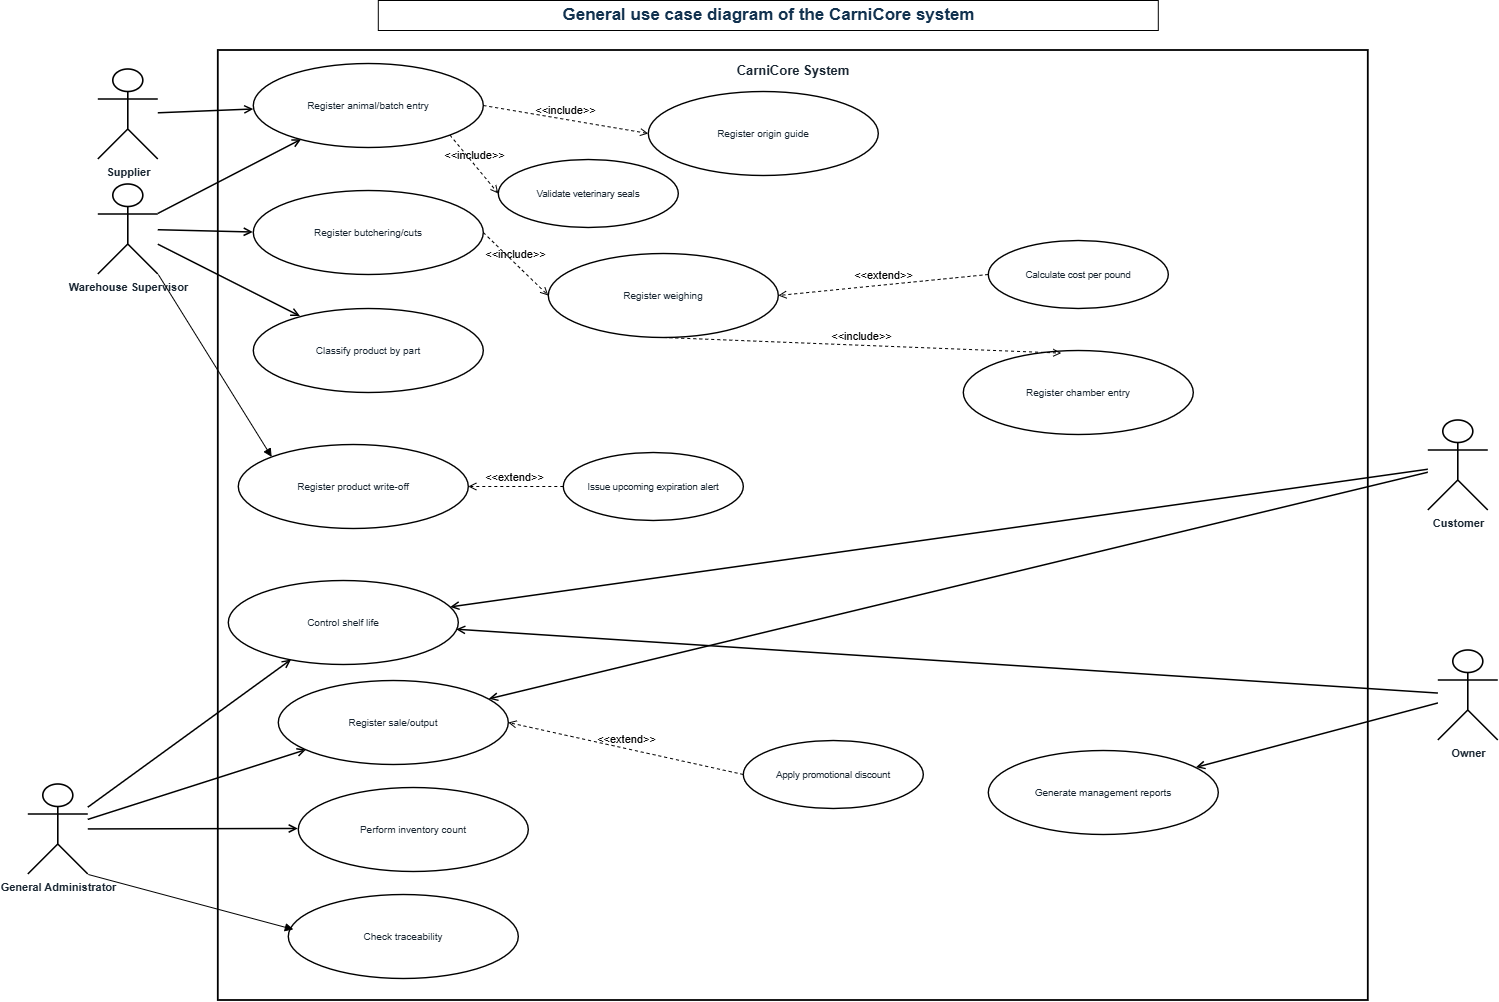
\includegraphics[width=\textwidth,keepaspectratio]{figures/Use_case_Diagram.png}
    \caption{Diagrama de casos de uso general del sistema}
    \label{fig:diagrama_clases}
\end{figure}

\subsection{Especificación textual de casos de uso (mínimo 10 detallados)}
Se detallan los 12 casos de uso asociados a RF \textit{Debe tener}, superando el mínimo de 10 CU exigido.

\newcommand{\cuitem}[6]{%
\noindent\textbf{#1 -- #2}\\
\textbf{Actor principal:} #3\\
\textbf{Precondiciones:} #4\\
\textbf{Flujo principal:} #5\\
\textbf{Postcondiciones:} #6
\vspace{0.35cm}
}

\cuitem{CU-01}{Registrar ingreso de animal/lote}{Encargado de bodega}{Existe una guía de origen registrada (RF-02) para el proveedor correspondiente.}{
(1) El encargado selecciona ``Registrar ingreso''. (2) El sistema solicita proveedor, guía de origen y tipo de producto. (3) Para cerdo/res solicita arete por animal; para aves, la cantidad total. (4) El encargado confirma. (5) El sistema registra el lote/animal como disponible para pesaje. \textit{Excepción:} arete duplicado $\Rightarrow$ mensaje de duplicidad.}{
El lote/animal queda disponible para el pesaje (CU-03).}

\cuitem{CU-02}{Registrar guía de origen}{Encargado de bodega}{El proveedor está registrado (RF-01).}{
(1) El encargado ingresa número de guía, cantidad de canales y confirma la firma del médico veterinario. (2) El sistema invoca ``Validar sellos veterinarios'' (\textit{include}). (3) El sistema almacena la guía asociada al proveedor.}{
La guía queda disponible para asociarse a un ingreso de lote/animal (CU-01).}

\cuitem{CU-03}{Registrar pesaje}{Encargado de bodega}{El lote/animal fue registrado previamente (CU-01).}{
(1) El encargado selecciona el lote/animal. (2) El sistema solicita el peso en libras. (3) El sistema invoca ``Calcular costo por libra'' (\textit{include}) y calcula el costo total. (4) El encargado confirma. (5) El sistema emite el comprobante (RF-05). \textit{Excepción:} peso $\leq 0$ $\Rightarrow$ rechazo.}{
El producto queda disponible para despiece (CU-04) o almacenamiento directo.}

\cuitem{CU-04}{Registrar despiece/cortes}{Carnicero}{El animal fue pesado (CU-03).}{
(1) El carnicero registra cada corte obtenido (tipo, peso). (2) El sistema valida que la suma de pesos no exceda el peso del animal más el margen de merma. (3) El sistema almacena los cortes.}{
Los cortes quedan disponibles para clasificación (CU-05).}

\cuitem{CU-05}{Clasificar producto por parte}{Carnicero}{Existen cortes registrados (CU-04).}{
(1) El carnicero asigna una categoría de venta a cada corte (por ejemplo, ``para asado'', ``para molida''). (2) El sistema asocia la categoría al corte para su posterior venta.}{
El producto clasificado queda disponible para ingreso a cámara (CU-06).}

\cuitem{CU-06}{Registrar ingreso a cámara}{Encargado de bodega}{Existe producto clasificado o pesado disponible.}{
(1) El encargado selecciona el producto y la cámara/sección destino. (2) El sistema registra el ingreso con fecha y calcula la vida útil inicial. (3) El sistema actualiza el inventario de la cámara.}{
El producto queda disponible para control de vida útil (CU-07), venta (CU-09) o conteo (CU-11).}

\cuitem{CU-07}{Controlar vida útil (frescura)}{Administrador general (con notificación automática del sistema)}{El producto está almacenado en cámara (CU-06).}{
(1) El sistema calcula diariamente los días transcurridos desde el ingreso a cámara. (2) Si falta un día o menos para el límite configurado, genera una alerta en el panel del administrador. (3) El administrador prioriza la venta o registra la baja (CU-10). \textit{Excepción:} producto sin tipo configurado $\Rightarrow$ no se genera alerta, se registra para revisión manual.}{
El estado del producto se actualiza a ``próximo a vencer'' o ``vencido''.}

\cuitem{CU-08}{Consultar trazabilidad de producto}{Propietaria / Cliente}{El producto cuenta con número de arete o código de lote válido.}{
(1) El usuario ingresa el número de arete o código de lote. (2) El sistema recupera la cadena de trazabilidad completa. (3) El sistema la presenta en una línea de tiempo. \textit{Flujo alternativo:} si el usuario es un cliente externo, se muestra únicamente la información autorizada para consulta pública (sin costos internos).}{
Ninguna (operación de solo lectura).}

\cuitem{CU-09}{Registrar salida/venta de producto}{Cliente / Sucursal (registrado por el encargado de bodega)}{El producto está disponible en inventario (CU-06).}{
(1) El encargado selecciona producto y cantidad. (2) El sistema valida disponibilidad. (3) El sistema solicita el número de factura externo. (4) El sistema descuenta el producto del inventario de la cámara correspondiente. \textit{Excepción:} inventario insuficiente $\Rightarrow$ rechazo del registro.}{
El inventario y los reportes de ventas (RF-13) se actualizan automáticamente.}

\cuitem{CU-10}{Registrar baja de producto}{Encargado de bodega (solicita) / Administrador general (aprueba)}{El producto está almacenado en cámara y, opcionalmente, existe un incidente de corte de energía asociado (RF-20).}{
(1) El encargado registra peso, motivo y evidencia fotográfica. (2) El sistema envía la solicitud al administrador general. (3) El administrador aprueba o rechaza. \textit{Excepción:} sin aprobación, la baja no afecta el inventario.}{
El inventario se actualiza solo tras la aprobación; el registro queda auditado (RNF-07).}

\cuitem{CU-11}{Realizar conteo de inventario}{Administrador general}{Existe inventario registrado por cámara (CU-06).}{
(1) El administrador registra el conteo físico semanal por cámara. (2) El sistema compara el conteo contra el inventario registrado. (3) El sistema calcula y muestra la diferencia en libras y en valor monetario.}{
Las diferencias quedan documentadas para su revisión gerencial.}

\cuitem{CU-12}{Generar reportes gerenciales}{Propietaria}{Existen ventas, compras y bajas registradas en el período consultado.}{
(1) La propietaria selecciona rango de fechas y tipo de producto. (2) El sistema calcula totales de ventas, compras y pérdidas. (3) El sistema exporta el reporte en PDF.}{
Ninguna (operación de solo lectura); el reporte queda disponible para descarga.}

\subsection{Diagrama de clases refinado}
El modelo conceptual de la Entrega 1B (Proveedor, GuiaOrigen, Lote, Animal, RegistroPesaje, Corte, CamaraFrigorifica, ProductoAlmacenado, Venta, BajaProducto, Usuario) se refina en esta entrega incorporando las clases \texttt{IncidenteEnergia} (asociada a \texttt{CamaraFrigorifica} y a \texttt{BajaProducto}, RF-20), \texttt{ConfiguracionPrecio} (asociada a \texttt{RegistroPesaje}, RF-19) y \texttt{Devolucion} (asociada a \texttt{Venta}, RF-22), además de las operaciones principales de cada clase (por ejemplo, \texttt{RegistroPesaje.calcularCostoTotal()}, \texttt{ProductoAlmacenado.calcularDiasVidaUtil()}, \texttt{BajaProducto.aprobar()}).

\begin{figure}[H]
    \centering
    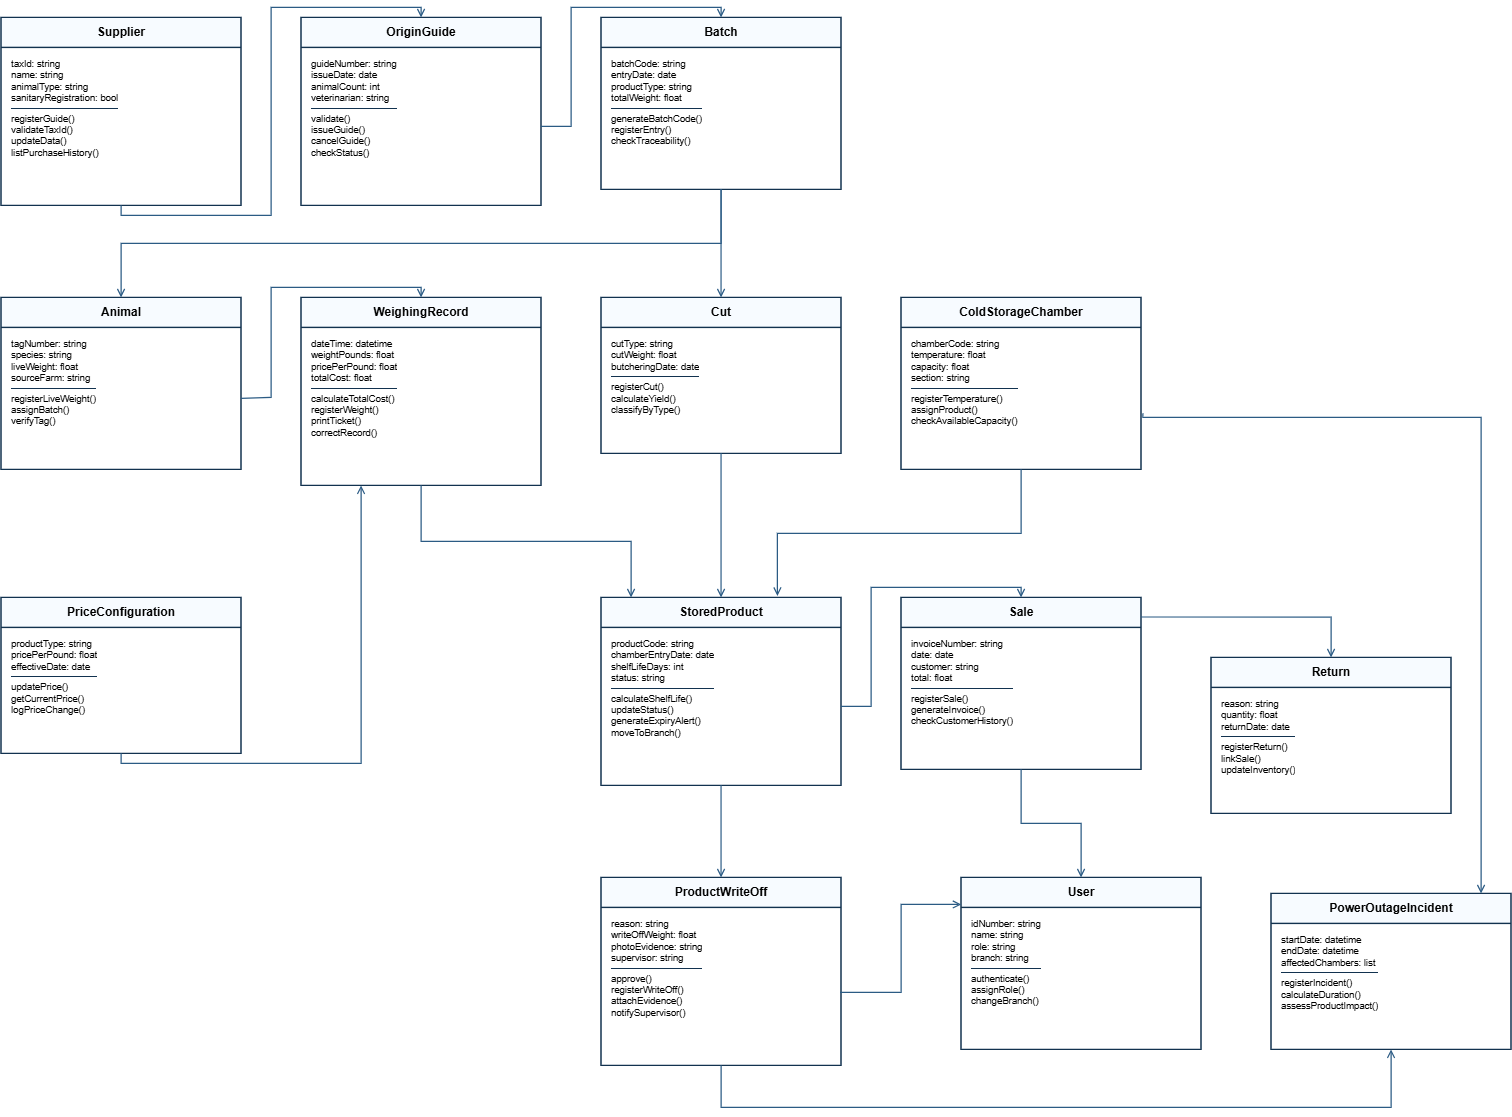
\includegraphics[width=\textwidth,keepaspectratio]{figures/Class-Diagram.png}
    \caption{Diagrama de clases del Sistema}
    \label{fig:diagrama_clases}
\end{figure}

\subsection{Diagramas de secuencia (CU-01 hasta CU-12)}
\begin{figure}[H]
    \centering
    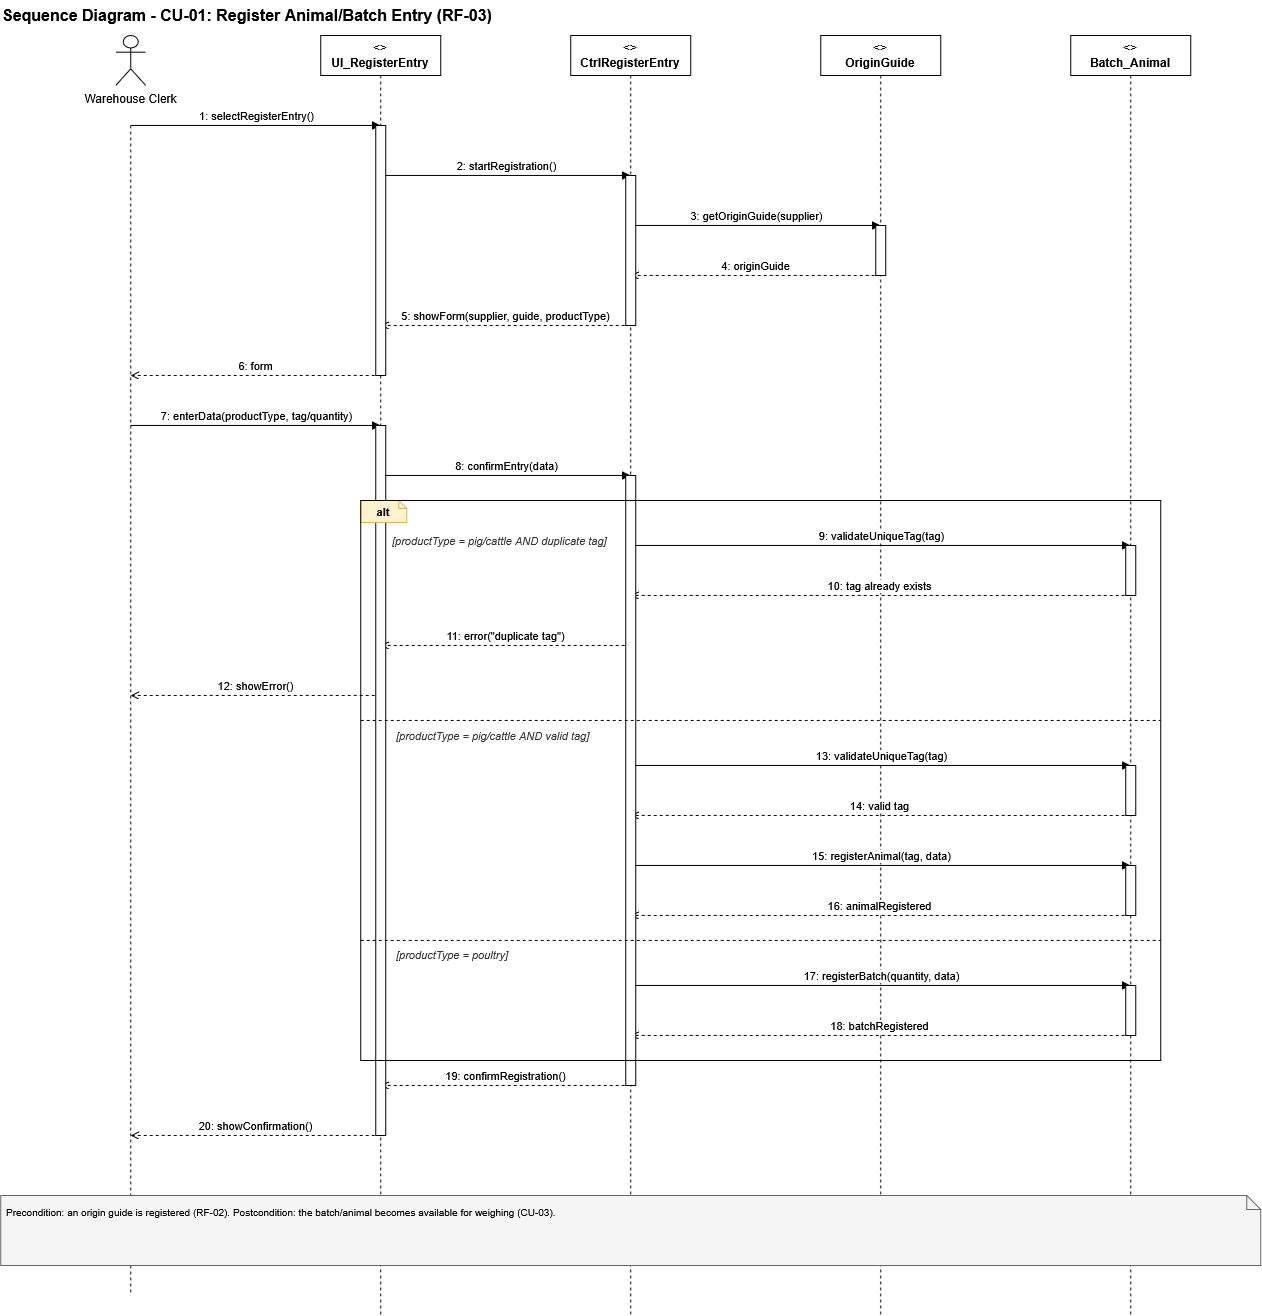
\includegraphics[width=\textwidth,keepaspectratio]{figures/01_Sequence_Diagram.png}
    \caption{Diagrama de secuencia del CU-01}
    \label{fig:diagrama_clases}
\end{figure}

\begin{figure}[H]
    \centering
    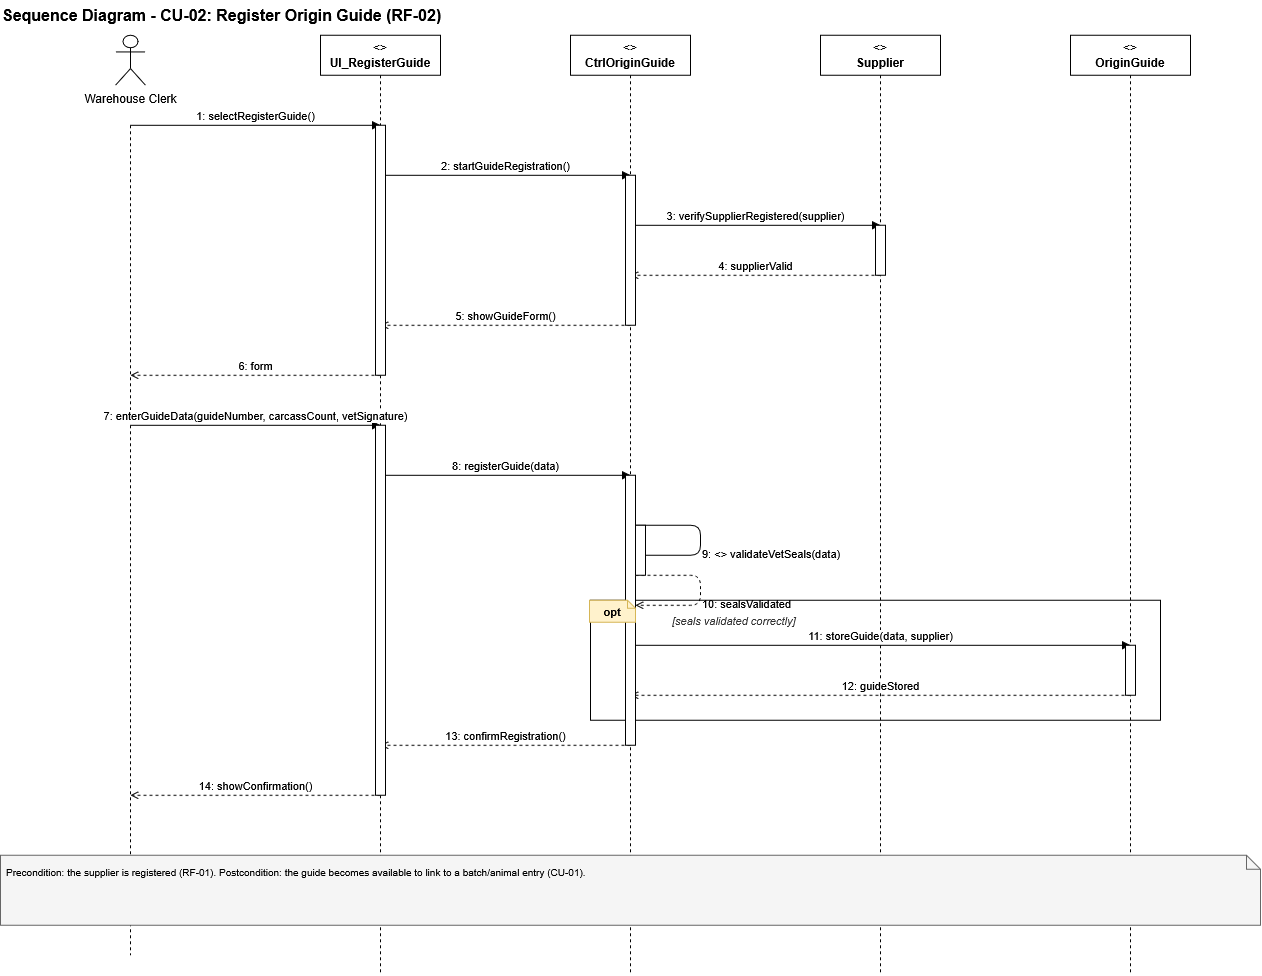
\includegraphics[width=\textwidth,keepaspectratio]{figures/02_Sequence_Diagram.png}
    \caption{Diagrama de secuencia del CU-02}
    \label{fig:diagrama_clases}
\end{figure}

\begin{figure}[H]
    \centering
    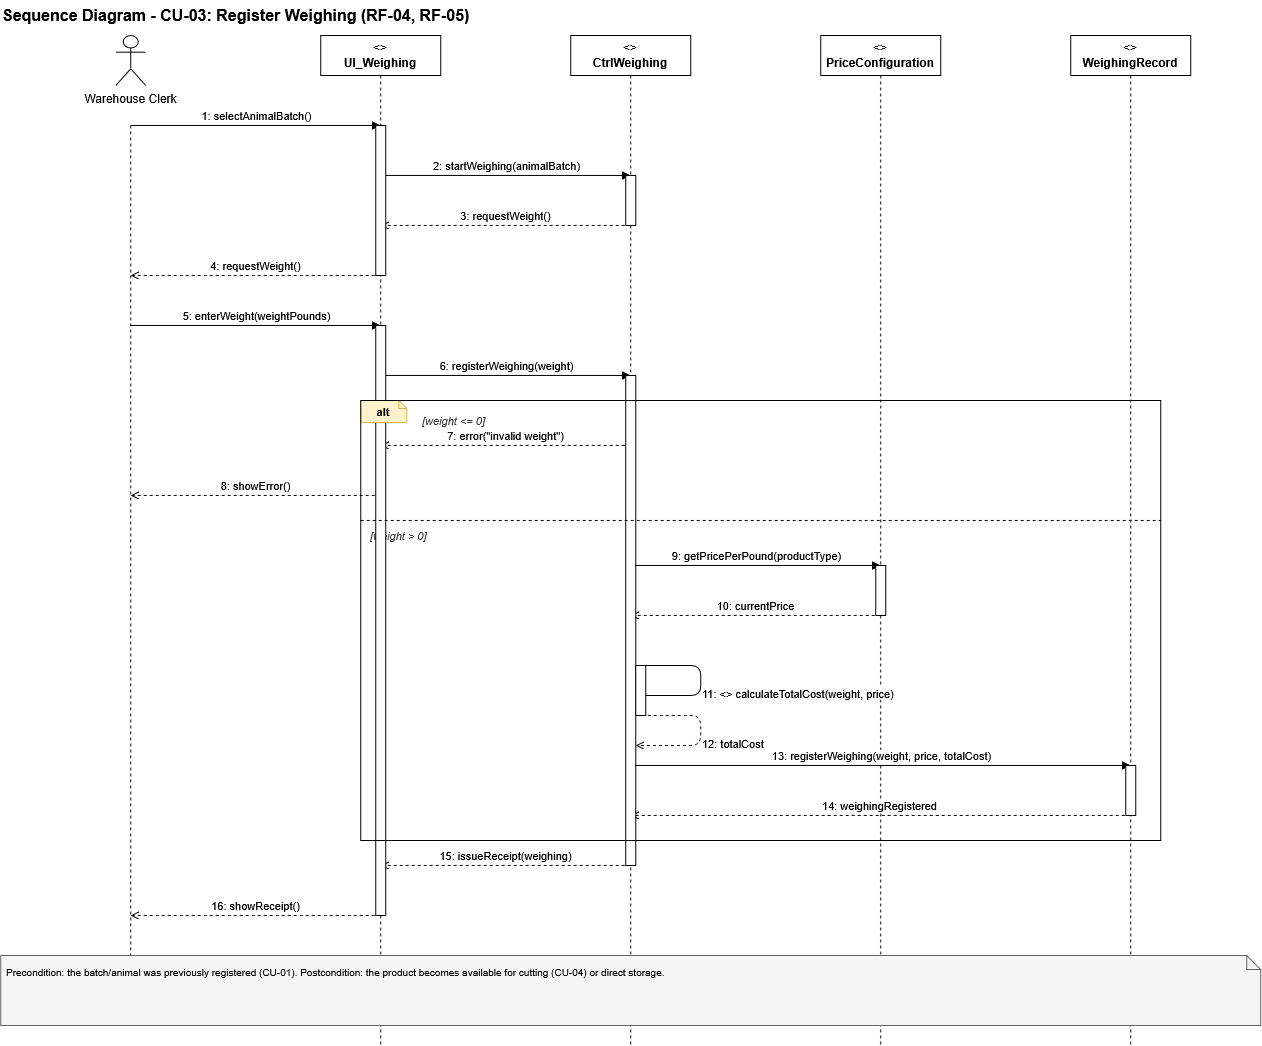
\includegraphics[width=\textwidth,keepaspectratio]{figures/03_Sequence_Diagram.png}
    \caption{Diagrama de secuencia del CU-03}
    \label{fig:diagrama_clases}
\end{figure}

\begin{figure}[H]
    \centering
    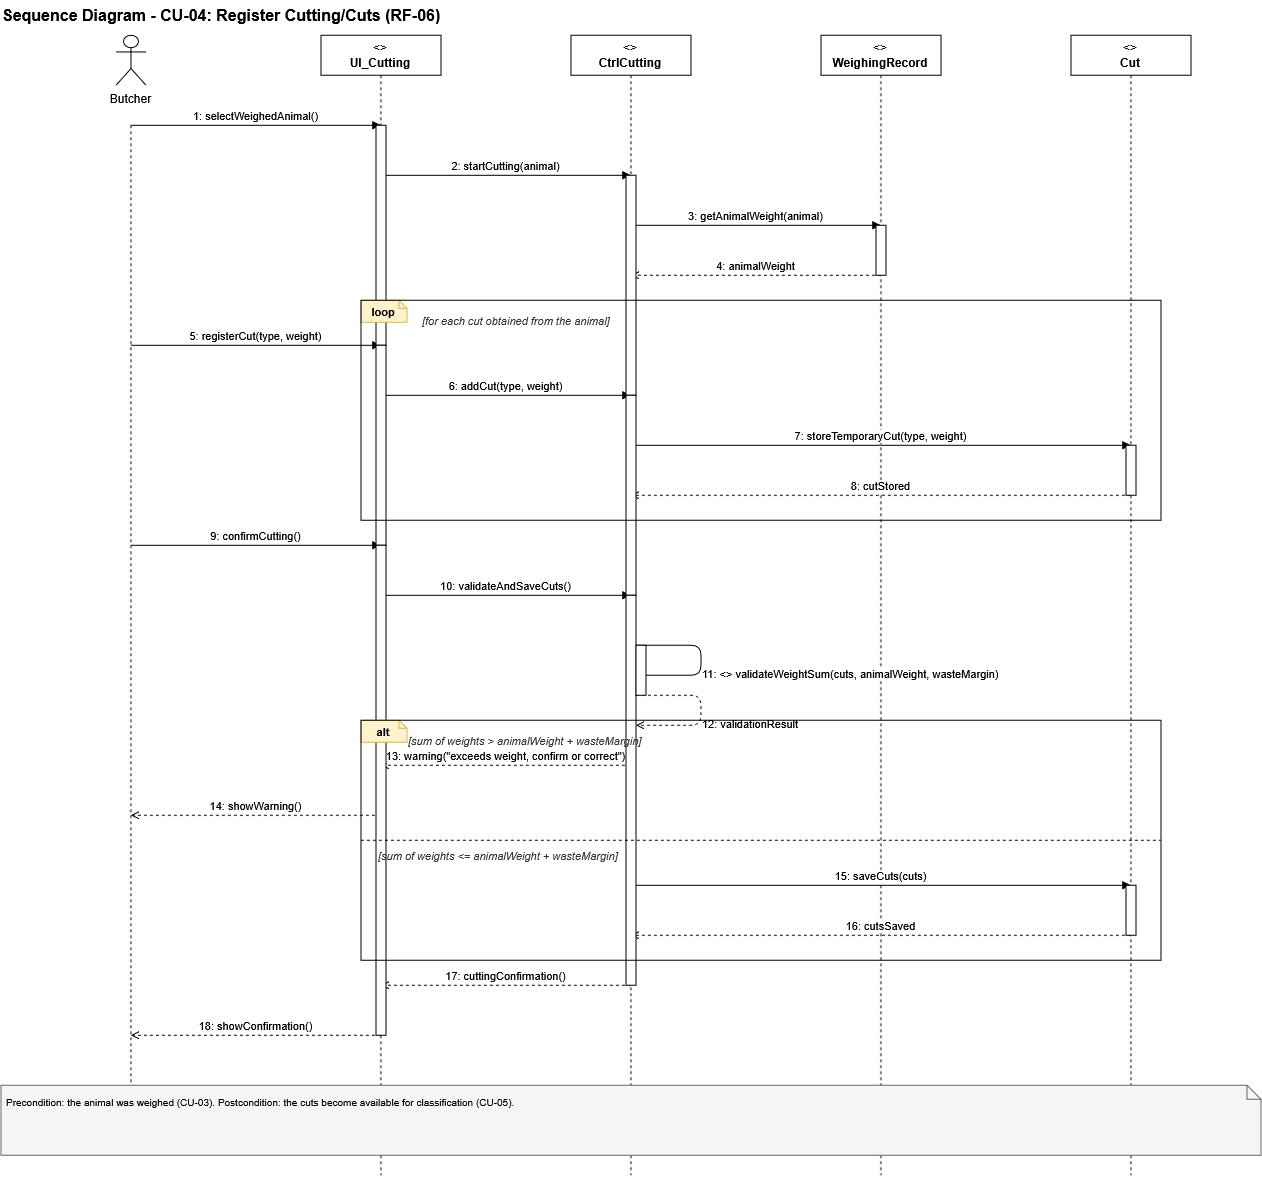
\includegraphics[width=\textwidth,keepaspectratio]{figures/04_Sequence_Diagram.png}
    \caption{Diagrama de secuencia del CU-04}
    \label{fig:diagrama_clases}
\end{figure}

\begin{figure}[H]
    \centering
    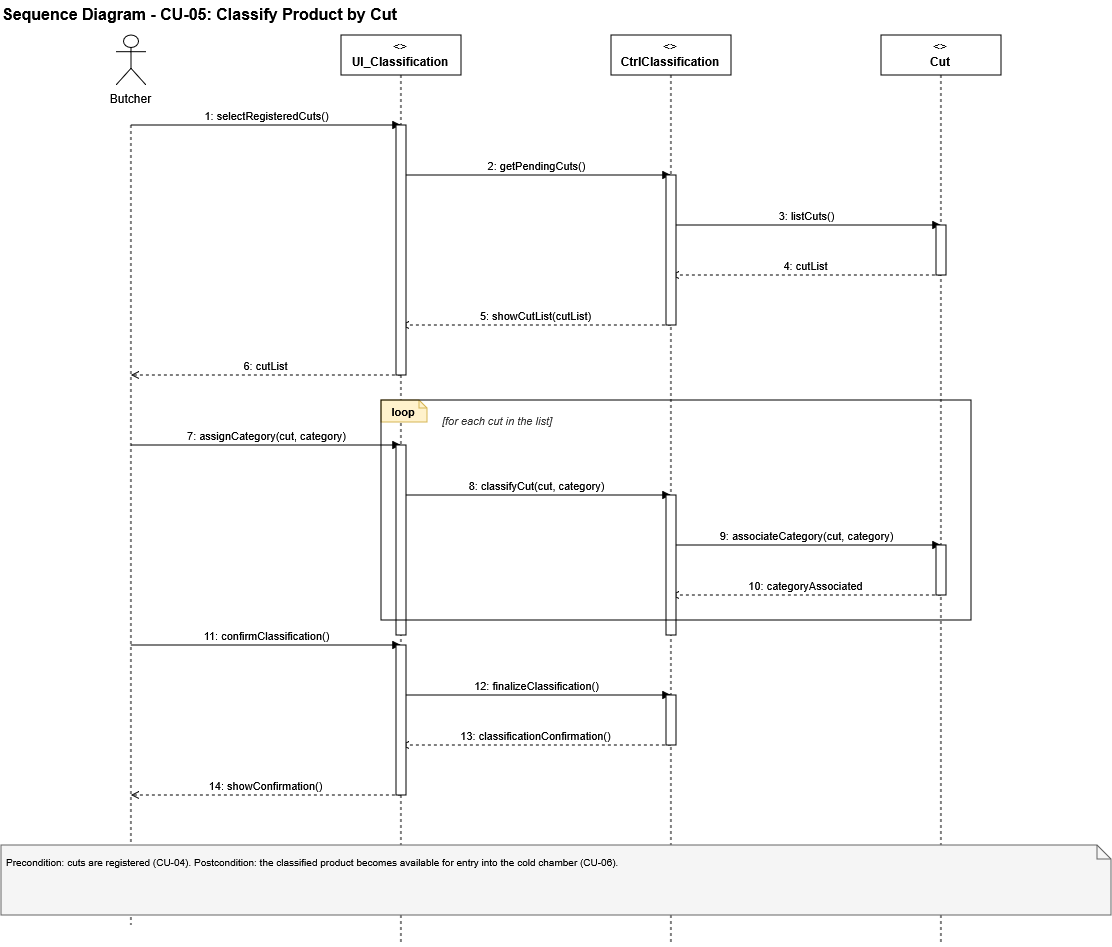
\includegraphics[width=\textwidth,keepaspectratio]{figures/05_Sequence_Diagram.png}
    \caption{Diagrama de secuencia del CU-05}
    \label{fig:diagrama_clases}
\end{figure}

\begin{figure}[H]
    \centering
    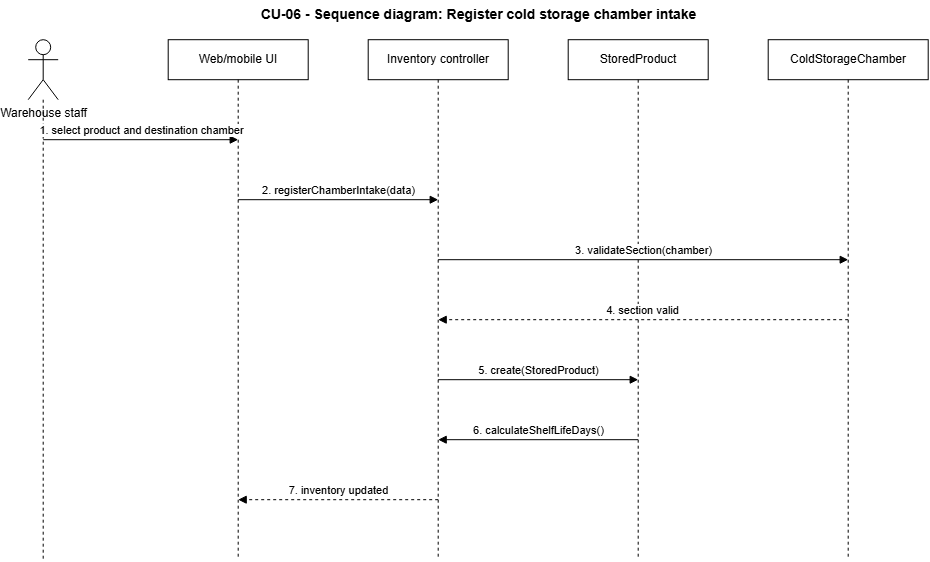
\includegraphics[width=\textwidth,keepaspectratio]{figures/06_Sequence_Diagram.png}
    \caption{Diagrama de secuencia del CU-06}
    \label{fig:diagrama_clases}
\end{figure}

\begin{figure}[H]
    \centering
    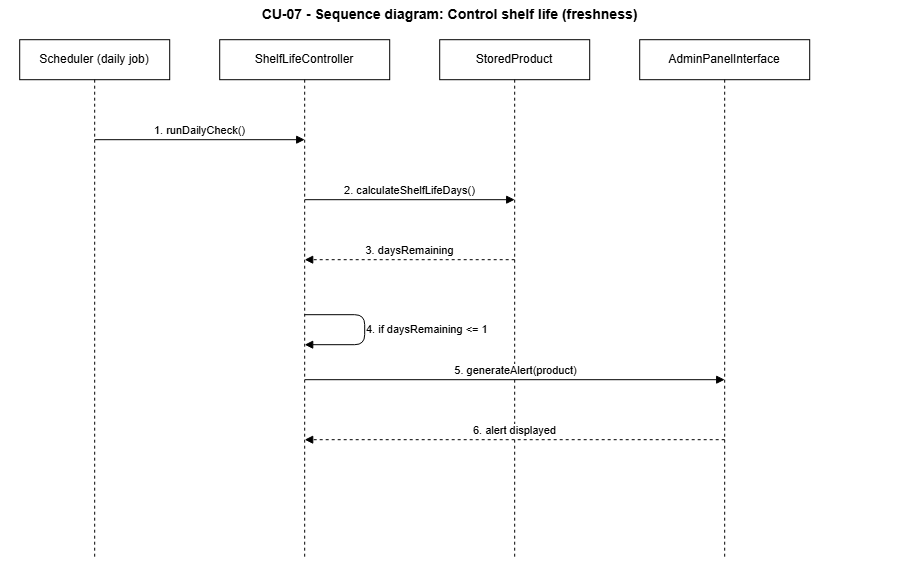
\includegraphics[width=\textwidth,keepaspectratio]{figures/07_Sequence_Diagram.png}
    \caption{Diagrama de secuencia del CU-07}
    \label{fig:diagrama_clases}
\end{figure}

\begin{figure}[H]
    \centering
    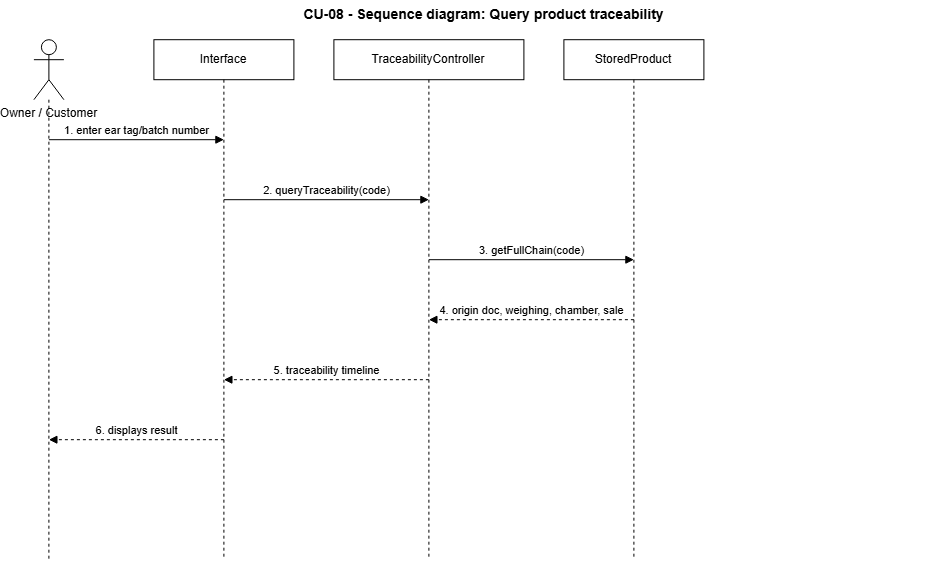
\includegraphics[width=\textwidth,keepaspectratio]{figures/08_Sequence_Diagram.png}
    \caption{Diagrama de secuencia del CU-08}
    \label{fig:diagrama_clases}
\end{figure}

\begin{figure}[H]
    \centering
    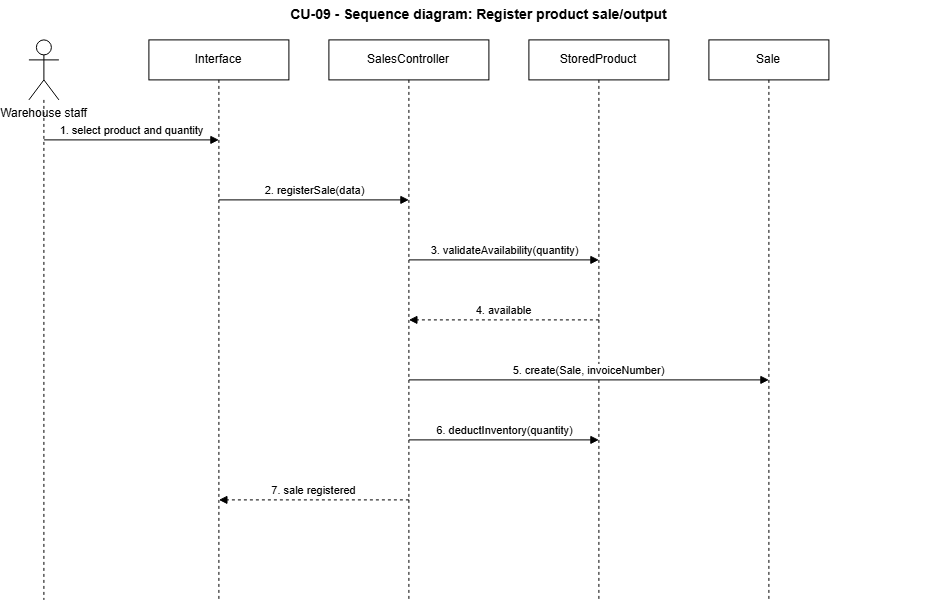
\includegraphics[width=\textwidth,keepaspectratio]{figures/09_Sequence_Diagram.png}
    \caption{Diagrama de secuencia del CU-09}
    \label{fig:diagrama_clases}
\end{figure}

\begin{figure}[H]
    \centering
    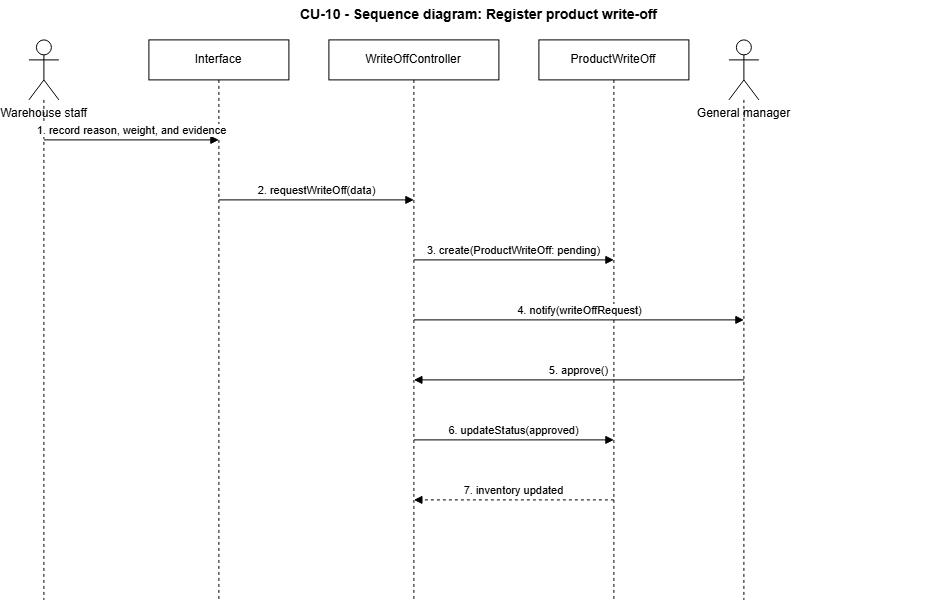
\includegraphics[width=\textwidth,keepaspectratio]{figures/10_Sequence_Diagram.png}
    \caption{Diagrama de secuencia del CU-10}
    \label{fig:diagrama_clases}
\end{figure}

\begin{figure}[H]
    \centering
    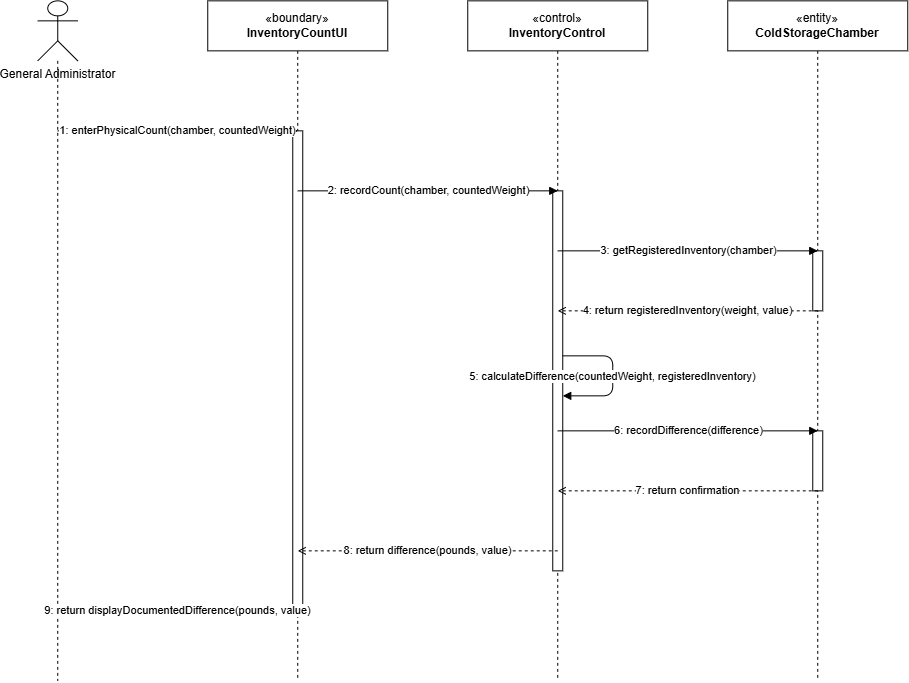
\includegraphics[width=\textwidth,keepaspectratio]{figures/11_Sequence_Diagram.png}
    \caption{Diagrama de secuencia del CU-11}
    \label{fig:diagrama_clases}
\end{figure}

\begin{figure}[H]
    \centering
    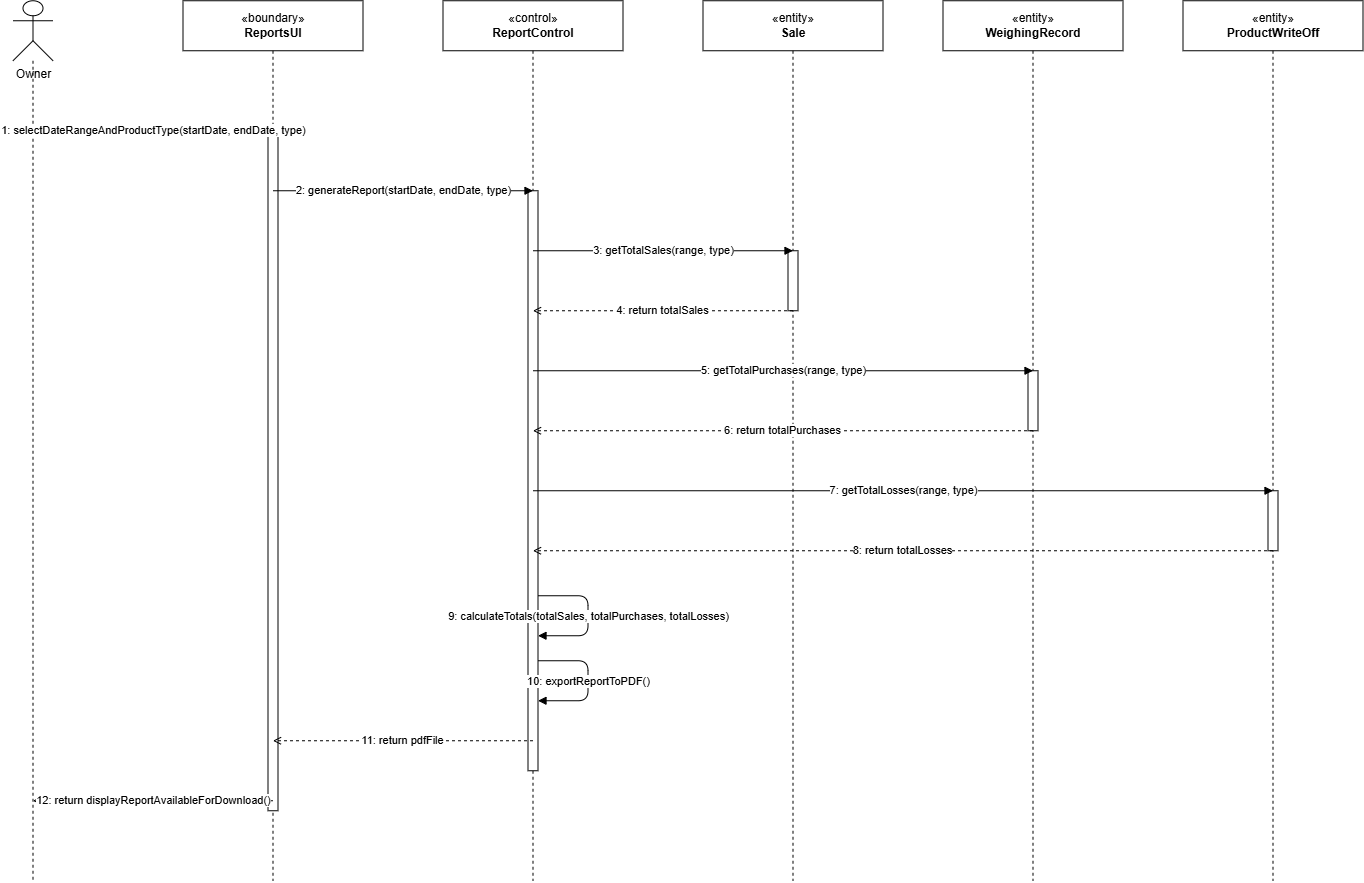
\includegraphics[width=\textwidth,keepaspectratio]{figures/12_Sequence_Diagram.png}
    \caption{Diagrama de secuencia del CU-12}
    \label{fig:diagrama_clases}
\end{figure}


\subsection{Diagramas de actividad (flujos principales)}
\begin{figure}[H]
    \centering
    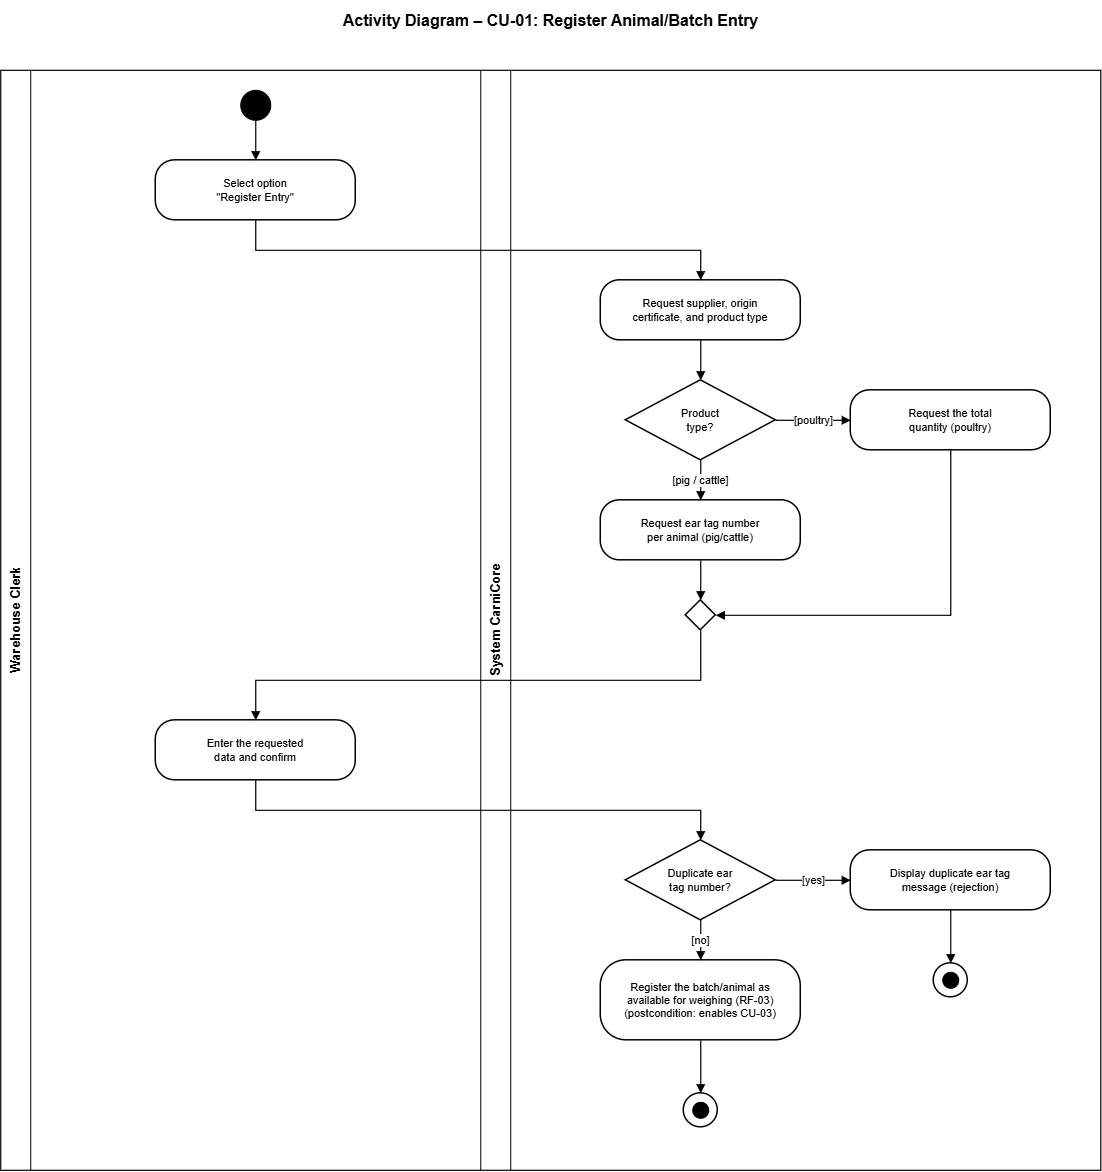
\includegraphics[width=\textwidth,keepaspectratio]{figures/01_Activity_Diagram_CU-01.png}
    \caption{Diagrama de actividad del CU-01}
    \label{fig:diagrama_clases}
\end{figure}

\subsection{Diagramas de actividad (flujos principales)}
\begin{figure}[H]
    \centering
    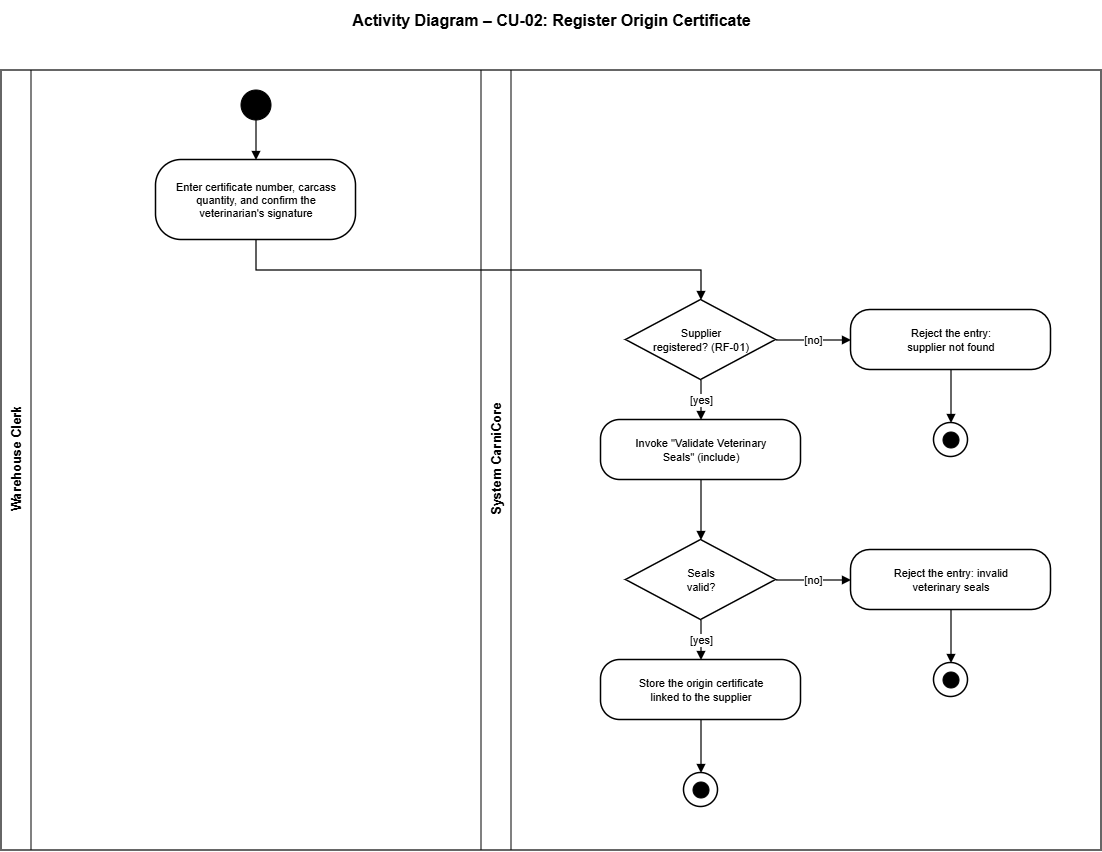
\includegraphics[width=\textwidth,keepaspectratio]{figures/02_Activity_Diagram_CU-02.png}
    \caption{Diagrama de actividad del CU-02}
    \label{fig:diagrama_clases}
\end{figure}

\subsection{Diagramas de actividad (flujos principales)}
\begin{figure}[H]
    \centering
    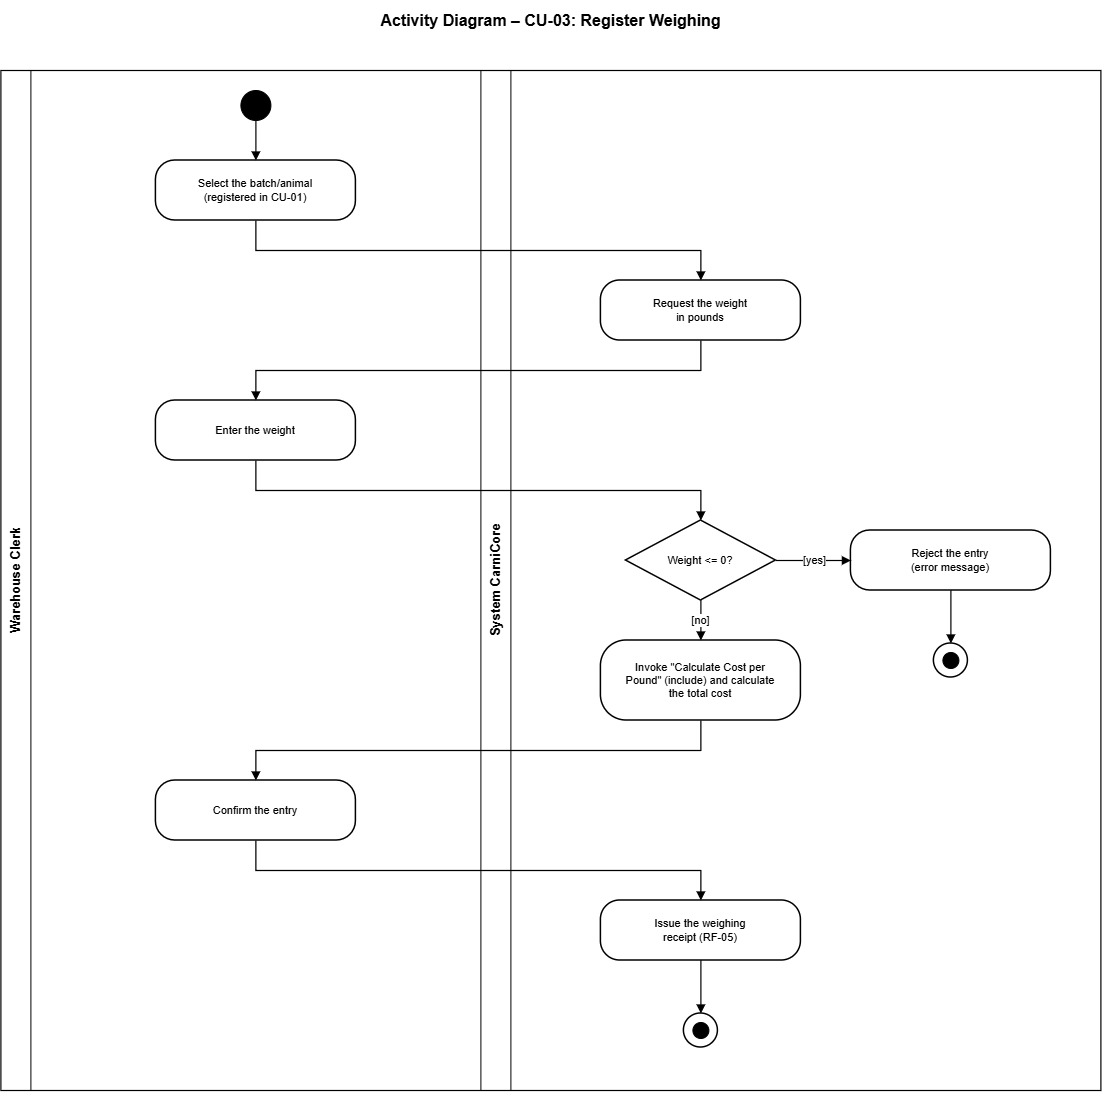
\includegraphics[width=\textwidth,keepaspectratio]{figures/03_Activity_Diagram_CU-03.png}
    \caption{Diagrama de actividad del CU-03}
    \label{fig:diagrama_clases}
\end{figure}

\subsection{Diagramas de actividad (flujos principales)}
\begin{figure}[H]
    \centering
    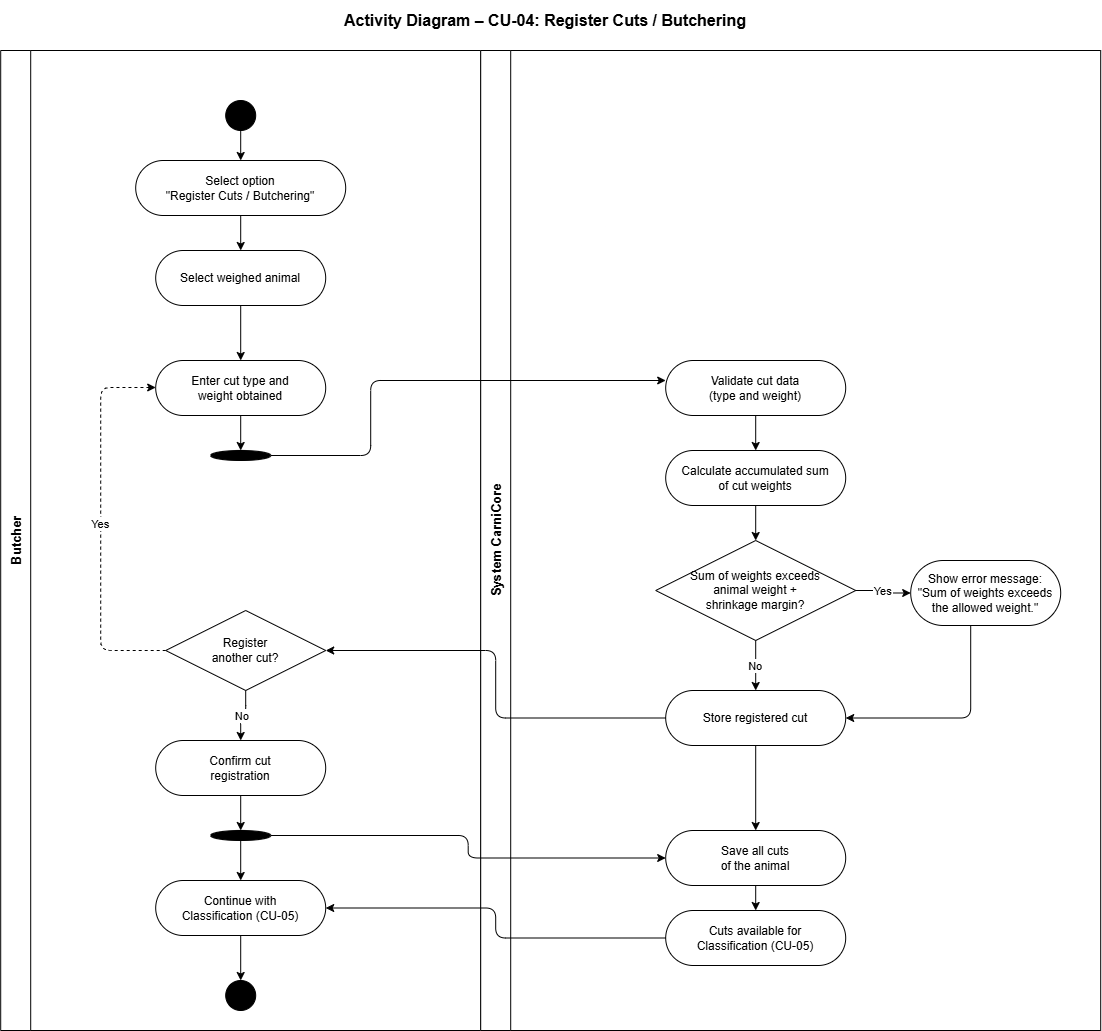
\includegraphics[width=\textwidth,keepaspectratio]{figures/04_Activity_Diagram_CU-04.png}
    \caption{Diagrama de actividad del CU-04}
    \label{fig:diagrama_clases}
\end{figure}

\subsection{Diagramas de actividad (flujos principales)}
\begin{figure}[H]
    \centering
    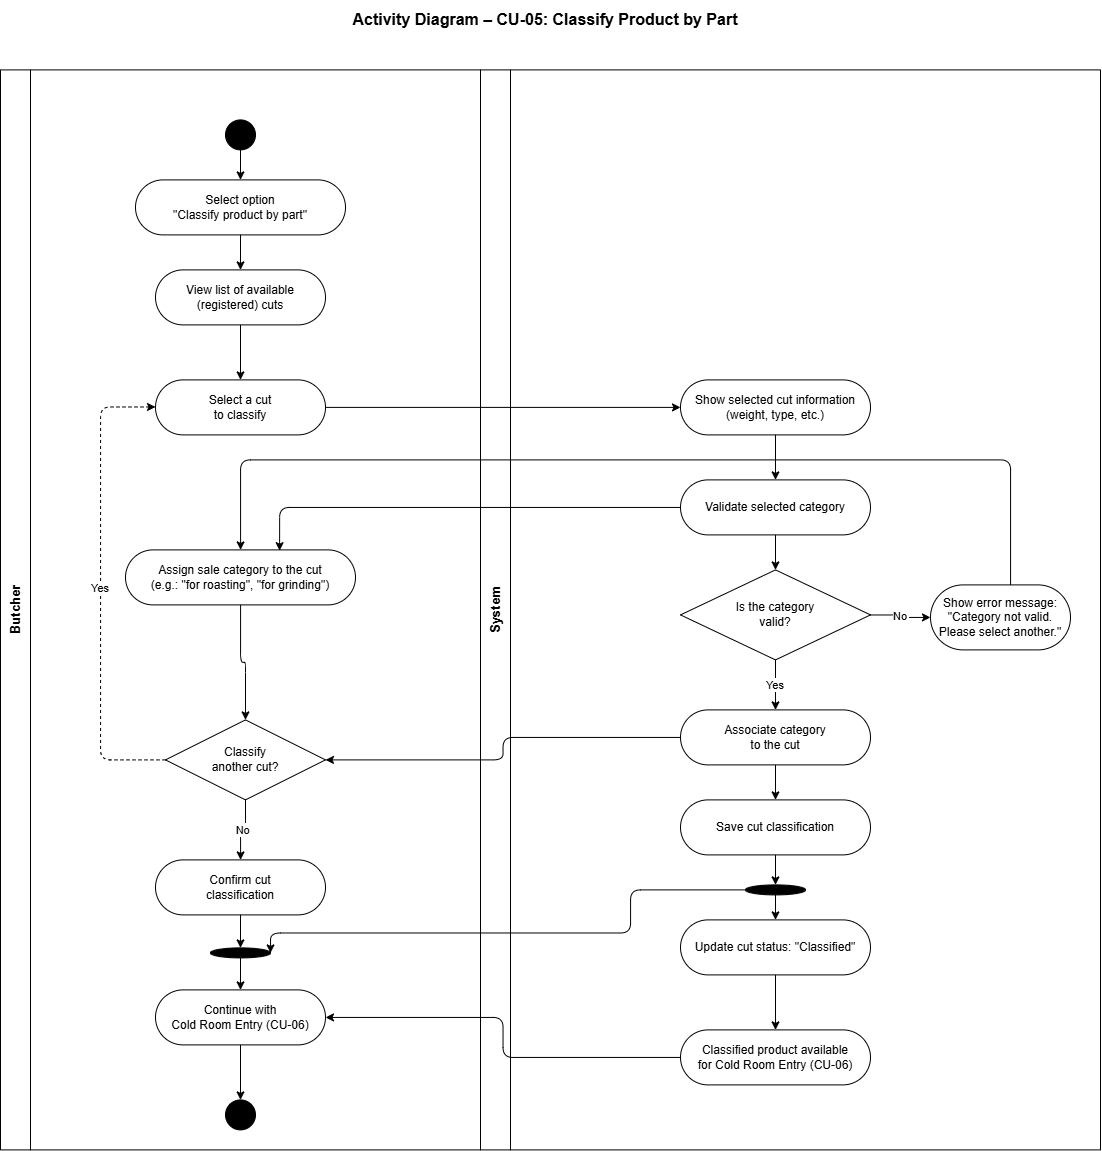
\includegraphics[width=\textwidth,keepaspectratio]{figures/05_Activity_Diagram_CU-05.png}
    \caption{Diagrama de actividad del CU-05}
    \label{fig:diagrama_clases}
\end{figure}

\subsection{Diagramas de actividad (flujos principales)}
\begin{figure}[H]
    \centering
    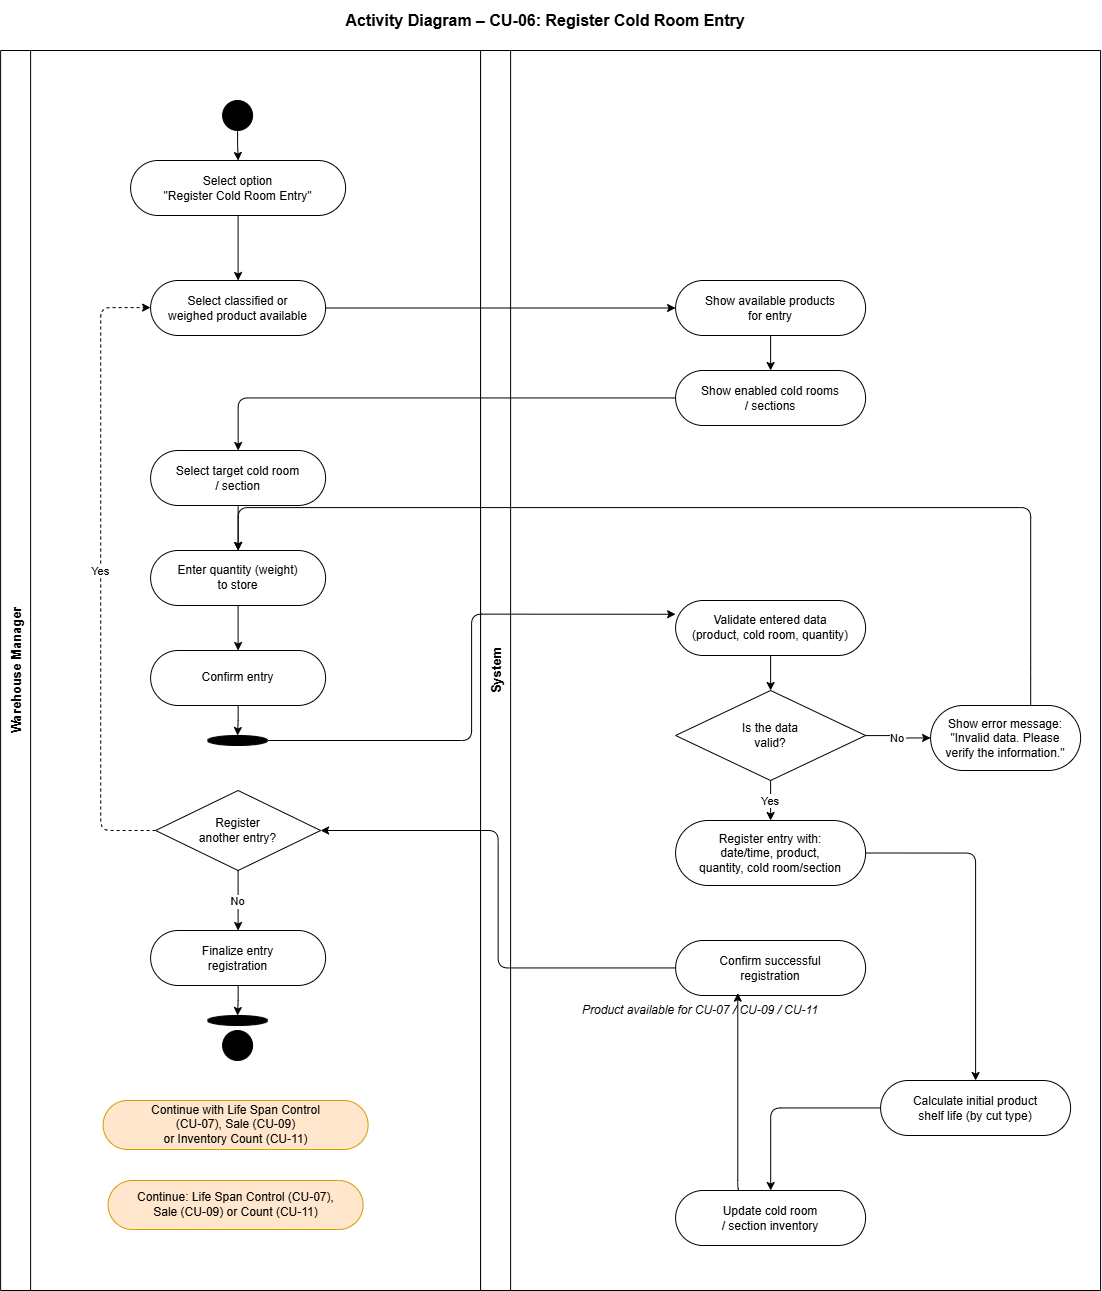
\includegraphics[width=\textwidth,keepaspectratio]{figures/06_Activity_Diagram_CU-06.png}
    \caption{Diagrama de actividad del CU-06}
    \label{fig:diagrama_clases}
\end{figure}

\subsection{Diagrama de estados}
La entidad con ciclo de vida no trivial es \texttt{ProductoAlmacenado}, con estados: \textit{Disponible} $\rightarrow$ \textit{Próximo a vencer} $\rightarrow$ \{\textit{Vendido} $\mid$ \textit{Dado de baja (pendiente de aprobación)} $\rightarrow$ \textit{Dado de baja (aprobado)}\} $\rightarrow$ \textit{Devuelto} (opcional, retorna a \textit{Disponible} o a \textit{Dado de baja} según el estado físico verificado).

\begin{figure}[H]
    \centering
    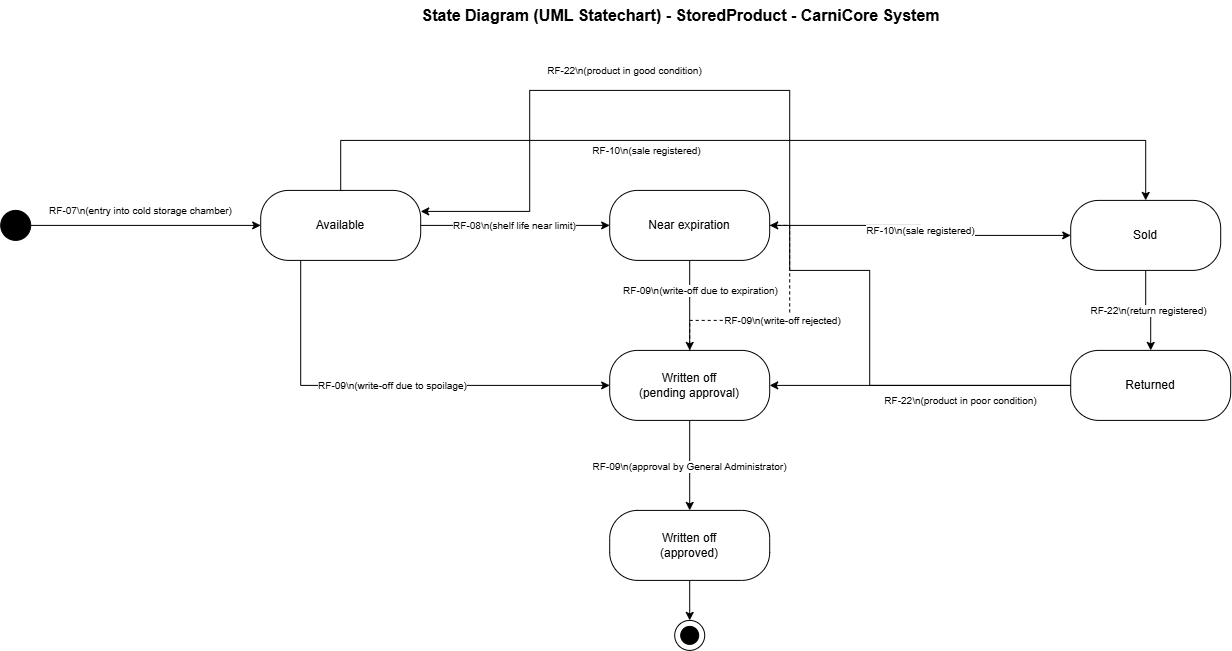
\includegraphics[width=0.7\textwidth,keepaspectratio]{figures/State_Diagram.png}
    \caption{Diagrama de estados del Sistema}
    \label{fig:diagrama_clases}
\end{figure}

\subsection{Diagrama de componentes}
\begin{figure}[H]
    \centering
    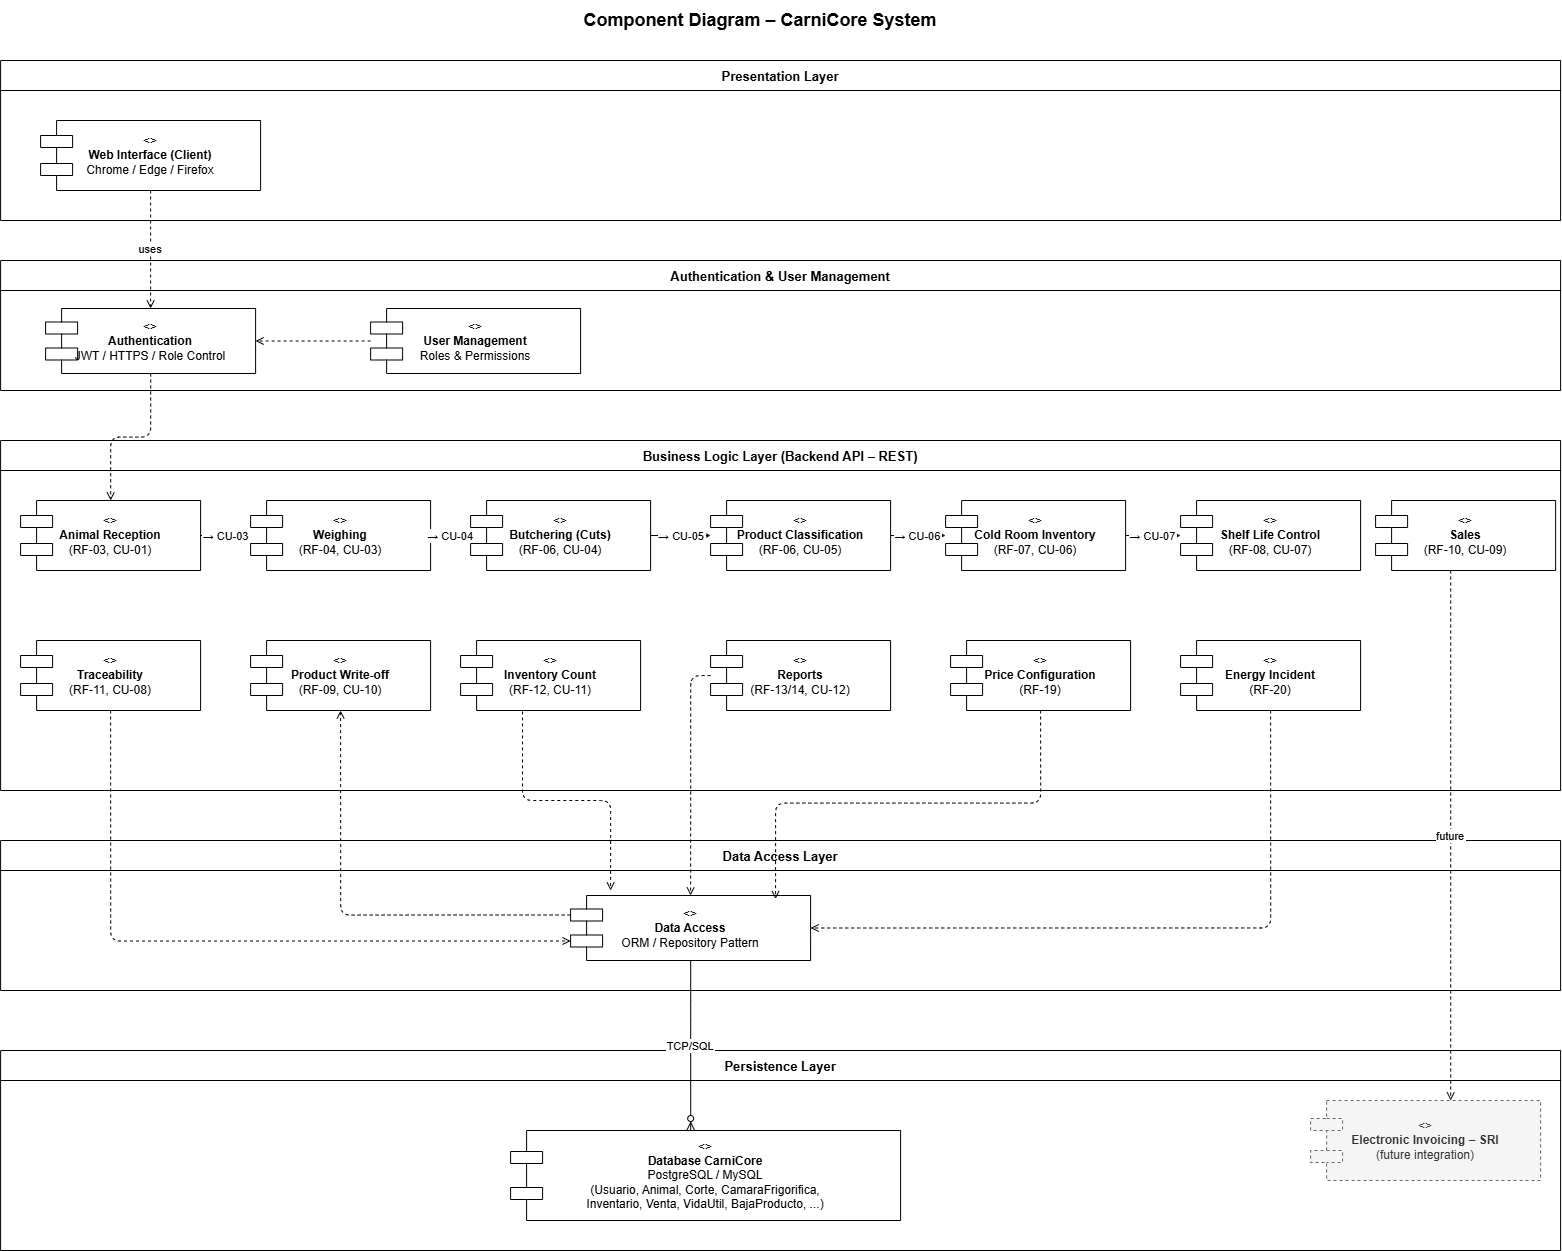
\includegraphics[width=\textwidth,keepaspectratio]{figures/Component_Diagram (2).png}
    \caption{Diagrama de componentes del Sistema}
    \label{fig:diagrama_clases}
\end{figure}

\subsection{Diagrama de despliegue}
\begin{figure}[H]
    \centering
    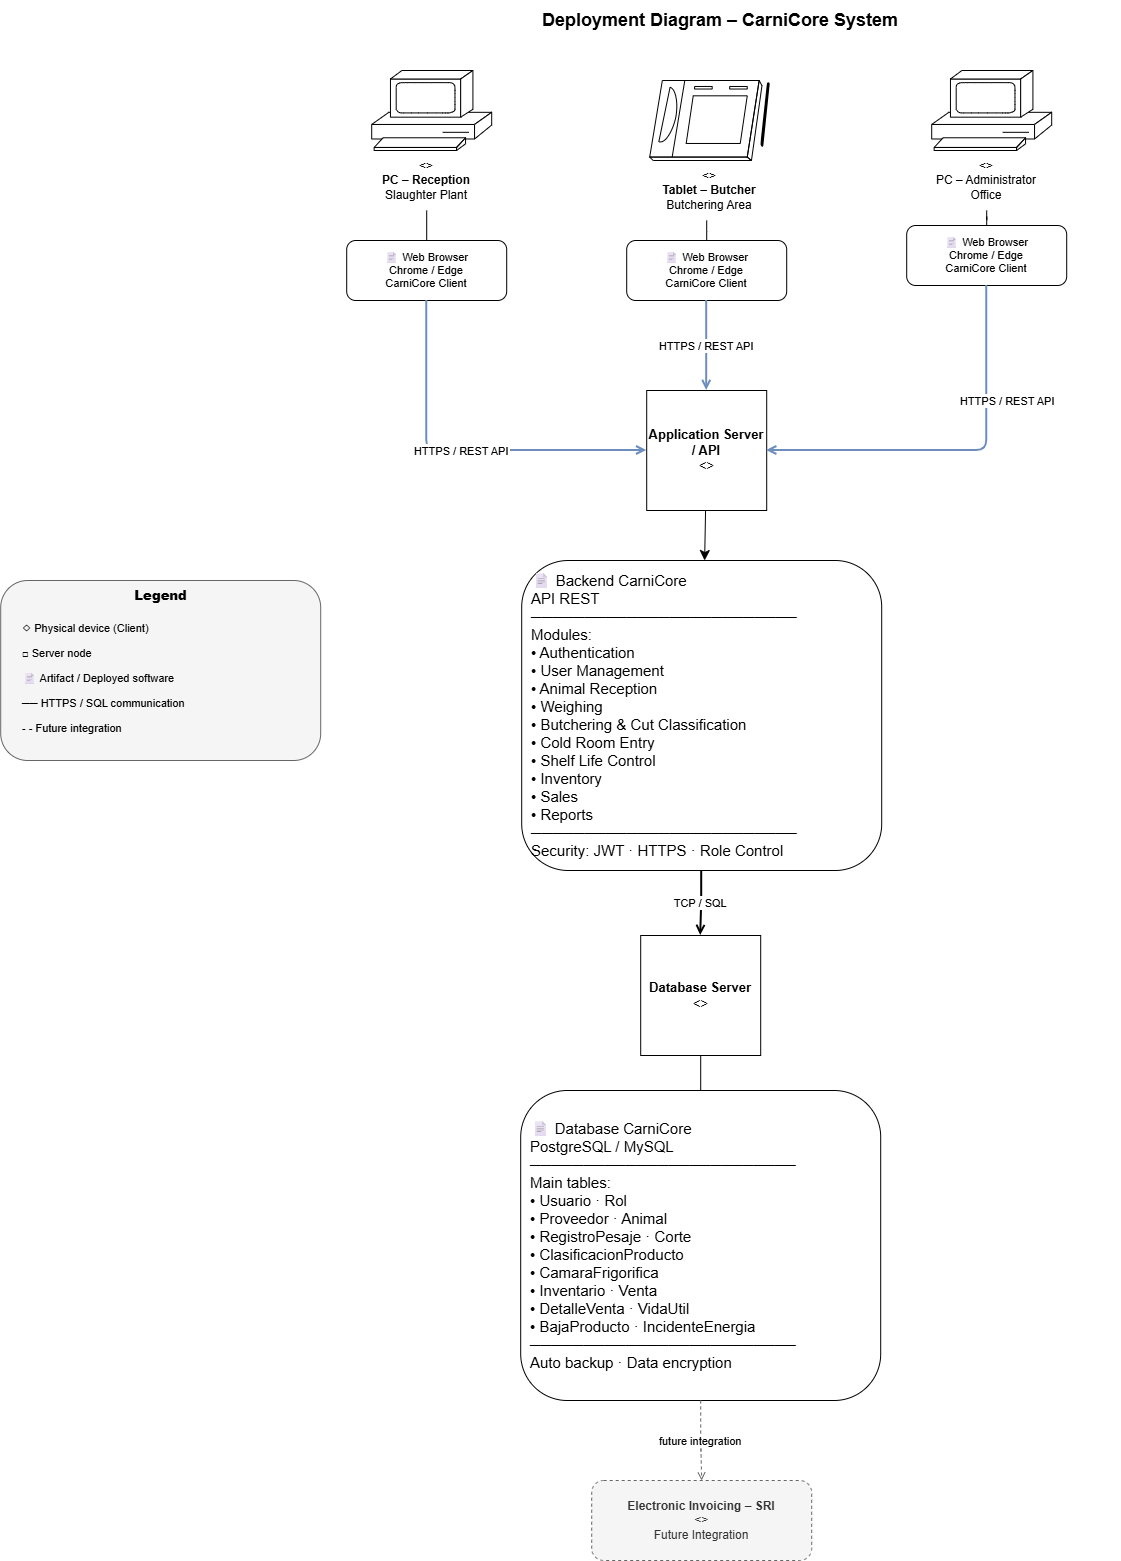
\includegraphics[width=0.9\textwidth,keepaspectratio]{figures/Deployement_Diagram (2).png}
    \caption{Diagrama de despliegue del Sistema}
    \label{fig:diagrama_clases}
\end{figure}

%======================================================
\section{Priorización y Trazabilidad Extendida}
%======================================================
\subsection{Priorización combinada MoSCoW + Kano + WSJF}
\begin{longtable}{|p{1.3cm}|p{1.8cm}|p{2.2cm}|p{1.6cm}|p{7.5cm}|}
\hline
\textbf{ID-RF} & \textbf{MoSCoW} & \textbf{Kano} & \textbf{WSJF*} & \textbf{Justificación breve} \\
\hline
RF-01 & Must & Básica & 8.0 & Sin proveedor regularizado no hay trazabilidad legal de origen. \\
RF-02 & Must & Básica & 8.0 & Exigencia directa de Agrocalidad; riesgo regulatorio si se omite. \\
RF-03 & Must & Básica & 8.0 & Núcleo operativo diario de bodega. \\
RF-04 & Must & Básica & 7.5 & Reemplaza el cálculo manual, fuente principal de errores actuales. \\
RF-05 & Should & Desempeño & 3.0 & Mejora la experiencia pero no bloquea la operación. \\
RF-06 & Must & Básica & 7.0 & Sin despiece registrado no hay inventario por corte. \\
RF-07 & Must & Básica & 7.0 & Base del control de inventario por cámara. \\
RF-08 & Must & Deleite/ Desempeño & 6.5 & Ataca directamente la pérdida por vencimiento reportada por la propietaria. \\
RF-09 & Must & Básica & 6.5 & Sustenta pérdidas con evidencia y control gerencial. \\
RF-10 & Must & Básica & 7.0 & Sin descuento automático el inventario queda desincronizado de las ventas. \\
RF-11 & Must & Deleite & 6.0 & Responde a auditorías de Agrocalidad en tiempo real. \\
RF-12 & Should & Desempeño & 2.5 & Mejora el control pero no es indispensable para operar. \\
RF-13 & Must & Desempeño & 5.5 & Insumo directo de decisiones gerenciales. \\
RF-14 & Should & Deleite & 2.0 & Valor agregado gerencial, no bloqueante. \\
RF-15 & Must & Básica & 6.0 & Seguridad y control de acceso mínimo viable. \\
RF-16 & Must & Básica & 5.5 & Permite auditar diferencias de inventario por fecha. \\
RF-17 & Should & Deleite & 1.5 & Enriquece la trazabilidad, no crítico. \\
RF-18 & Could & Indiferente & 1.0 & Consulta histórica de valor secundario. \\
RF-19 & Must & Desempeño & 5.0 & Necesario para operar cambios de precio sin intervención técnica. \\
RF-20 & Must & Deleite & 4.5 & Sustenta bajas por causa específica identificada en la entrevista (apagones). \\
RF-21 & Must & Básica & 6.0 & Requisito de continuidad operativa ante conectividad intermitente. \\
RF-22 & Should & Desempeño & 2.5 & Mejora el control de postventa. \\
RF-23 & Must & Deleite & 4.0 & Reduce tiempo de respuesta ante auditorías. \\
RF-24 & Should & Desempeño & 2.0 & Mejora la usabilidad operativa de bodega. \\
RF-25 & Could & Deleite & 1.0 & Diferenciador de cara al cliente final, no bloqueante. \\
\hline
\end{longtable}
\footnotesize{*WSJF estimado en escala relativa 0--10 (costo de retraso / tamaño estimado), a validar con el equipo completo y el \textit{product owner} antes del cierre de la Entrega 4.}

\textbf{Cálculo agregado del WSJF relativo (escala 0--10).} A partir de los 25 valores individuales de la tabla anterior, el equipo calculó los siguientes estadísticos por categoría MoSCoW, como insumo cuantitativo para ordenar el backlog del MVP (Sección~6):

\begin{longtable}{|p{2.2cm}|p{1.6cm}|p{2.2cm}|p{2.2cm}|p{2.2cm}|p{2.2cm}|}
\hline
\textbf{Categoría} & \textbf{N.° RF} & \textbf{WSJF total} & \textbf{WSJF promedio} & \textbf{WSJF mínimo} & \textbf{WSJF máximo} \\
\hline
Must & 17 & 108.0 & 6.35 & 4.0 (RF-23) & 8.0 (RF-01/02/03) \\
\hline
Should & 6 & 13.5 & 2.25 & 1.5 (RF-17) & 3.0 (RF-05) \\
\hline
Could & 2 & 2.0 & 1.0 & 1.0 (RF-18) & 1.0 (RF-25) \\
\hline
\textbf{Total} & \textbf{25} & \textbf{123.5} & \textbf{4.94} & -- & -- \\
\hline
\end{longtable}

El promedio de WSJF de la categoría \textit{Must} (6.35) casi triplica el de \textit{Should} (2.25), lo que confirma cuantitativamente la separación entre ambas categorías y respalda el orden de cobertura del MVP declarado en la Sección~6 (RF-01 a RF-04 como primer bloque por WSJF $\geq 7.5$). Estas estimaciones se mantienen en escala relativa 0--10 (costo de retraso / tamaño estimado, sin descomponer aún en t-shirt sizing ni puntos de historia); la descomposición formal en valor de negocio, criticidad temporal y reducción de riesgo, junto con su validación explícita con la propietaria, queda planificada para la Entrega 4 (2B), sin que ello impida su uso como criterio de ordenamiento en la presente entrega.

\subsection{Matriz de trazabilidad extendida (40 filas)}
Enlaza: Ley/Artículo $\to$ Objetivo $\to$ Interesado $\to$ ID-EV $\to$ RF/RNF $\to$ CU $\to$ HU $\to$ CA $\to$ Componente $\to$ Mockup.

\scriptsize
\begin{longtable}{|p{0.5cm}|p{1.5cm}|p{2.2cm}|p{1.5cm}|p{0.8cm}|p{0.8cm}|p{0.8cm}|p{0.8cm}|p{0.8cm}|p{1.3cm}|p{1cm}|}
\hline
\textbf{ID} & \textbf{Ley-Art.} & \textbf{Objetivo} & \textbf{Interesado} & \textbf{EV} & \textbf{RF/RNF} & \textbf{CU} & \textbf{HU} & \textbf{CA} & \textbf{Componente} & \textbf{Mockup} \\
\hline
1 & -- & Trazabilidad de origen & Propietaria & EV-01 & RF-01 & CU-01 & HU-01 & CA-01 & Backend-Proveedores & MU-02 \\
2 & Art.30 & Certificación sanitaria & Propietaria & EV-02 & RF-02 & CU-02 & HU-02 & CA-02 & Backend-Guias & MU-02 \\
3 & -- & Registro de ingreso & Bodega & EV-03 & RF-03 & CU-01 & HU-03 & CA-03 & Backend-Ingresos & MU-02 \\
4 & -- & Cálculo de costo & Bodega & EV-04 & RF-04 & CU-03 & HU-04 & CA-04 & Backend-Pesaje & MU-03 \\
5 & -- & Comprobante físico & Bodega & EV-04 & RF-05 & CU-03 & -- & -- & Backend-Pesaje & MU-03 \\
6 & -- & Registro de cortes & Carniceros & EV-05 & RF-06 & CU-04 & HU-06 & CA-06 & Backend-Despiece & -- \\
7 & -- & Control por cámara & Admin. gral. & EV-06 & RF-07 & CU-06 & HU-07 & CA-07 & Backend-Inventario & MU-04 \\
8 & -- & Evitar pérdidas & Admin. gral. & EV-06 & RF-08 & CU-07 & HU-08 & CA-08 & Backend-VidaUtil & MU-04 \\
9 & Art.38 & Sustentar bajas & Admin. gral. & EV-07 & RF-09 & CU-10 & HU-09 & CA-09 & Backend-Bajas & -- \\
10 & -- & Registrar ventas & Bodega/Cliente & EV-08 & RF-10 & CU-09 & HU-10 & CA-10 & Backend-Ventas & -- \\
11 & -- & Historial completo & Agrocalidad/Prop. & EV-03 & RF-11 & CU-08 & HU-11 & CA-11 & Backend-Trazabilidad & MU-06 \\
12 & -- & Diferencias de inventario & Admin. gral. & EV-09 & RF-12 & CU-11 & -- & -- & Backend-Inventario & -- \\
13 & -- & Decisiones gerenciales & Propietaria & EV-08 & RF-13 & CU-12 & HU-13 & CA-13 & Backend-Reportes & MU-05 \\
14 & -- & Desempeño del negocio & Propietaria & EV-08 & RF-14 & CU-12 & -- & -- & Backend-Reportes & MU-05 \\
15 & Art.7,9 & Delegar por rol & Propietaria & EV-01 & RF-15 & -- & HU-15 & CA-15 & Backend-Usuarios & MU-01 \\
16 & -- & Stock por fecha & Propietaria & EV-09 & RF-16 & CU-06 & HU-16 & CA-16 & Backend-Inventario & -- \\
17 & -- & Georreferencia & Admin. gral. & EV-10 & RF-17 & CU-01 & -- & -- & Backend-Proveedores & MU-04 \\
18 & -- & Historial de precios & Propietaria & EV-11 & RF-18 & -- & -- & -- & Backend-Precios & MU-14 \\
19 & -- & Configurar precios & Propietaria & EV-11 & RF-19 & CU-03 & HU-19 & CA-19 & Backend-Precios & MU-14 \\
20 & -- & Registrar apagones & Propietaria & EV-12 & RF-20 & CU-10 & HU-20 & CA-20 & Backend-Incidentes & -- \\
21 & -- & Continuidad operativa & Bodega & EV-13 & RF-21 & CU-01/CU-03 & HU-21 & CA-21 & Cliente-Offline & -- \\
22 & -- & Devoluciones & Bodega & EV-14 & RF-22 & CU-09 & -- & -- & Backend-Ventas & MU-14 \\
23 & -- & Auditoría Agrocalidad & Admin. gral. & EV-15 & RF-23 & CU-08 & HU-23 & CA-23 & Backend-Trazabilidad & MU-16 \\
24 & -- & Búsqueda de producto & Bodega & EV-09 & RF-24 & CU-06 & -- & -- & Backend-Inventario & MU-10 \\
25 & -- & QR de trazabilidad & Cliente & EV-03 & RF-25 & CU-08 & -- & -- & Backend-Trazabilidad & MU-16 \\
26 & -- & Rendimiento del pesaje & Bodega & EV-04 & RNF-01 & CU-03 & -- & -- & Backend-Pesaje & -- \\
27 & -- & Disponibilidad del servicio & Todos & EV-20 & RNF-02 & -- & -- & -- & Infraestructura & -- \\
28 & Art.30 & Autenticación segura & Admin. gral. & EV-01 & RNF-03 & -- & -- & -- & Backend-Usuarios & -- \\
29 & -- & Usabilidad de bodega & Bodega & EV-09 & RNF-04 & CU-01 & -- & -- & Cliente-Web/Móvil & -- \\
30 & -- & Arquitectura mantenible & Equipo técnico & -- & RNF-05 & -- & -- & -- & Backend (todos) & -- \\
31 & -- & Acceso multi-navegador & Todos & -- & RNF-06 & -- & -- & -- & Cliente-Web & -- \\
32 & Art.38 & Auditoría de bajas & Admin. gral. & EV-07 & RNF-07 & CU-10 & -- & -- & Backend-Bajas & -- \\
33 & -- & Cobertura RF Must en MVP & Docente/Equipo & EV-16 & RNF-08 & -- & -- & -- & MVP & -- \\
34 & -- & Integración con báscula & Bodega & -- & RNF-09 & CU-03 & -- & -- & Backend-Pesaje & -- \\
35 & -- & Nuevos tipos de producto & Propietaria & EV-11 & RNF-10 & -- & -- & -- & Backend-Precios & -- \\
36 & -- & Reportes con alto volumen & Propietaria & EV-08 & RNF-11 & CU-12 & -- & -- & Backend-Reportes & -- \\
37 & Art.30 & Cifrado de datos personales & Todos & -- & RNF-12 & -- & -- & -- & Backend/BD & -- \\
38 & -- & Accesibilidad táctil & Bodega & EV-09 & RNF-13 & CU-01 & -- & -- & Cliente-Móvil & -- \\
39 & -- & Recuperabilidad offline & Bodega & EV-13 & RNF-14 & CU-01/CU-03 & HU-21 & CA-21 & Cliente-Offline & -- \\
40 & -- & Calidad del código MVP & Docente/Equipo & EV-16 & RNF-15 & -- & -- & -- & MVP & -- \\
\hline
\end{longtable}
\normalsize

%======================================================
\section{Producto Mínimo Viable (MVP)}
%======================================================
El MVP de CarniCore se aloja en el repositorio del trabajo en la carpeta 
\texttt{05\_MVP/Ejecutable/Carnicore}, donde se pueden observar todas las 
carpetas y archivos tanto para el frontend como para el backend del mismo, 
contando con un \texttt{README.md} de instrucciones para levantar el programa 
y un \texttt{video\_demo.mp4} tutorial del mismo. 

\noindent El MVP debe cubre al menos el 60\% de los RF listados en 
la Sección~5.1 (RF-01, 02, 03, 04, 06, 07, 08, 09, 10, 11, 13, 15, 16, 19, 20, 
21, 23; total 17 RF Must, de los cuales al menos 11 están cubiertos).

%======================================================
\section{Componente Empírico -- Diseño del Estudio}
%======================================================
El equipo declara que trabajará con el \textbf{Enfoque~2 -- Detección automática de ambigüedad y malos olores en los requisitos}, aplicado sobre el conjunto de 25 RF de la Sección~3.2, dado que es el enfoque más directamente derivable del propio ERS sin depender de la disponibilidad de personal experto externo para una evaluación comparativa con LLM.

\subsection{Pregunta de investigación (PICOC)}
\begin{itemize}[nosep]
\item \textbf{Población:} el conjunto de 25 requisitos funcionales elicitados para CarniCore.
\item \textbf{Intervención:} un detector automático de ambigüedad y malos olores (cuantificadores vagos, conjunciones múltiples, voz pasiva), implementado con expresiones regulares en Python o con la herramienta \texttt{smella} de Ferrari et al.
\item \textbf{Comparación:} el juicio consensuado de al menos tres personas expertas que clasifican cada RF como ``ambiguo'' o ``no ambiguo'' sin ver la salida del detector.
\item \textbf{Resultado:} precisión, exhaustividad (\textit{recall}) y medida F1 del detector respecto al consenso experto; acuerdo inter-evaluador $\kappa$ de Cohen \cite{cohen1960kappa} y $\kappa$ de Fleiss \cite{fleiss1971kappa}.
\item \textbf{Contexto:} un proyecto académico de ingeniería de requisitos aplicado a un dominio real de distribución cárnica en Ecuador.
\end{itemize}

\textbf{RQ1:} ¿Con qué precisión un detector automático replica el juicio de personas expertas al identificar RF ambiguos en el conjunto de requisitos de CarniCore?

\subsection{Elementos del protocolo experimental}
El protocolo experimental completo del Enfoque~2 se encuentra versionado en 06\_Experimento/protocolo.pdf (v1.0, 02/08/2026); a continuación se resumen sus elementos conforme a la Sección~5 de la guía. El registro previo del protocolo se completó en OSF el 02/08/2026 (\url{https://osf.io/wud69}), con fecha anterior a toda recolección de datos.

\textbf{Diseño.} Estudio observacional de exactitud diagnóstica (\textit{diagnostic accuracy study}), transversal y censal: se aplican dos procedimientos de clasificación (detector automático; consenso experto) sobre la misma población completa de 25 RF, sin asignación aleatoria ni manipulación de condiciones. La unidad de análisis es el RF individual (RF-01 a RF-25). Las personas expertas clasifican de forma ciega e independiente, sin conocer la salida del detector ni las clasificaciones de las demás personas expertas.

\textbf{Hipótesis.} Formuladas sobre el nivel de acuerdo (\(\kappa\) de Cohen) entre el detector y el consenso experto:
\begin{itemize}[nosep]
\item \(H_0\): el acuerdo entre el detector automático y el consenso experto no supera el nivel esperable por azar (\(\kappa \leq 0\)); equivalentemente, la medida F1 del detector no difiere de la que produciría una clasificación aleatoria con la misma prevalencia de RF ambiguos observada en el consenso experto.
\item \(H_1\): el acuerdo entre el detector automático y el consenso experto es significativamente superior al nivel esperable por azar (\(\kappa > 0\)).
\end{itemize}
Dado el tamaño reducido de la población (25 RF), el estudio se reporta con énfasis en el tamaño del efecto (\(\kappa\), precisión, \textit{recall}, F1) y no únicamente en la significancia estadística \cite{wohlin2012experimentation}.

\textbf{Variables.}
\begin{itemize}[nosep]
\item \textit{Agrupación (fuente de clasificación):} dos niveles -- (a) salida del detector automático, (b) consenso de personas expertas.
\item \textit{Dependiente primaria:} clasificación binaria de cada RF (ambiguo / no ambiguo) emitida por cada fuente.
\item \textit{Dependientes derivadas:} precisión, \textit{recall} y F1 del detector respecto al consenso experto; \(\kappa\) de Cohen por par de expertos; \(\kappa\) de Fleiss para el conjunto de expertos.
\item \textit{De control:} mismo conjunto congelado de 25 RF; expertos ciegos entre sí y ciegos a la salida del detector; misma ventana temporal de aplicación; misma definición operativa de ambigüedad para todas las partes; orden de presentación de los RF aleatorizado por evaluador con semilla fija (\texttt{seed = 42 + índice\_evaluador}).
\item \textit{Extrañas reconocidas:} experiencia previa de cada persona experta en redacción de requisitos y posible familiaridad con el dominio cárnico, documentadas en la ficha de perfil del experto.
\end{itemize}

\textbf{Población y muestra.} Censo completo de los 25 RF del ERS/SRS v3.0 (RF-01 a RF-25); no se aplica muestreo probabilístico. Mínimo 3 personas expertas evaluadoras (recomendado 5), sin pertenecer al equipo CarniCore, con formación o experiencia en ingeniería de requisitos o de software. El conjunto de 25 RF solo se congela para clasificación una vez que las evidencias EV-17 a EV-25 estén respaldadas por evidencia real de campo.

\textbf{Instrumentos.}
\begin{itemize}[nosep]
\item \textit{Detector automático} de ambigüedad y malos olores (cuantificadores vagos, conjunciones múltiples, voz pasiva sin agente explícito), implementado como script propio en Python mediante expresiones regulares por categoría, congelado en versión 1.0 antes de la ejecución (\texttt{06\_Experimento/scripts\_analisis/detector\_ambiguedad.py}); el uso de un modelo de lenguaje como apoyo técnico de prototipado del detector se documenta íntegramente en \texttt{06\_Experimento/prompts\_llm/} (prompt exacto, modelo, temperatura, \textit{top-p} y semilla), sin que el modelo participe en la clasificación experta.
\item \textit{Rúbrica de clasificación experta}: instrumento binario (ambiguo / no ambiguo) con categoría de ambigüedad, aplicado de forma individual e independiente a cada uno de los 25 RF, con una definición operativa única de ambigüedad compartida por todas las personas expertas y escala de confianza Likert 1--5.
\item \textit{Ficha de perfil} de la persona experta (código de participante, años de experiencia, rol, vínculo institucional), sin datos identificables.
\item \textit{Consentimiento informado} adaptado del paquete ético ya aprobado 

(\texttt{08\_Etica/A03\_Consentimiento\_Informado.pdf}) para el rol de persona evaluadora experta, incluyendo la cláusula de uso de la clasificación en publicaciones revisadas por pares y en el conjunto de datos anónimo depositado en Zenodo bajo licencia CC~BY~4.0.
\end{itemize}

\textbf{Procedimiento (seis pasos).} (1) Selección y congelamiento del detector; (2) ejecución del detector sobre los 25 RF, con registro del resultado crudo; (3) clasificación experta ciega e independiente de los 25 RF por al menos tres personas expertas; (4) cálculo de precisión, \textit{recall} y F1 del detector frente al consenso experto (mayoría simple; los empates se registran como desacuerdo no resuelto); (5) cálculo del acuerdo inter-evaluador (\(\kappa\) de Cohen por par de expertos y \(\kappa\) de Fleiss para el conjunto); (6) discusión de desacuerdos detector--consenso, con una nota breve por caso. Todos los artefactos intermedios se versionan en \texttt{06\_Experimento/resultados/} y \texttt{06\_Experimento/scripts\_analisis/} para asegurar reproducibilidad.

\textbf{Plan de análisis estadístico.} Estadística descriptiva de las clasificaciones y matriz de confusión; cálculo de precisión, \textit{recall} y F1 con intervalos de confianza aproximados; \(\kappa\) de Cohen por par de expertos y \(\kappa\) de Fleiss para el conjunto, con interpretación cualitativa del nivel de acuerdo. Al tratarse de una variable categórica binaria pareada sobre una población censal pequeña, no se aplica la prueba de normalidad de Shapiro--Wilk (reservada para variables continuas); en su lugar se evalúa si \(\kappa\) difiere significativamente de cero mediante su error estándar asintótico, fijando \(\alpha = 0{,}05\). Si en una versión posterior se incorporan puntuaciones continuas (por ejemplo, nivel de confianza), se aplicará Shapiro--Wilk antes de elegir entre pruebas paramétricas y no paramétricas. Ante múltiples \(\kappa\) pareados se aplica corrección de Bonferroni. El análisis se implementa en Python (\texttt{scikit-learn} para precisión/\textit{recall}/F1; \texttt{statsmodels.stats.inter\_rater} para los coeficientes \(\kappa\)), en \texttt{06\_Experimento/scripts\_analisis/analisis\_kappa\_f1.py}, con versiones de librerías congeladas en \texttt{requirements.txt}.

\textbf{Consideraciones éticas.} El estudio opera bajo la categoría de riesgo C (riesgo mínimo operativo) y los límites de uso de IA declarados en la Sección~4 de la Adenda Ética de la Segunda Ronda. No se recolecta ningún dato personal identificable de las personas expertas más allá de un código de participante. Como precondición de ejecución (\textit{gatekeeper} G8), la Adenda Ética de la Segunda Ronda debe estar firmada y con las cifras de participantes por rol completas antes de recabar el primer consentimiento de persona experta.

%======================================================
\section{Puente hacia la Entrega 4 -- Preparación de la publicación}
%======================================================
\textbf{Título y resumen preliminar del manuscrito.} Borrador v1.0 en 

\texttt{07\_Publicacion/manuscrito\_borrador.pdf} (02/08/2026, no enviado a ninguna revista):

\begin{quote}
\small
\textit{``Detección automática de patrones de ambigüedad en requisitos funcionales: un estudio exploratorio en el dominio de trazabilidad cárnica''}
\end{quote}

\textbf{Contexto.} La ambigüedad textual en los requisitos es una causa documentada de retrabajo y de malentendidos entre partes interesadas. \textbf{Objetivo.} Caracterizar la presencia de patrones léxico-sintácticos de ambigüedad (cuantificadores vagos, conjunciones múltiples, voz pasiva sin agente explícito) en el conjunto completo de RF de CarniCore. \textbf{Método.} Se ejecutó el detector de expresiones regulares (tres categorías de patrón) sobre los 25 RF verbatim del ERS/SRS v3.0, población completa, sin muestreo. \textbf{Resultados.} El detector no activó ninguna categoría en ninguno de los 25 RF (0/25, 0\,\%). \textbf{Conclusiones.} El hallazgo es consistente con un estilo de redacción homogéneo, pero no permite concluir ausencia de ambigüedad en sentido amplio, ya que el detector cubre solo ambigüedad léxica y sintáctica superficial, no semántica ni pragmática.

El borrador deja explícitamente \textbf{fuera de alcance} en esta entrega la comparación contra un panel de personas expertas (Secciones~3 y~7--8 del manuscrito): el equipo no contó con acceso a evaluadores externos independientes durante el periodo de esta entrega, por lo que esa validación no se simula ni se estima, y el diseño comparativo completo permanece pre-registrado en OSF (\url{https://osf.io/wud69}) para una fase posterior. En consecuencia, el manuscrito no reporta ninguna cifra de precisión, \textit{recall}, F1 ni $\kappa$ en esta versión, conforme a la advertencia de la guía sobre fabricación de evidencia (\textit{gatekeeper} G4); la introducción, el trabajo relacionado y la metodología (Secciones~1--4) están cerrados, y las Secciones~5--8 (resultados, discusión, amenazas a la validez y trabajo futuro) reportan únicamente la evidencia primaria real disponible a la fecha.

\textbf{Búsqueda de revista objetivo.} Documentada en \texttt{07\_Publicacion/analisis\_revistas.md} (búsqueda del 02/08/2026, en los sitios oficiales de cada editorial y en SCImago Journal Rank). Tres candidatas evaluadas, una por editorial:

\begin{itemize}[nosep]
\item \textbf{Requirements Engineering} (Springer, híbrida): SJR 0,798 (Q2); encaje temático alto (ambigüedad de requisitos), aunque exigente en tamaño de muestra y validación industrial para un artículo completo. \textbf{Primera opción}, en modalidad de \textit{short paper} o nota de investigación.
\item \textbf{Journal of Systems and Software} (Elsevier, híbrida): SJR 0,975 (Q1 en Hardware and Architecture, Information Systems y Software); APC de USD~3.670 si se opta por acceso abierto, sin costo vía suscripción; exige evidencia empírica de cualquier tipo, no solo industrial a gran escala. \textbf{Segunda opción.}
\item \textbf{IEEE Transactions on Software Engineering} (IEEE, híbrida): Q1, factor de impacto 6,5 (2023); APC de USD~2.800 (envíos 2026) si se opta por acceso abierto, sin costo vía suscripción. Prestigio muy alto pero exige mayor escala y rigor estadístico que un estudio con 25 RF; \textbf{no recomendada como primer destino} para este tamaño de estudio, se reserva como objetivo de mediano plazo.
\end{itemize}

Ruta de bajo costo si no hay fondos para APC: publicar en modalidad de suscripción (sin pago) en cualquiera de las tres y depositar el manuscrito en Zenodo, verificando antes la política de auto-archivo de cada editorial en Sherpa/RoMEO.

\textbf{Licencia del paquete de datos.} Definida en \texttt{07\_Publicacion/dataset\_zenodo/LICENSE.txt}: Creative Commons Atribución 4.0 Internacional (CC~BY~4.0), que permite compartir y adaptar el conjunto de datos, incluso comercialmente, bajo atribución adecuada y sin restricciones legales o técnicas adicionales sobre lo que la licencia ya permite. El archivo incluye el enlace al texto legal completo y al resumen legible (\url{https://creativecommons.org/licenses/by/4.0/legalcode} y \url{/deed.es}), y una cita provisional del conjunto de datos en formato APA, pendiente únicamente de completar con el DOI real que Zenodo asigne al momento del depósito.

%======================================================
\appendix
\section{Plan del proyecto de Ingeniería de Requisitos}
%======================================================
\subsection{Identificación de stakeholders}
Véase la Sección~2.3 (mapa de interesados y matriz poder/interés), que actualiza y reemplaza la tabla simplificada de la Entrega 1B.

\subsection{Cronograma de actividades de IR (actualizado a la Entrega 3)}
\begin{longtable}{|p{1.6cm}|p{8.5cm}|p{3.5cm}|}
\hline
\textbf{Semana} & \textbf{Actividad} & \textbf{Responsable} \\
\hline
1--10 & Actividades de la Entrega 1A y 1B (elicitación inicial, mockups, RF/RNF parciales, CU y clases parciales). & Todo el equipo \\
\hline
11 & Adenda ética de la segunda ronda; diseño experimental; registro del protocolo en OSF. & Verificador / Analista líder \\
\hline
12 & Ejecución de la segunda ronda de campo (mínimo 8 entrevistas nuevas); cuestionario ampliado; validación piloto. & Todo el equipo \\
\hline
13 & Consolidación del ERS/SRS completo (esta versión) y del MVP; entrega 2A. & Todo el equipo \\
\hline
14--17 & Análisis de datos, borrador y versión final del manuscrito, depósito en Zenodo y defensa. & Todo el equipo \\
\hline
\end{longtable}

\subsection{Técnicas de elicitación seleccionadas y justificación}
Se mantiene la entrevista semiestructurada como técnica principal (justificación heredada de la Entrega 1B), complementada en esta entrega con observación directa de los procesos de pesaje y despiece en la planta de La Maná y con un cuestionario aplicado a al menos tres perfiles de usuario, para validar y refinar en particular RNF-04 (usabilidad) y RNF-14 (recuperabilidad offline).

%======================================================
\section{Evidencias de elicitación}
%======================================================

\subsection{Intrumento de recolección de datos (guía entrevista)}
\begin{figure}[H]
    \centering
    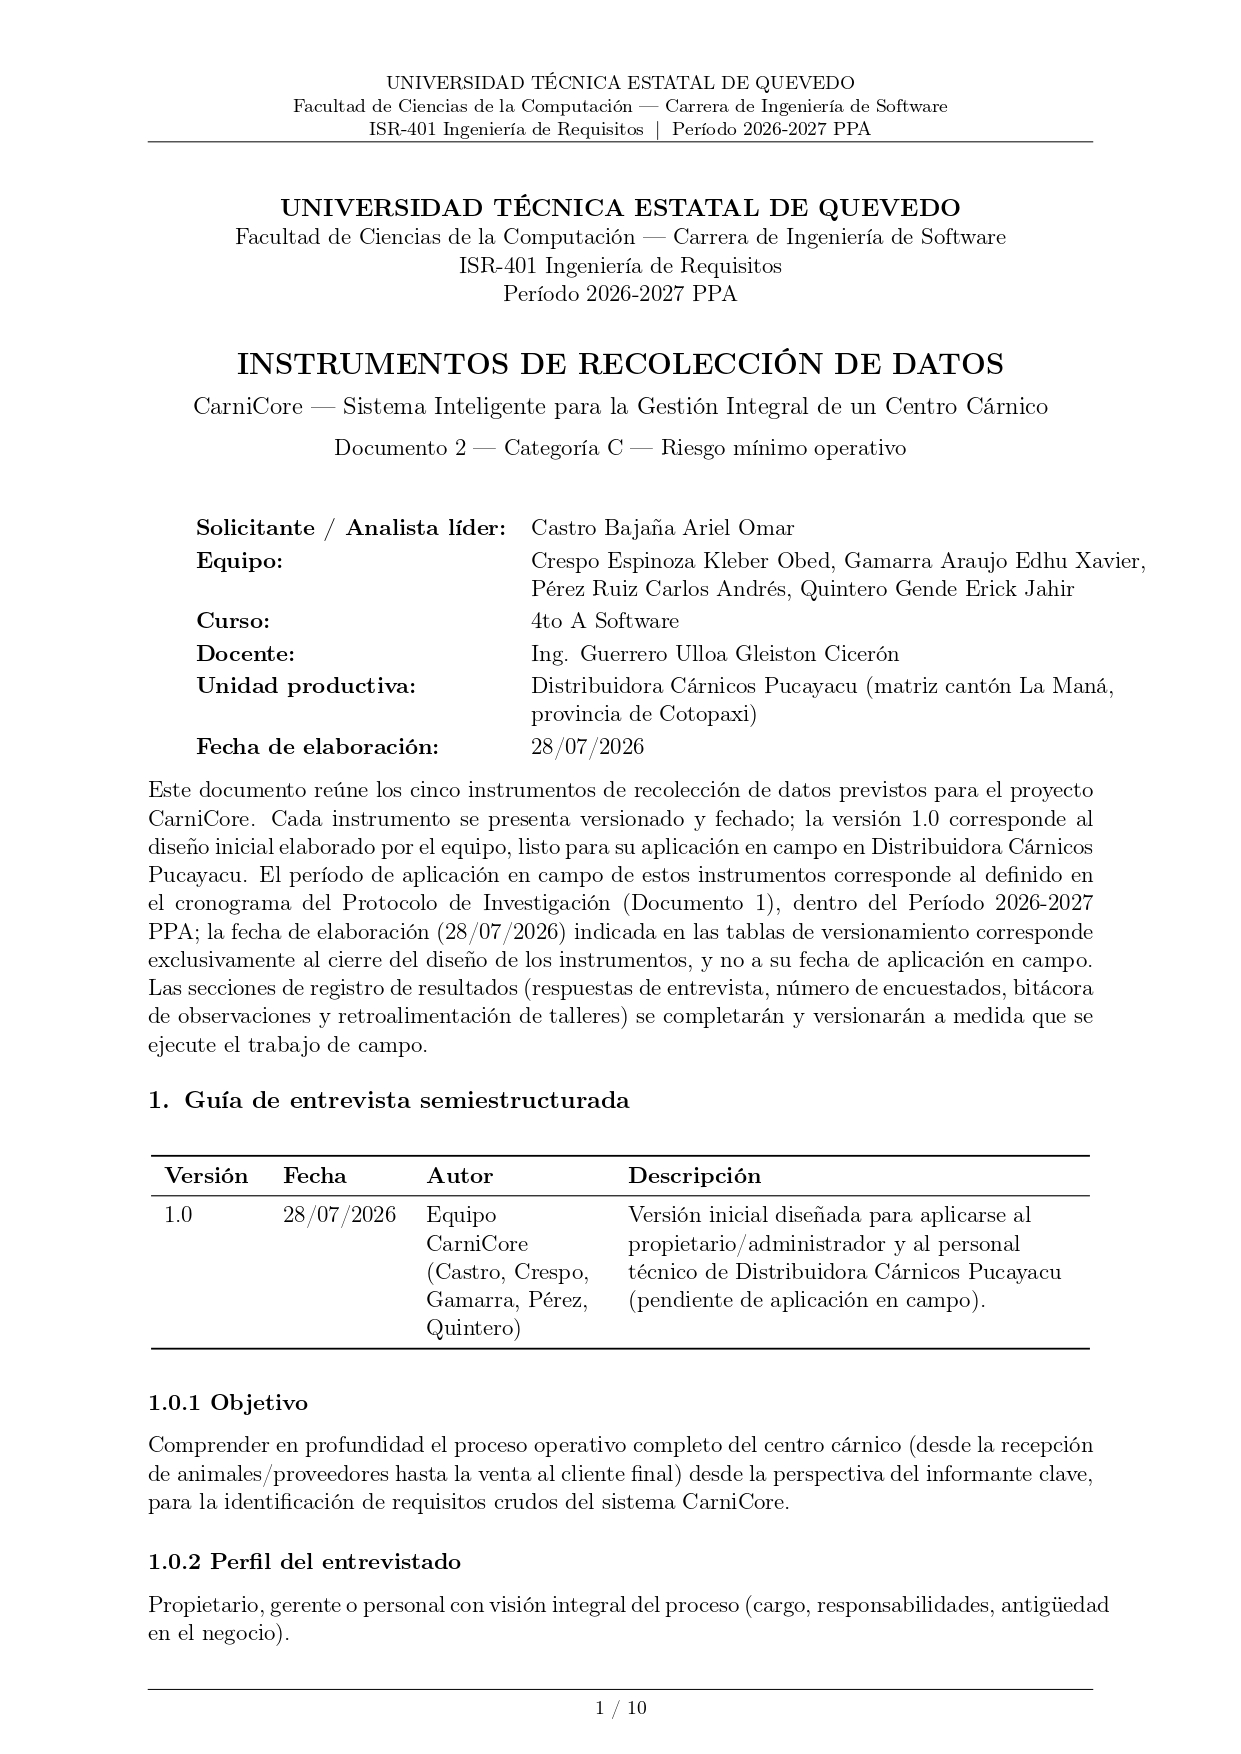
\includegraphics[width=\textwidth,keepaspectratio]{figures/A02_Instrumentos_Recoleccion_page-0001.jpg}
    \label{fig:diagrama_clases}
\end{figure}

\begin{figure}[H]
    \centering
    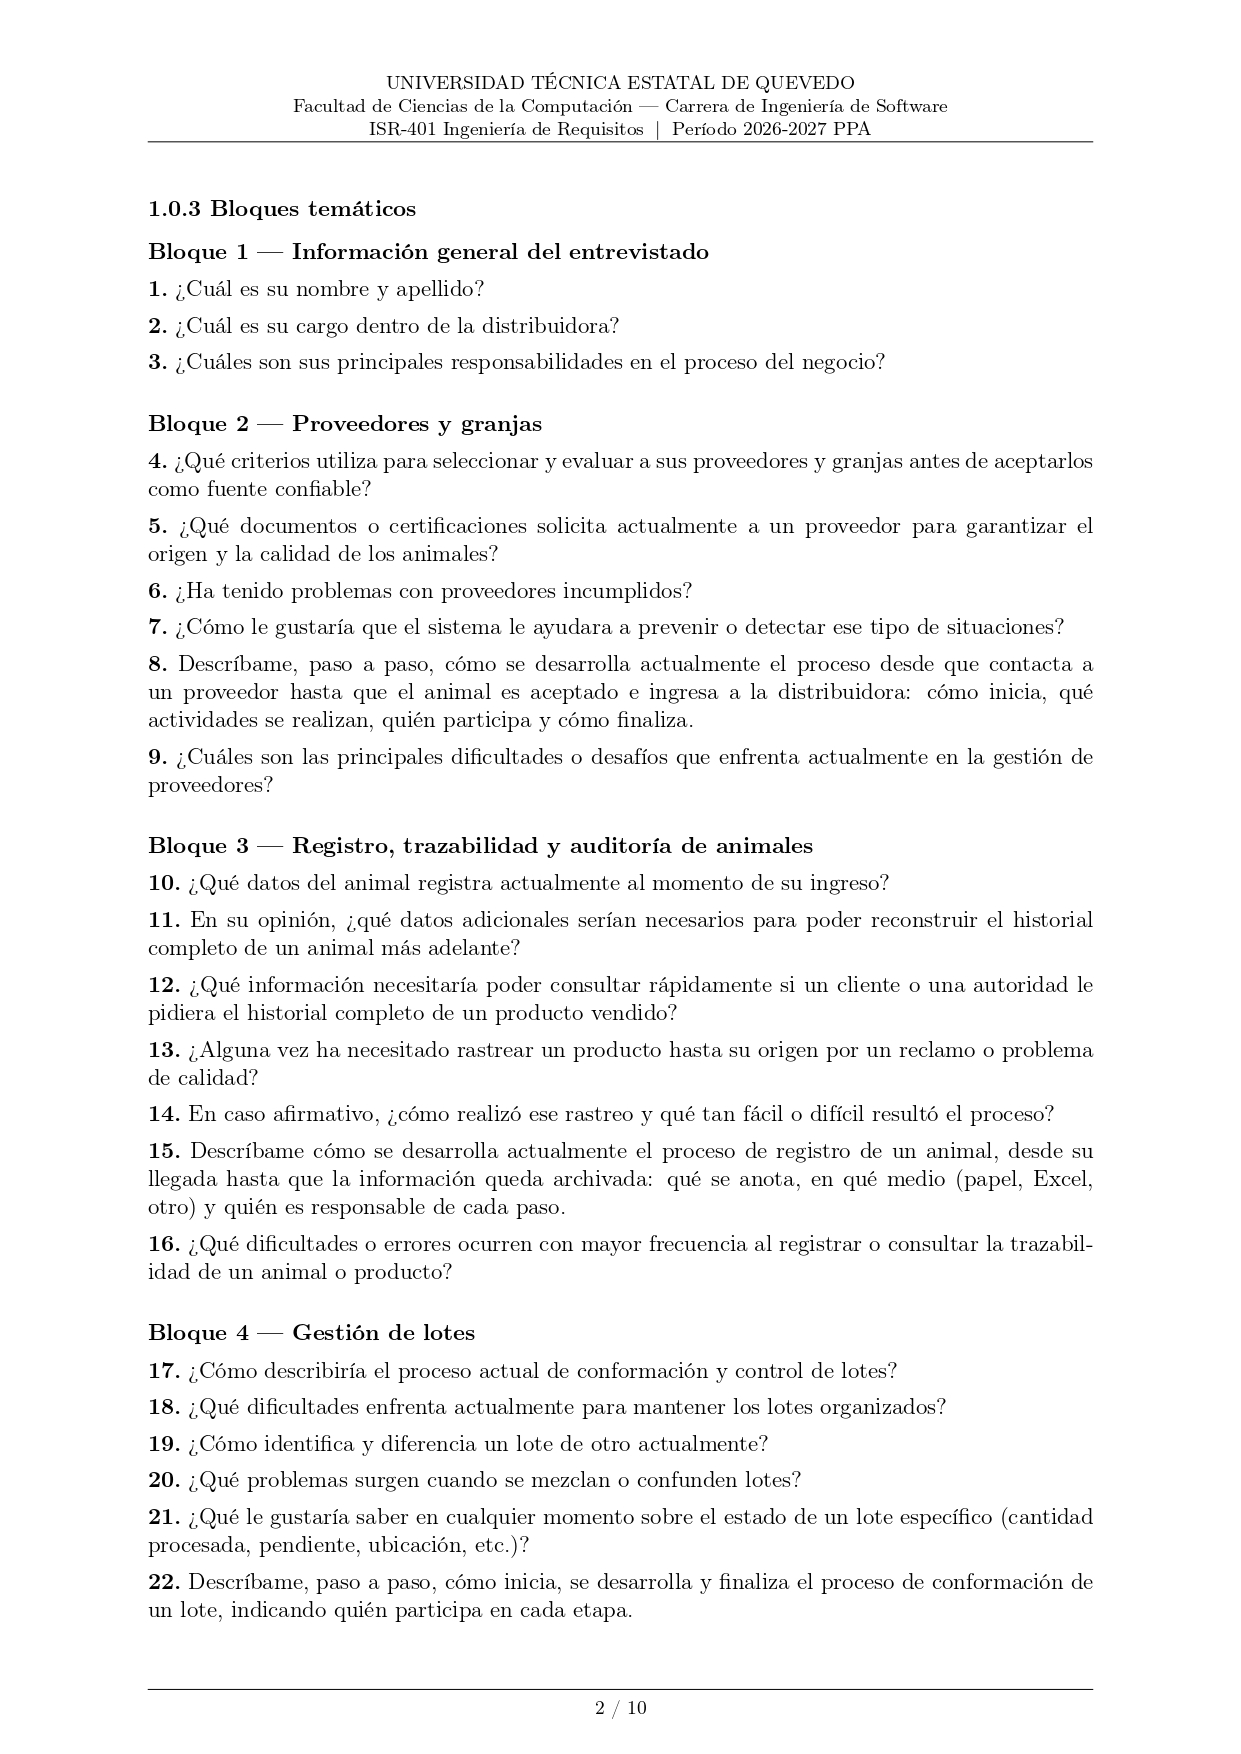
\includegraphics[width=\textwidth,keepaspectratio]{figures/A02_Instrumentos_Recoleccion_page-0002.jpg}
    \label{fig:diagrama_clases}
\end{figure}

\begin{figure}[H]
    \centering
    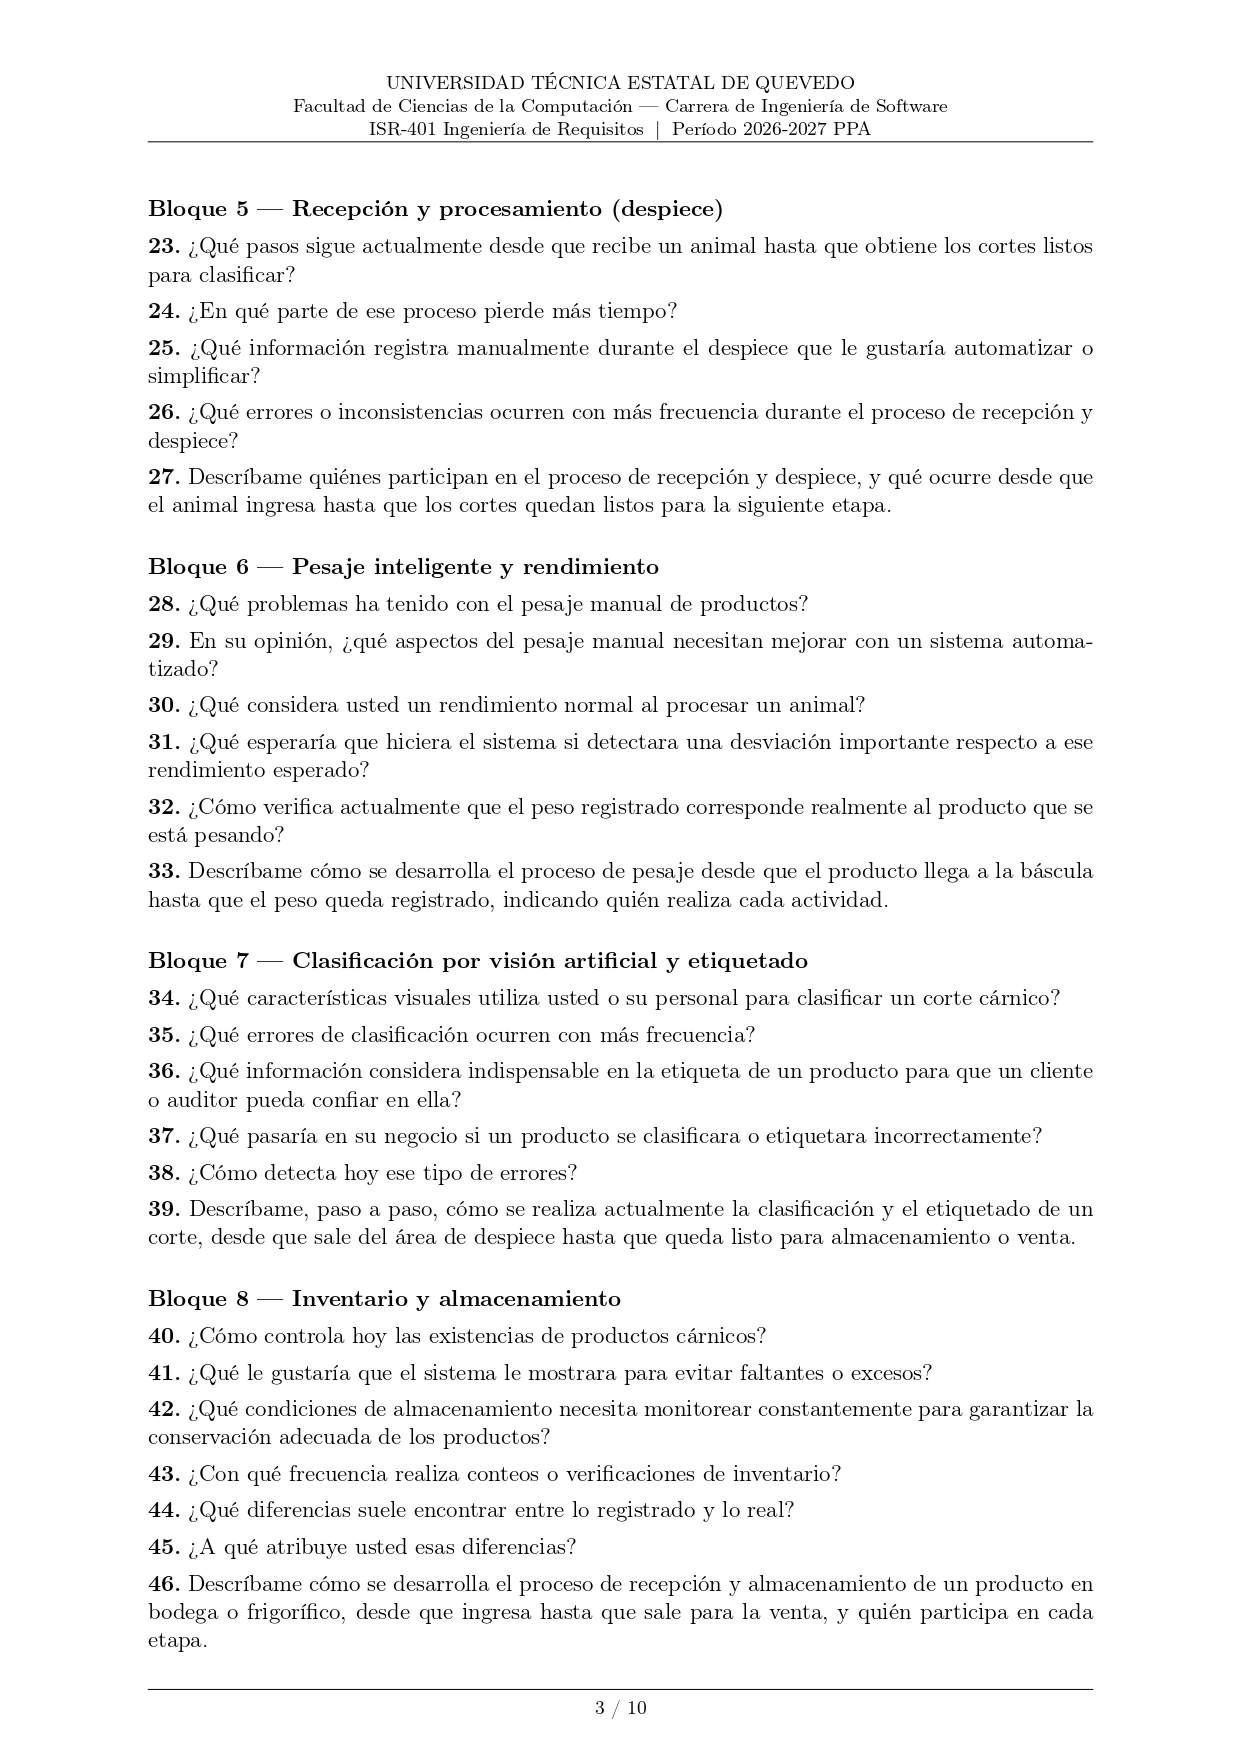
\includegraphics[width=\textwidth,keepaspectratio]{figures/A02_Instrumentos_Recoleccion_page-0003.jpg}
    \label{fig:diagrama_clases}
\end{figure}

\begin{figure}[H]
    \centering
    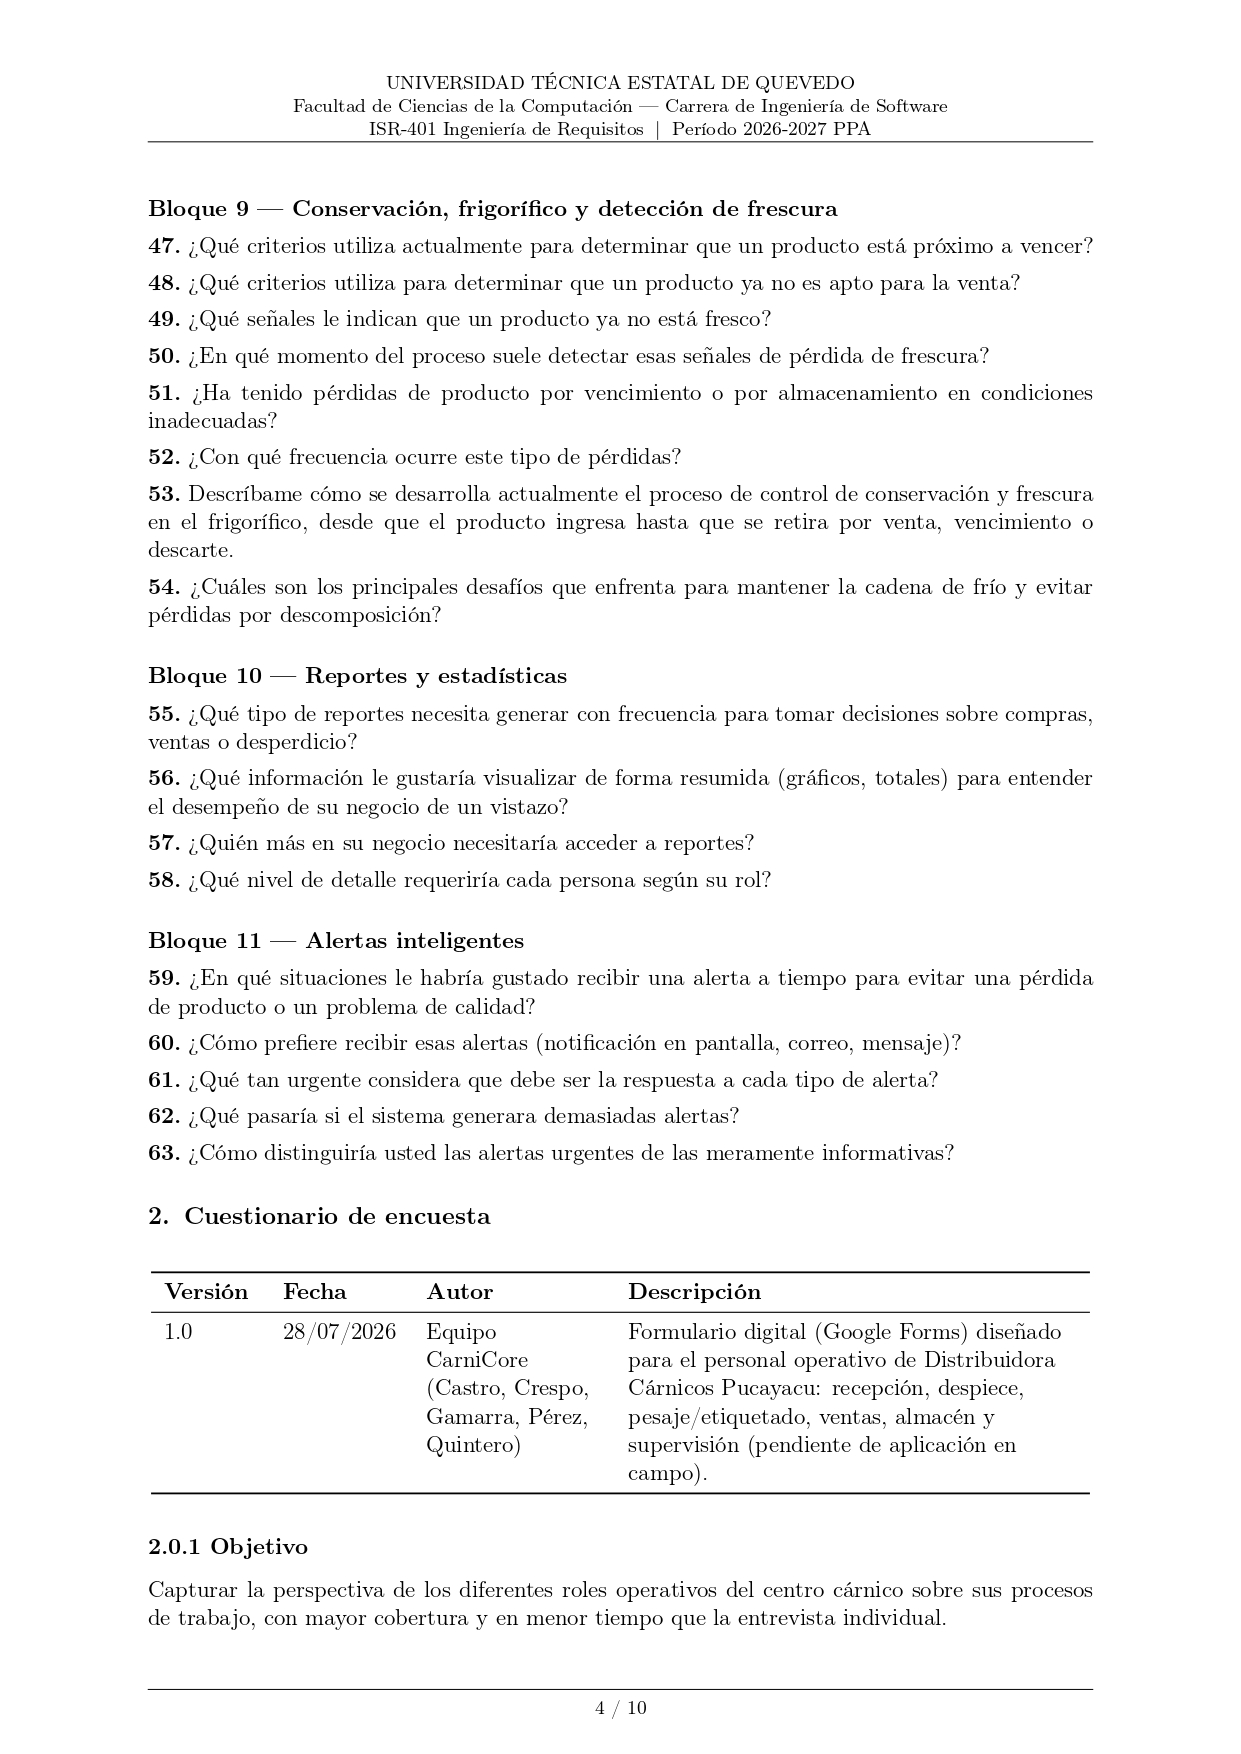
\includegraphics[width=\textwidth,keepaspectratio]{figures/A02_Instrumentos_Recoleccion_page-0004.jpg}
    \label{fig:diagrama_clases}
\end{figure}

\begin{figure}[H]
    \centering
    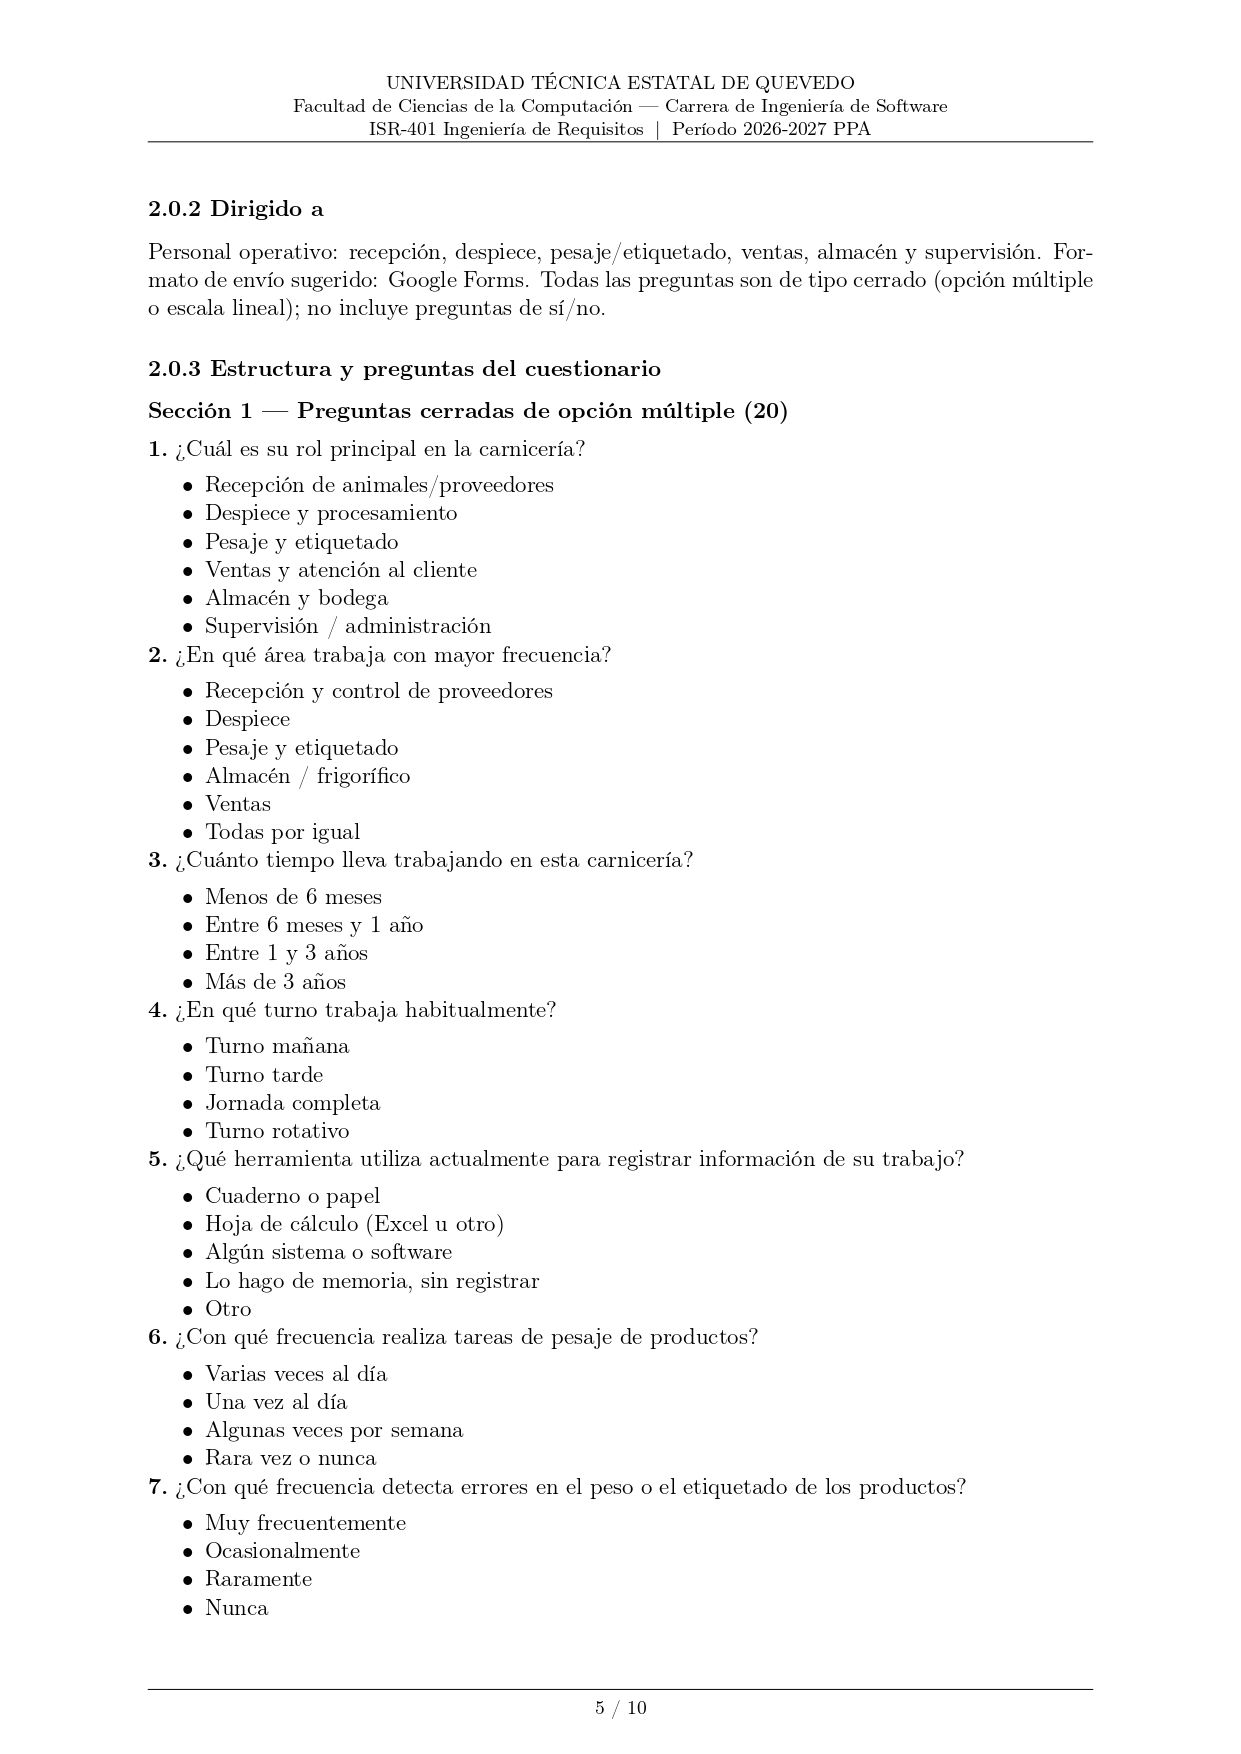
\includegraphics[width=\textwidth,keepaspectratio]{figures/A02_Instrumentos_Recoleccion_page-0005.jpg}
    \label{fig:diagrama_clases}
\end{figure}



\subsection{Consentimientos Informados}
\begin{figure}[H]
    \centering
    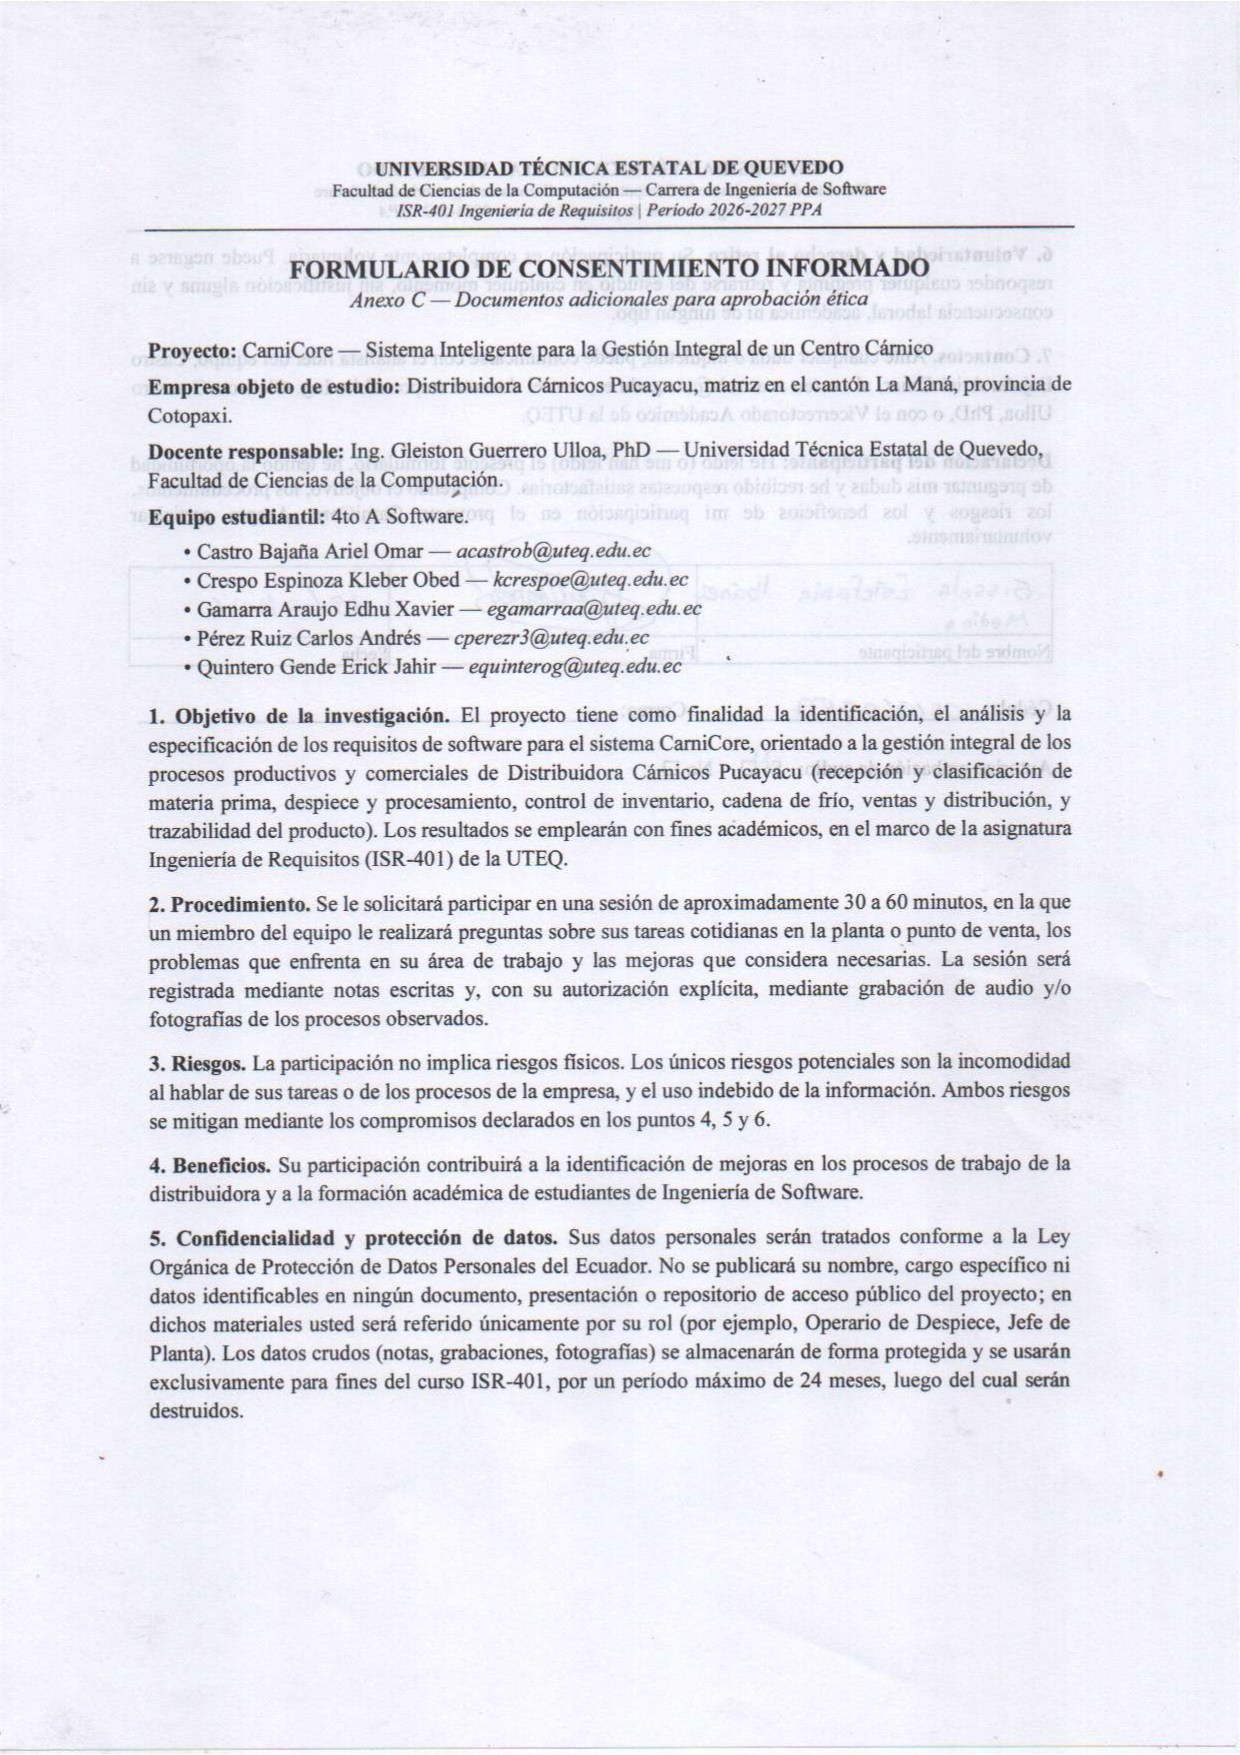
\includegraphics[width=\textwidth,keepaspectratio]{figures/2026-07-28_Propietaria_ENTR-05_Consentimiento_page-0001.jpg}
    \label{fig:diagrama_clases}
\end{figure}

\begin{figure}[H]
    \centering
    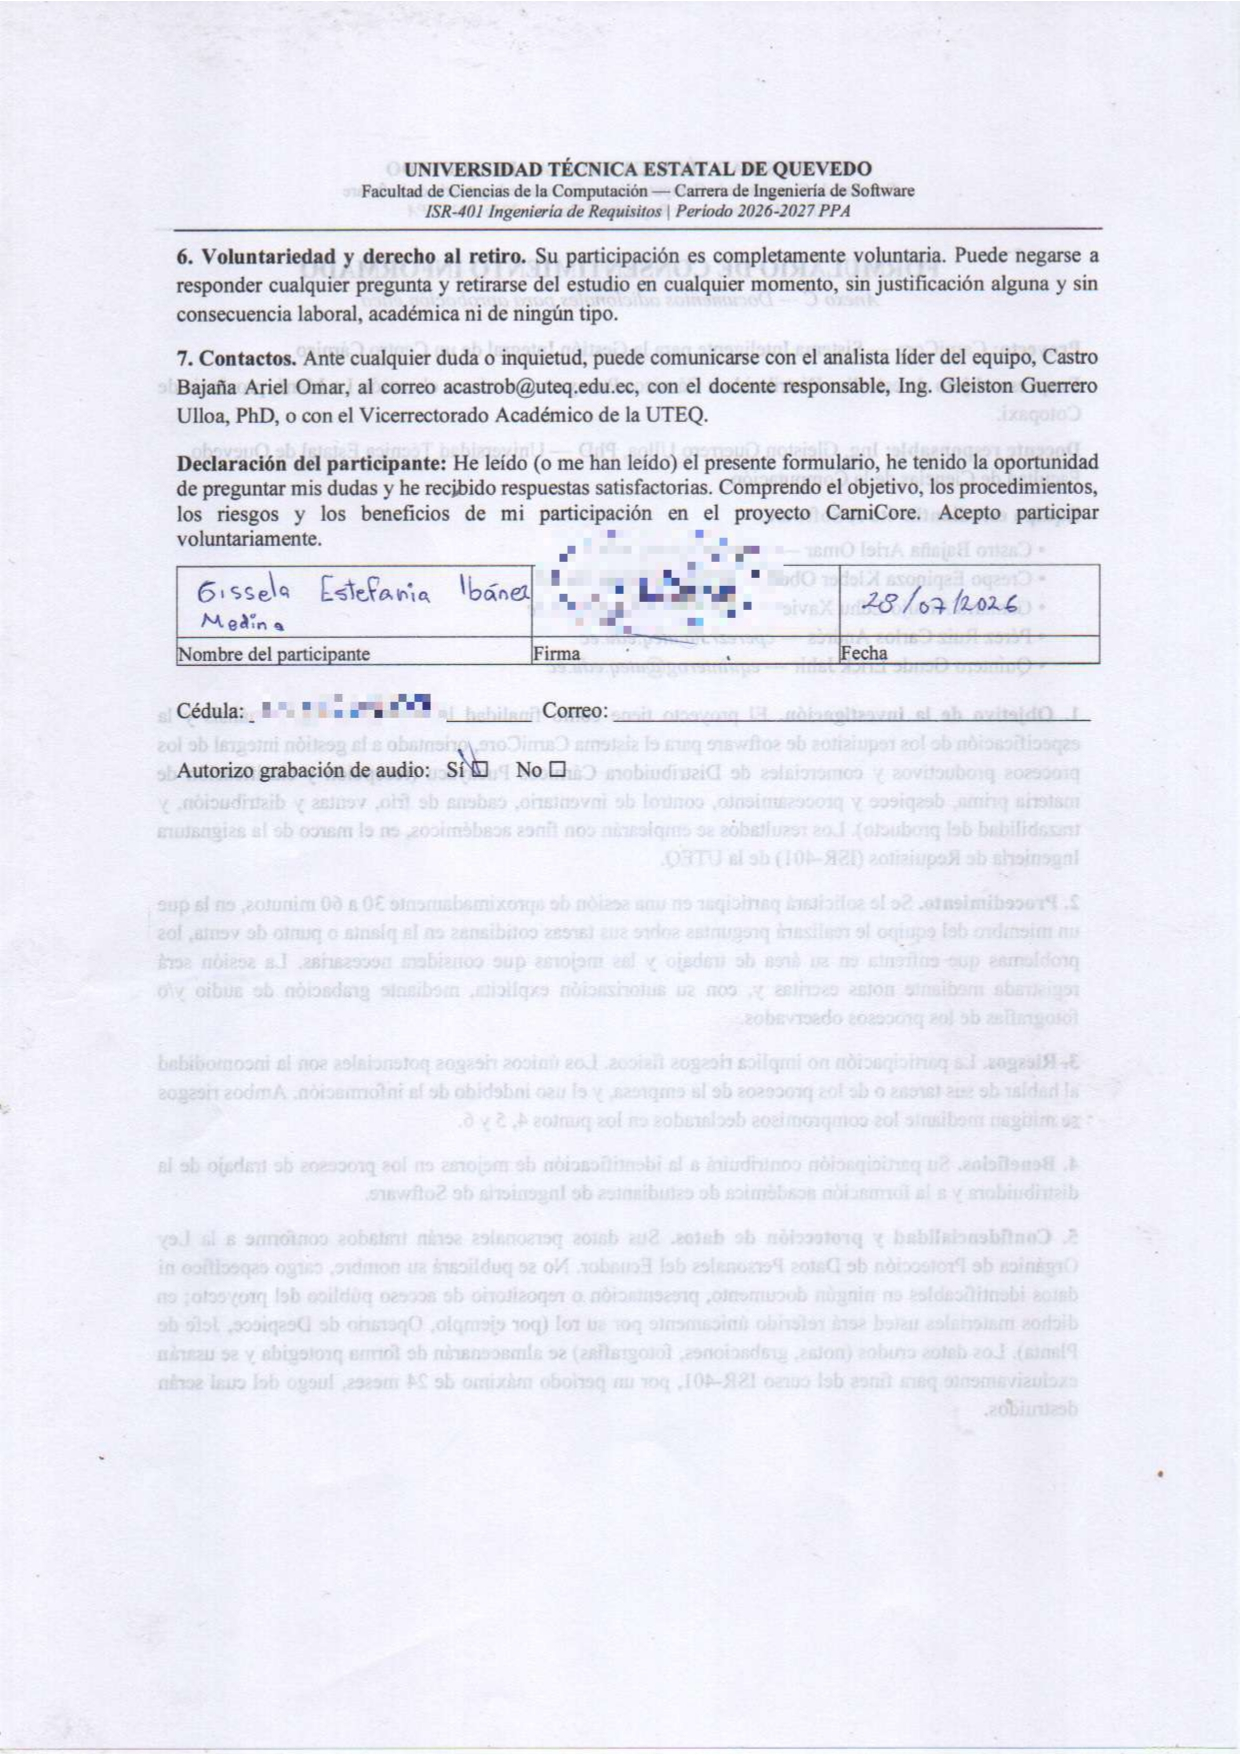
\includegraphics[width=\textwidth,keepaspectratio]{figures/2026-07-28_Propietaria_ENTR-05_Consentimiento_page-0002.jpg}
    \label{fig:diagrama_clases}
\end{figure}

\begin{figure}[H]
    \centering
    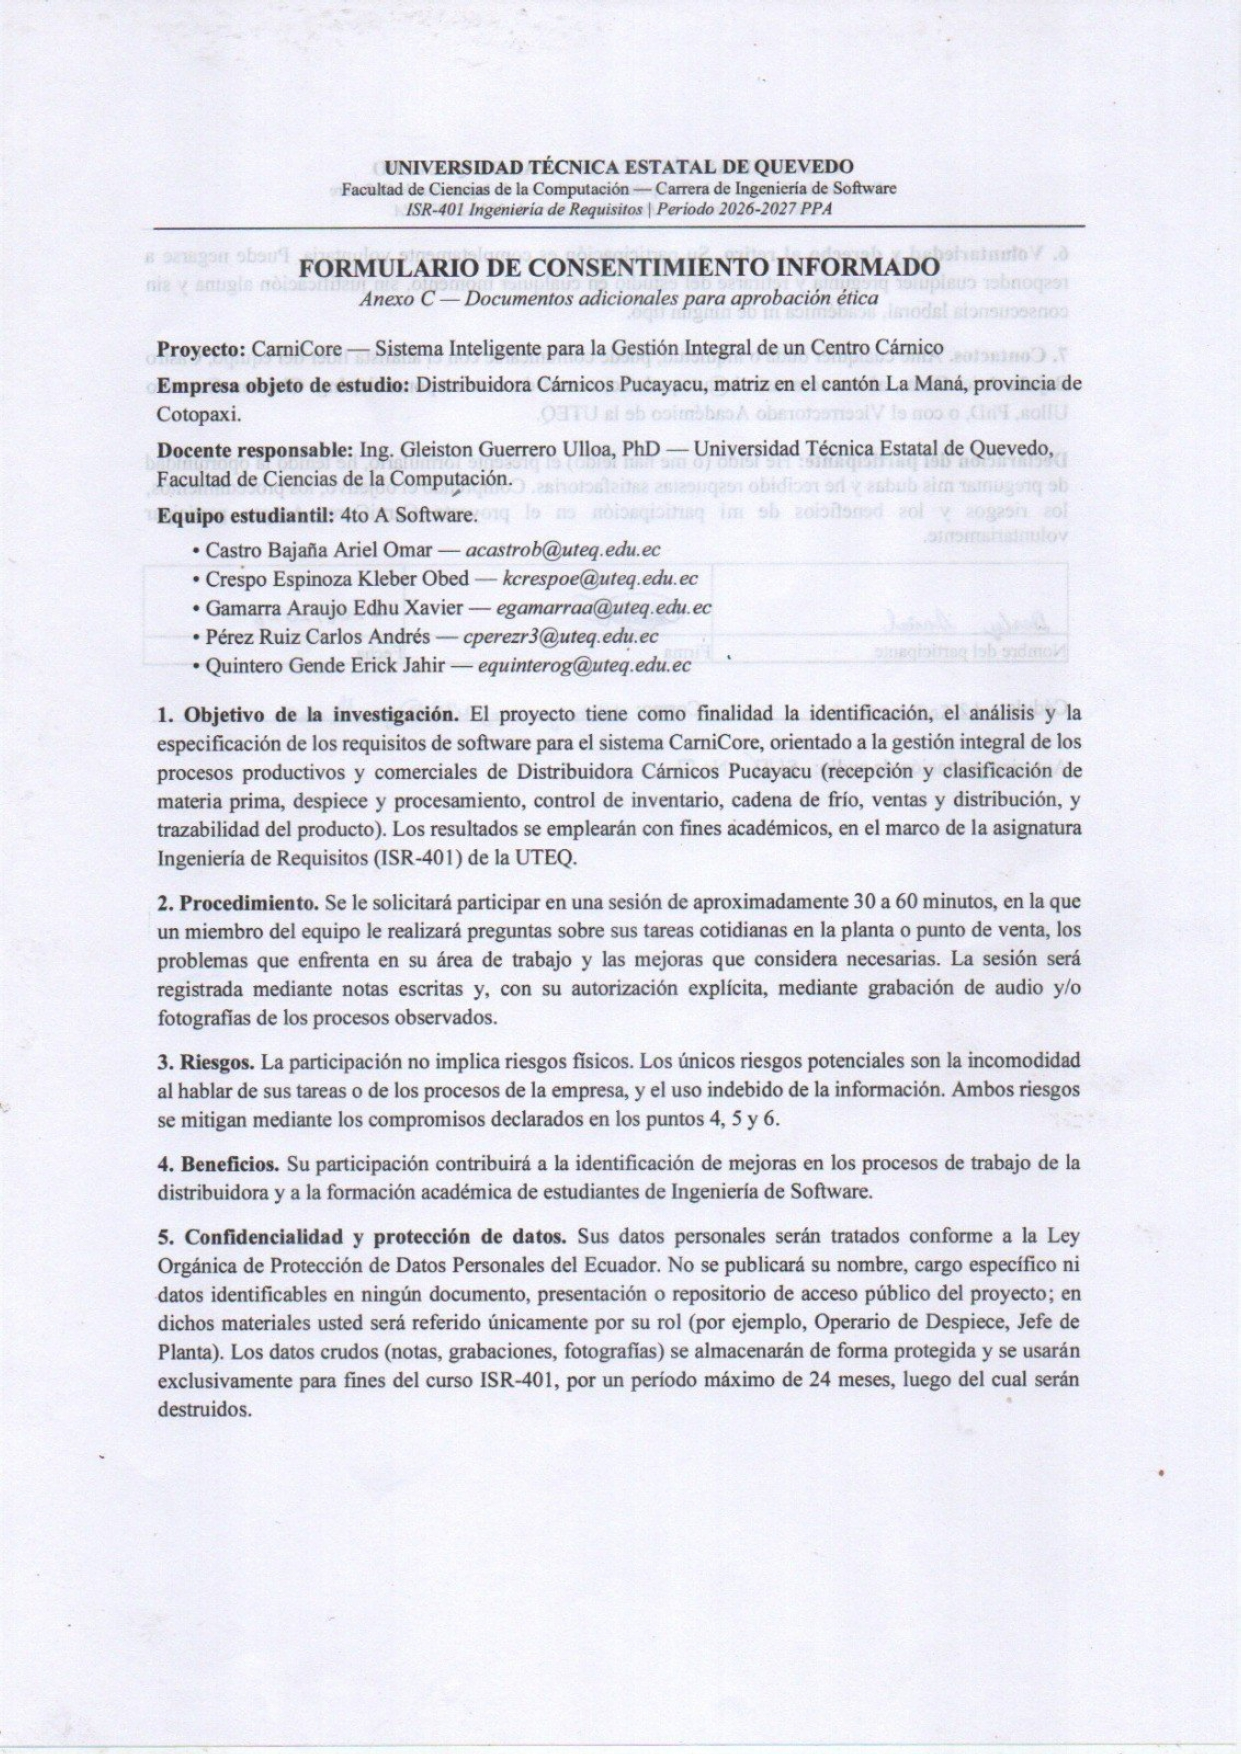
\includegraphics[width=\textwidth,keepaspectratio]{figures/2026-08-01_AdministradorDeBodega_ENTR-01_Consentimiento_page-0001.jpg}
    \label{fig:diagrama_clases}
\end{figure}

\begin{figure}[H]
    \centering
    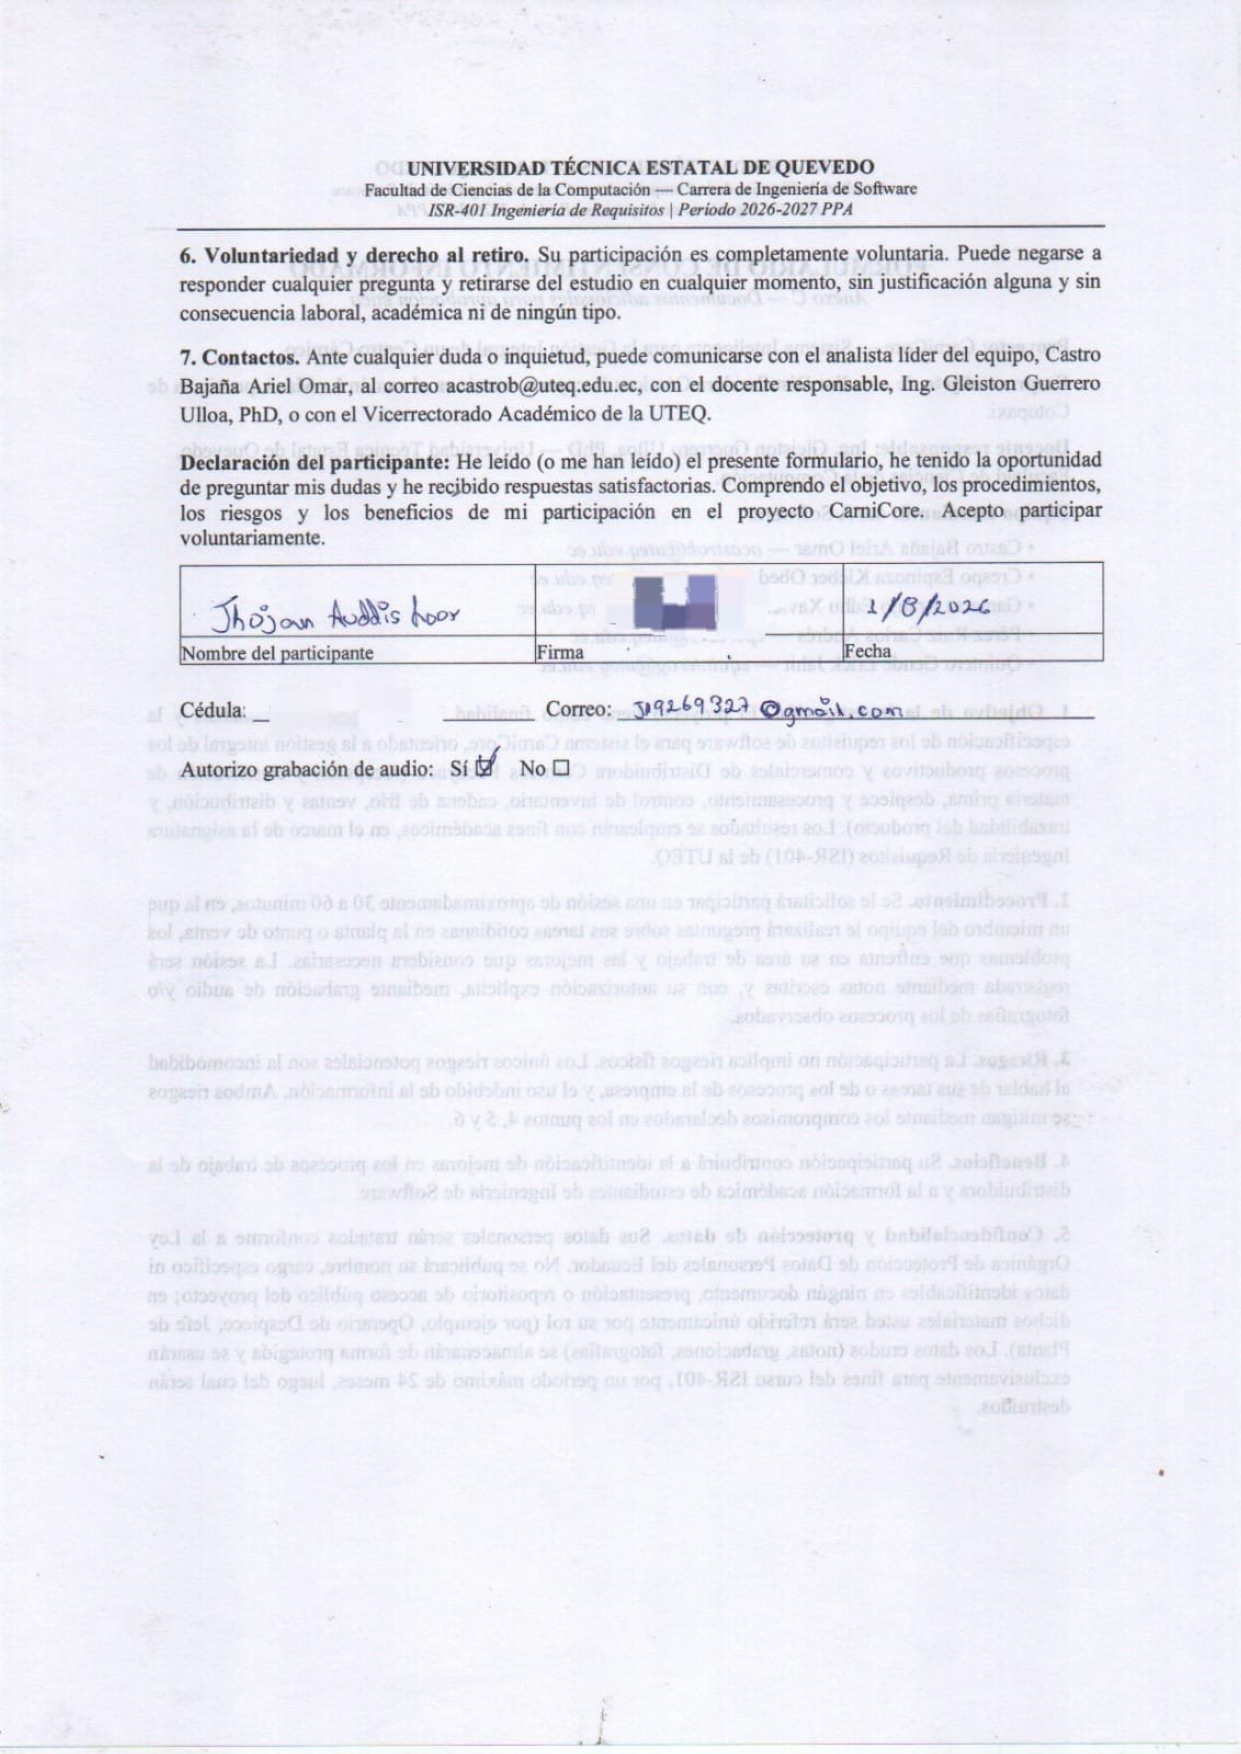
\includegraphics[width=\textwidth,keepaspectratio]{figures/2026-08-01_AdministradorDeBodega_ENTR-01_Consentimiento_page-0002.jpg}
    \label{fig:diagrama_clases}
\end{figure}

\begin{figure}[H]
    \centering
    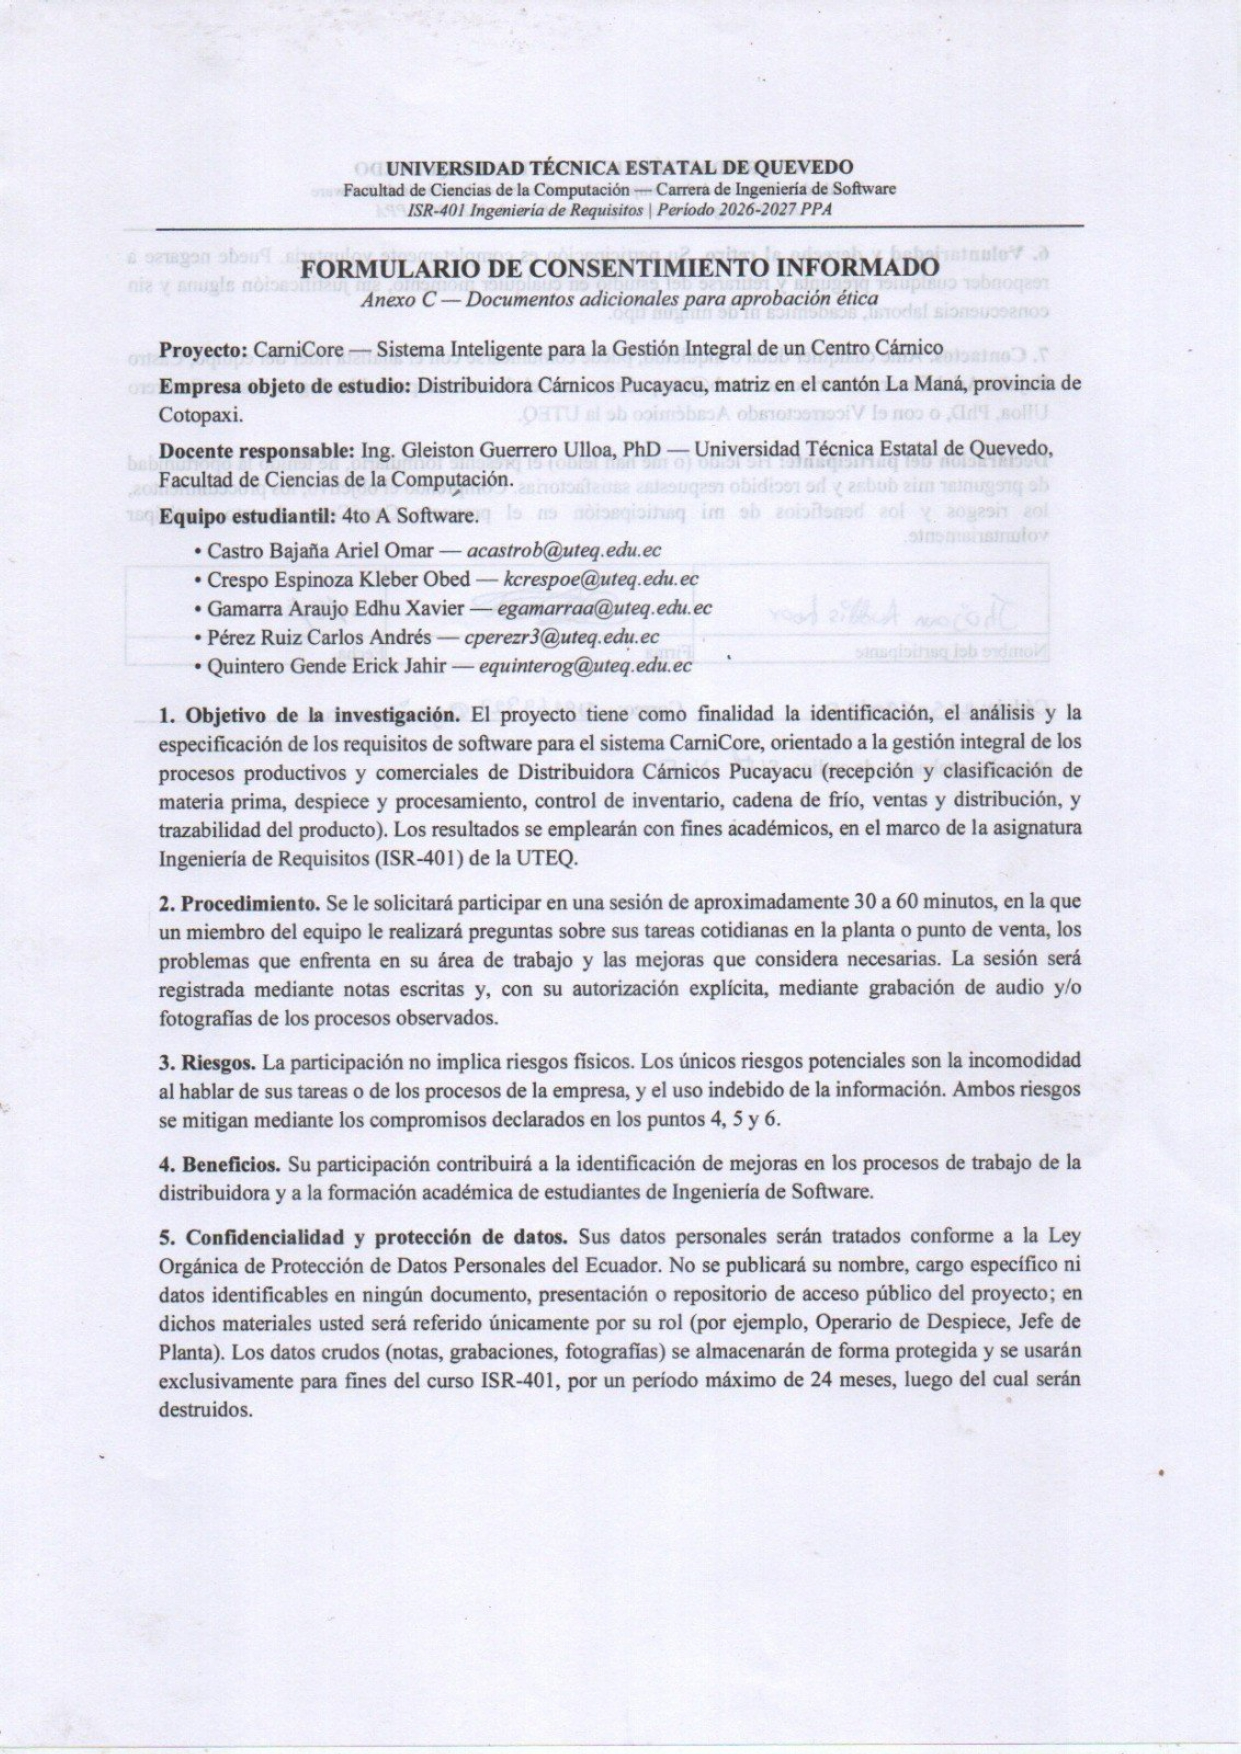
\includegraphics[width=\textwidth,keepaspectratio]{figures/AdminBodega1.jpg}
    \label{fig:diagrama_clases}
\end{figure}

\begin{figure}[H]
    \centering
    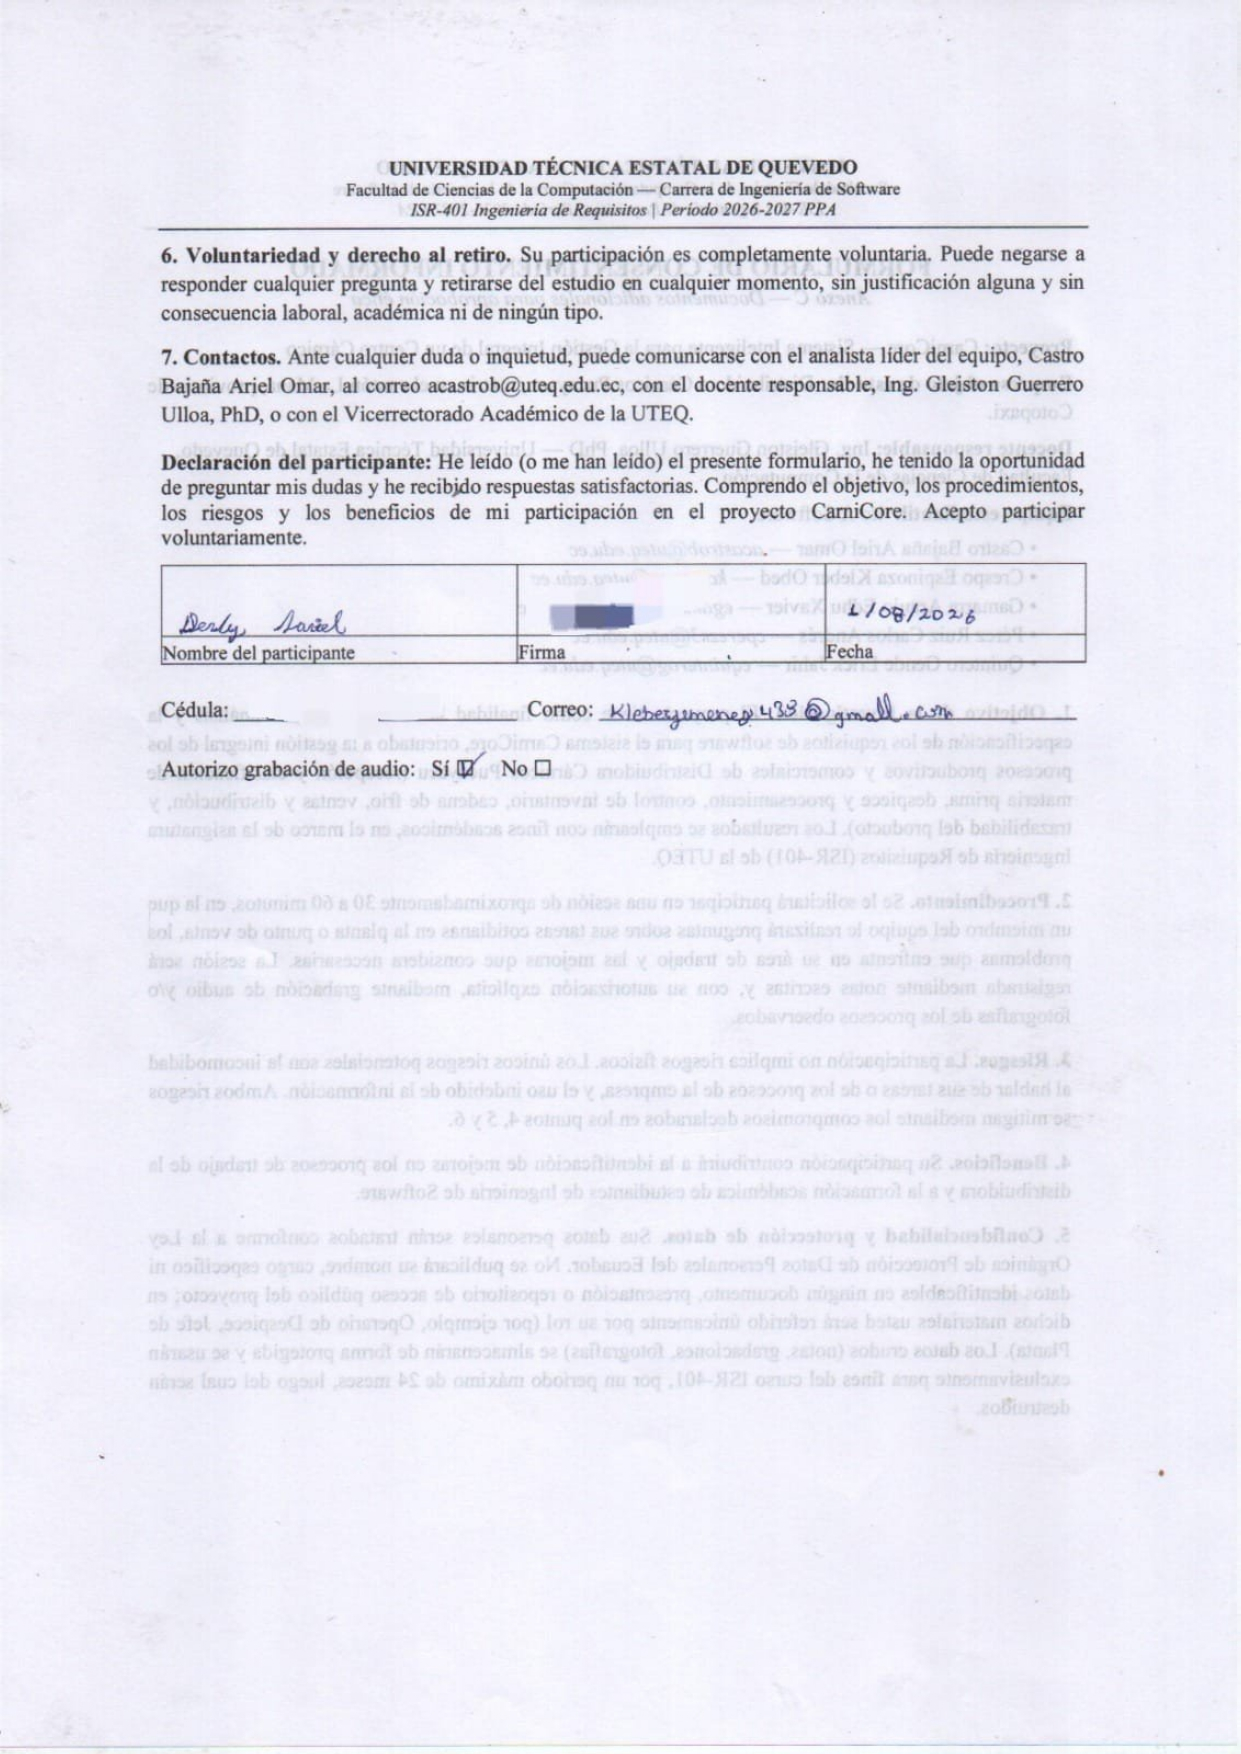
\includegraphics[width=\textwidth,keepaspectratio]{figures/AdminBodega2.jpg}
    \label{fig:diagrama_clases}
\end{figure}

\begin{figure}[H]
    \centering
    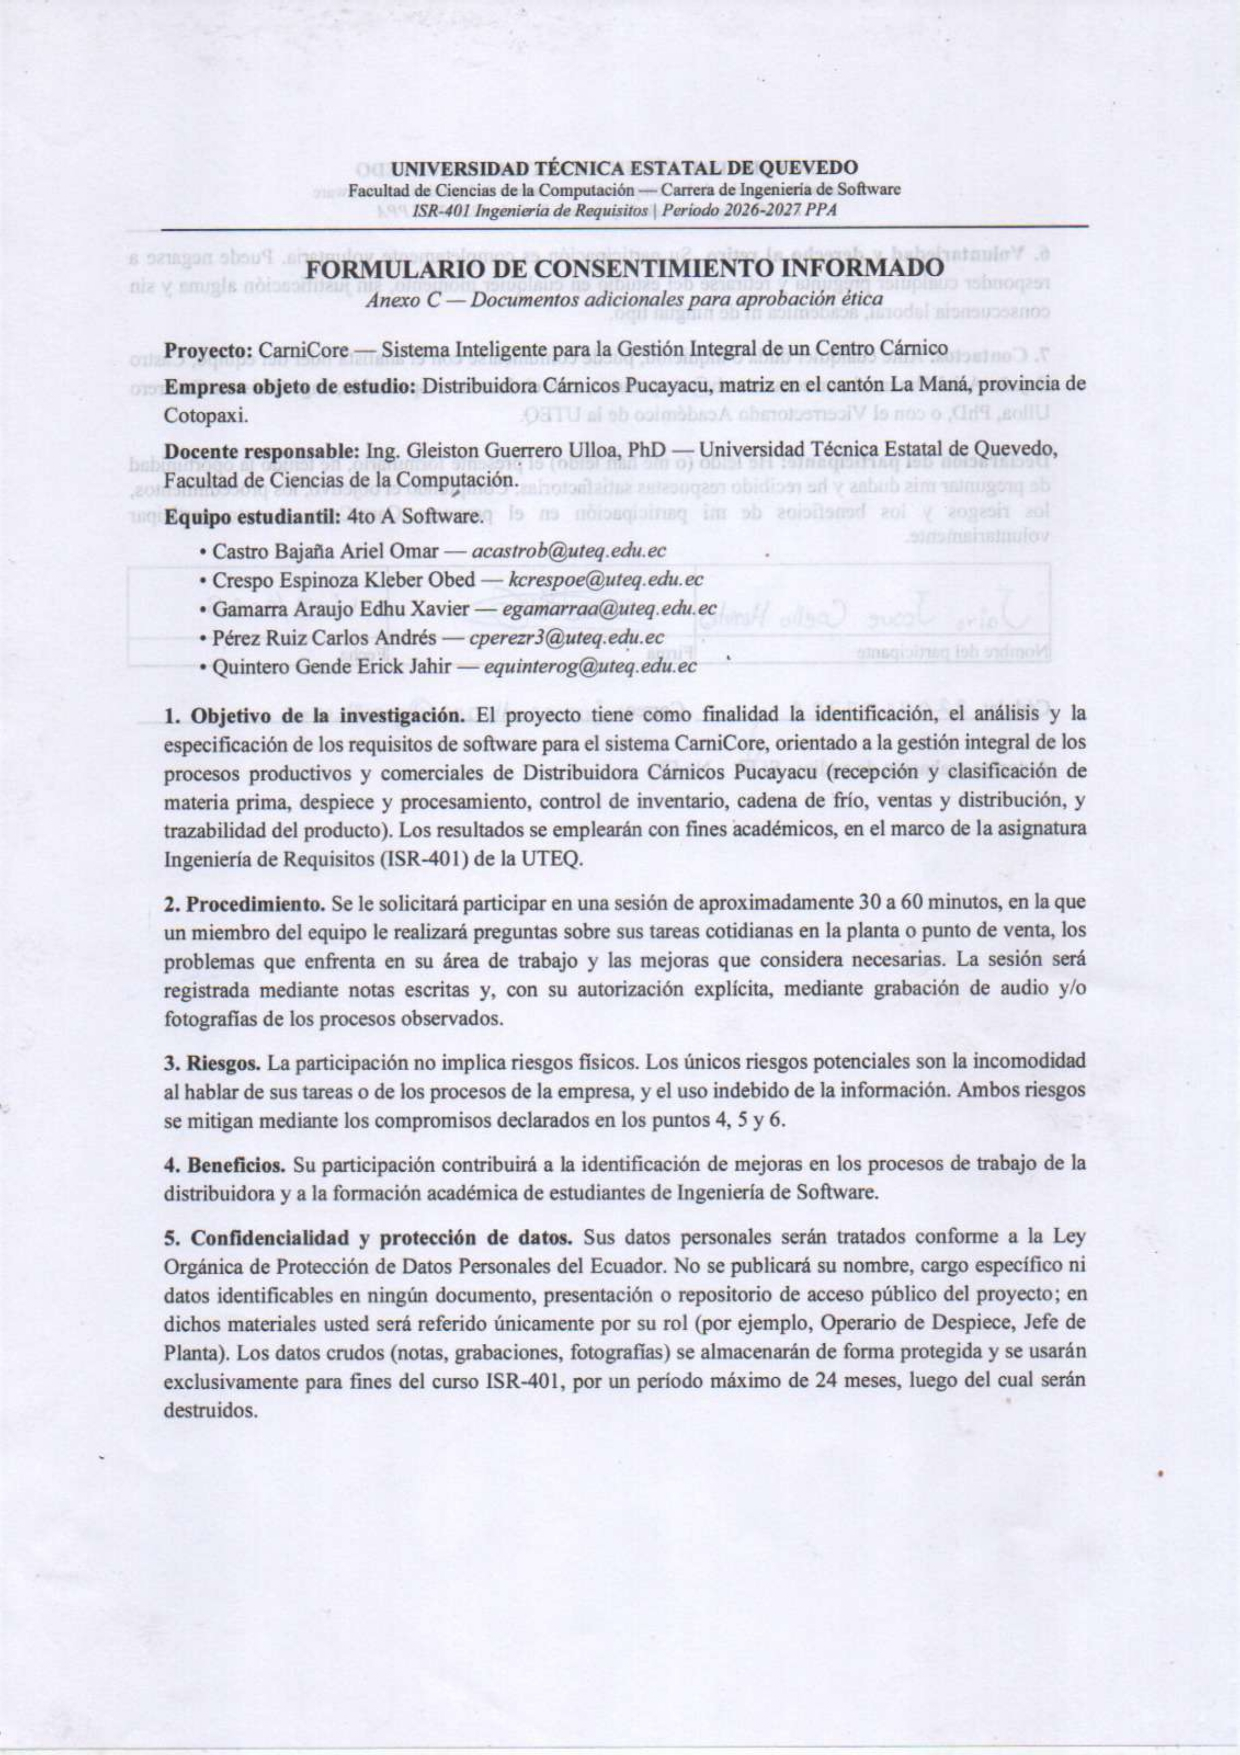
\includegraphics[width=\textwidth,keepaspectratio]{figures/2026-08-01_CarniceroPrincipal_ENTR-03_Consentimiento_page-0001.jpg}
    \label{fig:diagrama_clases}
\end{figure}

\begin{figure}[H]
    \centering
    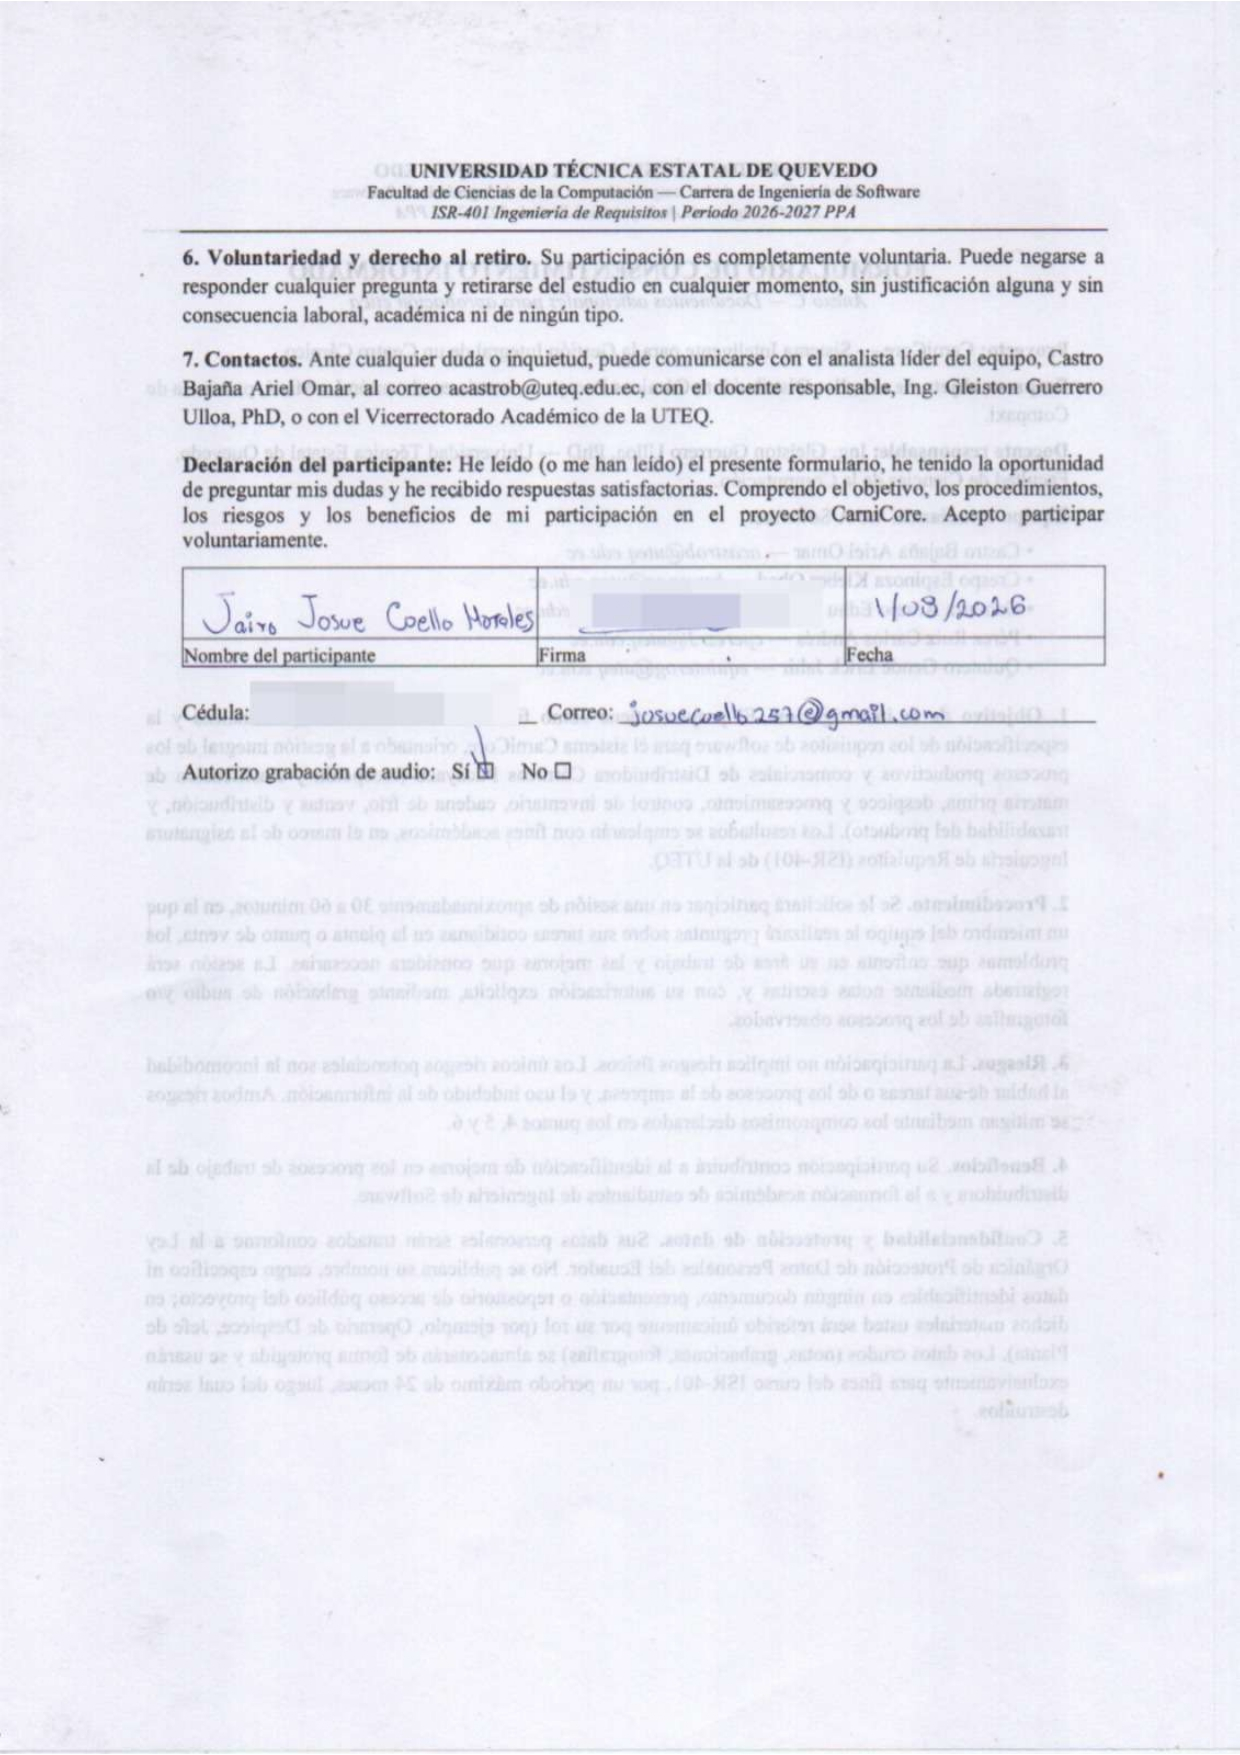
\includegraphics[width=\textwidth,keepaspectratio]{figures/2026-08-01_CarniceroPrincipal_ENTR-03_Consentimiento_page-0002.jpg}
    \label{fig:diagrama_clases}
\end{figure}

\begin{figure}[H]
    \centering
    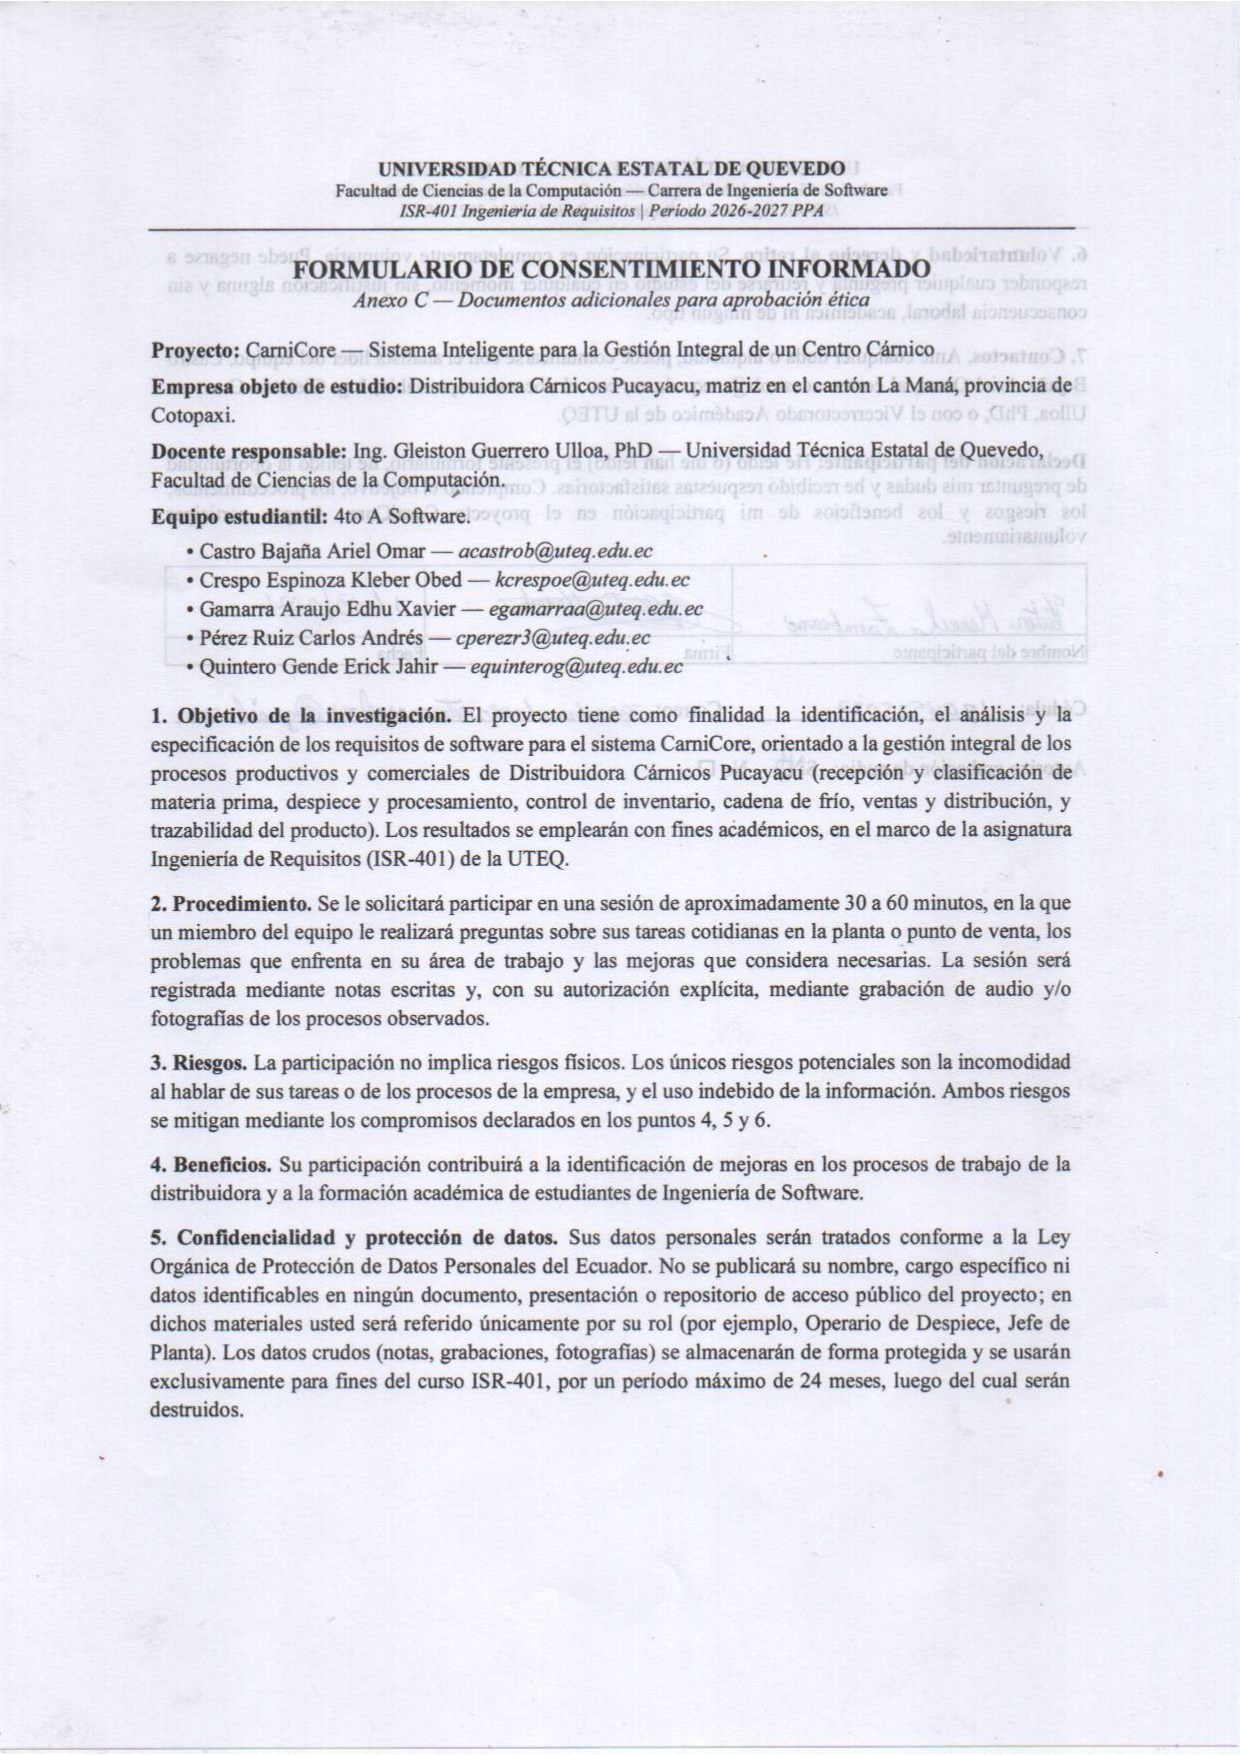
\includegraphics[width=\textwidth,keepaspectratio]{figures/2026-08-01_OperarioRecepcionPesaje_ENTR-04_Consentimiento_page-0001.jpg}
    \label{fig:diagrama_clases}
\end{figure}


\begin{figure}[H]
    \centering
    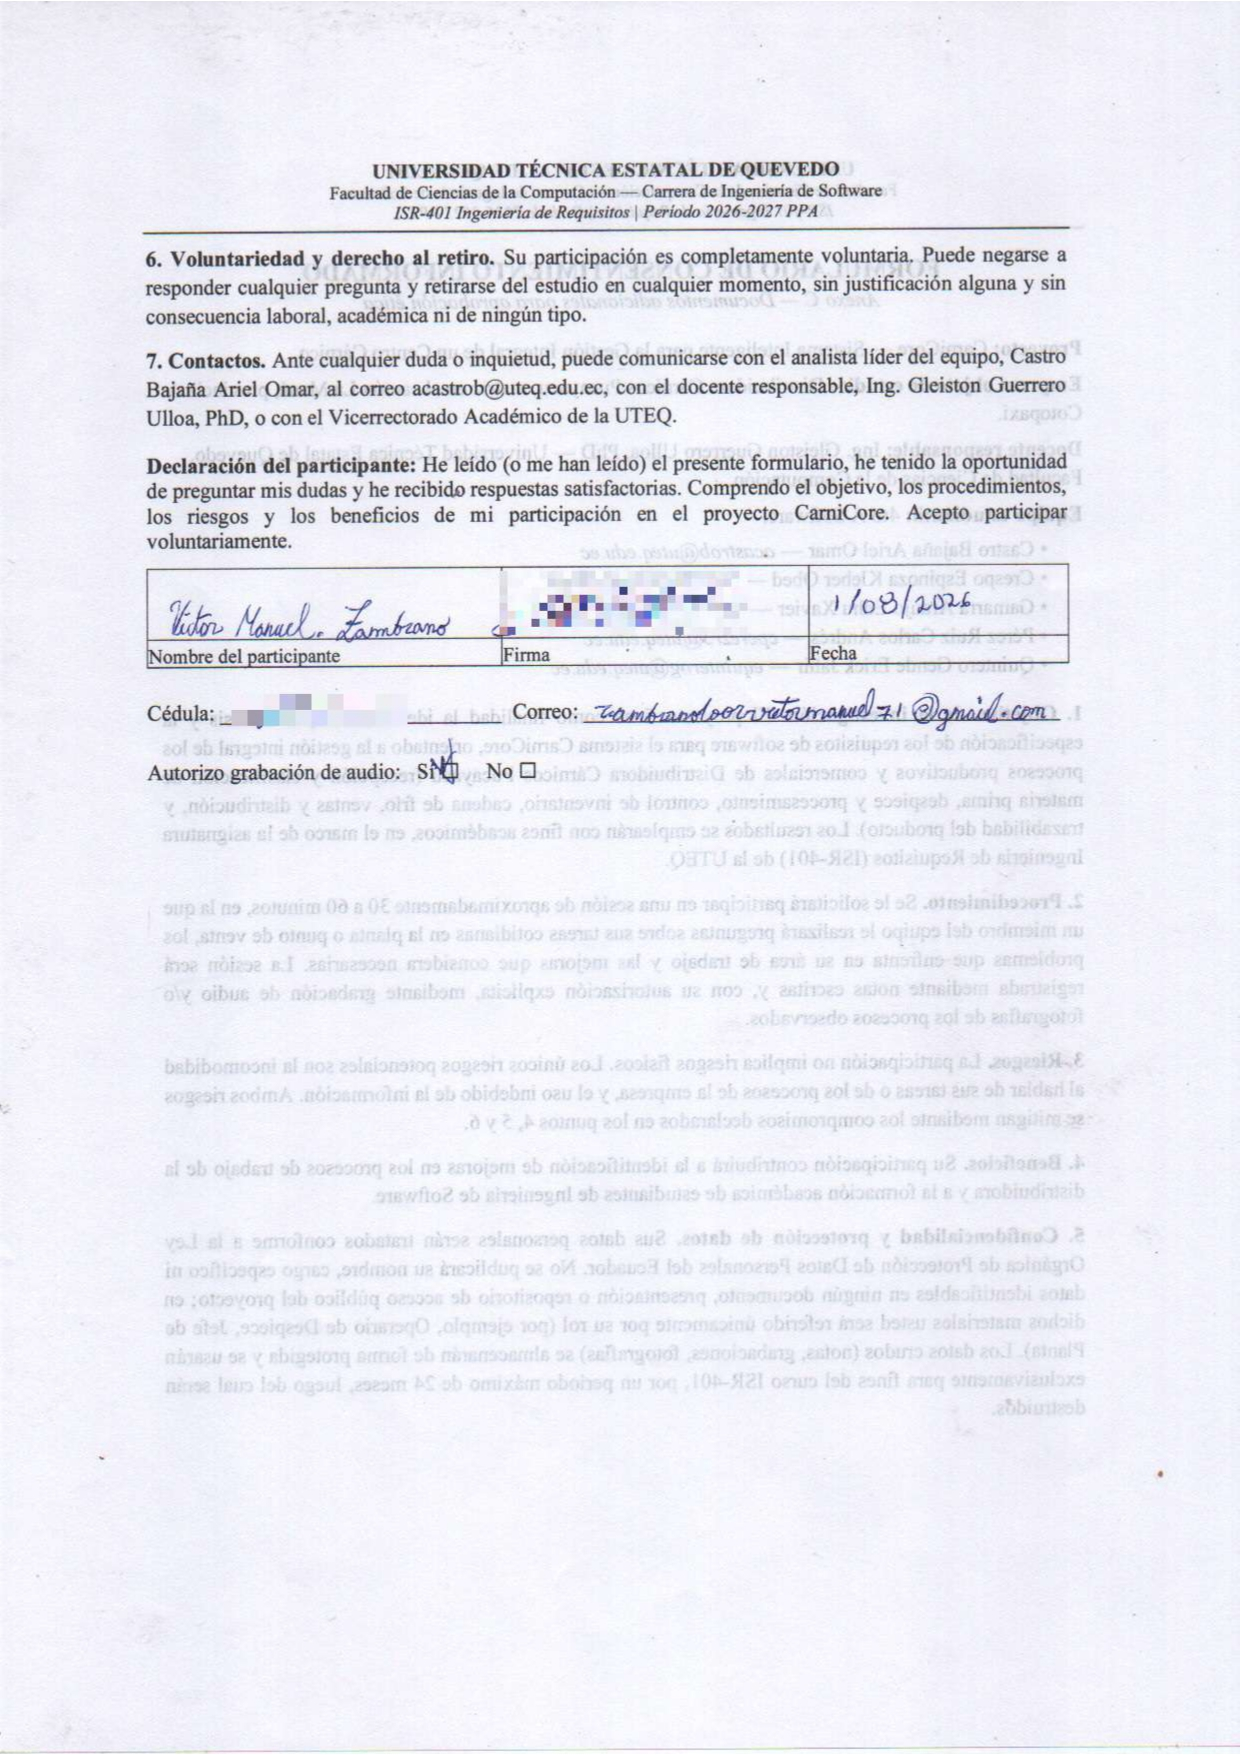
\includegraphics[width=\textwidth,keepaspectratio]{figures/2026-08-01_OperarioRecepcionPesaje_ENTR-04_Consentimiento_page-0002.jpg}
    \label{fig:diagrama_clases}
\end{figure}



\subsection{Actas de Entrevista}

\begin{figure}[H]
    \centering
    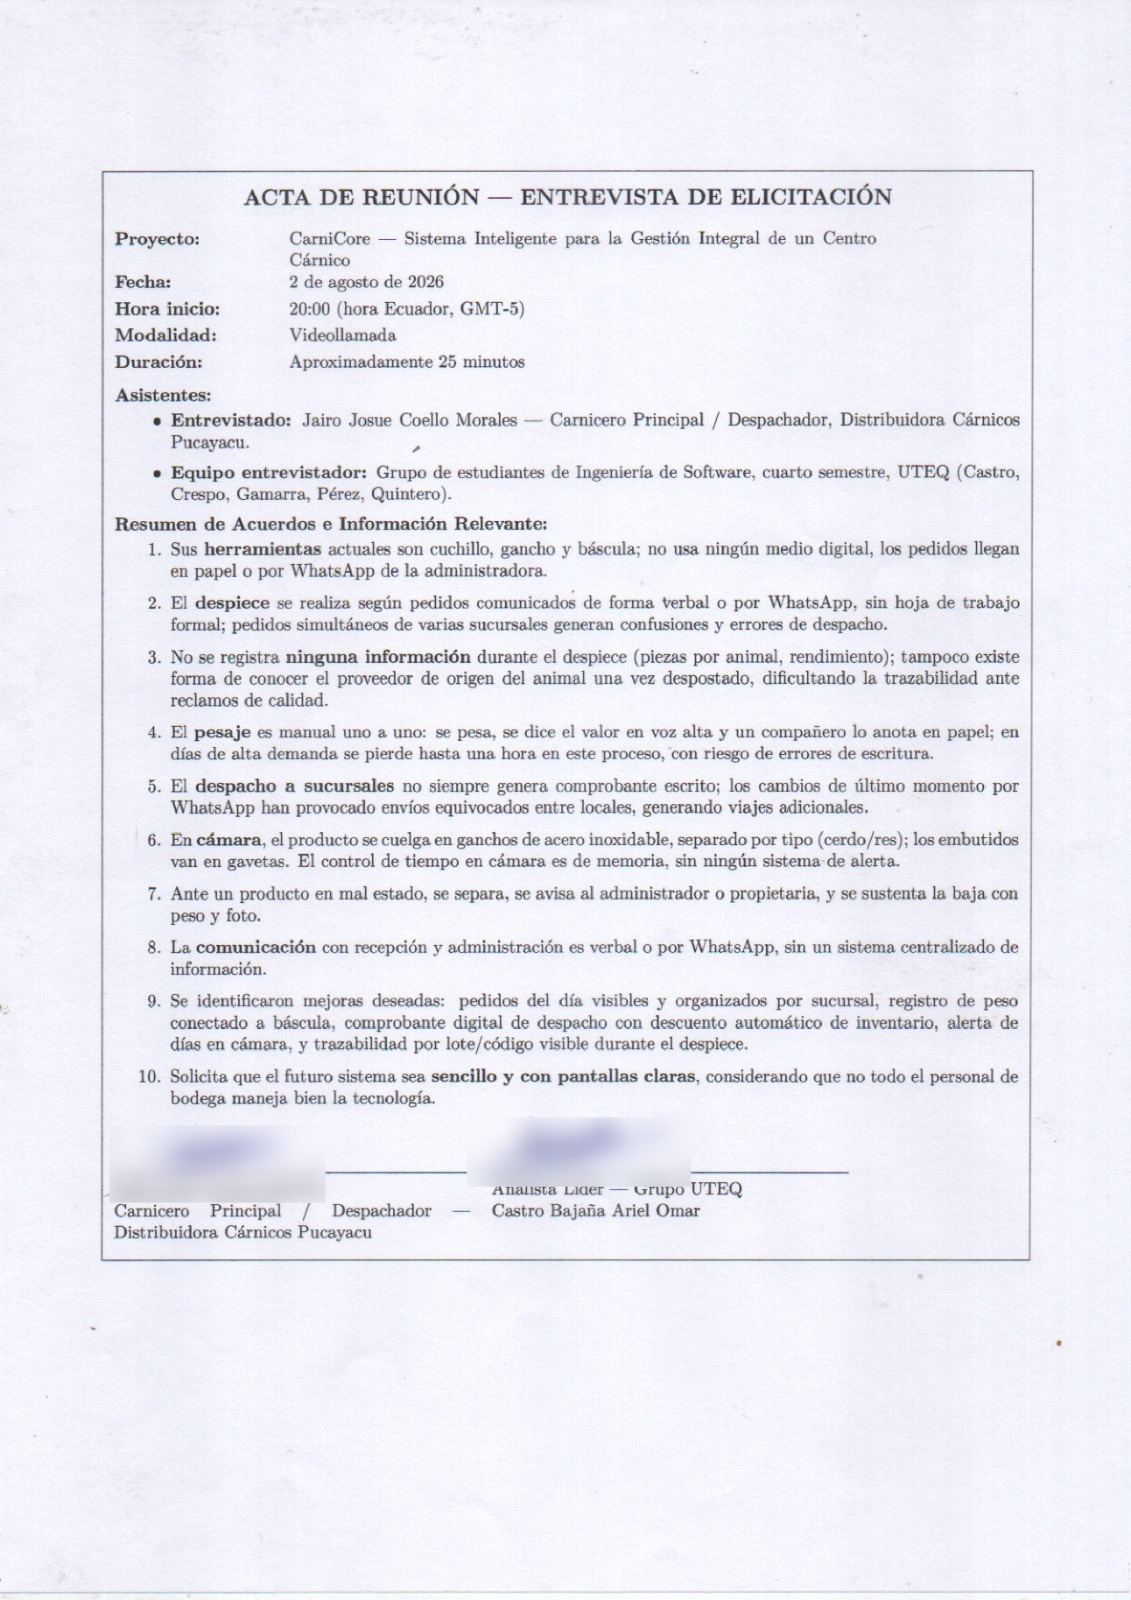
\includegraphics[width=\textwidth,keepaspectratio]{figures/ACTA-01.jpg.jpg}
    \label{fig:diagrama_clases}
\end{figure}

\begin{figure}[H]
    \centering
    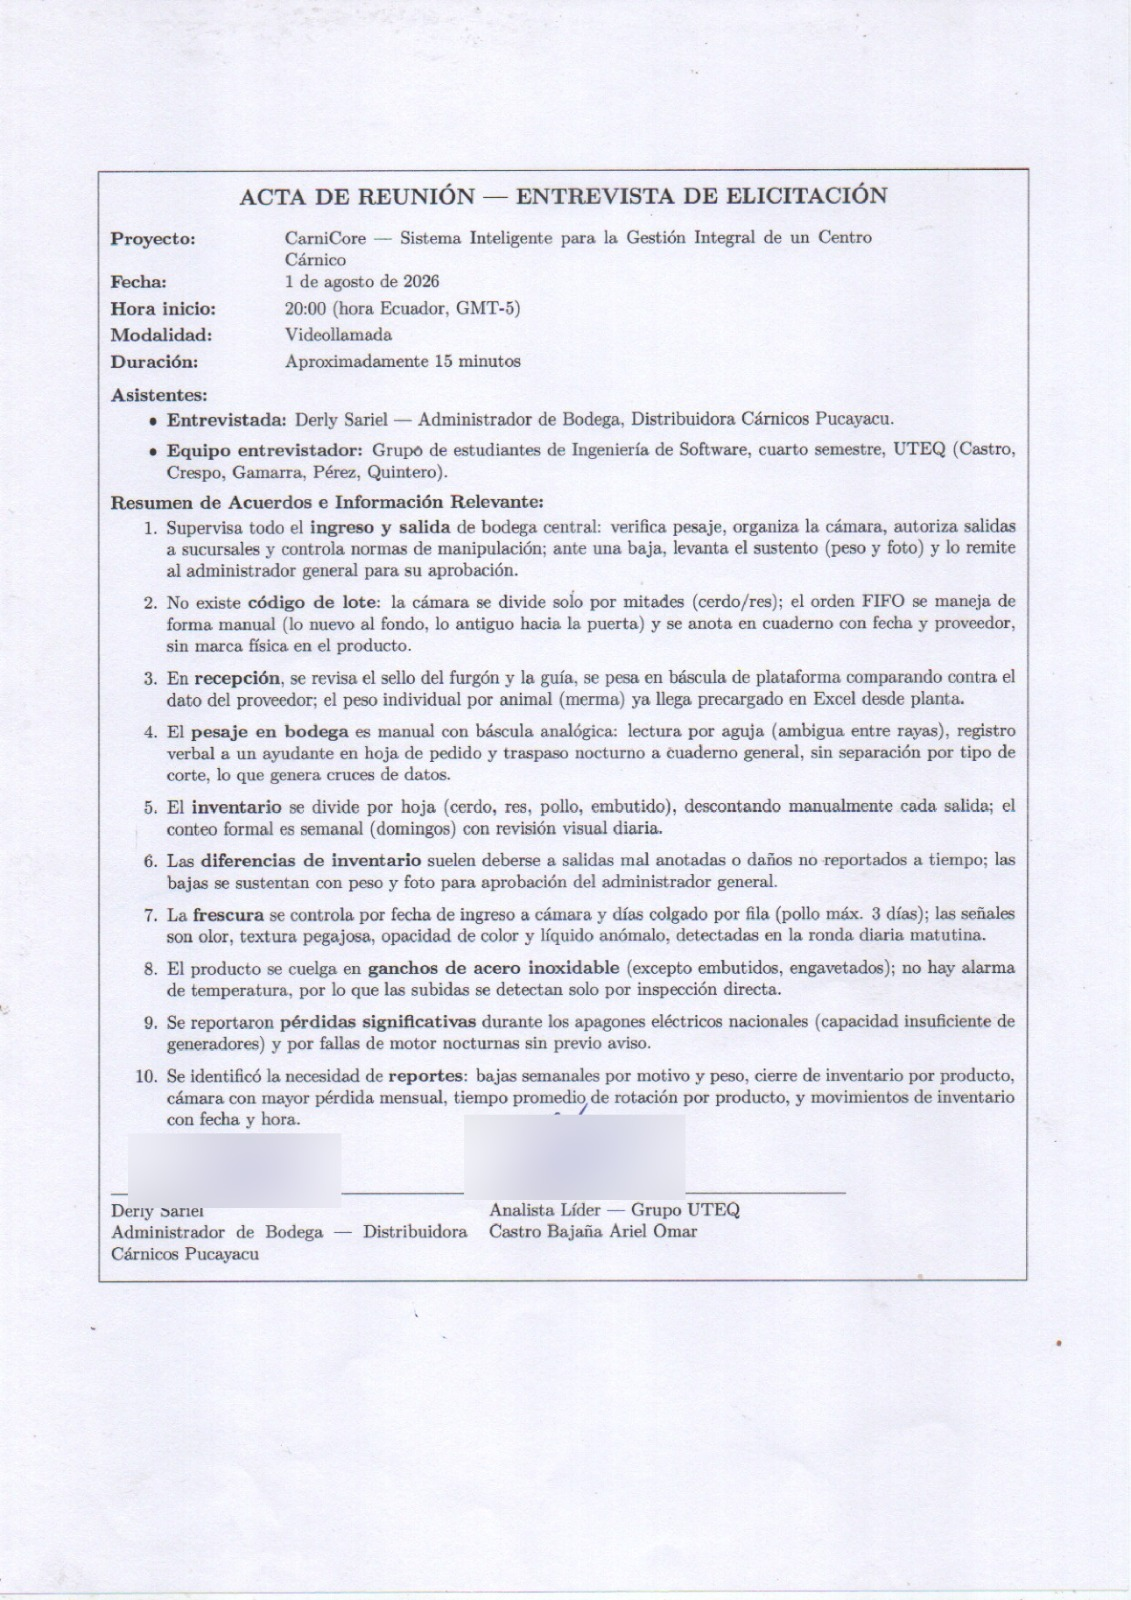
\includegraphics[width=\textwidth,keepaspectratio]{figures/ACTA-02.jpg}
    \label{fig:diagrama_clases}
\end{figure}

\begin{figure}[H]
    \centering
    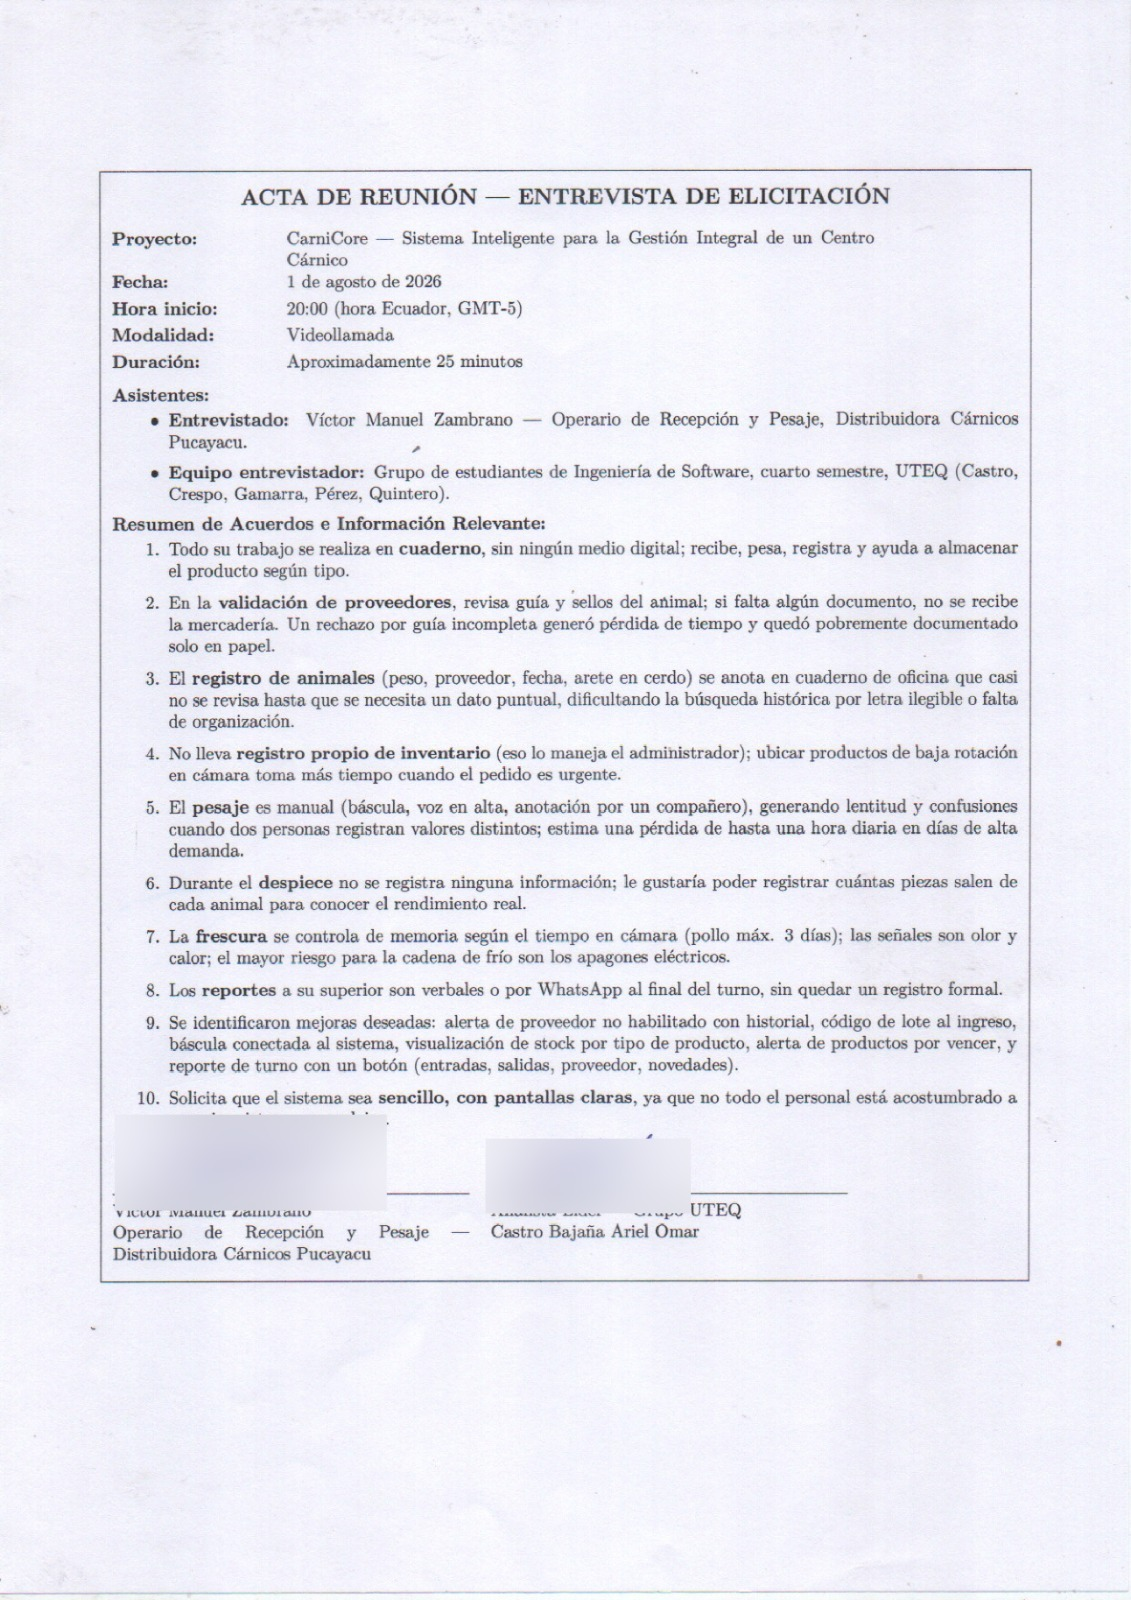
\includegraphics[width=\textwidth,keepaspectratio]{figures/ACTA-03.jpg}
    \label{fig:diagrama_clases}
\end{figure}

\begin{figure}[H]
    \centering
    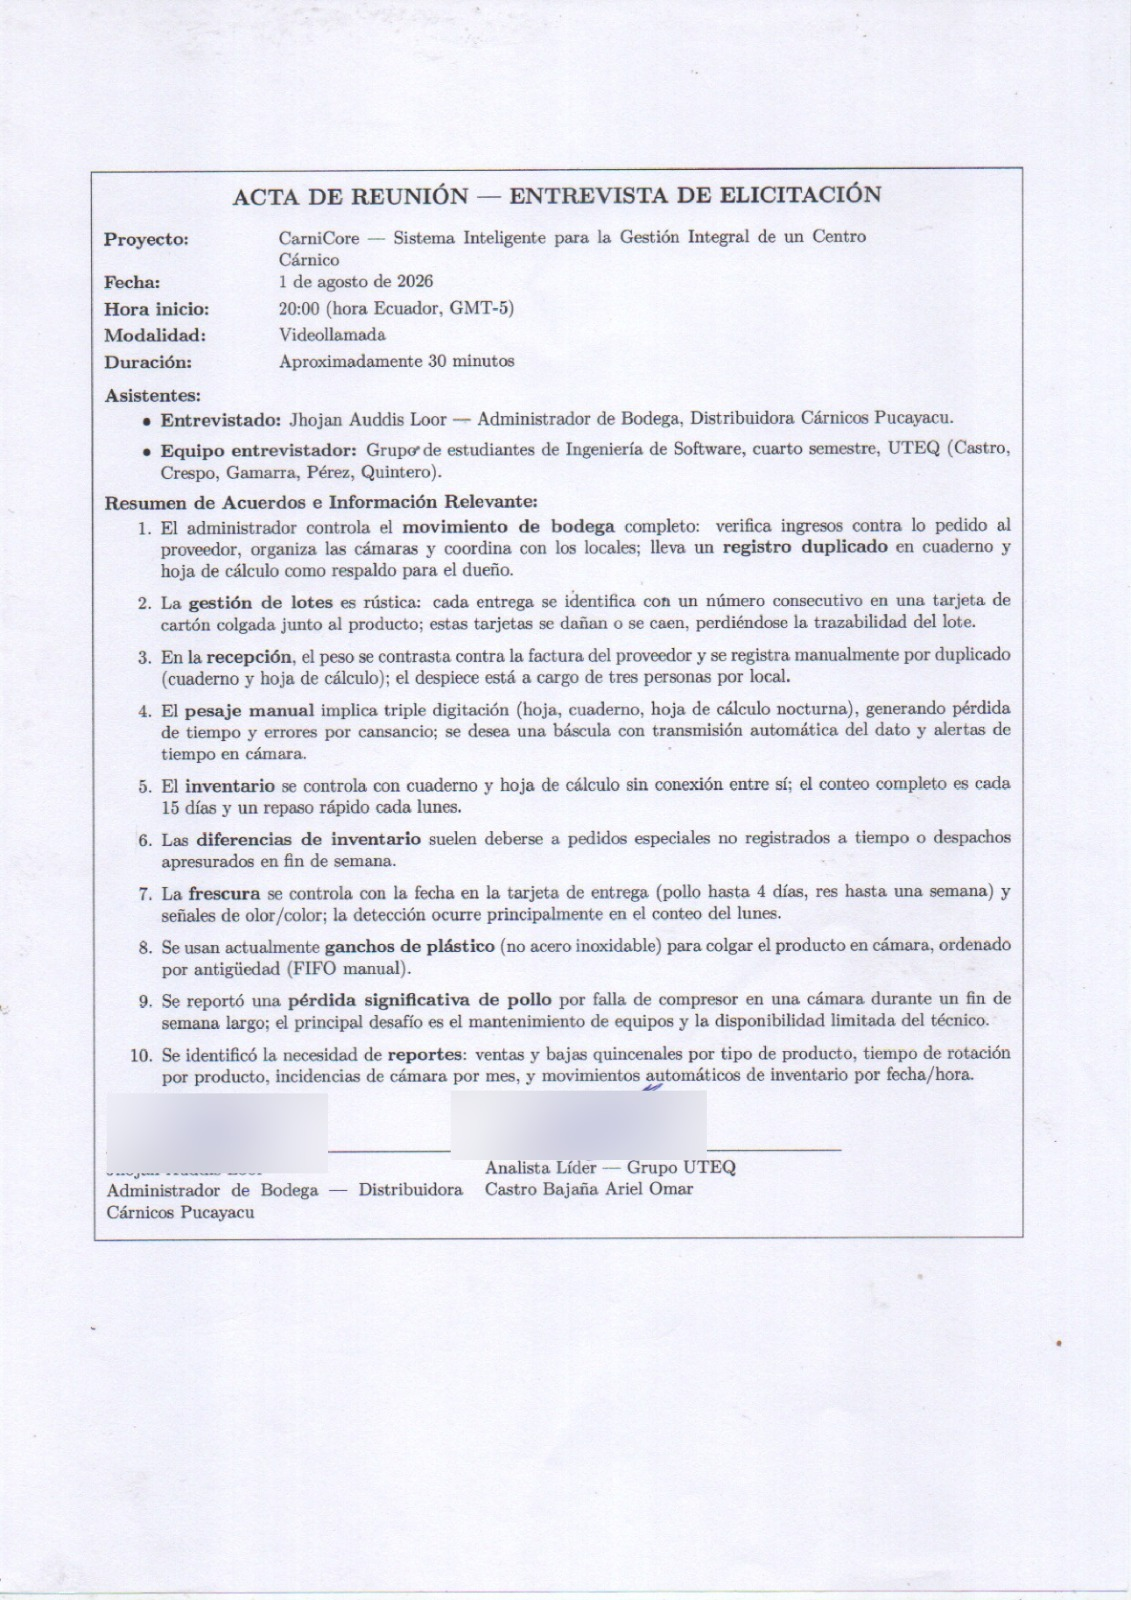
\includegraphics[width=\textwidth,keepaspectratio]{figures/ACTA-04.jpg}
    \label{fig:diagrama_clases}
\end{figure}

\begin{figure}[H]
    \centering
    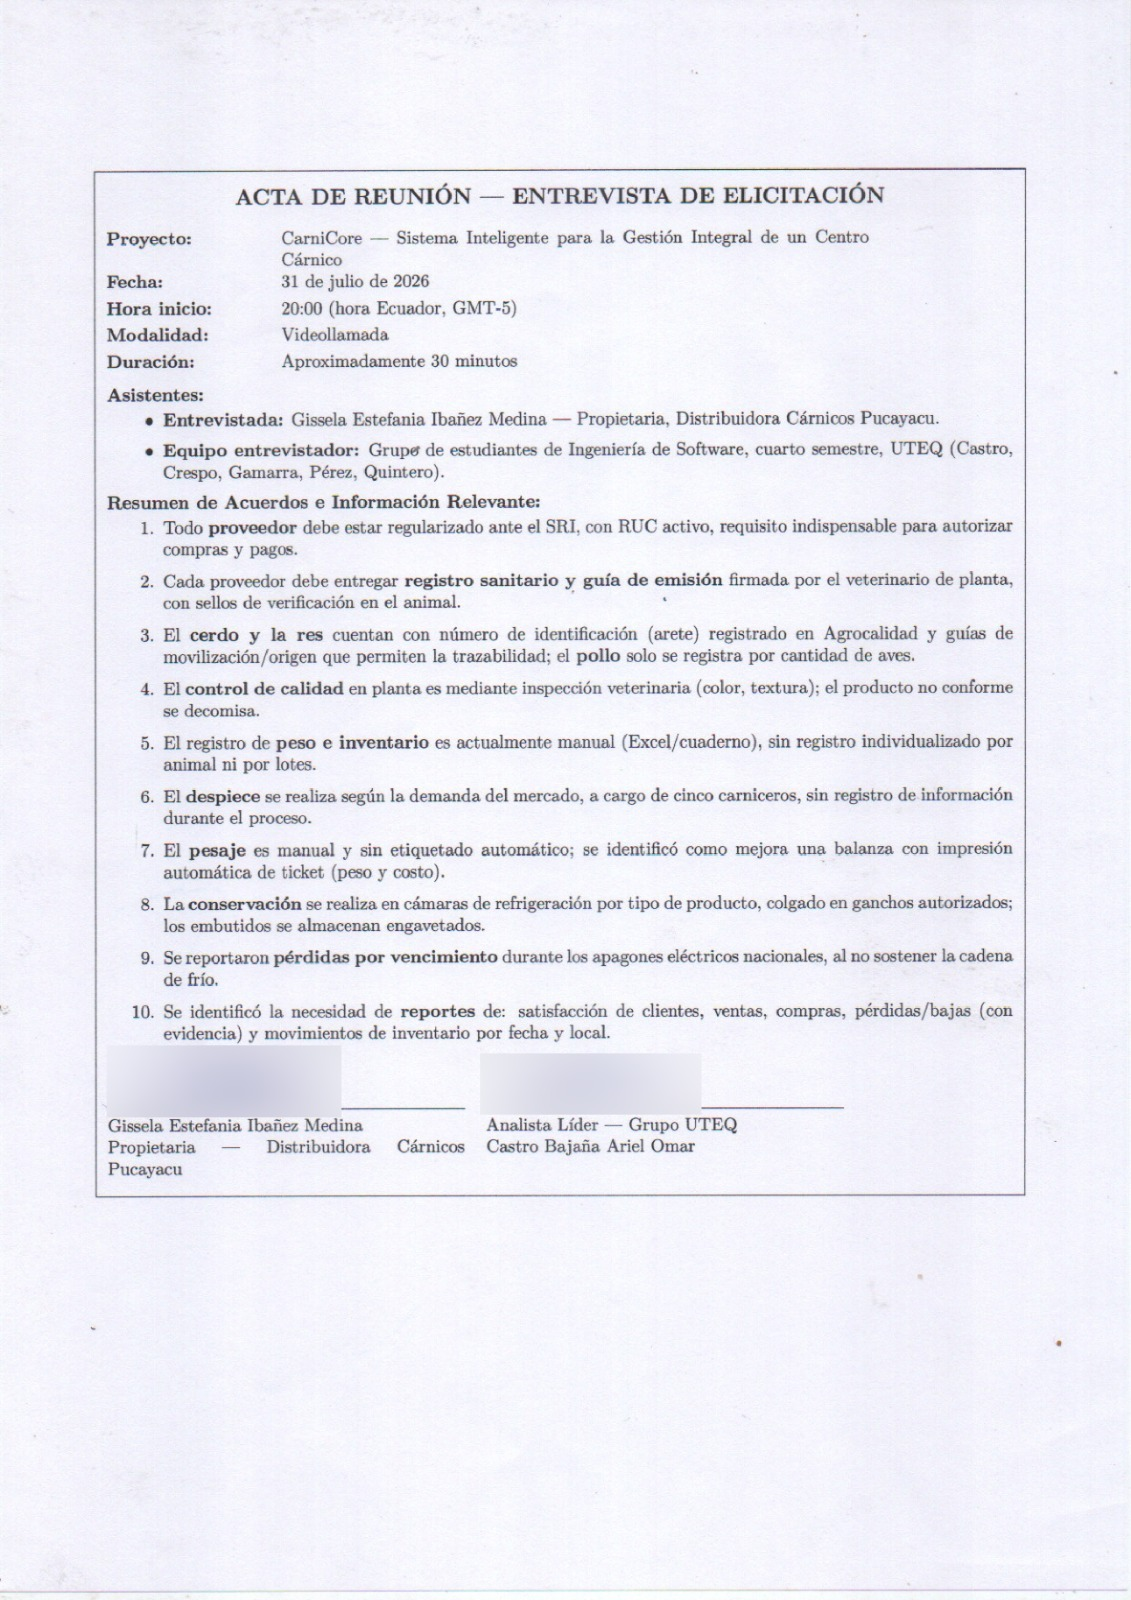
\includegraphics[width=\textwidth,keepaspectratio]{figures/ACTA-05.jpg}
    \label{fig:diagrama_clases}
\end{figure}

%======================================================
\section{Clasificación y priorización de requisitos}
%======================================================
La tabla de clasificación MoSCoW completa de los 25 RF y 15 RNF se presenta de forma unificada en la Sección~5.1 (con Kano y WSJF). Se mantiene la justificación de la Entrega 1B: se priorizan como \textit{Must} los requisitos sin los cuales el sistema no resuelve el problema central (trazabilidad e inventario manual, pérdidas no sustentadas, riesgo regulatorio ante Agrocalidad); como \textit{Should}, los que mejoran significativamente el control gerencial sin bloquear la operación básica; como \textit{Could}, mejoras de valor secundario o diferenciador. No se identifican requisitos \textit{Won't} en esta entrega; las exclusiones de alcance (facturación electrónica SRI, comercio electrónico, IoT de sensores, componentes de IA/AA) permanecen documentadas como fuera de alcance en la Sección~1.2 y en la Sección~3.4.

%======================================================
\section{Repositorio GitHub -- estructura obligatoria}
%======================================================
El repositorio del proyecto debe reflejar exactamente la jerarquía exigida en la Sección~8.1 de la guía de la Entrega 3 (2A): archivos raíz (\texttt{README.md}, \texttt{LICENSE}, \texttt{CITATION.cff}, \texttt{CHANGELOG.md}, \texttt{checksums.sha256}) y las carpetas \texttt{01\_ERS/} (este documento y su \texttt{.tex}/\texttt{referencias.bib}), \texttt{02\_Evidencias/} (con \texttt{00\_Restringido/} cifrado), \texttt{03\_Modelado/}, \texttt{04\_Trazabilidad/}, \texttt{05\_MVP/}, \texttt{06\_Experimento/}, \texttt{07\_Publicacion/} y \texttt{08\_Etica/}.

El repositorio del proyecto está disponible en: \url{https://github.com/EdhuXav/CarniCore_Proyecto_ISR401}


\newpage
\bibliographystyle{plain}
\bibliography{referencias}

\end{document}
